%! TEX program = lualatex
% vim:nospell

%!TEX root = ../main.tex
% vim:nospell

\directlua{pdf.setminorversion(7)}
\RequirePackage{shellesc} % unified shell-escape interface
\RequirePackage[debrief]{silence}
\RequirePackage[l2tabu, orthodox]{nag}

\RequirePackage{xstring}
\StrBetween{\luatexbanner}{\detokenize{n }}{\detokenize{.0 (}}[\luatexversionused] % obtain luatex version used

\providecommand{\pdfxopts}{a-3b,pdf17} % may use options such as a-1a. a-1b
\immediate\write18{rm \jobname.xmpdata} % comment out for non-*nix systems
\begin{filecontents*}{\jobname.xmpdata}
    \Author{Krishnakumar Gopalakrishnan}
\CopyrightURL{https://creativecommons.org/licenses/by-nc-nd/4.0/}
\Copyright{\textcopyright  2018 by Krishnakumar Gopalakrishnan. The copyright  of  this thesis  rests  with the  author  and is  made available  under a  Creative Commons  Attribution Non-Commercial  No Derivatives licence. Researchers are free to copy,  distribute or transmit the thesis on the condition  that they  attribute  it, that  they  do not  use  it for  commercial purposes and that they  do not alter, transform or build upon  it. For any reuse or redistribution,  researchers must make clear  to others the licence  terms of this work.}
\Creator{LuaTeX \luatexversionused\space and pdfx.sty with options \pdfxopts}
\Subject{Lithium ion batteries \sep Mathematical models \sep Electric vehicles \sep Plug-in electric vehicles \sep Electric vehicle industry \sep Electric vehicles--Batteries \sep Battery management systems \sep Battery charging stations (Electric vehicles) \sep Battery industry \sep electrochemistry \sep Electric batteries \sep Numerical calculations \sep Numerical analysis \sep Chemical processes--Mathematical models \sep Simulation methods \sep Computer simulation \sep Computer modeling \sep battery management systems }
\Keywords{lithium-ion batteries \sep electric vehicles \sep mathematical modelling \sep lithium-ion cell \sep electrochemical cell \sep electrolyte model \sep SPM \sep single particle model \sep layer optimisation \sep pouch cell design \sep layer optimisation \sep pseudo-2d model \sep fast charging \sep mathematical models \sep computer simulation }
\pdfxSetCMYKcolorProfileDir{icc_profiles/coated_FOGRA39L_argl.icc}
\pdfxSetRGBcolorProfileDir{icc_profiles/sRGB_IEC61966-2-1_black_scaled.icc}
\Producer{LuaTeX \luatexversionused\space and pdfx.sty with options \pdfxopts}
\PublicationType{PhD Thesis}
\Publisher{Imperial College London}
\Title{Computational modelling of lithium ion batteries for electric vehicle applications: analysis, design and implementation}


\end{filecontents*}

\PassOptionsToPackage{\pdfxopts}{pdfx}
\PassOptionsToPackage{table}{xcolor}
\PassOptionsToPackage{luatex}{pdflscape}
\PassOptionsToPackage{pdfa}{hyperref}

% Options to these packages are passed to them whenever they get loaded
\PassOptionsToPackage{title, titletoc}{appendix}
\PassOptionsToPackage{makeroom}{cancel}
\PassOptionsToPackage{backend=biber, style=numeric-comp, sorting=none, citestyle=numeric-comp, maxbibnames=50, url=true, doi=true, eprint=false, backref=true, backrefstyle=three}{biblatex}
\PassOptionsToPackage{margin=10pt, font=small, labelfont={bf}, labelsep=quad}{caption}
\PassOptionsToPackage{type={CC}, modifier={by-nc-nd}, version={4.0}}{doclicense}
\PassOptionsToPackage{normal}{engord}
\PassOptionsToPackage{inline}{enumitem}
\PassOptionsToPackage{draft}{fixme}
\PassOptionsToPackage{bottom}{footmisc}
\PassOptionsToPackage{luatex, paper=a4paper, hmarginratio=1:1, vmarginratio=1:1, scale=0.75}{geometry}
\PassOptionsToPackage{local, markifdraft}{gitinfo2}
\PassOptionsToPackage{frac, vfrac, multskip}{mathfixs}
\PassOptionsToPackage{section}{placeins}
\PassOptionsToPackage{separate-uncertainty = true, multi-part-units=single, detect-all}{siunitx}
\PassOptionsToPackage{nottoc}{tocbibind}
\PassOptionsToPackage{normalem}{ulem}
\PassOptionsToPackage{no-math, quiet}{fontspec}
\PassOptionsToPackage{warnings-off={mathtools-colon}}{unicode-math}
\PassOptionsToPackage{british}{babel}
\PassOptionsToPackage{final, activate={true, nocompatibility}, factor=1100, stretch=10, shrink=10, babel=true}{microtype}
\PassOptionsToPackage{british}{selnolig}
\PassOptionsToPackage{newfloat=true}{minted}
\PassOptionsToPackage{minted, most}{tcolorbox}
\PassOptionsToPackage{all}{hypcap}
\PassOptionsToPackage{nomain, acronym, xindy}{glossaries-extra}
\PassOptionsToPackage{depth=4, open=true, openlevel=0, numbered=true}{bookmark}
% \PassOptionsToPackage{nameinlink}{cleveref}
\PassOptionsToPackage{hyphenation, lastparline, nosingleletter}{impnattypo}
\PassOptionsToPackage{defaultlines=2, all}{nowidow}

\documentclass[12pt,a4paper,oneside,openright]{book} % using the book document class

%%%%%%%%%% list of packages to be loaded %%%%%%%%%%

% uncommment any commented packages before final submission
\usepackage{afterpage}
\usepackage{algpseudocode}  % http://ctan.org/pkg/algorithmicx
\usepackage{bigints}
\usepackage{cancel}
\usepackage{pdfpages}
\usepackage{tabstackengine} % stackmath macro uses this package

%!TEX root = ../main.tex
% vim:nospell

% useful packages for writing any general  draft document with a small subset of
% packages  only for  book/thesis  style  docs and  another  subset of  packages
% applicable only for luatex
% Most notably, microtype is missing here since it needs to be loaded after babel (which is to be loaded after fontspec)

\usepackage{amsmath}
\usepackage{amsfonts}
\usepackage{amssymb}
\usepackage{anyfontsize} % typically for thesis use; fancy chapter font size and shading
\usepackage{appendix}    % add appendices

\usepackage{babel}       % with british, we get OUP hyphenation material for free
\usepackage{biblatex}    % seems to have strong dependence on csquotes?
\usepackage{booktabs}

\usepackage{caption}     % for improved layout of figure captions with extra margin, smaller font than text
\usepackage{checkend}

% \usepackage[datesep=/,useregional]{datetime2}
\usepackage[datesep=/,style=ddmmyyyy]{datetime2}
% \DTMsetdatestyle{en-GB-numeric}
\usepackage{diffcoeff}   % looks pretty useful for any math-oriented document. Leaving it here

\usepackage{engord}      % an alternative is to use the fmtcount package
\usepackage{enumitem}

\usepackage{fancyhdr}    % Define custom header (before hyperref)
\usepackage{fixme}
\usepackage{flafter}
\usepackage{footmisc}    % typically for thesis use;

\usepackage{geometry}
\usepackage{gitinfo2}
\usepackage{graphicx}    % important to load before fontspec

\usepackage{labelschanged}
\usepackage{lualatex-math}

\usepackage{makecell}
\usepackage{mathtools}
\usepackage{mathfixs}
\usepackage{multicol}
\usepackage{multirow}

\usepackage[section]{placeins} % Defines a \FloatBarrier command

% \usepackage{rotating} % defines a sidewaystable environment
% \usepackage{pdflscape}
\usepackage{lscape}
\usepackage{longtable}
\usepackage{setspace} % Define line spacing

\usepackage{siunitx}
\usepackage{subcaption}

\usepackage{titlesec}  % typically for thesis use;
\usepackage{titletoc}  % typically for thesis use;
\usepackage{threeparttable}
\usepackage{tocbibind} % typically for thesis use; correct page numbers for bib in TOC, nottoc suppresses an entry for TOC itself

\usepackage{ulem}

\usepackage{varwidth}

\usepackage{witharrows}

\usepackage{xfrac}
\usepackage{xpatch} % example use; helpful to replace parens with brackets for backreferencing with biblatex

% ---------- unused packages (but potentially useful) ----------
% \usepackage[backend=biber, style=ieee, sortlocale=en_GB, maxbibnames=50, url=true, doi=true, eprint=true ]{biblatex}
% \usepackage{blindtext}
% \usepackage{chkfloat}
% \usepackage{cite} % incompatible with biblatex
% \usepackage{cmdtrack}
% \usepackage{colortbl} % colortbl cannot be used if xcolor is used
% \usepackage{etoolbox} % not really required if using glossaries package, since this package then gets loaded automatically
% \usepackage{fnpct}
% \usepackage{footnote}
% \usepackage{layouts} % helpful for computing textwidth, textheight etc
% \usepackage{lettrine}
% \usepackage{luabibentry}
% \usepackage{makebox}
% \usepackage[activate={true,nocompatibility},final,tracking=true,factor=1100,stretch=10,shrink=10]{microtype}
% \usepackage{nccmath}
% \usepackage{needspace}
% \usepackage{nolbreaks}
% \usepackage[all,warning]{onlyamsmath} % if using Tikz, please include the calc and babel libraries (known incompatibilities)
% \usepackage{blindtext}
% \usepackage{soulutf8}
% \usepackage{subfiles}
% \usepackage{tablefootnote}
% \usepackage{tabularx}
% \usepackage[table]{xcolor} % loaded by pdfx package (if used) cannot explicitly load colortbl package either before or after
% \usepackage{url}

 % a bit specific to luatex; also includes biblatex

\usepackage{unicode-math} % fontspec after graphicx and babel; https://tex.stackexchange.com/questions/188222/problem-with-babel-and-fontspec; no-math option (math-handling is left to unicode-math); silent to suppress all warnings (even in log file)
%!TEX root = ../main.tex
% vim:nospell

\setmainfont{LibertinusSerif}[%
Extension         = .otf,
Path              = ./fonts/,
UprightFont       = *-Regular,
BoldFont          = *-Bold,
ItalicFont        = *-Italic,
BoldItalicFont    = *-BoldItalic,
Numbers           = {Proportional, Lining},
Ligatures         = {TeX, Common, Required},
SmallCapsFeatures = {Letters = SmallCaps},
% Fractions         = On,
Kerning           = {Uppercase, On},
% FontFace       = {sb}{n}{*-Semibold},
% FontFace       = {sb}{it}{*-SemiboldItalic},
]%

\setsansfont{LibertinusSans}[%
Extension         = .otf,
Path              = ./fonts/,
UprightFont       = *-Regular,
BoldFont          = *-Bold,
ItalicFont        = *-Italic,
BoldItalicFont    = *-BoldItalic,
Numbers           = {Proportional, Lining},
Ligatures         = {TeX, Common, Required},
SmallCapsFeatures = {Letters = SmallCaps},
% Fractions         = On,
Kerning           = {Uppercase, On},
]%

% \setmainfont[Numbers={Proportional},Ligatures={TeX, Common%, Historic, Contextual, Rare, Discretionary
% }]{Libertinus Serif}
% \setsansfont{Libertinus Sans}

\setmonofont{Latin Modern Mono}

% % https://tex.stackexchange.com/questions/103379/minionpro-semibold-medium
% \DeclareRobustCommand\sbseries{\fontseries{sb}\selectfont}
% \DeclareTextFontCommand{\textsb}{\sbseries}

\defaultfontfeatures{ Scale = MatchLowercase }
\defaultfontfeatures[\rmfamily]{ Scale = 1}

% \setmathfont[bold-style = ISO]{LibertinusMath-Regular.otf} % https://github.com/libertinus-fonts/libertinus/issues/20
\setmathfont{LibertinusMath-Regular.otf}[%
Path       = ./fonts/,
bold-style = ISO, % https://github.com/libertinus-fonts/libertinus/issues/20
]%

\setmathfont{libertinusmath-bold.otf}[%
Path       = ./fonts/,
bold-style = ISO, % https://github.com/libertinus-fonts/libertinus/issues/20
version    = bold,
]%

% \setmathfont[math-style=upright,range={`e,`i}]{Latin Modern Math}
% \setmathfont[range={\mathunder,\triangleq},Scale=MatchUppercase]{STIX2Math.otf}
\setmathfont[range = {\mathunder,\triangleq,\underbrace},Scale = MatchUppercase]{Latin Modern Math}

 % selection of unicode text and math fonts

\usepackage{ragged2e}  % should be loaded after the body font and size have been established
\usepackage{microtype} % if using option babel=true, babel must be loaded before microtype; microtype must be loaded after font selection (after fontspec)

\usepackage{selnolig}  % luatex package;  should go after loading babel

\usepackage{float} % Loading order is important here https://tex.stackexchange.com/questions/435529/correct-loading-order-of-package-newfloat-along-with-hyperref-and-algorithmic-pa/435597#435597
\usepackage{minted}
\usepackage{tcolorbox}
\usepackage{csquotes}    % The fvextra package is loaded by minted, so you should load minted before csquotes; has a strong dependency with biblatex
\usepackage{chemformula} % uses tikz arrows

%!TEX root = ../main.tex
% vim: nospell

\usepackage{pdfx}
% https://tex.stackexchange.com/questions/449470/pdfx-package-incompatibility-with-bookmark-package-when-using-luatex-engine/449508#449508
\ifluatex
    \pdftrue
\fi

\usepackage{hyperxmp} % comment out if using the pdfx package
% \usepackage{hyperref} % comment out if using the pdfx package

\hypersetup{%
    anchorcolor        = black,
    baseurl            = {http://spiral.imperial.ac.uk/},
    breaklinks         = true,
    citecolor          = [RGB]{0,68,136}, % https://personal.sron.nl/https://personal.sron.nl/pault/#fig:scheme_highcontrastpault/#fig:scheme_highcontrast
    colorlinks         = true,
    final              = true,
    linkcolor          = [RGB]{0,68,136}, % https://personal.sron.nl/https://personal.sron.nl/pault/#fig:scheme_highcontrastpault/#fig:scheme_highcontrast
    linktocpage        = true,
    pdfauthor          = {Krishnakumar Gopalakrishnan},
    pdfauthortitle     = {PhD student},
    pdfapart           = {3},
    pdfborderstyle     = {/S/U/W 1},
    pdfcaptionwriter   = {Krishnakumar Gopalakrishnan},
    pdfcenterwindow    = true,
    pdfcontactaddress  = {Mechanical Engineering Dept, Exhibition Road, City and Guild Building, Imperial College London, South Kensington},
    pdfcontactcity     = {London, United Kingdom},
    pdfcontactcountry  = {United Kingdom},
    pdfcontactemail    = {krishnak at vt dot edu},
    pdfcontactpostcode = {SW7 2AZ},
    pdfcontactregion   = {Greater London},
    pdfcontacturl      = {https://krishnakumarg.gitlab.io, https://www.linkedin.com/in/krishnakumargopalakrishnan},
    pdfcopyright       = {\textcopyright{} 2019 by Krishnakumar Gopalakrishnan. The    copyright    of    this     thesis    rests    with    the    author. Unless   otherwise    indicated,   its    contents   are    licensed   under a   Creative Commons   Attribution-NonCommercial-NoDerivatives  4.0   International  (CC BY-NC-ND 4.0) Licence. Under this licence, you may  copy and redistribute the material in any medium or format on the condition that: you credit the author, do not use it for commercial purposes  and do not distribute  modified versions of the  work. When reusing or sharing this work, ensure you  make the licence terms clear to others by naming  the licence and linking  to the licence text.  Please seek permission from the copyright  holder for uses of  this work that are not  included in this licence or permitted under UK Copyright Law.},
    pdfcreator         = {LaTeX with hyperref},
    pdfdisplaydoctitle = true,
    pdffitwindow       = true,
    pdfkeywords        = {lithium-ion batteries, electric vehicles, mathematical modelling, lithium-ion cell, electrochemical cell, electrolyte model, SPM, single particle model, layer optimisation, pouch cell design, layer optimisation, pseudo-2d model, fast charging, mathematical models, computer simulation},
    pdflang            = {en-GB-oxendict},
    pdflicenseurl      = {https://creativecommons.org/licenses/by-nc-nd/4.0/},
    pdfmetalang        = {en-GB-oxendict},
    pdfproducer        = {LuaTeX-\luatexversionused},
    pdfsource          = {},
    pdfstartview       = {Fit},
    pdfsubject         = {Lithium ion batteries, Mathematical models, Electric vehicles, Plug-in electric vehicles, Electric vehicle industry, Electric vehicles--Batteries, Battery management systems, Battery charging stations (Electric vehicles), Battery industry, electrochemistry, Electric batteries, Numerical calculations, Numerical analysis, Chemical processes--Mathematical models, Simulation methods, Computer simulation, Computer modeling, battery management systems},
    pdftitle           = {Computational modelling of lithium ion batteries for electric vehicle applications: analysis, design and implementation},
    pdftoolbar         = true,
    plainpages         = false,
    pdfencoding        = auto,
    unicode            = true,
    urlcolor           = [RGB]{0,68,136}, % https://personal.sron.nl/https://personal.sron.nl/pault/#fig:scheme_highcontrastpault/#fig:scheme_highcontrast
}%


% ---------- packages to be loaded after hyperref ----------%

\usepackage{nameref}
\usepackage{algorithm} % http://ctan.org/pkg/algorithms
\usepackage{hypcap} % to be loaded after hyperref. fix hyperref links to jump directly to Table or Figure

\usepackage{pdftexcmds} % not required if using pdfx package

\usepackage{glossaries-extra} % should be loaded after hyperref, but before cleveref % consider 'symbols' option

\usepackage{hypdestopt} % seems to have problems with pdfx package?

\usepackage{bookmark} % improves bookmarks handling. % More features and faster updated bookmarks.
\usepackage{cleveref}

% \usepackage{showframe}
% \usepackage[noframe]{showframe}
\newcommand{\blackurl}{\hypersetup{urlcolor=black}}%
\newcommand{\regularurl}{\hypersetup{urlcolor=[RGB]{0,68,136}}}%

  % hyperref, nameref, algoriothm, hypcap, bookmark, glossaries, cleveref, showframe
\usepackage{doclicense}

\usepackage{impnattypo}
\usepackage{nowidow}

%---------- end of package loading ----------%


%---------- begin custom commands ----------%
%!TEX root = ../main.tex
% vim:nospell ft=tex

\definecolor{mintedbg}{rgb}{0.95,0.95,0.95}
\definecolor{imperialraspberry}{RGB}{145,0,72}

\definecolor{imperialbrick}{RGB}{165,25,0}
\definecolor{sepiadvipsnames}{RGB}{99,29,11}
\definecolor{imperialnavy}{RGB}{0,33,71}
% \definecolor{brickreddvipsnames}{RGB}{173,51,38}
% \definecolor{mahoganydvipsnames}{RGB}{161,53,40}

\definecolor{imperialblue}{RGB}{0,62,116}
\definecolor{cbrewerdarkblue}{RGB}{49,130,189}
\definecolor{viridistendarkblue}{RGB}{56,88,140}
\definecolor{viridistwentyblueseven}{RGB}{49,103,142}
\definecolor{viridistwentybluesix}{RGB}{54,91,141}
\definecolor{viridistwentybluefive}{RGB}{60,78,138}
\definecolor{viridistenlighterblue}{RGB}{45,111,142}
\definecolor{imperiallightblue}{RGB}{0,110,175}
\definecolor{imperialnewblue}{RGB}{0,86,146}

\definecolor{imperialdarkgreen}{RGB}{2,137,59}
\definecolor{imperialprocessblue}{RGB}{0,133,202}

\definecolor{imperiallightgray}{RGB}{235,238,238}
\definecolor{cbrewerlightgray}{RGB}{240,240,240}
\definecolor{cbrewerintergray}{RGB}{189,189,189}
\definecolor{imperialcoolgray}{RGB}{157,157,157}

\definecolor{intermediategray}{RGB}{196,196,196}
\definecolor{cbrewerdarkgray}{RGB}{99,99,99}
\definecolor{lightintergray}{RGB}{215,217,217}

%!TEX root = ../main.tex
% vim:nospell ft=tex

\newcommand{\effdelta}{\ensuremath{{\text{eff}_\delta}}}
\newcommand{\effj}{\ensuremath{{\text{eff}_j}}}
\newcommand{\efflambda}{\ensuremath{{\text{eff}_\lambda}}}
\newcommand{\effmu}{\ensuremath{{\text{eff}_\mu}}}
\newcommand{\effn}{\ensuremath{{\text{eff}_n}}}
\newcommand{\effp}{\ensuremath{{\text{eff}_p}}}
\newcommand{\effs}{\ensuremath{{\text{eff}_s}}}
\newcommand{\elambda}{\ensuremath{{\text{e}_\lambda}}}
\newcommand{\eneg}{\ensuremath{\text{e,neg}}}
\newcommand{\ensub}{\ensuremath{\text{e,n}}}
\newcommand{\epos}{\ensuremath{\text{e,pos}}}
\newcommand{\epsub}{\ensuremath{\text{e,p}}}
\newcommand{\essub}{\ensuremath{\text{e,s}}}

\newcommand{\jinnegposordered}{\ensuremath{j  \in  \left(\text{neg, pos}\right)}}
\newcommand{\jinnegpos}{\ensuremath{j  ∈  \left\{\text{neg, pos}\right\}}}
\newcommand{\jinnegseppos}{\ensuremath{j  ∈  \left\{\text{neg, sep, pos}\right\}}}
\newcommand{\jinnsp}{\ensuremath{j  ∈  \left\{\text{n,s,p}\right\}}}
\newcommand{\jinpossepneg}{\ensuremath{j  ∈  \left\{\text{pos, sep, neg}\right\}}}
\newcommand{\jr}{\ensuremath{{\text{r}_j}}}
\newcommand{\lambdainnegpos}{\ensuremath{\lambda  ∈  \left\{\text{neg, pos}\right\}}}
\newcommand{\lambdainnegseppos}{\ensuremath{\lambda  \in  \{\text{neg, sep, pos}\}}}
\newcommand{\lambdar}{\ensuremath{{\text{r}_\lambda}}}
\newcommand{\maxj}{\ensuremath{{100\%_j}}}
\newcommand{\maxneg}{\ensuremath{{100\%_\text{neg}}}}
\newcommand{\maxpos}{\ensuremath{{100\%_\text{pos}}}}
\newcommand{\minj}{\ensuremath{{0\%_j}}}
\newcommand{\minneg}{\ensuremath{{0\%_\text{neg}}}}
\newcommand{\minpos}{\ensuremath{{0\%_\text{pos}}}}
\newcommand{\muinnegseppos}{\ensuremath{\mu  \in  \{\text{neg, sep, pos}\}}}
\newcommand{\negr}{\ensuremath{{\text{r}_\text{neg}}}}
\newcommand{\nj}{\ensuremath{{\text{n}_j}}}
\newcommand{\nneg}{\ensuremath{{\text{n}_\text{neg}}}}
\newcommand{\npos}{\ensuremath{{\text{n}_\text{pos}}}}
\newcommand{\pj}{\ensuremath{{\text{p}_j}}}
\newcommand{\plambda}{\ensuremath{{\text{p}_\lambda}}}
\newcommand{\pneg}{\ensuremath{{\text{p}_\text{neg}}}}
\newcommand{\posr}{\ensuremath{{\text{r}_\text{pos}}}}
\newcommand{\ppos}{\ensuremath{{\text{p}_\text{pos}}}}
\newcommand{\refflambda}{\ensuremath{{\text{r,eff}_\lambda}}}
\newcommand{\sefflambda}{\ensuremath{{\text{s,eff}_\lambda}}}
\newcommand{\sjavg}{\ensuremath{{\text{s,avg}_j}}}
\newcommand{\sjmax}{\ensuremath{{\text{s,max}_j}}}
\newcommand{\sjsurf}{\ensuremath{{\text{s,surf}_j}}}
\newcommand{\sj}{\ensuremath{{\text{s}_j}}}
\newcommand{\slambdamax}{\ensuremath{{\text{s,max}_\lambda}}}
\newcommand{\slambdasurf}{\ensuremath{{\text{s,surf}_\lambda}}}
\newcommand{\slambda}{\ensuremath{{\text{s}_\lambda}}}
\newcommand{\snegmax}{\ensuremath{{\text{s,max}_\text{neg}}}}
\newcommand{\snegmin}{\ensuremath{{\text{s,min}_\text{neg}}}}
\newcommand{\snegsurf}{\ensuremath{{\text{s,surf}_\text{neg}}}}
\newcommand{\sneg}{\ensuremath{\text{s,neg}}}
\newcommand{\snsub}{\ensuremath{\text{s,n}}}
\newcommand{\sposmax}{\ensuremath{{\text{s,max}_\text{pos}}}}
\newcommand{\spossurf}{\ensuremath{{\text{s,surf}_\text{pos}}}}
\newcommand{\spos}{\ensuremath{\text{s,pos}}}
\newcommand{\spsub}{\ensuremath{\text{s,p}}}
\newcommand{\tplus}{\ensuremath{{t^0_\text{+}}}}

%!TEX root = ../main.tex
% vim:nospell ft=tex

% For unbroken lines in algorithmicx/algpseudocode when typesetting display math

% other alternative: https://tex.stackexchange.com/questions/110431/problems-with-vertical-lines-in-algorithmicx?noredirect=1&lq=1
% https://tex.stackexchange.com/questions/301462/why-are-vertical-rules-dashed-sometimes-with-algorithmic-package
%%%%%%%%%% https://tex.stackexchange.com/questions/350399/indentation-scope-lines-broken-in-algpseudocode%%%%%%%%%
\newcommand*{\algrule}[1][\algorithmicindent]{\hspace*{.2em}{\color{cbrewerdarkgray}\vrule\vrule
width 0pt height \baselineskip depth .1618\baselineskip\hspace*{\dimexpr#1-.5em}}}

\makeatletter
\newcount\ALG@printindent@tempcnta
\def\ALG@printindent{%
    \ifnum \theALG@nested>0% is there anything to print
        \ifx\ALG@text\ALG@x@notext% is this an end group without any text?
            % do nothing
    \else
        \unskip
        % draw a rule for each indent level
        \ALG@printindent@tempcnta=1
        \loop
        \algrule[\csname ALG@ind@\the\ALG@printindent@tempcnta\endcsname]%
        \advance \ALG@printindent@tempcnta 1
        \ifnum \ALG@printindent@tempcnta<\numexpr\theALG@nested+1\relax% can't do <=, so add one to RHS and use < instead
            \repeat
        \fi
    \fi
}%
% needs etoolbox, but this should have been already loaded with glossaries
\patchcmd{\ALG@doentity}{\noindent\hskip\ALG@tlm}{\ALG@printindent}{}{\errmessage{failed to patch}}
\makeatother

\AtBeginEnvironment{algorithmic}{\lineskip0pt}
%%%%%%%%%% https://tex.stackexchange.com/questions/350399/indentation-scope-lines-broken-in-algpseudocode%%%%%%%%%


\algnewcommand\algorithmicinput{\textbf{Initialise:}}
\algnewcommand\Initialise{\item[\algorithmicinput]}

\algnewcommand\algorithmicdata{\textbf{User data:}}
\algnewcommand\Userdata{\item[\algorithmicdata]}

\algnewcommand\algorithmicfulllinecomment{\qquad\quad  \scriptsize \textit{Note:}}
\algnewcommand\FullComment{\item[\algorithmicfulllinecomment]}

\makeatletter
\algrenewcommand\ALG@beginalgorithmic{\footnotesize}
\algrenewcommand\algorithmiccomment[2][\footnotesize]{{#1\hfill\(\triangleright\) #2}}
\makeatother

\algblockdefx[NAME]{ISR}{END}%
[2][Unknown]{\textbf{begin} \textproc{Interrupt Service Routine} #1(#2)}%
{\textbf{return} \Comment[\footnotesize]{resume suspended line in \textsc{Main()}}}

\algblockdefx[NAME]{OutputEqn}{EndOutputEqn}%
[2][\textbf{x}]{\textbf{subroutine} \textproc{ComputeCellVoltage}(#2)}%
{\textbf{return} $V_\text{cell}$ \Comment[\footnotesize]{resume suspended line in \textproc{Simulate\gls{spm}}}}

\newsavebox{\algboxA}
\newsavebox{\algboxB}

\makeatletter
\@addtoreset{algorithm}{chapter}% algorithm counter resets every chapter
\makeatother
\renewcommand{\thealgorithm}{\thechapter.\arabic{algorithm}}% Algorithm # is <chapter>.<algorithm>

\providecommand\algorithmname{algorithm}
\captionsetup[ruled]{font=small,labelfont={bf},labelsep=quad}

\newcommand{\tempcaption}{}% stores the caption
\newcommand{\templabel}{}% stores the label

\newenvironment{customalgo}[3][0.7\textwidth]
{%
    \begin{minipage}{#1}
        \begin{algorithm}[H]
            \centering
            \gdef\tempcaption{#2}% store the caption so we can use it later
            \gdef\templabel{#3}% store the label so we can use it later
            \begin{algorithmic}[1]
            }%
            {%
            \end{algorithmic}
            \caption{\tempcaption}% use the stored caption
            \label{\templabel}
        \end{algorithm}
    \end{minipage}
    % \smallskip
}%

% extent of line-spacing in algorithms
\let\Algorithm\algorithm
\renewcommand\algorithm[1][]{\Algorithm[#1]\setstretch{1.2390625}}

% % https://tex.stackexchange.com/questions/64674/coloring-lines-in-an-algorithm
% \makeatletter
% \newcommand{\algcolor}[2]{%
%     \hskip-\ALG@thistlm\colorbox{#1}{\parbox{\dimexpr\linewidth-2\fboxsep}{\hskip\ALG@thistlm\relax #2}}%
% }
% \newcommand{\algemph}[1]{\algcolor{cbrewerintergray}{#1}}
% \makeatother


%  https://tex.stackexchange.com/questions/64674/coloring-lines-in-an-algorithm
\makeatletter
% code borrowed from Andrew Stacey; See
% https://tex.stackexchange.com/a/50054/3954
\tikzset{%
    remember picture with id/.style={%
        remember picture,
        overlay,
        save picture id=#1,
    },
    save picture id/.code={%
        \edef\pgf@temp{#1}%
        \immediate\write\pgfutil@auxout{%
        \noexpand\savepointas{\pgf@temp}{\pgfpictureid}}%
    },
    if picture id/.code args={#1#2#3}{%
        \@ifundefined{save@pt@#1}{%
            \pgfkeysalso{#3}%
            }{
            \pgfkeysalso{#2}%
        }
    }
}

\def\savepointas#1#2{%
    \expandafter\gdef\csname save@pt@#1\endcsname{#2}%
}

\def\tmk@labeldef#1,#2\@nil{%
    \def\tmk@label{#1}%
    \def\tmk@def{#2}%
}

\tikzdeclarecoordinatesystem{pic}{%
    \pgfutil@in@,{#1}%
    \ifpgfutil@in@%
        \tmk@labeldef#1\@nil
    \else
        \tmk@labeldef#1,(0pt,0pt)\@nil
    \fi
    \@ifundefined{save@pt@\tmk@label}{%
        \tikz@scan@one@point\pgfutil@firstofone\tmk@def
        }{%
        \pgfsys@getposition{\csname save@pt@\tmk@label\endcsname}\save@orig@pic%
        \pgfsys@getposition{\pgfpictureid}\save@this@pic%
        \pgf@process{\pgfpointorigin\save@this@pic}%
        \pgf@xa=\pgf@x
        \pgf@ya=\pgf@y
        \pgf@process{\pgfpointorigin\save@orig@pic}%
        \advance\pgf@x by -\pgf@xa
        \advance\pgf@y by -\pgf@ya
    }%
}

\makeatother
% end of Andrew's code

% main command to draw the colored background
\newcounter{mymark}
\newcommand\ColorLine{%
    \stepcounter{mymark}%
    \tikz[remember picture with id=mark-\themymark,overlay] {;}%
    \begin{tikzpicture}[remember picture,overlay]%
        \filldraw[cbrewerintergray]%
            let \p1=(pic cs:mark-\themymark),
            \p2=(current page.east)  in
            ([xshift=-0.1em,yshift=-1.0ex]0,\y1)  rectangle ++([xshift=-2.525cm]\x2,\baselineskip);
    \end{tikzpicture}%
}%



 % for typesetting of algorithms
%!TEX root = ../main.tex
% vim:nospell

% \addbibresource{backmatter/thesis_refs.bib}
\ShellEscape{biber --tool backmatter/thesis_refs.bib} % deduplicate bibtex entries
\addbibresource{backmatter/thesis_refs_bibertool.bib}
\addbibresource{backmatter/thesis_refs_joint.bib}

% https://brianbuccola.com/how-to-cite-in-latex-without-the-citation-appearing-in-the-bibliography/
\DeclareBibliographyCategory{ignore}
\addtocategory{ignore}{Gopalakrishnan2018joint}

\renewcommand*{\bibfont}{\small} % make Bibliography left aligned, not justified

\DeclareSourcemap{
    \maps[datatype=bibtex]{
        \map{
            \step[fieldsource=doi,final]
            \step[fieldset=url,null]
        }
    }
}

\DefineBibliographyStrings{english}{%
    backrefpage = {cited on page},% originally "cited on page"
    backrefpages = {cited on pages},% originally "cited on pages"
}

\xpatchbibmacro{pageref}{parens}{brackets}{}{}   % helpful to replace parens with brackets for backreferencing with biblatex % needs xpatch

% \renewbibmacro*{pageref}{\iflistundef{pageref}{}{\printtext[brackets]{\printlist[​pageref][-\value{listtotal}]{pageref}}}}

\DeclareSourcemap{
    \maps[datatype=bibtex]{
        \map[overwrite]{
            \step[fieldsource=month, match=\regexp{\Ajan\Z}, replace=1]
            \step[fieldsource=month, match=\regexp{\Afeb\Z}, replace=2]
            \step[fieldsource=month, match=\regexp{\Amar\Z}, replace=3]
            \step[fieldsource=month, match=\regexp{\Aapr\Z}, replace=4]
            \step[fieldsource=month, match=\regexp{\Amay\Z}, replace=5]
            \step[fieldsource=month, match=\regexp{\Ajun\Z}, replace=6]
            \step[fieldsource=month, match=\regexp{\Ajul\Z}, replace=7]
            \step[fieldsource=month, match=\regexp{\Aaug\Z}, replace=8]
            \step[fieldsource=month, match=\regexp{\Asep\Z}, replace=9]
            \step[fieldsource=month, match=\regexp{\Aoct\Z}, replace=10]
            \step[fieldsource=month, match=\regexp{\Anov\Z}, replace=11]
            \step[fieldsource=month, match=\regexp{\Adec\Z}, replace=12]
        }
    }
}


% https://tex.stackexchange.com/questions/113039/trying-to-suppress-urls-with-biblatex-using-a-simple-persons-method
% \AtEveryCitekey{\clearfield{url}}

% https://tex.stackexchange.com/questions/46787/is-there-a-way-to-prevent-urls-from-appearing-in-biblatex-citations
\AtEveryCitekey{%
    \clearfield{url}%
    \clearfield{urlyear}%
    \clearfield{doi}%
}%
\renewbibmacro*{in:}{}


% https://tex.stackexchange.com/questions/24979/citing-authors-full-name-in-biblatex
\DeclareCiteCommand*{\citeauthor}
{\defcounter{maxnames}{99}%
    \defcounter{minnames}{99}%
    \defcounter{uniquename}{2}%
    \boolfalse{citetracker}%
    \boolfalse{pagetracker}%
\usebibmacro{prenote}}
{\ifciteindex{\indexnames{labelname}}{}%
    \printnames{labelname}}
    {\multicitedelim}
    {\usebibmacro{postnote}}


% \renewcommand*{\mkbibnamefirst}[1]{\edef\firstname{#1}\expandafter\first{\firstname}}
\renewcommand*{\mkbibnamegiven}[1]{\edef\firstname{#1}\expandafter\first{\firstname}}

\def\bibnamedelima{ }%
\def\bibnamedelimb{ }%

\makeatletter
\def\@empty{}
\def\first#1{\expandafter\@first#1 \@nil}
\def\@first#1 #2\@nil{#1\addspace%
  \if\relax\detokenize{#2}\relax\else\@initials#2\@nil\fi}
\def\initials#1{\expandafter\@initials#1 \@nil}
\def\@initials#1 #2\@nil{%
  \initial{#1}%
  \def\NextName{#2}%
  \ifx\@empty\NextName\relax%
  \else\bibinitdelim \@initials#2\@nil\fi}
\def\initial#1{\expandafter\@initial#1\@nil}
\def\@initial#1#2\@nil{#1\bibinitperiod}
\makeatother


% \makeatletter
% \DeclareCiteCommand{\longfullcite}
% {\usebibmacro{prenote}}
% {\usedriver
%     {\c@maxnames\blx@maxbibnames\relax
%     \DeclareNameAlias{sortname}{default}}
% {\thefield{entrytype}}}
% {\multicitedelim}
% {\usebibmacro{postnote}}
% \makeatother

% \newcommand{\longfullcite}{%
%     \AtNextCite{\defcounter{maxnames}{99}}%
% \fullcite}

\newcommand{\printpublication}[1]{\AtNextCite{\defcounter{maxnames}{99}}\fullcite{#1}}

\DeclareBibliographyAlias{software}{online}

% https://tex.stackexchange.com/questions/468623/indicating-joint-first-authorship-through-special-markup-in-biblatex-biber/468634#468634
\renewcommand*{\mkbibnamefamily}[1]{%
    \ifitemannotation{jointfirst}
        {\uline{\textbf{#1}}}
    {#1}}

\renewcommand*{\mkbibnamegiven}[1]{%
    \ifitemannotation{jointfirst}
        {\uline{\textbf{#1}}}
    {#1}}
     % 'bib' file goes in here
%!TEX root = ../main.tex
% vim:nospell ft=tex

\DeclareGraphicsExtensions{.pdf, .png, .jpg, .jpeg} % GIF doesn't work??

%!TEX root = ../main.tex
% vim:nospell ft=tex

\renewcommand{\CancelColor}{\color{imperialbrick}}
     % uses a predefined color

%!TEX root = ../main.tex
% vim:nospell ft=tex

\DeclareCaptionLabelSeparator{note}{\footnotemark \hspace*{0.5em}}

%!TEX root = ../main.tex
% vim:nospell ft=tex

\crefname{listing}{\MakeLowercase{\listingname}}{\MakeLowercase{\listingname s}}
\crefname{appchap}{appendix}{appendices}
\crefname{filePrg}{listing}{listings}
\Crefname{filePrg}{Listing}{Listings}

\newcommand{\crefrangeconjunction}{--}
\crefrangeformat{equation}{eqs.~(#3#1#4)--(#5#2#6)}


%!TEX root = ../main.tex
% vim:nospell ft=tex

\makeatletter
\newcommand{\monthyeardate}{%
  \DTMenglishmonthname{\@dtm@month} \@dtm@day, \@dtm@year
}
\makeatother

%!TEX root = ../main.tex
% vim:nospell ft=tex

% \diffset[p-delims = . |, p-nudge = 0]

\diffdef { p }
{
    op-symbol = \partial ,
    left-delim = \left .,
    right-delim = \right | ,
    subscr-nudge = 0 mu
}

%!TEX root = ../main.tex
% vim:nospell ft=tex

\setlist[enumerate,itemize,description]{topsep=0em}

\newcounter{descriptcount}
\newlist{enumdescriptnum}{description}{1}
\setlist[enumdescriptnum] {%
    before={\setcounter{descriptcount}{0}%
    \renewcommand*\thedescriptcount{\alph{descriptcount}.}}
    ,font=\footnotesize{\bfseries\stepcounter{descriptcount}\thedescriptcount~}
}


\newcommand{\customenum}[2]{
\item[$ \symbf{#1}\  (\times #2)$]
}


%!TEX root = ../main.tex
% vim:nospell ft=tex

\newcommand{\setFancyHdr}{
    \pagestyle{fancy}
    \renewcommand{\chaptermark}[1]{\markboth{\MakeUppercase{\thechapter. ##1 }}{}}
    \renewcommand{\sectionmark}[1]{\markright{\thesection\ ##1}}
    \fancyhf{}
    \fancyhead[R]{\bfseries\rightmark}
    \fancyfoot[C]{\thepage}
    \fancypagestyle{plain}{
        \fancyhead{}
        \renewcommand{\headrulewidth}{0pt}
    }
}

\setlength{\headheight}{14.5pt}
\setFancyHdr

\renewcommand{\headrulewidth}{\iffloatpage{0pt}{0.4pt}}


%!TEX root = ../main.tex
% vim:nospell ft=tex

\fxsetup{theme=color, marginface=\singlespacing \scriptsize}

\definecolor{fxnote}{RGB}{165,25,0} % imperialbrick (duplicating the color-line here, since `fxnote' is the specific color-name hard-coded by the fxnote package)

%!TEX root = ../main.tex
% vim:nospell ft=tex

% https://tex.stackexchange.com/questions/32819/draw-box-with-colored-background-and-linebreaks-which-adjusts-to-the-text-width
\newcommand\MyCBox[1]{%
      \colorbox{cbrewerfourclssor}{\begin{varwidth}{\dimexpr\linewidth-2\fboxsep}#1\end{varwidth}}}

\renewcommand{\gitMarkFormat}{\color{imperialraspberry} \small}
\renewcommand{\gitMark}{Author: {Krishnakumar Gopalakrishnan}, Imperial College London\, \textbullet{}\, \MyCBox{Confidential (Under Embargo)} \\ Typeset by \StrBehind{\luatexbanner}{\detokenize{This is}}{}  engine using the \LaTeX{} macro format}
\renewcommand{\gitMarkPref}{PhD Thesis}


%!TEX root = ../main.tex
% vim:nospell ft=tex

% \renewcommand*{\glstextformat}[1]{\textsf{#1}}
\renewcommand*{\glstextformat}[1]{\textcolor{black}{#1}} % link coloring to match normal text, ie black
\preto\chapter{\glsresetall} % expand acronyms every chapter https://tex.stackexchange.com/questions/435617/glossaries-expand-acronyms-for-first-time-use-within-each-chapter/435680#435680

% \glsdisablehyper
% \newglossary[slg]{symbolslist}{syi}{syg}{Symbols}

% \newglossarystyle{custom_acronyms}
% {
%     \setglossarystyle{long3colheader}%
%     \renewcommand*{\glossaryheader}{}%
%     \renewcommand{\glossentry}[2]{%
%         \textbf{\glsentryitem{##1}\glstarget{##1}{\glossentryname{##1}}}
%         & \glossentrydesc{##1}
%         & {\hspace*{\fill} ##2}
%     \tabularnewline}%
% }

% \renewcommand{\glossarypreamble}{\footnotesize}
% \renewcommand{\glossarypreamble}{\small}
\setglossarypreamble[acronym]{\small}
\setglossarypreamble[symbols]{\normalsize}
% \renewcommand\glstreepredesc{\qquad}

% https://tex.stackexchange.com/questions/118182/selectively-turn-off-hyperref-links-for-citations
\newcommand*{\nolink}[1]{%
      {\protect\NoHyper#1\protect\endNoHyper}%
  }

\glssetcategoryattribute{acronym}{nohyperfirst}{true} % no hyperlink on first use for entries with category=acronym % https://tex.stackexchange.com/questions/434160/line-break-long-glossaries-entry-when-using-hyperref-and-latex-dvips-ps2pdf
\setabbreviationstyle[acronym]{long-short} % applicable only for glossaries-extra.sty

\GlsXtrLoadResources[
src={frontmatter/acronyms},%
selection={all},
type=acronym,% put these entries in the 'acronym' glossary
save-locations=false% don't save locations
]

% assign titles to group labels:
\glsxtrsetgrouptitle{latin}{List of Latin Symbols}
\glsxtrsetgrouptitle{greek}{List of Greek Symbols}
\glsxtrsetgrouptitle{generic}{Other Generic Nomenclature}

\GlsXtrLoadResources[
src={frontmatter/latin-symbols},
sort={letter-lowerupper},
type=symbols,
selection={all},
category={same as entry},% set the category to the entry type
group={latin},% assign group label
set-widest,% needed for 'alttree' styles
save-locations=false
]

\GlsXtrLoadResources[
src={frontmatter/greek-symbols},% entries in 'greek-symbols.bib'
type=symbols,% put these entries in the 'symbols' glossary
selection={all},
category={same as entry},% set the category to the entry type
group={greek},% assign group label
set-widest,% needed for 'alttree' styles
save-locations=false% don't save locations
]

\GlsXtrLoadResources[
src={frontmatter/generic-symbols},
sort={en-GB},
type=symbols,
selection={all},
category={same as entry},% set the category to the entry type
group={generic},% assign group label
set-widest,% needed for 'alttree' styles
save-locations=false
]

\renewcommand{\glsnamefont}[1]{\textbf{#1}} % to bold-face acronym header with style=super
\glssetcategoryattribute{symbol}{glossdescfont}{normalsize} % https://tex.stackexchange.com/questions/303888/different-formatting-for-acronyms-and-glossary-entries


%!TEX root = ../main.tex
% vim:nospell ft=tex

% https://tex.stackexchange.com/questions/304449/combine-minted-and-tcolorbox-for-code-from-file-inputminted/304691#304691
% https://tex.stackexchange.com/questions/304449/combine-minted-and-tcolorbox-for-code-from-file-inputminted/304975#304975
\newcounter{filePrg}

\newtcbinputlisting[use counter=filePrg,number within=chapter,list inside=mypyg]{\matlabcodelisting}[3][]{%
    listing engine=minted,
    minted language=matlab,
    % minted style=algol_nu, % xcode,emacs, perldoc, pastie, borland, vs, vim, tango
    listing file={#2},
    title=\small{\textbf{Listing \thetcbcounter}\quad {#1}},
    % fonttitle=\bfseries,
    listing only,
    list entry={\protect\numberline{\thetcbcounter} #1},
    enhanced jigsaw,
    breakable,
    % drop fuzzy shadow,
    minted options={
        fontsize=\scriptsize,
        breaklines,
        autogobble,
        linenos,
        numbersep=3mm,
        mathescape,
        baselinestretch=1,
        breakanywhere=true
    },
    % colback=offwhite,
    colback=white,
    colframe=imperialnavy,
    % colframe=black,
    % coltitle=white,
    % boxrule=0.2mm,
    left=5mm,
    overlay={\begin{tcbclipinterior}
            \fill[imperiallightgray] (frame.south west) rectangle ([xshift=5mm]frame.north west);
        \end{tcbclipinterior}
    },
    label=#3
}

\pretocmd{\chapter}{\addtocontents{mypyg}{\addvspace{10pt}}}{}{}

\makeatletter % no indent for entries
\renewcommand{\l@tcolorbox}{\@dottedtocline{1}{0pt}{2.3em}}
\makeatother


\SetupFloatingEnvironment{listing}{name=Code snippet} % needs new float package

%!TEX root = ../main.tex
% vim:nospell ft=tex

\WarningFilter{latex}{Marginpar on page}

%!TEX root = ../main.tex
% vim:nospell ft=tex

\sisetup{
    locale = UK ,
    per-mode = reciprocal-positive-first,
    binary-units = true
}
\sisetup{range-phrase=--}
\sisetup{range-units=single}

\DeclareSIUnit \amphour { Ah }
\DeclareSIUnit \watthour { Wh }

%!TEX root = ../main.tex
% vim:nospell ft=tex

% \titleformat*{\section}{\large\bfseries}
\titleformat{\section}{\normalfont\fontsize{16}{21}\bfseries}{\thesection}{1em}{}


% \titlespacing*{<command>}{<left>}{<before-sep>}{<after-sep>}
% before =  1.4453125 canonical for chapter 2 litt review
% \titlespacing*{\section} {0pt}{1.4453125ex plus 0.7225ex minus 0.7225ex}{0ex}
\titlespacing*{\section}{0pt}{1ex plus 0.5ex minus 0.5ex}{0.22ex plus 0.11ex minus 0.11ex}

\titlespacing*{\subsection}{0pt}{1ex plus 0.5ex minus 0.5ex}{0.22ex plus 0.11ex minus 0.11ex}

\titlespacing*{\subsubsection}{0pt}{0.5ex plus 0.25ex minus 0.25ex}{0.11ex plus 0.055ex minus 0.055ex}


%!TEX root = ../main.tex
% vim:nospell ft=tex

\setlength{\ULdepth}{4.0pt}
\renewcommand{\ULthickness}{0.75pt}


%!TEX root = ../main.tex
% vim:nospell ft=tex

\WithArrowsOptions{displaystyle,tikz={font={\scriptsize}}}


%!TEX root = ../main.tex
% vim:nospell ft=tex


\newcolumntype{P}[1]{>{\RaggedRight\hspace{0pt}}p{#1}}
% \newcolumntype{R}[1]{>{\raggedleft\let\newline\\\arraybackslash\hspace{0pt}}m{#1}}
\newcolumntype{C}[1]{>{\centering\arraybackslash}p{#1}}

\makeatletter

\newcommand*{\@rowstyle}{}

\newcommand*{\rowstyle}[1]{% sets the style of the next row
    \gdef\@rowstyle{#1}%
    \@rowstyle\ignorespaces%
}

\newcolumntype{=}{% resets the row style
    >{\gdef\@rowstyle{}}%
}

\newcolumntype{+}{% adds the current row style to the next column
    >{\@rowstyle}%
}

\makeatother


%!TEX root = ../main.tex
% vim:nospell ft=tex

\usetikzlibrary{calc}
\usetikzlibrary{decorations.pathreplacing}

\newcommand{\tikzmark}[1]{\tikz[overlay,remember picture] \node (#1) {};}

% Tweak these as necessary
\newcommand*{\BraceAmplitude}{0.5em}%
\newcommand*{\BraceAspect}{0.5}%
\newcommand*{\VerticalOffset}{3.0ex}%
\newcommand*{\HorizontalOffset}{0.0em}%


\NewDocumentCommand{\InsertUnderBrace}{%
    O{} % #1 = draw options
    O{} % #2 = optional brace options
    m   % #3 = left tikzmark
    m   % #4 = right tikzmark
    m   % #5 = text to place underbrace
    }{%
    \begin{tikzpicture}[overlay,remember picture]
        \draw [decoration={brace, amplitude=\BraceAmplitude, aspect=\BraceAspect, #2}, decorate, thick, draw=blue, text=black, #1]
            ($(#4)+(\HorizontalOffset,-\VerticalOffset)$) --
            ($(#3)+(-\HorizontalOffset,-\VerticalOffset)$)
            node [below=\VerticalOffset, midway] {#5};
    \end{tikzpicture}%
}%

%!TEX root = ../main.tex
% vim:nospell ft=tex

% these custom commands  are general purpose definitions that are  suitable in a
% typical scientific  document. Some  of them  are pure  latex while  others use
% external packages

%---------- for text and other typographical elements ----------%
\newcommand{\eg}{\textit{e}.\textit{g}.}
\newcommand{\etal}{\textit{et~al}.}
\newcommand{\ie}{\textit{i}.\textit{e}.,}
\newcommand{\viz}{\textit{viz}. }

\def\Vhrulefill{\leavevmode\leaders\hrule height 0.7ex depth \dimexpr0.4pt-0.7ex\hfill\kern0pt}
\newcommand*{\xdash}[1][3em]{\rule[0.5ex]{#1}{0.55pt}}

\setlength\parskip{0.75\baselineskip plus0.1\baselineskip  minus0.1\baselineskip}

% https://tex.stackexchange.com/questions/23487/how-can-i-get-roman-numerals-in-text
\makeatletter
\newcommand*{\romanletter}[1]{\expandafter\@slowromancap\romannumeral #1@}
\makeatother


%---------- inline/display math macros ----------%
\newcommand*\mean[1]{\overline{#1}}

\DeclarePairedDelimiter\abs{\lvert}{\rvert}
\DeclarePairedDelimiter\ceil{\lceil}{\rceil}
\DeclarePairedDelimiter\floor{\lfloor}{\rfloor}

\let\mathbbalt\mathbb  % unicode-math changes mathbb to mathbbalt by default % https://tex.stackexchange.com/questions/360607/unicode-math-but-ordinary-blackboard-bold/360637#360637

% ---------- 'increasing spacing between matrix rows' -------------------- %
% https://tex.stackexchange.com/questions/14071/how-can-i-increase-the-line-spacing-in-a-matrix

% a redefinition of an internal amsmath LaTeX macro for customizing line spacing
% in  specific matrices  arbitrarily  as  desired: After  putting  this in  your
% preamble, you can write \begin{pmatrix}[1.5] vary  the value as you like, with
% pmatrix, vmatrix, bmatrix  and alike, or use it without  the optional argument
% as usually.

\makeatletter
\renewcommand*\env@matrix[1][\arraystretch]{%
    \edef\arraystretch{#1}%
    \hskip -\arraycolsep
    \let\@ifnextchar\new@ifnextchar
\array{*\c@MaxMatrixCols c}}
\makeatother
% ---------- end of 'increasing spacing between matrix rows' -------------------- %

% ---------- 'section/chapter/title/footnote handling' ---------- %

% improved handling of sectioning commands with titlesec
\setcounter{secnumdepth}{3} % organisational level that receives a numbers
\setcounter{tocdepth}{3}    % print table of contents for level 3

% needs the anyfontsize package
\renewcommand{\chaptername}{} % uncomment to print only "1" not "Chapter 1"
\titleformat{\chapter}[display]
{\bfseries\sffamily\Huge}
{\hfill\fontsize{140}{50}\selectfont\color{lightgray}\rmfamily\textbf{\thechapter}}% label
{-0ex}
{\filleft\fontsize{50}{50}}
[\vspace{-0ex}]

% \setlength{\columnsep}{20pt} % space between columns in two column mode; default 10pt quite narrow

\renewcommand{\footnoterule}{%
    \kern -3pt
    \hrule width 0.25\textwidth height 0.5pt
    \kern 2pt
}

\renewcommand{\thefootnote}{\fnsymbol{footnote}}

% ---------- end of 'section/chapter/title/footnote handling' ---------- %


% \newenvironment{mycenter}[1][\topsep]
% {\setlength{\topsep}{#1}\par\kern\topsep\centering}% \begin{mycenter}[<len>]
% {\par\kern\topsep}% \end{mycenter}

% not sure why this is being used
\makeatletter
\global\let\tikz@ensure@dollar@catcode=\relax
\makeatother

% To continue roman numbering at the end of the book (for bibliography, appendices etc.)

% \makeatletter
% \newcounter{savepagenumber}
% \renewcommand\mainmatter{%
%     \cleardoublepage
%     \setcounter{savepagenumber}{\value{page}}
%     \@mainmattertrue
%     \pagenumbering{arabic}%
% }
% \renewcommand\backmatter{%
%     \if@openright
%         \cleardoublepage
%     \else
%         \clearpage
%     \fi
%     \pagenumbering{roman}%
%     \setcounter{page}{\value{savepagenumber}}%
%     \@mainmatterfalse
% }
% \makeatother

%!TEX root = ../main.tex
% vim:nospell ft=tex

\makeatletter
\newcommand{\mathleft}{\@fleqntrue\@mathmargin0pt}
\newcommand{\mathcenter}{\@fleqnfalse}
\makeatother

\makeatletter\let\percentchar\@percentchar\makeatother
\directlua{
    % define a function that prints 2-letter ordinal strings
    function myord ( n )     % n: some positive number
    m = n \percentchar 100 % m = n modulo 100
    if m>3 and m<21 then tex.sprint ( "th" )
    elseif m \percentchar 10 == 1 then tex.sprint ( "st" )
    elseif m \percentchar 10 == 2 then tex.sprint ( "nd" )
    elseif m \percentchar 10 == 3 then tex.sprint ( "rd" )
    else tex.sprint ( "th" )
    end
    end
}
\newcommand\myord[1]{\directlua{myord(#1)}} % LaTeX "wrapper macro"
\newcommand{\ordfrac}[2]{\nicefrac{#1}{#2\textsuperscript{\myord{#2}}}}


%!TEX root = ../main.tex
% vim:nospell ft=tex

% https://tex.stackexchange.com/questions/75215/automating-the-height-of-a-drop-cap-initial/75218#75218
% using tikz instead of lettrine package
\makeatletter

% \RequirePackage{tikz}

\newlength\CLett% Nuova dimensione

\newcommand*\capolettera[2]{% #1 lettera da ingrandire #2 testo in maiuscoletto
    \par\noindent
    \setbox8\hbox{\textsc{#2}}%
    \setbox\z@\hbox{%
        \resizebox{!}{\dimexpr\baselineskip+\ht8\relax}{%
        \huge\color{sepiadvipsnames}#1}%
    }%
    \CLett=\wd\z@\hangindent\CLett\hangafter-2\relax%
\raisebox{-\baselineskip}[0pt][0pt]{\llap{\box\z@\kern1pt}}{\box8}}

\makeatother
% other choices for lettrine are
% https://tex.stackexchange.com/questions/769/how-can-i-create-documents-in-latex-using-a-calligraphic-first-letter-for-chapte/10260#10260
% https://tex.stackexchange.com/questions/250474/how-to-use-fancy-dropcaps-with-pdflatex
% https://tex.stackexchange.com/questions/38108/how-to-increase-the-size-of-first-character-in-a-chapter-drop-caps/38111#38111
% https://tex.stackexchange.com/questions/145490/how-to-get-libertine-initials-to-work-with-lettrine

%!TEX root = ../main.tex
% vim:nospell ft=tex

\renewcommand{\topfraction}{.85}
\renewcommand{\bottomfraction}{.7}
\renewcommand{\textfraction}{.15}
\renewcommand{\floatpagefraction}{.66}
\renewcommand{\dbltopfraction}{.66}
\renewcommand{\dblfloatpagefraction}{.66}
\setcounter{topnumber}{9}
\setcounter{bottomnumber}{9}
\setcounter{totalnumber}{20}
\setcounter{dbltopnumber}{9}

% https://tex.stackexchange.com/questions/50830/do-i-have-to-care-about-bad-boxes/50850#50850
\tolerance=1414
\hbadness=1414
\emergencystretch=1.5em
\hfuzz=0.5pt
\vfuzz=\hfuzz
\raggedbottom
\hyphenpenalty=750
\frenchspacing
\binoppenalty=1000 % default 700
\relpenalty=800     % default 500
\interfootnotelinepenalty=10000
% \clubpenalty=10000
% \widowpenalty=10000

\overfullrule=2cm



%---------- end custom commands ----------%

%%%%%%%%%% glossaries-related stuff %%%%%%%%%%%%%%%%%%%%
\makeglossaries % must be before starting to define any entries for the glossary. And, all new type of glossary (such as for symbols and any other custom glossaries) must be defined before this.
\glssetcategoryattribute{acronym}{nohyperfirst}{true} % no hyperlink on first use for entries with category=acronym % https://tex.stackexchange.com/questions/434160/line-break-long-glossaries-entry-when-using-hyperref-and-latex-dvips-ps2pdf
\setabbreviationstyle[acronym]{long-short} % applicable only for glossaries-extra.sty
% -*- root: ../../main.tex -*-
%!TEX root = ../../main.tex
% vim: nospell  tw=80

% Glossary entries are defined with the command \nomenclature{1}{2}
% 1 = Entry name, e.g. abbreviation; 2 = Explanation

% You can place  all explanations in this  separate file or declare  them in the
% middle of the text. Either way they will be collected in the glossary.

% required to print nomenclature name to page header
%\markboth{\MakeUppercase{\nomname}}{\MakeUppercase{\nomname}}


% ----------------------- contents from here ------------------------
% newacronym is actually the base glossaries.sty usage. For glossaries-extra, we need to use newabbreviation

\newacronym[firstplural={States of Charge (SOCs)}]{soc}{SOC}{State of Charge}
\newacronym[firstplural={Akaike's Information Criteria (AICs)}]{aic}{AIC}{Akaike's Information Criterion}

% \newacronym{dft}{DFT}{Density Functional Theory}
\newacronym{adc}{ADC}{Analog to Digital Converter}
\newacronym{aer}{AER}{All-Electric Range}
\newacronym{armax}{ARMAX}{Auto Regressive with Moving Average and Exogenous Inputs}
\newacronym{arx}{ARX}{Auto Regressive with Exogenous Inputs}
\newacronym{bev}{BEV}{Battery Electric Vehicle}
\newacronym{bms}{BMS}{Battery Management System}
\newacronym{bold}{BOLD}{Battery Optimal Layer Design}
\newacronym{cas}{CAS}{Computer Algebra System}
\newacronym{cccv}{CCCV}{Constant Current Constant Voltage}
\newacronym{cpu}{CPU}{Central Processing Unit}
\newacronym{cp}{CP}{Constant Power}
\newacronym{dac}{DAC}{Digital to Analog Converter}
\newacronym{dae}{DAE}{Differential Algebraic Equation}
\newacronym{dfn}{DFN}{Doyle-Fuller-Newman}
\newacronym{dft}{DFT}{Discrete Fourier Transform}
\newacronym{dmc}{DMC}{Dimethyl Carbonate}
\newacronym{dra}{DRA}{Discrete-Time Realisation Algorithm}
\newacronym{ecm}{ECM}{Equivalent Circuit Model}
\newacronym{ec}{EC}{Ethylene Carbonate}
\newacronym{eis}{EIS}{Electrochemical Impedance Spectroscopy}
\newacronym{emc}{EMC}{Ethyl Methyl Carbonate}
\newacronym{era}{ERA}{Eigensystem Realisation Algorithm}
\newacronym{etfe}{ETFE}{Empirical Transfer Function Estimate}
\newacronym{fdm}{FDM}{Finite Difference Method}
\newacronym{fft}{FFT}{Fast Fourier Transform}
\newacronym{frf}{FRF}{Frequency Response Function}
\newacronym{fv}{FV}{Finite Volume}
\newacronym{gitt}{GITT}{Galvanostatic Intermittent Titration Technique}
\newacronym{gpm}{GPM}{Galerkin Projection Method}
\newacronym{ice}{ICE}{Internal Combustion Engine}
\newacronym{ima}{IMA}{Integral Method Approximation}
\newacronym{isr}{ISR}{Interrupt Service Routine}
\newacronym{ivp}{IVP}{Initial Value Problem}
\newacronym{iv}{IV}{Instrumental Variable}
\newacronym{lco}{LCO}{Lithium Cobalt Oxide}
\newacronym{lfp}{LFP}{Lithium Iron Phosphate}
\newacronym{lhs}{LHS}{Left-Hand Side}
\newacronym{lti}{LTI}{Linear Time-Invariant}
\newacronym{mae}{MAE}{Mean Absolute Error}
\newacronym{mdl}{MDL}{Rissanen's Minimum Description Length}
\newacronym{mggp}{MGGP}{Multi-Gene Genetic Programming}
\newacronym{mimo}{MIMO}{Multi Input Multi Output}
\newacronym{mpm}{MPM}{Markov Parameter Matrix}
\newacronym{ocp}{OCP}{Open Circuit Potential}
\newacronym{ocv}{OCV}{Open Circuit Voltage}
\newacronym{ode}{ODE}{Ordinary Differential Equation}
\newacronym{oe}{OE}{Output Error}
\newacronym{ols}{OLS}{Ordinary Least Squares}
\newacronym{p2d}{P2D}{Pseudo Two-Dimensional}
\newacronym{pbm}{PBM}{Physics-Based Model}
\newacronym{pdae}{PDAE}{Partial Differential Algebraic System}
\newacronym{pde}{PDE}{Partial Differential Equation}
\newacronym{phev}{PHEV}{Plug-in Hybrid Electric Vehicle}
\newacronym{pmsm}{PMSM}{Permanent Magnet Synchronous Motor}
\newacronym{pp2d}{PP2D}{Polynomial Profile P2D}
\newacronym{prbs}{PRBS}{Pseudorandom Binary Signal}
\newacronym{pwl}{PWL}{Piecewise Linear}
\newacronym{qss}{QSS}{Quasi-Steady State}
\newacronym{ram}{RAM}{Random Access Memory}
\newacronym{rbs}{RBS}{Random Binary Signal}
\newacronym{rgs}{RGS}{Random Gaussian Signal}
\newacronym{rhs}{RHS}{Right-Hand Side}
\newacronym{rms}{RMS}{Root Mean Square}
\newacronym{rom}{ROM}{Reduced Order Model}
\newacronym{sei}{SEI}{Solid-Electrolyte Interphase}
\newacronym{simo}{SIMO}{Single Input Multiple Output}
\newacronym{siso}{SISO}{Single Input Single Output}
\newacronym{snr}{SNR}{Signal to Noise Ratio}
\newacronym{soap}{SOAP}{State of Available Power}
\newacronym{sov}{SoV}{Separation of Variables}
\newacronym{spdt}{SPDT}{Single Pole Double Throw}
\newacronym{spm}{SPM}{Single Particle Model}
\newacronym{ssa}{SSA}{Singular Spectrum Analysis}
\newacronym{svd}{SVD}{Singular Value Decomposition}
\newacronym{udds}{UDDS}{Urban Dynamometer Driving Schedule}
\newacronym{vop}{VOP}{Variation of Parameters}
\newacronym{xeV}{xEV}{Battery Electric/Plug-in Hybrid Electric Vehicle}
\newacronym{zoh}{ZOH}{Zero Order Hold}

% Do not forget to describe basic definitions like C-rate etc.
%%%%%%%%%%%%%%%%%%%%%%%%%%%%%%%%%%%%%%%%%%%%%%%%%%%%%%%%%%%%%%%%%%%%%%%%%%%%%%%%

% \newglossaryentry{uppercase}{
%     name={Uppercase},
%     text={uppercase},
%     description={Appears uppercase in the glossary and lowercase in the text}
% }
% \newglossaryentry{x}{
% name=\ensuremath{\{x\}},
% description={Variable x.},
% sort=x, type=symbolslist
% }

\renewcommand{\glsnamefont}[1]{\textbf{#1}} % to bold-face acronym header with style=super

\usepackage[object=vectorian]{pgfornament}

\newcommand{\eachpageornament}{%
    \begin{tikzpicture}[remember picture, overlay,color=imperialbrick]
        \node[anchor=north west] at (current page.north west){%
            \pgfornament[width=2cm]{63}};
        \node[anchor=north east] at (current page.north east){%
            \pgfornament[width=2cm,symmetry=v]{63}};
        \node[anchor=south west] at (current page.south west){%
            \pgfornament[width=2cm,symmetry=h]{63}};
        \node[anchor=south east] at (current page.south east){%
            \pgfornament[width=2cm,symmetry=c]{63}};
        \end{tikzpicture}
    }

\usepackage{shapepar}

  % full preamble, including metadata, documentclass, packages, fonts and custom commands
\begin{document}
\scrollmode

\frontmatter
\pagenumbering{arabic} % Imperial College requirement is that all pages must be in continuous arabic numbering


\includepdf[link, pages=-, pagecommand={\thispagestyle{plain}}]{coverpage.pdf}
% https://tex.stackexchange.com/questions/284632/include-multiple-pdf-documents-and-create-bookmark-to-first-page
% \bookmark[dest={coverpage.pdf.1}]{Title Page}

\newpage\null\thispagestyle{plain}\newpage
% -*- root: ../../main.tex -*-
%!TEX root = ../../main.tex
% vim:textwidth=80 fo=cqt

\chapter*{Declaration of Originality \hfill}

\vspace*{-1.0cm}

I declare  that the material presented  in this thesis  is the result of  my own
research except  for specific portions wherein  contributions from collaborators
are acknowledged. Throughout this thesis, references are made to other published
works and  these have been appropriately  cited. The material contained  in this
thesis has  not been  submitted, either  in whole or  in part,  for a  degree at
Imperial College London or any other university.\\[-3em]

\begin{flushright}
        \begin{tabular}{@{}p{.4in}p{2.1in}@{}}
            & 
\includegraphics[angle=-5,width=0.25\textwidth]{black_ink_sign_from_jpg}\\[-2em]
            Signed: & \hrulefill \\
                    & Krishnakumar Gopalakrishnan \\
                    & October 02, 2018\\
                    & London \\
        \end{tabular}
\end{flushright}

{\let\clearpage\relax \chapter*{Declaration of Copyright\hfill}}

\vspace*{-1cm}

\noindent
\begin{minipage}[b]{0.3275\textwidth}
    % https://www.imperial.ac.uk/research-and-innovation/support-for-staff/scholarly-communication/open-access/spiral/licences-and-policies/
    % newer link % https://www.imperial.ac.uk/research-and-innovation/support-for-staff/scholarly-communication/open-access/theses/selecting-a-creative-commons-licence/
    \noindent \raggedright 
\includegraphics[width=\linewidth]{chapters/backmatter/doclicense-CC-by-nc-nd.pdf}
\end{minipage}
\hfill
\hspace*{0.0225\textwidth}
\begin{minipage}[b]{0.65\textwidth}
    The    copyright    of    this     thesis    rests    with    the    author.
    Unless   otherwise    indicated,   its    contents   are    licensed   under
    a   \href{https://creativecommons.org/licenses/by-nc-nd/4.0/}{\mbox{Creative
    Commons}   Attribution-NonCommercial-NoDerivatives  4.0   International  (CC
    BY-NC-ND 4.0) Licence}.
\end{minipage}

\noindent Under this licence, you may  copy and redistribute the material in any
medium or format on the condition that; you credit the author, do not use it for
commercial purposes  and do not distribute  modified versions of the  work. When
reusing or sharing this work, ensure you  make the licence terms clear to others
by naming  the licence and linking  to the licence text.  Please seek permission
from the copyright  holder for uses of  this work that are not  included in this
licence or permitted under UK Copyright Law.

\vfill


\cleardoublepage
% -*- root: ../../main.tex -*-
%!TEX root = ../../main.tex
% vim:textwidth=80 fo=cqt

\graphicspath{{chapters/frontmatter/}}

\chapter*{Dedication}

\begingroup
\eachpageornament

\begin{minipage}{\textwidth}
    \vspace*{-2cm}
    \textcolor{black}{\heartpar{To my loving wife, Parvathy and my parents,
            Gopalakrishnan P.K. \& Ananthalakshmi G. The sacrifices that you all made for
            my success is immeasurable and no amount of words shall convey my sheer
    gratitude. I am forever in your debt for your unconditional love. }}

    \vfill
    \centering
    % 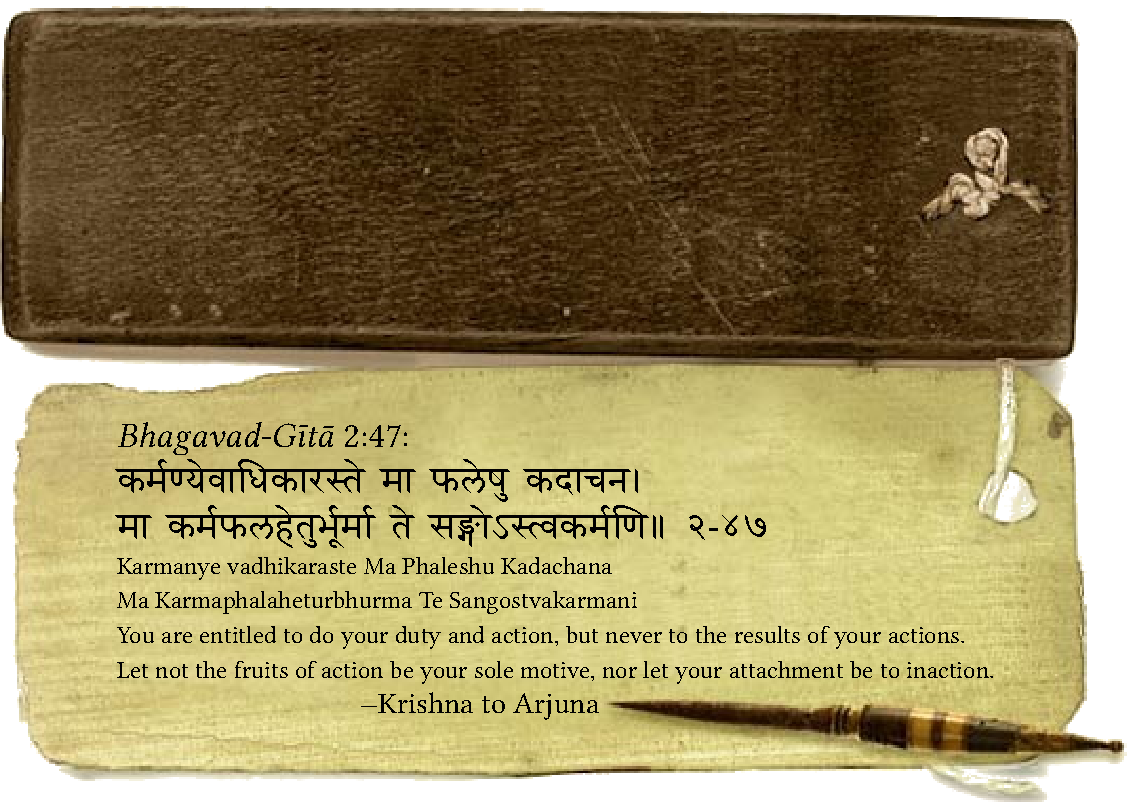
\includegraphics[width=0.85\textwidth]{narayam_sanskrit.png}
    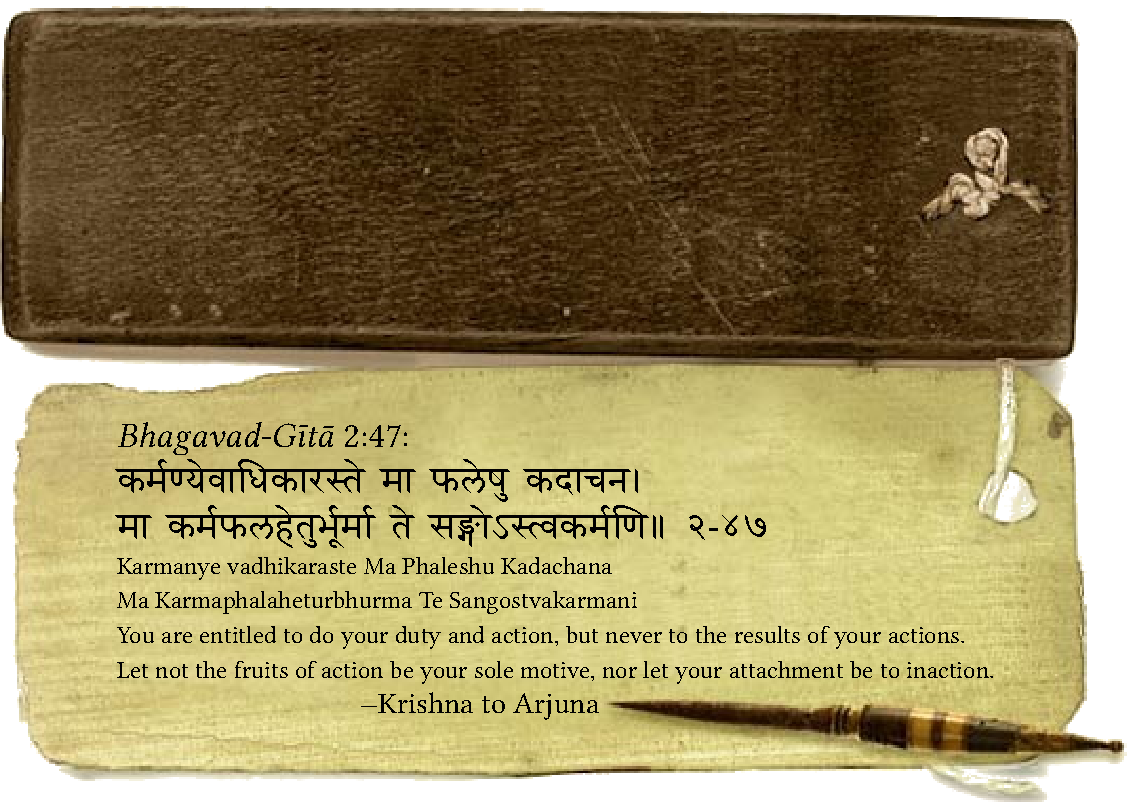
\includegraphics[width=0.85\textwidth]{narayam_sanskrit.pdf}
    \flushright{\scriptsize The image `Thaliyola.jpg' (on which the Gita verse
        is overlaid by this thesis author) was sourced from Wikimedia Commons and is licensed CC-BY-SA 2.5}

\end{minipage}
\endgroup

\setstretch{1.348361657291667} % golden-ratio stretch (1.2 x 1.348 = 1.618)
% Thesis Abstract -----------------------------------------------------

%\begin{abstractslong}    %uncommenting this line, gives a different abstract heading
\begin{abstracts}        %this creates the heading for the abstract page
\addcontentsline{toc}{chapter}{Abstract}
Put your abstract here...

\end{abstracts}


\cleardoublepage
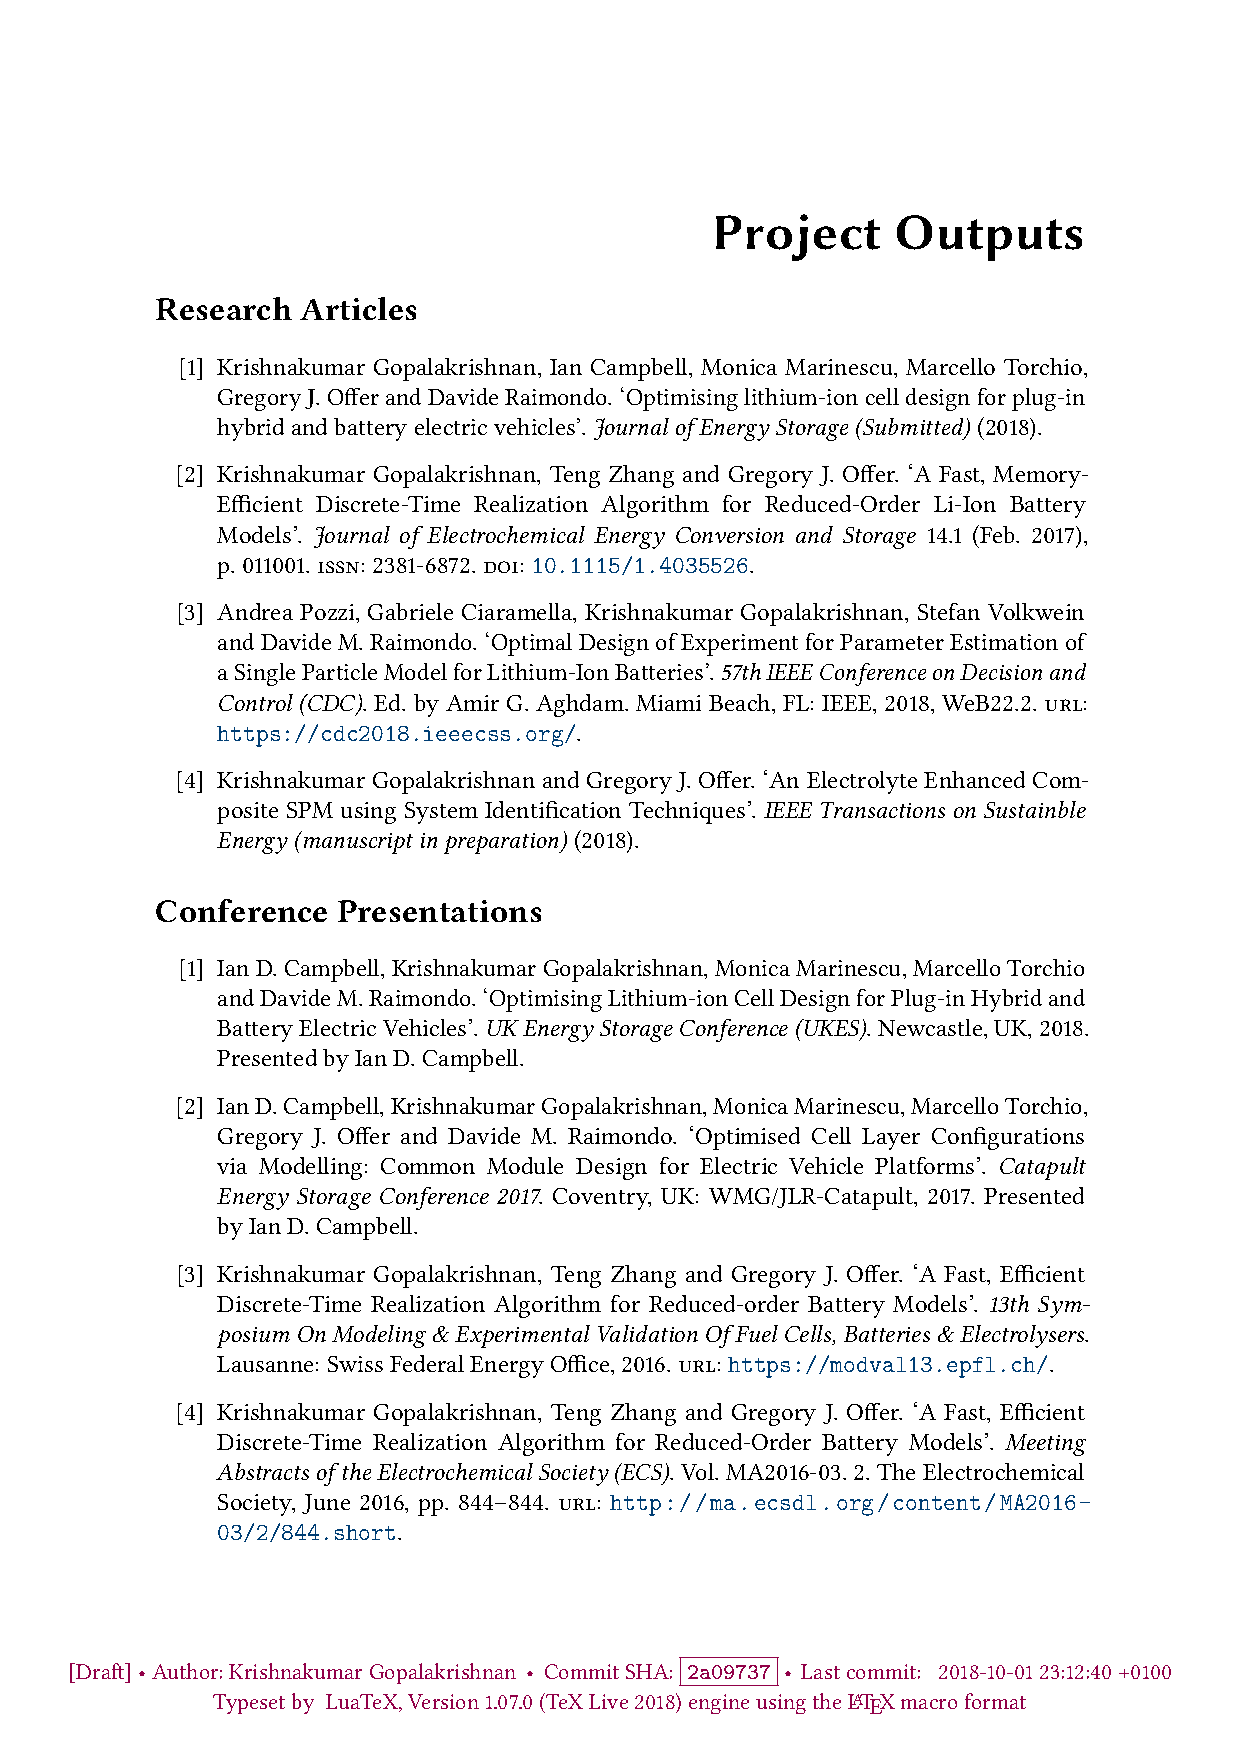
\includepdf[link, pages=-, pagecommand={\thispagestyle{plain}}]{project_outputs.pdf}
% \includepdf[pages=-, pagecommand={\thispagestyle{plain}}]{dedication_new.pdf}
\cleardoublepage

%: ----------------------- table of contents ------------------------
\renewcommand{\baselinestretch}{0.3}\normalsize
\cleardoublepage
\glsunsetall
\microtypesetup{protrusion=false} % disables protrusion locally in the document
\pdfbookmark[chapter]{\contentsname}{toc} % \pdfbookmark[<level>]{<title>}{<dest>} with bookmark package. https://tex.stackexchange.com/questions/65544/how-to-link-table-of-contents-in-thesis-pdf
\tableofcontents            % print the table of contents % \addtocontents{toc}{\protect{\pdfbookmark[1]{\contentsname}{toc}}} % https://tex.stackexchange.com/questions/1820/contents-in-pdf-bookmarks without bookmark package

%: ----------------------- list of figures/tables etc. ------------------------
\cleardoublepage
\setstretch{1.1} % 1.1 worked fine
\listoffigures
\cleardoublepage
\onehalfspacing
\listoftables
\cleardoublepage
% https://tex.stackexchange.com/questions/69184/remove-blank-page-between-list-of-figures-and-list-of-tables
{\addcontentsline{toc}{chapter}{List of Algorithms} \listofalgorithms \let\clearpage\relax \addcontentsline{toc}{chapter}{List of Program Code} \begingroup   \tcblistof[\chapter*]{mypyg}{List of Program Code} \endgroup}
\glsresetall
\setstretch{1.0} % for glossaries
\begingroup
\printglossary[type=acronym, title={List of Acronyms}, nonumberlist, style=super]\label{ch:glossary}
\endgroup
\microtypesetup{protrusion=true} % re-enables protrusion

% Required to maintain continuous arabic numbering
\makeatletter
\@mainmattertrue
\makeatother
\cleardoublepage

\setstretch{1.348361657291667} % golden-ratio stretch (1.2 x 1.348 = 1.618)
\setcounter{chapter}{0}
% -*- root: ../../main.tex -*-
%!TEX root = ../../main.tex
% vim:textwidth=80 fo=cqt

% \clearpage
\graphicspath{{chapters/introduction/figures/}}
\chapter{Introduction}\label{ch:intro}

% need a symbol Nomenclature

\capolettera{T}{ightening} emissions  regulations in various  industrial sectors
have led  to a renewed interest  in sustainable energy sources  in recent years.
In  particular,  the  burgeoning  demand  for  clean  energy  has  prompted  the
automotive and  consumer electronics industries  to explore advanced  methods of
energy storage~\cite{Weiss2011}. Li-ion batteries\footnote{The term(s) `cell(s)'
and  `battery(ies)' are  used interchangeably  in this  thesis. Technically,  an
electrochemical cell is the smallest  self-contained unit (housed in a packaging
with terminal connectors) that is capable of both storing and delivering energy.
A battery (also referred to as a battery  `pack') is made up of a group of cells
arranged  in  a  custom  configuration to  meet  certain  system-level  voltage,
current and  power demands.  The focal  point of  this thesis  is a  single cell
(a  discussion of  what  this  entails is  provided  shortly hereafter,  thereby
narrowing  down the  geometrical scope  of large  portions of  this thesis  to a
precisely defined unit). Scaling of various  quantities from the pack level down
to  the  cell  level  is  discussed  wherever  appropriate.}  are  seen  as  key
enablers  in this  quest due  to  the attractiveness  of their  high energy  and
power  densities compared  to  other competing  non-conventional energy  storage
technologies~\cite{Ibrahim2008}.  However, with  this  surge  in energy  storage
demands  comes  stricter  requirements  for  cell  longevity,  performance,  and
adhesion  to  safety  requirements,  particularly  for  adoption  in  mainstream
transport  electrification~\cite{Andrea2010}.  In  contrast to  other  incumbent
technologies,  lithium-ion cells  have several  advantages such  as high  energy
density,  long life-cycles,  low internal  resistance, low  self-discharge, long
cycle life,  fast charge  and discharge  cycles~\cite{Reddy2011,Plett2015}. This
makes them the preferred choice for storage and on-demand retrieval of energy in
modern consumer electronics and~\glspl{xeV}.

% Different type of cells - Prismatic,  pouch and cylindrical. How pouch cells are
% used in automotive industry acknowledge Tesla, but cite counter citations. Layer
% photos etc

% Precise definition of cell unit
% \section{Geomtery}
% C-rate definition

\section{Working Principle}\label{subsec:liionchemistry}

This section  provides a  brief overview of  the essential  chemistry principles
that  helps  to  describe the  working  principle  of  a  lithium ion  cell  and
represents the author's digested summary  of the introductory concepts presented
in Plett~\cite{Plett2015}.

\Cref{fig:chargetransferprocess} depicts the construction of one electrochemical
layer of a lithium ion cell. The positive electrode consists of porous particles
of  Lithium-Transition  Metal  Oxide  (MO)  compounds.  The  negative  electrode
typically employs some variant of microporous graphite. The porous nature of the
electrodes provide pathways for lithium  ion conduction through the electrolyte.
Due  to  the  special  construction  of the  electrode  structure,  there  exist
interstitial  sites  which act  as  intercalation  spots for  lithium  shuttling
between the two electrodes. The electrolyte, which floods the cell, helps in the
conduction of \ch{Li^+}~ions. The separator membrane allows the passage of these
ions  between  the  two  electrodes,  but  prevents  internal  short-circuit  by
inhibiting electronic  conduction through it. The  current collectors facilitate
passage of electrons generated during the charge transfer at particle surface to
the external circuit.

\begin{figure}[!htbp]
    \centering
    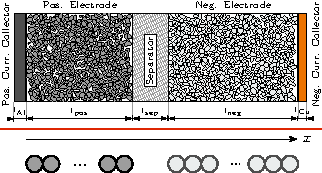
\includegraphics[width=\textwidth]{cropped_cell_sandwich_for_thesis}
    \caption[Illustration of a lithium ion cell]{Schematic depicting the basic construction of a lithium ion cell.}
    \label{fig:chargetransferprocess}
\end{figure}

At fully  charged condition,  the majority  of lithium in  the system  is stored
within the negative electrode  microstructure. During discharge, \ch{Li^0}~atoms
diffuse out of  deep interstitial sites towards the surface  of the particles in
the  negative  electrode.  At  the  surface  (electrode-electrolyte  interface),
a  charge-transfer  process  takes  place according  to  Butler-Volmer  kinetics
\cref{eq:butlervolmer},  leading   to  the   formation  of   \ch{Li^+}~ions  and
electrons. The electrons are passed to  the external circuit through the \ch{Cu}
current collectors  onto which  the conductive matrix  composed of  the negative
electrode material and binders is  coated. The \ch{Li^+}~ions travel through the
electrolyte phase,  crossing the  separator membrane  to the  positive electrode
where they  encounter an  electron influx  from the  external circuit.  A charge
transfer  reaction  takes  place  at  the  surface  of  the  positive  electrode
particles, leading to the formation of neutral \ch{Li^0}~atoms that diffuse into
the positive electrode microstructure.

During  the   charging  process,  the   reverse  phenomena  occur.   lithium  is
de-intercalated  from  the  positive  electrode and  a  similar  charge-transfer
happens  at  the surface,  leading  to  the  formation of  \ch{Li^+}~ions  which
reach  the  negative  electrode  by   passing  through  the  separator.  At  the
surface of  the negative electrode  particles, these ions absorb  electrons from
the  external  circuit,  leading  to the  formation  of  neutral~\ch{Li^0}  that
diffuses  into  interior  vacant  spaces  in  the  layered  graphite  electrode.
\Cref{eq:NegElectrodeRxn,eq:PosElectrodeRxn} summarise the  reactions during the
charging and discharging process at the surfaces of both electrode materials.
\begin{align}
    \ch{Li_{$x$} C                            &<=>[\tiny{discharge}][\tiny{charge}] C + $x$ Li^+ + $x$ e^-}\label{eq:NegElectrodeRxn}\\
    \ch{Li_{1-$x$} M O2 + $x$ Li^+  + $x$ e^- &<=>[\tiny{discharge}][\tiny{charge}] LiMO2}\label{eq:PosElectrodeRxn}
\end{align}
where    \ch{M}~represents    a    transition   metal    compound   such    as
\ch{Ni_{1/3}Co_{1/3}Mn_{1/3}}~(NMC),   \ch{Ni_{0.8}Co_{0.15}Al_{0.05}}~(NCA)
amongst other  choices~\cite{Reddy2011}. Assuming  no loss of  cycleable lithium
due to  parasitic side  reactions or  through other  mechanisms, the  process is
fully reversible.


The electrochemical potential at each electrode  is dependent upon the extent of
its  lithiation. An  empirical  relationship of  each  electrode's potential  as
a  function  of  its  stoichiometry  can be  obtained,  and  is  dependent  upon
the  specific design  and  material  properties of  each  active material  under
consideration. Finally, the \gls{ocv} of the cell is obtained by subtracting the
negative electrode potential from its positive electrode counterpart.


\section{Battery Modelling}

Through accurate model representations  of the electrochemical-thermal behaviour
of  the cell,  advanced monitoring  and control  strategies can  be deployed  to
tackle  the current  research  topics  in Li-ion  batteries  such as  increasing
cycle-life,  improving  operational   safety  and  performance~\cite{Plett2015}.
Over  the  past two  decades,  efforts  have  been  made to  construct  accurate
models  to  describe  the  physical, electrical,  thermal,  electrochemical  and
system-level performance of  Li-ion cells, leading to  modelling strategies with
various  levels of  sophistication. For  the interested  reader, the  article by
Grazioli~\etal~\cite{Grazioli2016a} provides  a broad introduction to  the topic
of computational  modelling of  lithium ion batteries.  Large in-roads  into the
depth of the modelling  art can be made by perusing  comprehensive books on this
topic such  as those by  Plett~\cite{Plett2015}, Hariharan~\cite{Hariharan2017},
and Rahn and Wang~\cite{Rahn2013}.

The  need  to  address  the  operational challenges  of  lithium  ion  batteries
in   an   embedded   environment   such  as   on-board   an   electric   vehicle
has   led   to  an   increased   impetus   on   the  development   of   advanced
\glspl{bms}~\cite{Bergveld2002}. In vehicular  applications, the only measurable
quantities  of  a  lithium  ion  cell are  its  terminal  voltage,  current  and
temperature. This implies  that several internal states of the  cell such as its
\gls{soc}, whose  real-time computation is  vital to the optimal  performance of
the cell, need to be estimated from these available measurements. Therefore, the
performance  of  a \gls{bms}  for  tasks  such  as  online state  estimation  is
dependent upon the  fidelity of the underlying cell  model. Sophisticated models
of  the  cell enable  these  quantities  to  be  estimated more  accurately  and
facilitate the implementation  of advanced control algorithms.  Therefore, it is
imperative  that  the cell  model  used  is suitable  for  being  embedded in  a
real-time \gls{bms}.

Most battery  models have the primary  goal of accurately predicting  the cell's
terminal  voltage  at each  time-step.  This  is so  that  the  output from  the
predictor routine  can be compared  to the  measured voltage and  the difference
between them  may be used in  a suitable corrector-subroutine to  improve future
prediction.  The combined  information from  the model  and measurement  is then
blended in a suitable way to estimate the cell's \gls{soc}.

More   advanced  models   strive   to  provide   insight   into  various   other
physico-chemical quantities  that could affect  the cell's health. The  field of
Li-ion battery modelling can be classified into two broad categories
---
\begin{enumerate*}[label=\roman*)]
    \item empirical/ad-hoc \glspl{ecm}, and
    \item detailed  \glspl{pbm} that are based  upon first principles.
\end{enumerate*}
A  comprehensive summary  of  various models  that  belong to  each  of the  two
categories  is  discussed  in Seaman~\etal~\cite{Seaman2014}.  A  characteristic
aspect that contrasts  them is the fact that they  are typically
at loggerheads with each other in terms of their computational complexity.

\subsection{\glsfmtlong{ecm}s}\label{subsec:ecms}

\glspl{ecm}  employ circuit  elements  such as  voltage  sources, resistors  and
capacitors to  model the behaviour  of batteries at their  electrical terminals.
The cell's  thermal subsystem may  also be  modelled by an  analogous electrical
circuit. The  parameters of the  circuit are  typically functions of  the cell's
current, \gls{soc} and  temperature. These can be incorporated as  a lookup table by
curve-fitting  the model  to experimental  data. Using  such equivalent  circuit
models, two simple methods are available to compute the cell's \gls{soc} ---
\begin{enumerate*}[label=\itshape\alph*\upshape)]
    \item by using manufacturer-supplied  lookup table or graph of \gls{ocv} versus \gls{soc}, and
    \item by numerically integrating the charge passed in and out of the cell over time (commonly referred to as coulomb counting).
\end{enumerate*}
Both methods are computationally  amenable for small-scale embedded applications
such as  consumer  electronics;  however,  neither  one is  robust  to  handle  the
stringent demands in performance imposed  by modern vehicular applications.

Advanced state estimation algorithms such  as nonlinear Kalman filters may still
be able to use \glspl{ecm} as the plant model and obtain reasonable estimates of
the  cell's  \gls{soc}~\cite{Plett2006,  Sun2011}. However,  the  usefulness  of
\glspl{ecm} is limited by the fact that their parameters are derived essentially
by a  curve-fitting process using a  standard set of training  data. Since these
models are  not based on  any physical phenomena,  their ability to  predict the
cell's general behaviour  is extremely poor especially when  subject to current
profiles well  outside their training  realm. Another important  disadvantage of
equivalent circuit  models is that they  do not allow insights  into the various
internal states of the cell.

\glspl{ecm}  of  lithium  ion  batteries   have  been  extensively  studied  and
are  widely  applied.  However,  the aforementioned  difficulties  render  their
reliability and  accuracy questionable,  especially under highly  demanding load
profiles  experienced by  the battery  packs in  \glspl{xeV}. The  boundaries of
their  performance have  been well-quantified  (see~\cite{Plett2015,Plett2016}).
Although  various estimation  and control  algorithms continue  to be  developed
around them, the  \glspl{ecm} themselves are no longer the  subject of extensive
research. Hence, this thesis does not discuss them further.

\subsection{\glsfmtlong{pbm}s}\label{subsec:pbms}

\glsreset{pbm}

\glspl{pbm} consist of  governing equations that construct a  realisation of the
behaviour of the cell based  upon electrochemical principles such as equilibrium
thermodynamics,  material  diffusion  and  reaction  kinetics.  The  fundamental
advantage  to this  modelling approach  is that  it is  possible to  compute the
evolution of  internal states of  the cell  for arbitrary current  profiles. The
difficulty with  the physics-based  modelling approach  lies with  obtaining the
values  of all  the physical,  geometric, electrochemical,  thermal and  kinetic
parameters  of the  cell. Usually,  these parameters  are closely  guarded trade
secrets by cell manufacturers.

In  some  cases, it  may  be  possible to  obtain  a  subset of  these  physical
parameters   by  dissecting   cells  in   an  inert   environment  followed   by
further  characterisation   using  specialised  lab  equipment.   For  instance,
Ecker~\etal~\cite{Ecker2015}   demonstrate   the    reverse-engineering   of   a
\SI{7.5}{\amphour} pouch  cell by Kokam  Ltd.\ in  order to obtain  its physical
parameters. Nevertheless,  this is a tedious  process and is feasible  only with
access  to  such sophisticated  lab  equipment.  Furthermore, the  results  from
these  experiments are  susceptible to  characterisation  errors as  well as  to
cell-to-cell variations due to production spread. Therefore, some form of system
identification  method needs  to  be employed  for estimating  the  rest of  the
physical  parameters required  for  a  \gls{pbm}. Furthermore,  it  is a  common
practice to  rely on published  data for the  values of certain  cell parameters
that do  not depend on physical  construction, especially for those  that remain
universally true for a particular Li-ion chemistry.

The challenges involved  in model parametrisation is a research  exercise of its
own merit and  is not addressed in  this thesis. A redeeming factor  is that the
task of  parametrisation is a  one-off problem that  appears early in  the model
deployment  stage,  after which  the  rewards  of  superior performance  of  the
\glspl{pbm} can be reaped. Once  the model parameters are available, \glspl{pbm}
can be used in  aiding a deeper understanding of the working of  the cell and in
answering research  questions that could  otherwise not be answered  with simple
\glspl{ecm}. One area  of focus of this  thesis is to broach  a less-probed area
--- exploring  the possibility  of using  a \gls{pbm}  for the  \emph{design} of
pouch  cells  used  in  automotive  applications which  shall  be  presented  in
\cref{ch:modelbaseddesign}.

A major disadvantage of \glspl{pbm} from an implementation point of view is that
solving for  the model's field  variables is time-consuming. In  particular, the
more  sophisticated  \glspl{pbm}  require  the use  of  multi-physics  \gls{pde}
solvers  and  hence  are  not  typically  suitable  for  embedded  applications.
Nevertheless,  for   high  performance   applications  such  as   in  automotive
\glspl{bms}  wherein   state-of-health  monitoring  is  crucial,   there  is  an
overwhelming  demand for  obtaining insight  into internal  cell variables.  For
instance, the real-time computation of surface concentration of \ch{Li^0} in the
solid particles enable the \gls{bms} to regulate  power flow into and out of the
cell to proactively avoid plating and degradation of the cell.

In view of this consideration, model  order reduction techniques are seen as key
enablers that facilitate in porting the first-principles based predictive powers
of \glspl{pbm}  into a  real-time microcontroller.  This thesis  shall therefore
have  a  strong  focus  on  both the  analysis  and  implementation  aspects  of
\glspl{rom}.

\section{The \glsfmtlong{dfn} model}\label{sec:dfnmodel}

Doyle,  Fuller and  Newman~\cite{Doyle1993,Fuller1994}  developed an  isothermal
physics-based  porous electrode  model of  the  cell capable  of describing  its
internal variables such as
\begin{enumerate*}[label=\itshape\alph*\upshape)]
    \item potential on the solid particles~$\phi_\text{s}$,
    \item potential in the electrolyte solution~$\phi_\text{e}$,
    \item concentration of \ch{Li^0} in the solid particles~$\c_\text{s}$,
    \item ionic concentration in the electrolyte solution~$\c_\text{e}$, and
    \item molar flux density of lithium at the solid-electrolyte boundary~$j$.
\end{enumerate*}
The most popular computational implementation  of the \gls{dfn} equations is the
\gls{p2d}  model~\cite{Plett2015}. In  the \gls{p2d}  implementation, all  field
variables  of  the  \gls{dfn}  model  are  computed  at  each  spatial  location
along  the axial  thickness of  the cell.  However, the  solid concentration  in
spherical electrode particles  is solved in a radial co-ordinate  system that is
perpendicular to  the axial  direction of  the cell's  thickness. The  axial and
radial dimensions are coupled at each  particle's surface through the molar flux
density  describing the  rate of  pore-wall flux  that crosses  from solid  into
electrolyte  or  vice-versa.  The  equations and  boundary  conditions  for  the
\gls{p2d} implementation of the \gls{dfn} model is shown in \cref{tbl:dfneqns}.

% -*- root: ../../main.tex -*-
%!TEX root = ../../main.tex
% this file is called up by main.tex
% content in this file will be fed into the main document
% vim:nospell textwidth=180 foldlevelstart=3 foldlevel=3 conceallevel=0

\begin{table}[!htbp]
    \centering
    \caption[Governing equations and boundary conditions of the \glsfmtshort{dfn} model]{Governing equations and boundary conditions of the \glsfirst{dfn} model cast in its
        \glsfirst{p2d} description. Apart from those equations whose sources are explicitly indicated with inline references, all equations of the \gls{dfn} model presented herein
        are obtained from the lecture notes by Plett~\cite{PlettECE5710_04}, suitably cast in their \gls{p2d} formulation. To maintain comptability with computer codes from the simulation tool~LIONSIMBA~\cite{Torchio2016}, the electrolyte potential at the positive electrode/current collector interface is set to zero (second boundary condition in \cref{eq:dfnliquidpotential})
    \ie{} chosen as the  ground reference.  The notation of symbols has been suitably adapted from the cited sources and is detailed in \nameref{symbols}~(see \cpageref{symbols}).}
    \label{tbl:dfneqns}
    \begingroup
    \makeatletter\def\f@size{9.65}\check@mathfonts
    \addtolength{\jot}{0.875em}
    \begin{tabular*}{\textwidth}{@{} l | c r l r @{}}
        \toprule
        \multicolumn{1}{c}{Region} & Governing equations & \multicolumn{2}{c}{Boundary conditions} & {} \\
        \midrule
        \multicolumn{1}{l |}{\rotatebox[origin=c]{+90}{\makecell{\scriptsize All regions, \scriptsize \muinnegseppos \\ \scriptsize Electrodes only, \scriptsize \lambdainnegpos}}} &
        $\begin{aligned} % placement: default is "center", options are "top" and "bottom"
            \vphantom{\diffp{c_\slambda}{r}{\mathrlap{r = R_\plambda}}}
            \diffp{c_\slambda}{t} &= \frac{D_\slambda}{r^2}\diffp{}{r}\left(r^2 \diffp{c_\slambda}{r} \right) \\
            \vphantom{\diffp{c_\text{e}}{x}{\mathrlap{x = l_\text{tot}}}}
            \varepsilon_\mu \diffp{c_\text{e}}{t} &= \diffp{}{x}\left(D_\effmu \diffp{c_\text{e}}{x} \right) + (1 - t^0_\text{+}) a_\slambda j_\lambda \\
            \vphantom{\diffp{\phi_\text{e}}{x}{\mathrlap{x = 0}}} {-a_\slambda F j_\lambda} &= \diffp{}{x}\left(\kappa_\effmu \diffp{\phi_\text{e}}{x}\right) + \diffp{}{x}\left(\kappa_\effmu \frac{2 R T(t)}{F} (t^0_{+}-1)\diffp{ \ln c_\text{e}}{x}\right) \\
            \vphantom{\diffp{\phi_\slambda}{x}{\mathrlap{\substack{x = x_\text{pos/sep}\\x = x_\text{neg/sep}}}}} a_\slambda F j_\lambda &= \diffp{}{x}\left(\sigma_\efflambda \diffp{\phi_\slambda}{x}\right) \\
            j_\lambda &= 2 k_\refflambda \sqrt{c_\text{e}\left(c_\slambdamax - c_\slambdasurf\right) c_\slambdasurf} \sinh \left(\frac{0.5 F}{R T(t)} \eta_\lambda \right)
        \end{aligned}$ &
        $\begin{aligned}
            \vphantom{\diffp{c_\slambda}{r}{\mathrlap{r = R_\plambda}}} \diffp{c_\slambda}{r}{\mathrlap{r = 0}}\hspace{1mm} &= 0, \\
            \vphantom{\diffp{c_\text{e}}{x}{\mathrlap{x = l_\text{tot}}}} \diffp{c_\text{e}}{x}{\mathrlap{x = 0}}\hspace{1mm} &= 0, \\
            \diffp{\phi_\text{e}}{x}{\mathrlap{x = 0}}\hspace{1mm} &= 0, \\
            \quad\diffp{\phi_\slambda}{x}{\mathrlap{\substack{x = x_\text{neg/sep}\\x = x_\text{sep/pos}}}}\hspace{1mm} &= 0, \\
            \vphantom{j_\lambda = 2 k_\lambdar \sqrt{c_\text{e}\left(c_\slambdamax - c_\slambdasurf\right) c_\slambdasurf} \sinh \left(\frac{0.5 F}{R T(t)} \eta_\lambda \right)}
            {}&\xdash[1.25em]{}
        \end{aligned}$ &
        $\begin{aligned}
            \diffp{c_\slambda}{r}{\mathrlap{r = R_\plambda}}\hspace{1mm} &= \frac{-j_\lambda}{D_\slambda} \\
            \diffp{c_\text{e}}{x}{\mathrlap{x = l_\text{tot}}}\hspace{1mm} &= 0 \\
        \vphantom{\diffp{\phi_\text{e}}{x}{\mathrlap{x = 0}}} \phi_\text{e}\Bigr\rvert_{\mathrlap{x=l_\text{tot}}} \hspace{1mm}&= 0 \\
        \vphantom{\diffp{\phi_\slambda}{x}{\mathrlap{\substack{x = x_\text{pos/sep}\\x = x_\text{neg/sep}}}}}
        \!\!\!\!\!\!\diffp{\phi_\slambda}{x}{\mathrlap{\substack{\!\!\!\!\!x=0\\x=x_\text{tot}}}}\hspace{1mm} &= \frac{- I}{\sigma_\efflambda A} \\
        \vphantom{j_\lambda = 2 k_\lambdar \sqrt{c_\text{e}\left(c_\slambdamax - c_\slambdasurf\right) c_\slambdasurf} \sinh \left(\frac{0.5 F}{R T(t)} \eta_\lambda \right)}
        {}&\xdash[1.25em]{}
    \end{aligned}$ &
    $\begin{aligned}
        \vphantom{\diffp{c_\slambda}{r}{\mathrlap{r = R_\plambda}}}\refstepcounter{equation}(\theequation)\label{eq:dfnsoliddiff} \\
        \vphantom{\diffp{c_\text{e}}{x}{\mathrlap{x = l_\text{tot}}}} \refstepcounter{equation}(\theequation)\label{eq:dfnliquiddiff} \\
        \vphantom{\diffp{\phi_\text{e}}{x}{\mathrlap{x = 0}}} \refstepcounter{equation}(\theequation) \label{eq:dfnliquidpotential}\\
        \vphantom{\diffp{\phi_\slambda}{x}{\mathrlap{\substack{x = x_\text{pos/sep}\\x = x_\text{neg/sep}}}}} \refstepcounter{equation}(\theequation) \label{eq:solidchargeconserve}\\
        \vphantom{j_\lambda = 2 k_\lambdar \sqrt{c_\text{e}\left(c_\slambdamax - c_\slambdasurf\right) c_\slambdasurf} \sinh \left(\frac{0.5 F}{R T(t)} \eta_\lambda \right)} \refstepcounter{equation}(\theequation)\label{eq:butlervolmer} \\
    \end{aligned}$ \\
    \bottomrule
\end{tabular*}
\endgroup
\begin{minipage}{\textwidth}
    \bigskip
    \begin{flushleft}
        \raggedright
        \makeatletter\def\f@size{12}\check@mathfonts
        $ \text{\textbullet{} } c_\text{e}  \coloneqq c_\text{e}(x,t),\, \phi_\text{e} \coloneqq \phi_\text{e}(x,t) \quad \big\{\, x \in [0,l_\text{tot}],\, (x=0)\symbol{"2259} \text{\footnotesize neg/Cucc},\, (x=l_\text{tot})\symbol{"2259} \text{\footnotesize pos/Alcc}\, \big\}$
        \\[0.9em]
        {\raggedright \small \uline{\lambdainnegpos}}
        $\begin{alignedat}{2}
            & \text{\textbullet{} } c_\slambda & & \coloneqq c_\slambda(r,t),\, c_\slambdasurf \coloneqq c_\slambda(r=R_\plambda,t) \quad \big\{\, r \in [0,R_\plambda],\, (r=0)\symbol{"2259} \text{\footnotesize center},\, (r=R_\plambda)\symbol{"2259} \text{\footnotesize surface}\, \big\} \\[0.9em]
            % & \text{\textbullet{} } c_\slambdasurf & & \coloneqq c_\slambda(r=R_\plambda,t)\\
            & \text{\textbullet{} } \phi_\slambda & & \coloneqq \phi_\slambda(x_\lambda,t),\, j_\lambda \coloneqq j_\lambda(x_\lambda,t) \quad \big\{\, x_\lambda \subset x, \, x_\text{neg} \in [0,l_\text{pos}],\, x_\text{pos} \in [l_{\text{pos}+\text{neg}},l_\text{tot}]\, \big\} \\[0.9em]
            & \text{\textbullet{} } \eta_\lambda & & \coloneqq \eta_\lambda(x,t) = \phi_\slambda(x,t) - \phi_\text{e}(x,t) - \mathcal{U}_\lambda(c_\slambdasurf) \\
            & \text{\textbullet{} } \sigma_\efflambda & & = \sigma_\lambda \varepsilon_\slambda,\, D_\sefflambda = D_\slambda
            e^{\frac{-E_{\text{a},D_\slambda}}{R}\left(\frac{1}{T(t)} - \frac{1}{T_\text{sink}}\right)},\, k_\refflambda = k_\lambdar
            e^{\frac{-E_{\text{a},k_\lambdar}}{R}\left(\frac{1}{T(t)} - \frac{1}{T_\text{sink}}\right)} \! \cdots \! \cdots \!  \text{(\footnotesize Torchio~\etal~\cite{Torchio2016}\normalsize)} \\[0.9em]
        \end{alignedat}$
        {\raggedright \small \uline{\muinnegseppos}}\\[0.5ex]
        $\begin{alignedat}{2}
            & \text{\textbullet{} } D_\effmu & & = D \varepsilon_\mu^{\text{brugg}_\mu} \\
            & \text{\textbullet{} } D & & \coloneqq D(\scriptstyle{c_\text{e},T}\,\textstyle) = 10^{-4} \times 10^{-4.43 - \frac{54}{T(t) - 229 - 5\times10^{-3} c_\text{e}(x,t)} -
            0.22\times10^{-3} c_\text{e}(x,t)} \mkern-2mu \cdots \! \cdots \! \cdots \! \cdots \! \cdots \! \cdots \! \cdots \!  \text{(\footnotesize Torchio~\etal~\cite{Torchio2016}\normalsize)} \\
        \end{alignedat}$
        \\
        \makeatletter\def\f@size{14}\check@mathfonts
        $\begin{alignedat}{2}
            & \text{\textbullet{} } \kappa_\effmu & & = \kappa \varepsilon_\mu^{\text{brugg}_\mu} \\
            & \text{\textbullet{} } \kappa & & \coloneqq \kappa\scriptstyle{(c_\text{e},T)}\; = \; \parbox[t]{11.60cm}{$\scriptstyle 10^{-4} \times c_\text{e}(x,t)\Big(-10.5 +
            0.668\times10^{-3} c_\text{e}(x,t) + 0.494\times10^{-6} c_\text{e}^2(x,t) + \big(0.074 - 1.78\times10^{-5}c_\text{e}(x,t)$ \\  $\scriptstyle
    -8.86\times10^{-10}c_\text{e}^2(x,t)\big)T(t) + \big(-6.96\times10^{-5} + 2.8\times10^{-8} c_\text{e}(x,t)\big)T^2(t)\Big)^2 \kern-1pt \cdots \cdots \cdots \cdots \text{(\footnotesize Torchio~\etal~\cite{Torchio2016}\normalsize)}$}  \\
        \end{alignedat}$
    \end{flushleft}
\end{minipage}
\end{table}

\clearpage


In  this  thesis,  this  \gls{p2d}  implementation of  the  \gls{dfn}  model  is
considered as  the reference (and  only) \gls{pbm}. Although  thermal dependence
of  parameters  such  as  electrolyte  conductivity  and  diffusivity  is  shown
in \cref{tbl:dfneqns}, a sophisticated description  of detailed thermal dynamics
\ie~a description  of spatio-temporal evolution of cell's  temperature using a
set of ordinary/partial  differential equations is not considered  in this work.

For those aspects of this thesis dealing with the analysis and implementation of
various  \glspl{rom} and  the  improvements  imparted herein  to  them, only  an
\emph{isothermal}  implementation  (at  \SI{298.15}{\kelvin}) of  the  \gls{p2d}
equations  is  considered.  The  performance  of  the  various  \glspl{rom}  are
compared  against this  reference benchmark.  In consideration  of the  relative
sparsity of  such detailed analysis  of \glspl{rom} in existing  literature (see
\cref{ch:littreview}),  the  author  of  this  thesis  considers  that  such  an
analysis, albeit isothermal, is  the need of the hour and  is imperative to gain
a  deeper  understanding  of  the  performance  boundaries  of  various  popular
\glspl{rom}.

% Further  extensions to  the  analysis  presented here  to  include various thermal effects can be considered for future research.

Since temperature  plays a crucial  role in the  operation of cells  and battery
packs in \glspl{xeV},  an isothermal model is unsuitable for  design purposes. A
model-based design that does not consider thermal effects is likely to stray far
from the operating regimen and fail  spectacularly. On the other hand, including
a sophisticated thermally coupled model  is unlikely to yield significant gains.
Firstly, running  fully coupled electrochemical-thermal model  based simulations
over the entire design space  is computationally expensive. Secondly, the design
results  of the  model have  to  be anyway  verified using  a reasonable  number
of  experimental prototypes.  Taking  into account  these  considerations it  is
deemed  that, for  the design  aspect  of this  thesis, a  lumped thermal  model
suffices.  This  simplified thermal  model  is  bidirectionally coupled  to  the
\gls{p2d} equations  (see \cref{tbl:dfneqns})  of the electrochemical  model and
is  used as  the  \gls{pbm}  underpinning the  model-based  design discussed  in
\cref{ch:modelbaseddesign}.

The rest of the thesis is organised as follows. \Cref{ch:littreview} presents an
overview of pertinent modelling art.  The literature on model-based design shall
be  evaluated  here and  the  present  shortcomings  identified. The  survey  of
literature  also  considers the  advancements  in  the  field of  reduced  order
modelling from  their analysis and implementation  perspectives. A computational
framework  for  optimising the  number  of  layers  within an  automotive  pouch
cell  is  presented  in  \cref{ch:modelbaseddesign}.  In  \cref{ch:improveddra},
the  computational   bottlenecks  in   a  specific  \gls{rom}   method  \viz~the
\gls{dra} is  analysed in  detail and  an improved  alternative is  proposed. In
\Cref{ch:spmanalysis},  the simplest  time-domain  \gls{pbm},  the \gls{spm}  is
introduced and  its performance  is analysed. Salient  advancements made  to the
basic \gls{spm} in the literature  are presented and their shortcoming analysed.
A discrete-time formulation focusing on  the numerical implementation aspects is
also  presented. In  \cref{ch:newelectrolytemodel},  the causal  factor for  the
lacklustre performance of  a state of the art  electrolyte-enhanced \gls{spm} is
unearthed. \Cref{ch:newelectrolytemodel}  also proposes a new  electrolyte model
which represents a novel application  of the system identification technique and
the  superior performance  of  this composite  model  is demonstrated.  Finally,
\cref{ch:conclusions} highlights the salient conclusions  that can be drawn from
the findings presented in  this thesis and paves the way  for future research by
identifying key unsolved tasks in physics-based battery modelling.

% need a symbol Nomenclature

% \subsection{Organisation of Thesis}

% nice figure here (with Bohr model of atom)
% \Cref{ch:improveddra} analyses a critical weakness in a sophisticated \gls{rom}
% and proposes a numerical method to circumvent it.
% different \glspl{rom} shall be performed in

% \cite{Seaman2014} provide a comprehensive survey  of the wide range of battery
% models out there.

% This  thesis  strives to  represent  all  physical  quantities in  the  standard
% International  System  of Units  (SI-Units).  However,  there are  some  notable
% exceptions \eg~for the capacity of a  Li-ion cell, which is represented in the
% practical units  of Ampere  hours (\SI{}Ah),  rather than the  base SI  Units of
% Coulombs (\SI{}{\coulomb}).  Such exceptions  are made  taking into  account the
% prevalent conventions in standard literature.

% \fxnote{Where does  this paragraph go? End  of this section/end of  chapter or
% even  last  chapter?}  The  identification of  individual  parameters  of  the
% \gls{dfn} model  remains a  key area  in battery  modelling that  remains only
% partially  explored. Nevertheless,  this effort  is critical  to ensure  rapid
% adoption  of any  physics-based  model and  sophisticated control  algorithms.
% The  state of  the  art in  this  area, the  challenges  involved and  current
% efforts  in  this  direction are  explored  in \cref{ch:futurework}.  Although
% sensitivity  analysis  of  the  \gls{dfn} parameters  has  been  performed  in
% literature, \fxnote{citation here} the extent to which parameter uncertainties
% influence  the   numerical  values  in  the   $A,  B,  C$  and   $D$  matrices
% of \cref{eq:LTIstatespace} has not yet been attempted. In continuation of this
% research aspect, the order of magnitude  shift in eigen/singular values of the
% relevant system matrix also need to be quantified to enable an informed choice
% about stability of such models for real-time implementations.

% need a symbol Nomenclature
 % Introduction
\setcounter{chapter}{1}
 % -*- root: ../../main.tex -*-
% !TEX root = ../../main.tex
% this file is called up by main.tex
% content in this file will be fed into the main document
% vim:textwidth=80 fo=cqt


\graphicspath{{chapters/litt_review/figures/}}
% ----------------------- contents from here ------------------------

\clearpage
\chapter{Review of Literature}\label{ch:littreview}
\vspace*{-10mm}
\startcontents[chapters]
\printcontents[chapters]{}{1}{\setcounter{tocdepth}{1}}

\bigskip
% \vspace*{\fill}
% -*- root: ../../main.tex -*-
%!TEX root = ../../main.tex
% this file is called up by main.tex
% content in this file will be fed into the main document
% vim:textwidth=80 fo=cqt

\capolettera{T}{his} chapter  discusses the  state of  the art  in the  field of
lithium ion battery modelling pertinent  to the research sub-topics discussed in
this thesis.   The modelling  art is  therefore presented in three  parts, each
providing a critical review of
\begin{enumerate}[label=\itshape\alph*\upshape), topsep=0pt, itemsep=0pt, before={\vspace*{-0.25\baselineskip}}]
    \item the body of literature discussing model-based design of lithium ion cells.
    \item prior works dealing with the analysis and implementation aspects
        of reduced order modelling of lithium ion cells, whose revelations lead
        to a focus on
    \item publications discussing the \gls{spm} and its variants.
\end{enumerate}



\section{Model Based Design for Batteries: Overview of Prior Art}\label{sec:modelbasedliterature}
% -*- root: ../../main.tex -*-
%!TEX root = ../../main.tex
% vim:textwidth=80 fo=cqt

% As discussed  in \cref{ch:intro},  there is  a growing  need to  replace replace
% fossil  fuel-based  vehicles  with   cleaner  alternatives  wherein  Lithium-ion
% batteries hold  much promise.  The next generation  of battery  powered vehicles
% shall  require  higher  energy  density  batteries  without  compromising  power
% density. Furthermore,  the costs of the  on-board battery pack shall  have to be
% considerably lowered.

% Researchers in the field have aimed to bring about improvements to the incumbent
% lithium ion battery technology by focussing on various aspects.

% Modifications are  attempted  through various  approaches i)  through
% fundamental material advances [  2 , 3 ], ii) new chemistries [  4 ], iii) novel
% cell designs and  manufacturing techniques [ 5 ], iv)  system design or reducing
% the costs of assembly [ 6 , 7  ], and v) improved controller design for advanced
% battery management systems [8].

In sharp contrast to the cornucopia of published literature dealing with reduced
order  modelling  of cells  (see  \cref{sec:classificationscheme}),  there is  a
relative paucity of prior art that discuss model-based cell design. This section
aims to critically evaluate this sparse pool of knowledge.

At  the  outset, it  is  important  to clarify  this  thesis  author's views  on
model-based design in general and why this topic was chosen as an aspect of this
thesis.  In  the  recent  decades,  industries  pertaining  to  different  walks
of  life,  cutting  across  any  one  discipline,  have  begun  to  establish  a
model-led product/process development culture. For instance, a broad overview of
industrial  research  policy by  Thomke~\cite{Thomke1998}  towards  the turn  of
the  last millennium  provides  quantifiable evidence  that  a simulation  based
design approach  in the  automotive industry  has had a  positive impact  in the
crash-worthiness of resulting  vehicular designs. At a high  level, the benefits
of any model-based design are ---
\begin{enumerate*}[label=\itshape\alph*\upshape)]
    \item reducing the number of design iterations thereby speeding up the time to a production-ready prototype, and
    \item improved understanding of the variables influencing design gained by formalising empirical/ad-hoc knowledge.
\end{enumerate*}
Finally, it is a well-known fact that, computer-time is cheaper than human time.
Therefore, with  a simulation-oriented design  approach, it is often  cheaper to
explore Monte~Carlo-like design scenarios  using a computer model than iterating
over  a  series  of  rudimentary  prototypes  in  the  lab.  Finally,  once  the
results  predicted by  the model  has stabilised  enough to  satisfy the  design
specifications,  prototyping can  be  attempted, thereby  reducing  the time  to
market.

The   aforementioned    views   of    the   thesis    author   is    echoed   by
Becker~\etal~\cite{Becker2005}  who  present  a   persuasive  view  that,  since
it  becomes  essential  to  have   a  deeper  understanding  of  the  simulation
tools  to successfully  employ a  model-led  design, this  can trigger  sweeping
changes percolating  into the  very core  of the  problem-solving culture  in an
organisation. Although relatively  at its infancy when it comes  to cell design,
model-based  designs have  been applied  at the  pack-level in  the past  and is
therefore not a  newcomer to the battery  industry in general. In  the middle of
the last  decade, a clarion  call to the industry  to adopt simulation  tools in
battery  engineering was  issued  by Spotnitz~\cite{Spotnitz2005}.  In the  said
article,  the author  questioned  the anachronistic  industry  trend of  relying
heavily on `making and testing' rather than aiming to understand the fundamental
governing equations  and principles  of a  battery and  using this  know-how for
design. Spotnitz~\cite{Spotnitz2005}  further argues  that using  \glspl{pbm} of
batteries could provide  reliable understanding of their behaviour,  and that as
the  understanding of  the  community steadily  grows, it  could  bring about  a
significant speed-up of battery development.

The nature and  scope of `model-based design' as intended  by this thesis author
needs to  be clarified. Since  this thesis focuses exclusively  on physics-based
modelling, the term  `model' pertains to \glsfirst{pbm}s and  not \glspl{ecm} or
any  other type  of  battery  models (such  as  other empirical/ad-hoc  models).
Therefore, the  survey of literature  here does  not include any  design efforts
outside of this scope.

There is  evidence that  computational modelling has  been successfully  used to
facilitate the development of novel energy storage materials. The review article
by Islam and Fisher~\cite{Islam2014} provides an overview of the use of computer
simulation  into  gaining  a  deeper  insight into  the  working  of  new  types
of  cathode  materials.  The  computer  models referred  to  in  this  work  are
not  volume-averaged models  at the  cell-level, but  detailed ab-initio  models
constructed using techniques  such as Density Functional  Theory~(DFT). While it
is heartening  to see  such a comprehensive  review of  computational techniques
applied to energy  storage, there are two distinct reasons  why the art reviewed
therein does  not align  with the goals  of this thesis.  Firstly, in  the works
reviewed in the  said article, computer simulation is used  primarily to aid the
understanding needed to develop next generation of energy storage components and
\emph{not} as a design tool. Secondly, this article uses computational modelling
to study  structural properties  at the  meso and nano  scales. While  these are
of  utmost importance  to  researchers involved  in  synthesising prototypes  of
next  generation  of energy  storage  materials,  they  are not  applicable  for
production-ready cell-designs at scale. Since this  thesis has a strong focus on
providing readily  applicable solutions  to industry  for incumbent  lithium ion
chemistries,  there is  no motivation  to pursue  the methods  discussed in  the
aforementioned work for the design aspects of this thesis.




\section{Reduced Order Models: A New Classification Scheme}\label{sec:classificationscheme}
% -*- root: ../../main.tex -*-
%!TEX root = ../../main.tex
% vim:textwidth=80 fo=cqt

\glsreset{rom}

Battery modellers face the classic  conundrum of conjuring physics-based battery
models that remain amenable for control  applications. The prior attempts by the
research  community  to  tackle  this  challenge  is  examined  here.  The  term
`control-oriented model' can  be considered synonymous with  the term \gls{rom}.
This is due  to the fact that the inherent  complexity of \glspl{pbm} inherently
necessitates the  use of  some order  reduction strategy  for their  adoption in
control and  real-time applications. In this  thesis as well as  in the relevant
literature discussed here, these two terms have been used interchangeably.

Research into  \glspl{rom} is  motivated by  the pressing  need for  a real-time
model  with accuracy  properties of  full-order \glspl{pbm}  but possessing  the
computational  simplicity of  equivalent-circuit models  (see \cref{subsec:ecms}
and \cref{subsec:pbms}  for an overview). A  number of approaches to  reduce the
computational complexity  of the \glspl{pbm}  have been explored  in literature.
Jokar~\etal~\cite{Jokar2016}  provide  a  comprehensive review  of  the  various
categories of reduced order \glspl{pbm} for lithium ion batteries. However, this
work  does  not aim  to  classify  models  based on  time-vs-frequency  domains.
Fan~\etal{}~\cite{Fan2015}  conducted  a  review   of  reduced  order  modelling
methods, but only provide a generic overview of deriving and implementing models
in these  dual domains  without an  expository analysis  of the  implications of
these modelling  choices. Unlike  Jokar~\etal~\cite{Jokar2016}, this  review did
not aim to provide a classification of various reduced order models, but instead
emphasises  on  a broad  survey  of  relevant  methodologies and  tools  towards
\emph{obtaining} them.  Hence, neither  of these works  provide an  insight into
the  rubrics and  implications  of the  choice  of either  of  these domains  to
underpin  the  \glspl{rom}. Although  in  principle  the transformation  between
them  is  often  a straightforward  mathematical  exercise,  \fxnote{citation(s)
needed?}availability of models for final  implementation in the time domain aids
immediate uptake by  industry for adoption in online  \glspl{bms}. The treatment
of \gls{rom} from  this aspect is so  germane to the central  hypothesis of this
chapter,\fxnote{``can a simple time domain model  do the job?''} that the author
of this thesis feels compelled to undertake a simpler classification exercise of
the existing modelling  art, within the context of their  suitability for online
implementation.


In this discussion,  various modelling methodologies and  their resultant models
are viewed as  a single continuum. Consequently this thesis  discusses them from
such a  unified perspective without  microscopic separation of the  final models
from their progenitor mathematical methods. Furthermore, there is also a need to
highlight the salient works among the more recent advances and extensions to the
then  prevailing models  to obtain  an updated  view of  the modelling  art that
have  gained  traction  since the  publication  of  Jokar~\etal~\cite{Jokar2016}
and  Fan~\etal~\cite{Fan2015}. Hence,  the specialised  review of  reduced order
modelling  literature covered  in this  section  intends to  supplement ---  not
supplant --- the breadth of research covered between these works. In particular,
care has been taken to minimize repetition of background art already analysed in
these aforementioned review  articles, thereby striving to report  the subset of
prior research  that is  pertinent to illustrate  the new  classification scheme
introduced  here.  The  author  does  not  aim  to  adhere  to  a  chronological
presentation of such  background works. Instead, salient  \gls{rom} families are
usually  introduced in  the context  of discussing  their significance  within a
particular mathematical modelling technique.


In the views of this thesis author, physics-based control-oriented models can be
classified as belonging to one of the following categories:
\begin{itemize}
    \item Frequency domain \glsfmtshort{rom}s
    \item Quasi-hybrid time/frequency domain \glsfmtshort{rom}s
    \item Hybrid \glsfmtshort{rom}s based on equivalent circuits
    \item Time-domain \glsfmtshort{rom}s
\end{itemize}
It is important to distinguish between those models that are derived directly in
the time  domain versus  those that  are derived first  in the  frequency domain
and  later  converted  to  time  domain.  \fxnote{enumerate  all  the  desirable
characteristics and criterion upon which models are to be evaluated}


In  principle, any  modelling  method  that yields  a  time domain  mathematical
description of physical  phenomena that is lower in  computational complexity by
an  arbitrary magnitude  than the  original  \gls{dfn} model  can be  considered
as  a  candidate for  further  investigation.  In  the  absence of  a  canonical
or  quantitative definition  of  what  constitutes a  reduced  order model,  the
number of  candidate family of  models to  consider is overwhelmingly  large. In
practice, the  constraints and  challenges imposed  by the  scope of  this work,
\viz~suitability for  real-time implementation,  limits the choice  of candidate
modelling  families.  For  instance,   models  relying  primarily  on  classical
finite  difference~\cite{Smith2006}, Galerkin's  approximation~\cite{Dao2012} or
Galerkin's  projection~\cite{Fan2016,Fan2018}  methods  for  transformation  and
order  reduction of  one or  more  field variables  of the  \gls{dfn} model  are
excluded from  further study. This  is done in  view of the  impracticability of
implementing  such  models in  a  resource-constrained  environment such  as  an
embedded \gls{bms} controller.

\subsection{Frequency   domain   \glsfmtshort{rom}s}\label{subsec:freqdomainroms}

Owing  to the  low entry-barrier  for adoption  in a  real-time controller  that
typically  logs data  samples at  specific time  intervals, this  thesis focuses
exclusively on models that are cast in a mathematical form directly suitable for
final implementation  in the time domain.  This choice implies the  exclusion of
those models that are derived and  implemented entirely in the frequency domain.
For the sake  of readers interested in frequency domain  methods, the discussion
here  briefly introduces  salient literature  employing the  Padé approximation
method that serves as a backbone of a wide variety of frequency domain models.


The     transfer     function     oriented    Padé     approximation     method
for    low    order    physics-based     battery    modelling    pioneered    by
Forman~\etal{}~\cite{Forman2011a}    has   gained    widespread   adoption    in
the    areas     of    cell     design~\cite{Marcicki2013},    charge-trajectory
optimisation~\cite{Bashash2010},    controller    design~\cite{Perez2015}    and
state    estimation~\cite{Marcicki2013,Moura2012}.     Although    Prasad    and
Rahn~\cite{Prasad2013} present  an online identification  of a subset  of ageing
parameters  using  a  Padé  model  and a  recursive  least  squares  algorithm,
specific  implementation  details  such  as  the  transformation  of  the  Padé
reduced  impedance  to discrete-time  difference  equations  were not  provided.
Padé  models  are  typically  limited  to offline  applications  owing  to  the
aggressive  trade-offs required  in its  approximation order  so as  to maintain
high  accuracies.  Those  models  truncated  to very  low  Padé  order  exhibit
poor  fidelity  and   perform  no  better  than   classical  equivalent  circuit
models,  although  recent  research  attempts have  focussed  to  mitigate  this
drawback~\cite{Yuan2017a,Yuan2017}.\fxnote{Should I  discuss how  they mitigated
this?}


\subsection{Quasi-hybrid time/frequency domain \glsfmtshort{rom}s}

Smith~\etal{}~\cite{Smith2007} pioneered a semi-hybrid approach to reduced order
modelling and  obtained closed  form expressions  for all  electrochemical field
variables  in  the frequency  domain  except  for those  describing  electrolyte
concentration and  potential (which were  solved separately using  the classical
finite difference discretisation method). To the author's knowledge, this is the
earliest published  instance wherein all  the dynamics  of the full  order model
were completely retained  in the frequency domain. This  was facilitated through
the use of  transcendental transfer functions that helped to  avoid the accuracy
degradation brought about by truncation  techniques such as Padé approximation.
In the first  stage of the model  derivation detailed in this  work, a composite
impedance model for the frequency range of interest from \SIrange{0}{10}{\hertz}
was  obtained.  This was  then  converted  to  a \engordnumber{12}  order  state
space  model using  the technique  of residue  grouping and  truncation, thereby
demonstrating the first instance of the so-called hybrid modelling workflow. The
\gls{rom} derived  in Smith~\etal{}~\cite{Smith2007}  was capable  of predicting
the cell's terminal voltage within  \SI{1}{\percent} of the full-order \gls{dfn}
model.

The  modelling  effort by  Smith~\etal{}~\cite{Smith2007}  also  has the  unique
distinction of  being the first  of its kind  to render a  physics-based battery
model  suitable  for  implementation  in  the  classical  \gls{lti}  state-space
formulation
\begin{equation}\label{eq:LTIstatespace}
    % \SwapAboveDisplaySkip
    \begin{aligned}
        \dot{\mathbf{x}} &= A\,\mathbf{x} + B\,\mathbf{u} \\
        \mathbf{y} &= C \, \mathbf{x} + D\, \mathbf{u},
    \end{aligned}
\end{equation}
\begin{flalign}
    \SwapAboveDisplaySkip
    \text{where   }    \mathbf{x}   \in   \mathbb{R}^{n\times   1},\:    A   \in
    \mathbb{R}^{n\times   n},\:   B  \in   \mathbb{R}^{n\times   m},\:\mathbf{y}
    \in  \mathbb{R}^{p\times  1},\:  C   \in  \mathbb{R}^{p\times  n},\:  D  \in
    \mathbb{R}^{p\times m}\: \text{and }  \mathbf{u} \in \mathbb{R}^{m \times 1}
    && \notag
\end{flalign}
that is amenable  for controller design and for  further system-level simulation
studies  \eg~as  a component  in the  energy-storage subsystem  of a  (hybrid)
electric vehicle drivetrain.


The requirement of  a relatively large number of state  variables (in this case,
12 states)  for describing  the system's dynamics  dilutes the  effectiveness of
state estimation algorithms. In the  classical isothermal implementation of this
\gls{rom}, with  the cell's terminal  voltage being the only  measured quantity,
the  observablity of  the model  degrades significantly.  Although Smith~\etal{}
performed  an  observablity analysis  of  the  model  in a  noise-free  context,
the  presence of  process noise  (via unmodelled  electrochemical phenomena  and
parameter uncertainties)  coupled with corruption of  measurement values through
sensor  noise  in  a  harsh  electrical environment  such  as  in  an  vehicle's
drivetrain, makes  this model  unattractive for state  estimation tasks  in such
embedded applications.


Several attempts have been undertaken to  improve and extend the ideas pioneered
in Smith~\etal{}  For instance,  Lee~\etal{}~\cite{Lee2012a,Lee2012}~addressed a
critical  missing  aspect,  \viz~the derivation  of  transcendental  transfer
functions  for  both the  electrolyte  concentration  and its  potential.  These
transfer  functions  were  obtained  by  using  a  Sturm-Liouville  approach  by
retaining the first five modes of  an eigenfunction expansion procedure which is
detailed in~\cite{Lee2012,Lee2012a}. To the author's best knowledge, this is the
first  published  work  wherein  all  electrochemical  field  variables  of  the
\gls{dfn} model  were considered  for inclusion in  a deterministic  model order
reduction  procedure whilst  keeping the  derivation entirely  in the  frequency
domain.


Obtaining closed form expressions for  the electrochemical variables achieved in
Smith~\etal{} (for all quantities other than electrolyte transfer functions) and
Lee~\etal{} (all  quantities including electrolyte transfer  functions) also has
an important computational implication.  With these capstone derivations serving
to complete the  model description in the frequency  domain, all electrochemical
variables  of the  \gls{dfn}  model could  now be  solved  independently at  any
desired spatial location, in particular at certain crucial locations such as the
interface of each electrode with  the respective current collector or separator.
This groundbreaking idea  sharply contrasts with the incumbent state  of the art
in reduced order modelling. For the simplification of the original \gls{pdae} of
equations in \cref{tbl:dfneqns}, most order  reduction approaches (excluding the
\gls{spm} that shall be discussed later) invariably required the solution of all
electrochemical quantities at multiple node locations along the thickness of the
cell,  thereby  adding to  the  computational  burden.  This was  a  significant
deterrent  to the  adoption of  such \glspl{rom},  particularly if  the intended
purpose of the model  is to simply predict the cell's  terminal voltage or serve
as the plant model in \gls{soc} estimation applications.


In the  same publications~\cite{Lee2012a,Lee2012}, Lee~\etal{} also  devised the
\gls{dra},  a novel  algorithm  to systematically  transform all  transcendental
transfer functions to  the time domain so as to  obtain an \gls{lti} state-space
model  given  by \cref{eq:LTIstatespace}.  The   \gls{dra}  method  retains  the
physical character of the original \gls{dfn}  equations until the very last step
wherein the matrices governing the  system's dynamics are generated. This yields
a one-dimensional  discrete-time \gls{rom}  of the cell  that is  entirely based
upon fundamental  physical principles.  The \gls{rom}  thus obtained  could then
be  used to  compute  the  time-evolution of  all  the internal  electrochemical
quantities of the \gls{dfn} model. As an illustrative application of the method,
Lee~\etal~\cite{Lee2012a} performed a simulation study of
\begin{enumerate*}[label=\itshape\alph*\upshape)]
    \item the reaction flux density,
    \item surface concentration of Li,
    \item ionic concentration of \ch{Li^+} in the electrolyte,
    \item potential in electrolyte, and
    \item potential in solid
\end{enumerate*}
in   the  anode   and  cathode   at   the  respective   domain  boundaries   and
demonstrated  their high  accuracies relative  to a  benchmark \gls{dfn}  model.
In  Lee~\etal~\cite{Lee2012,Lee2012a}, the  cell  voltage  was computed  through
linear  combinations of  these  time-domain variables  with suitable  non-linear
corrections. Yet another advantage of this model order reduction process is that
the method does not involve any  form of non-linear optimization that is typical
of other order reduction schemes that attempt a top-down approach of simplifying
the \gls{pbm} equations. In  particular, the \gls{dra} scheme provides
a deterministic method for selection of the order of the simplified model, which
is a pioneering  contribution in the field of reduced  order modelling of Li-ion
cells.


The author  of this thesis  considers the formulation of  the \gls{dra} to  be a
breakthrough  contribution that  has  helped in  bringing physics-informed  time
domain models a step closer to online implementation without having to resort to
forming a lumped impedance and then truncating it suitably. This seminal work is
a first  of its  kind that  is amenable to  implementing real-time  controls for
an  entire  cell  without  relying  upon such  empirical  and  ad-hoc  modelling
constructs. In a  subsequent paper by the same  lead author~\cite{Lee2014}, this
approach was  then extended to  a wider  range of operating  conditions spanning
various  choices  of  initial  \glspl{soc}, temperature  and  C-rates.  Although
the  final  state  space  model  thus  obtained  is  simple  to  implement,  the
classical \gls{dra} scheme suffers from significant computational bottlenecks in
forming the  required block-Hankel  matrices during the  model-derivation phase.
A  memory-efficient  version  of  the \gls{dra}  exploiting  the  skew-symmetric
structure  of  these  Hankel  matrices   was  proposed  by  this  thesis  author
\ie~Gopalakrishnan~\etal{}~\cite{Gopalakrishnan2017},  which drastically  lowers
the requirements for  computational memory and processing power.  The details of
this contribution shall be presented in \cref{ch:improveddra} of this thesis.


In both the original as well  as the improved \gls{dra}, the eigenfunction modal
expansion  of electrolyte  concentration transfer  function was  computationally
intensive.  A  slightly  less  detrimental   disadvantage  with  the  series  of
transcendental transfer functions associated  with the electrolyte concentration
was   that  their   derivation  entailed   mathematically  cumbersome   symbolic
manipulations that  dictated the need  of a  capable \gls{cas}. Although  from a
standalone  viewpoint  this  requirement  does  not seem  to  be  critical,  the
\mbox{Ho-Kalman}  algorithm  that  forms  a  core  component  of  the  \gls{dra}
scheme  is  steeped  in  numerical linear  algebra  routines.  Furthermore,  for
facilitating  state  estimator  and  controller designs,  it  is  convenient  to
implement the resultant  state-space model in a  classical numerical computation
environment   such  as   \textsc{MATLAB}.  Taking   these  into   consideration,
Rodriguez~\etal{}~\cite{Rodriguez2017}  introduced a  simplified computation  of
the  electrolyte  concentration  transfer  function  by  applying  the  gls{vop}
scheme.  With  this  final  improvement,  the  hybrid  \gls{rom}  implementation
originally envisaged by Lee~\etal{} can  be considered feature-complete with low
computational  requirements  during  both model  derivation  and  implementation
phase.


A  key  drawback  of  the  transcendental  transfer  function  approach  is  the
requirement for  linearisation at  a specific \gls{soc}.  This implies  that the
entries in  the matrices of the  state space model depends  on the linearisation
point. In all published works  employing this approach, these transfer functions
were  obtained by  linearising the  \gls{p2d} equations  of the  \gls{dfn} model
(see \cref{tbl:dfneqns}), typically  at an operating point  of \SI{50}{\percent}
\gls{soc}.  The linearisation  requirement renders  the model  usable only  in a
narrow range of  \glspl{soc}. Furthermore, this adversely  affects the usability
of the  model for state  estimation tasks, wherein the  \gls{soc} is in  fact an
unknown quantity and is to be estimated.


In order to extend the model's range of validity, Lee~\etal{}~\cite{Lee2014} had
used a  simple model-blending approach  by interpolating between  several linear
models  pre-computed at  different  \gls{soc} and  temperature combinations.  To
guarantee robustness  during change-over, a  naive approach is to  incorporate a
large  number  of  break-points  in  the  look-up  table.  Since  the  model  is
intended  for  online  operation,  this would  entail  significant  requirements
of  both operating  memory  and non-volatile  storage.  An alternative  approach
is  to  implement  a  fairly  coarse  break-point  table  with  a  sophisticated
changeover  mechanism. However,  this  demands careful  tuning  of the  blending
parameters  and  gain values,  an  in-depth  treatment  of  which has  not  been
provided in Lee~\etal~\cite{Lee2014}.  Furthermore, employing these interpolated
matrices---whose  entries are  obtained  from pre-computed  matrices at  various
\glspl{soc} and temperature---for state-estimation creates a subtle cyclic loop.
The  stability of  this  internal feedback  loop thus  introduced  has not  been
analysed in  literature. This  renders the idea  of state-estimation  using such
run-time interpolated models questionable.


The  author of  this thesis  hypothesises  that any  perceivable drawbacks  such
as  non-smooth  changes  in  \gls{soc}  estimates  arising  from  using  blended
matrices could  be potentially  mitigated by using  smoothing filters  and other
ad-hoc  mathematical apparatus.  However, there  exists no  published work  that
discusses these engineering  aspects or on how to actually  implementing them in
\glspl{bms}.  Coupled  with  the  absence  of a  theoretical  analysis  of  loop
stability,  these  models  are  deemed  as  not  being  suitable  for  immediate
adoption  by  industry, at  least  until  these  aforementioned gaps  have  been
addressed  satisfactorily.  The non-linear  state  variable  model presented  by
Guo~\etal{}~\cite{Guo2017} aims  to address this  issue through a  reduced order
model in  the frequency domain by  eliminating the linearisation phase  from the
workflow. However, the online solution of  its field variables entails a complex
prediction-refinement  procedure,  loosely  defined  as  implicit  and  explicit
solution methods, for each subsystem of  the \gls{dfn} model. The formulation of
the final model is  not clearly illustrated and in the views  of this author, is
not easily  comprehensible. In the  absence of  actual source code,  a numerical
example  or pseudo-code  of the  model reduction  workflow could  have immensely
helped with the reproducibility of the results claimed in the work.

In summary, the  concept of hybrid \glspl{rom} is  certainly promising, although
more work is required to address the  present gaps, most prominently the need to
linearise their equations at certain operating points.


\subsection{Hybrid \glsfmtshort{rom}s based on equivalent circuits}

Physics-inspired                        equivalent                       circuit
models~\cite{Prasad2012,Prasad2014,Zhang2017,Cheng2017,Merla2018} are a class of
hybrid  models that  have rapidly  gained  prominence since  the publication  of
Jokar~\etal~\cite{Jokar2016}  and Fan~\etal~\cite{Fan2015}.  In  this case,  the
derivation of the relevant model equations is performed in the frequency domain.
This frequency  domain representation is then  converted to a form  suitable for
implementation  as  an  equivalent circuit.  Prasad  and  Rahn~\cite{Prasad2014}
extended their Padé order  reduced model, first presented in~\cite{Prasad2013},
by converting  their impedance  model into standard  equivalent circuits.  A key
point  to be  highlighted is  that  these family  of models  do not  necessarily
strive to  retain the  classical Randles structure~\cite{Randles1947}  for their
equivalent circuit representation. Instead, the values of the electrical circuit
components such  as series  resistance and  equivalent capacitance  are obtained
through  various  mechanisms such  as  \gls{eis}  measurements under  load.  The
biggest advantage of  such models is that they serve  as drop-in replacements to
traditional equivalent  circuit models whilst  still retaining their  origins in
physical principles rather than on empirical curve-fitting.


\fxnote{can perhaps talk about SPM converted  to equivalent circuit by Prasad in
the IEEE conference paper}


% Removed as per Greg's advice and review/feedback

% \Cref{ch:futurework}   briefly  presents   the   author's   latest  work   and
% preliminary results  towards obtaining  a similar  physics-informed equivalent
% circuit  model.  This  modelling  effort   is  a  direct  application  of  the
% gains  in  computing  efficiency  through  the  application  of  the  improved
% \gls{dra}  reported  in Gopalakrishnan~\etal{}~\cite{Gopalakrishnan2017},  the
% detailed  coverage of  which  is performed  in  \cref{ch:chapter3}. This  work
% intends  to  address  the  hitherto  unexplored  gap  in  impedance  modelling
% \ie~the  absence   of  an  equivalent   impedance  model  that   accounts  for
% the  impedance  contribution  from   all  electrochemical  quantities  in  the
% \gls{p2d}  model.  This  physics-informed  impedance  model  can  be  extended
% to  fit  parameter  values  of  components  in  an  equivalent  circuit  model
% \eg~by using  a standard Levenberg-Marquardt non-linear  least squares fitting
% algorithm~\cite{Levenberg1944, Marquardt1963}.


A  common  characteristic  of all  hybrid  models  is  the  lack of  a  physical
meaning to  their model  parameters. This severely  limits the  insights offered
by  such  models  into  electrochemical  phenomena internal  to  the  cell.  The
biggest  attraction  of  using  \glspl{pbm} is  the  possibility  of  predicting
quantities such as the \gls{soap} or  phenomena such as cell degradation through
accurate computation  of the solid  phase surface concentration  and potentials.
Furthermore,  a model  capable  of  implying a  direct  and causal  relationship
between a  group of physical  parameters and internal overpotentials  at various
spatial locations within the cell serves as a powerful tool for in-situ lifetime
estimation  of batteries.  Although the  circuit components  of physics-informed
equivalent circuit models and the  state-space models discussed here trace their
origins to the original parameters of  the \gls{dfn} model, the link between the
final model coefficients and their progenitor physical parameter sets is tenuous
at best.


With  goal   of  translating   physical  parameters  into   circuit  components,
Zhang~\etal{}~\cite{Zhang2017} presented a lumped equivalent circuit model based
on Padé  approximation and  model truncation. However,  the sensitivity  of the
final model  values owing to  perturbations in the original  physical parameters
was not  evaluated. Consequently,  there is  a lack of  clarity in  the relative
importance  of physical  parameters  and their  influence  on circuit  component
values.


Merla~\etal{}~\cite{Merla2018} introduced  an equivalent circuit model  that can
be  parameterised by  attempting a  systematic  decoupling of  the kinetics  and
diffusion at  both electrodes  and the  electrolyte. Although  these interacting
phenomena can be complex to resolve  over all length and time-scales, acceptable
trade-offs in  accuracy was  demonstrated to be  achievable from  a system-level
simulation  perspective.  A drawback  of  this  approach  is that  key  physical
parameters such as  solid and electrolyte diffusion  coefficients are attributed
to the  two electrodes through ad-hoc,  non-verifiable assumptions. Furthermore,
in  this work,  notable discrepancies  exist in  the values  of parameters  such
as  electrolyte  conductivity  (obtained  through  calculations  from  \gls{eis}
measurements) to that typically reported  in literature. \fxnote{have not talked
about SPM  inspired eq circuit model.  Is it necessary  to do so?. How  to frame
this. There are a few references that belongs to this kind}


It must be acknowledged that presently  there exists no modelling candidate that
provides  all the  desirable  characteristics  sought after  in  a \gls{rom}  to
unconditionally adopt it  for final implementation in the  time domain. However,
it is  strongly desirable  that the  majority of the  final model  values retain
their physical meaning, yielding system  engineers and cell designers alike with
a  direct  and  causal  relationship  between groups  of  parameters  and  their
influence on the cell's operational performance.  Since one of the goals of this
thesis is to  provide a readily usable \gls{rom} that  is immediately deployable
in an online implementation, the author  concludes that at present, the benefits
offered by physics-inspired  hybrid equivalent circuit models  do not decisively
outweigh their drawbacks.

% from,\fxnote{cite  figure}
% satisfies all \fxnote{give a number here} criterion for


\subsection{Time-domain  \glsfmtshort{rom}s}

The working rubric of all time  domain \glspl{rom} typically consist of attempts
to  reformulate the  original  \gls{p2d}  model equations  towards  the goal  of
simplifying  them to  as much  extent  as possible.  In contrast  to the  hybrid
models, all tasks involved in both model derivation and final implementation are
carried out  entirely within the time  domain. While a subset  of prior research
has  focussed  only  on  simplifying  certain aspects  of  the  cell's  dynamics
\eg~diffusion  in  the two  electrodes,  other  published  works have  aimed  at
providing a  simplified description of  the time domain evolution  of \emph{all}
physical quantities of  the cell. An evaluation of the  salient literature based
upon both these approaches is performed here.


In  this discussion,  the  modelling approaches  that  entail computations  with
medium or large dense matrices~\cite{Li2016,Xu2016,Corno2015} or those involving
concepts such  as fractional  order derivatives~\cite{Sabatier2014,Sabatier2015,
Li2017, Mu2017, Wang2017}  shall not be discussed. In the  views of this author,
it appears that  the academic community has implicitly considered  them to be so
abstruse that there has not yet  been a comparative study pitting these families
of models against  the prevalent art. Comparing with the  typical published work
in  this field,  it  is not  clear  on how  such  models distinguish  themselves
uniquely within the broader landscape of reduced order battery modelling.


A few mathematical  techniques for \gls{pde} simplification in  the time domain,
such as Hilbert space representation and singular perturbation, were applied for
cell  modelling in  Manzie~\etal~\cite{Manzie2015}. However,  their presentation
lacks expository  visual information such as  plots of time domain  evolution of
the internal and terminal variables  for dynamic load profiles. Furthermore, the
authors  have  not provided  a  tabulated  set  of  physical parameters  of  the
cell being  simulated which  therefore impedes  reproducibility of  the results.
Consequently, these methods  have seen a healthy uptake neither  in academia nor
in industry. The  author of this thesis  considers this presentation to  be of a
cursory  nature  and therefore,  shall  not  be  discussed here.  The  remainder
of  this  section discusses  several  popular  families  of time  domain  models
and  provides a  summary evaluation  of  their relative  merits and  weaknesses.
\Cref{ch:spmanalysis} presents a formal in-depth  analysis of all aspects of the
state of the art  in the field of single particle  modelling. The author reckons
that  the  \gls{spm}---reviewed briefly  later  in  this section---is  the  most
promising  candidate identified  among  these time-domain  models  to nurture  a
latent  potential  to  facilitate  faster  adoption  of  \glspl{pbm}  in  online
applications.

% Further sections  discuss methodologies and solutions  that aim to
% address the  gaps identified  in this  family of  models. \fxnote{does  this fit
% better at the end of this section}


In the \gls{dfn} model, the evolution of lithium in the solid phase is described
by the classical  diffusion equation given by  Fick's first law~\cite{Fick1995}.
In order  to solve for  this concentration profile  in full-order models,  it is
required to discretise every spherical particle (represented by the placement of
a  node  in  the  axial  \ie~through-thickness  direction)  along  its  radial
direction (pseudo  dimension). This  additional discretisation along  the pseudo
dimension dramatically increases the overall  number of discretisation nodes and
adversely  affects  computational  efficiency.  The impact  of  such  high  node
densities  on the  computational requirements  of the  original \gls{p2d}  model
coupled  with the  fact  that diffusion  in  the solid  phase  is typically  the
rate-limiting  aspect  of  batteries  have  led  researchers  to  adopt  various
mitigation strategies  to tackle this issue.  In contrast to the  pure frequency
domain and the semi-hybrid/hybrid approaches  discussed thus far, these attempts
typically strive  to arrive at  a simpler  computational mesh, whilst  aiming to
retain high  fidelity. It should  be noted that  high node densities  are mainly
required near the  surface of the spherical particles for  the pseudo dimension.
Similarly, the clustering  of nodes is desirable near the  separator and current
collector interfaces along the axial dimension.\fxnote{need to define `axial' at
the start of  the thesis} Thus, a sizeable number  of order reduction strategies
in the time  domain seek to adopt non-uniform node  spacing towards lowering the
aforesaid computational issues\fxnote{citations needed}.

Computationally    efficient     pseudo-spectral    schemes     for    numerical
solution   of   \glspl{pde}   can   be  employed   by   placing   discretisation
nodes    at    orthogonal    collocation     points    obtained    by    solving
for     the     zeros    of     certain     class     of    polynomial     basis
functions~\cite{Ferguson1971,Trefethen2000,Boyd2001,Shizgal2015,Dutykh2016}. The
accuracy of such  schemes extend beyond the algebraic orders  of that achievable
with  classical Finite  Difference,  Finite Element  or  Finite Volume  Schemes.
Northrop~\etal{}~\cite{Northrop2011}  pioneered  their  application  in  battery
modelling  by  employing  Jacobi  polynomials  as  underlying  basis  functions.
Suthar~\etal{}~\cite{Suthar2014}  replaced  Jacobi  polynomials  with  Chebyshev
polynomials to  extend the  applicability of the  resulting \gls{rom}  to higher
C-rates. Bizeray~\etal{}~\cite{Bizeray2015} provide a  detailed treatment of the
usage  of Chebyshev  discretisation for  the full  \gls{p2d} model  on a  global
scale \ie~along both the axial and radial directions for all equations of the
\gls{dfn}  model. A  Lagrangian-like integral  method was  proposed by  Rahn and
Wang~\cite{Rahn2013}  to  deal  with  electrolyte  and  solid-state  diffusions.
However, this method works well only at low C-rates.


The  reduced  number   of  nodes  as  well  as  their   clustered  placement  at
the  desired  spatial  locations  facilitated by  these  discretisation  schemes
lowers  the computational  burdens  of simulating  a  physics-based cell  model.
Gopalakrishnan~\etal{}~\cite{Gopalakrishnan2018} undertook a  hybrid approach by
retaining a  standard finite volume  discretisation in the axial  domain, whilst
adopting  the  Chebyshev  discretisation  only  for  the  critical  solid  phase
diffusion  component in  the  radial  direction. The  details  of  this work  is
presented in  the context of the  author's research methodology on  delivering a
model-based  pouch  cell  design  discussed  in  \cref{ch:modelbaseddesign}.  In
pseudo-spectral  methods, the  \gls{p2d}  equations,  their boundary  conditions
and  corresponding  field  variables   are  mathematically  transformed  to  the
Chebyshev   space  within   which  they   are  solved.   The  details   of  this
transformation  is  presented in  the  context  of the  author's  aforementioned
work  in \cref{sec:hybridfv-spectral}  for the  solid-phase diffusion  equation.
Finally,  these solved  quantities  are  converted back  to  the physical  space
through  a corresponding  inverse transformation.  Although this  bi-directional
transformation  is  purely  algebraic  in nature,  the  requirement  of  running
a  spatially  resolved  model  coupled  with  the  overheads  of  such  variable
transformations   render   these  class   of   models   unsuitable  for   online
implementation. The contribution  of Lee~\etal~\cite{Lee2012a,Lee2012} \ie~the
ability to solve for any electrochemical variable at arbitrary spatial locations
by completely eliminating the need for spatial discretisation assumes particular
significance in this context.


In all  non-uniform discretisation schemes  discussed here, the  implications of
using  a non-adaptive  support mesh  obtained by  the placement  of nodes  whose
locations are optimised a~priori, must be considered carefully. For instance, in
the prolonged operation of the cell with a net unidirectional charge flow \eg~in
an electric vehicle  application, the reaction front drifts  from separator back
towards the current collectors. This is due  to the exhaustion of lithium at the
surface  of particles  near  the  separator interfaces.  In  this scenario,  the
solutions  produced by  these models  could be  worse than  simpler models  with
uniform mesh-density. Although  adaptive meshing strategies can  be employed for
desktop simulation  with minimal effort,  it remains to be  seen if this  can be
deployed successfully in a resource-constrained  environment such as an embedded
\gls{bms} controller, and hence is  a candidate for future research.\fxnote{does
this fit better in the conclusion chapter?}


The   computational   bottlenecks  arising   due   to   discretisation  in   the
radial   direction    have   motivated   researchers   to    explore   mesh-free
approaches   to    solve   for   the   solid    phase   concentration   profile.
Subramanian~\etal~\cite{Subramanian2004}  pioneered  the  concept  of  employing
polynomial approximations of the Fickian diffusion equation to solve for Lithium
concentrations  in the  porous  electrodes. In  this  approach, the  solid-phase
surface  concentrations were  expressed  as correction  terms  applied to  their
average concentrations (which  was described using a  second degree polynomial).
In  a   follow-on  study~\cite{Subramanian2005},  the  same   authors  presented
a  solution  using  higher  order  polynomials  and  performed  a  dimensionless
analysis of  their proposed reformulation.  The details of  the \engordnumber{4}
order  polynomial approximation  is  presented  in the  context  of this  thesis
author's  comprehensive  analysis  of  the  \gls{spm}  modelling  art  and  will
be  presented  in \cref{subsec:basicspmfurtherdimensionalityreduction}.  In  the
\engordnumber{2} and  \engordnumber{4} order solutions, the  polynomial equation
for  surface concentration  was  accompanied by  a  corresponding \gls{ode}  for
describing  the temporal  evolution  of average  concentration, thereby  leading
to  a  system  of  \glspl{dae}.  Furthermore,  Subramanian~\etal{}  convincingly
demonstrated the  application of  polynomial approximation  for the  solid phase
diffusion  equation in  the numerical  simulation of  a complete  \gls{dfn} cell
model~\cite{Subramanian2007}.


Using polynomial  approximation for the  solid phase concentration results  in a
drastic reduction  in the number of  \glspl{dae} needed to solve  the full model
since now discretisation  needs to be performed only along  the axial direction.
The  polynomial  approximation  solution  applied   to  solve  for  the  surface
concentration in  the solid phase can  hence be viewed as  a dimension reduction
approach, as  it removes  the model's  dependence in  the radial  direction. The
textbook by Carslaw and  Jaeger~\cite{Carslaw1947} provides detailed derivations
for obtaining the standard analytical solution to Fick's law of diffusion in the
context of heat conduction in solids. Liu~\cite{Liu2006} derived this analytical
solution for the  lithium intercalation process in the solid  phase, taking into
account  the idiosyncrasies  of porous  electrodes\fxnote{explain about  Olcer's
pseudo-steady state  stuff}. However, this  expression involves an  infinite sum
expansion of eigen modes. Guo  and White~\cite{Guo2012} formulated an expression
for a  truncated approximation of  this solution  to arbitrary number  of terms.
Furthermore, they demonstrated  the validity of this  approximation by comparing
the analytical solution truncated  to the first 5 terms to  that obtained from a
classical finite  element solution. However, this  truncated analytical solution
involves exponential and trigonometric terms  and is non-trivial to implement on
\gls{bms}  chips, particularly  in those  that lack  support for  floating point
computations.  Moreover,  there  has  been  no  extensive  study  comparing  the
analytical solution to the polynomial  approach. Consequently, this approach has
not yet gained  widespread popularity in the inherent elimination  of the radial
dimension that is so  deeply ingrained as a core aspect  of the cell-level order
reduction  approaches  discussed  here.\fxnote{another method  of  solving  this
diffusion is the  integral method analysis used by Tanim  etal. Should I mention
that?. There is  also a comprehensive review by Romero  etal. Furthermore, there
is a specific review by Zhang and White}

\fxnote{In the words of Zhang and White, ``The usage of the PSS method is mainly
affected by the num- ber of summation  terms included. If no summation terms are
used, the  method degrades to  the low  order polynomial method.  Increasing the
number of summation terms improves the accu- racy of the method, mostly at short
times. Our simulation shows that PSS method with two or three summation terms is
able to  provide accurate results  under a  wide range of  operating conditions.
More summation  terms require solving  more differ- ential equations  (Eq. (9b))
and could pose numerical difficulties because of the exponential terms.''}

\fxnote{There  are  way   too  many  models  that  use   the  proper  orthogonal
decomposition technique. Should I review these?}


The computational  speed-up facilitated  by using polynomial  approximations for
the  solid  phase diffusion  has  motivated  other  researchers to  extend  this
approach  to  all  other  electrochemical  variables  of  the  \gls{dfn}  model.
Deng~\etal{}~\cite{Deng2018}  presented a  polynomial-centric evaluation  of the
full  \gls{p2d}  model, whose  notable  contribution  is  in providing  such  an
approximation for the molar flux density along the thickness of the cell. To the
best knowledge  of this  thesis author,  this is the  first published  work that
provides a  spatially dependent simplified  computation of the  interfacial flux
density. This represents a balanced choice  between the need to use the strongly
non-linear Butler-Volmer kinetics \cref{eq:butlervolmer} or  having to resort to
a lumped  representation of average  kinetic behaviour. Hence, this  approach is
particularly suited  to reduced order  modelling of cells with  medium electrode
thicknesses wherein the  lumped representation of flux density  is not generally
applicable.

% In this work, the issue of equation deficiency in polynomial representation of
% the  electrolyte  concentration  was  avoided by  using  a  simpler  quadratic
% polynomial within the porous electrode regions.


One  serious drawback  in Deng~\etal{}~\cite{Deng2018}  is the  use of  a Finite
Difference approximation for computing the spatial gradients of the \gls{ocp} at
three electrode locations. This  adversely affects computational performance and
is not  suitable for online  implementation. Unless  a proven solution  for such
computational  challenges is  made available,  it is  worthwhile to  continue to
explore other avenues to identify the  most apropos first candidate for adoption
in real-time \gls{bms} environments.

% My own efforts  to replace this finite difference calculation  of the gradient
% with an analytical framework based on  the chain rule of calculus is currently
% in preliminary stages of development and is presented in \cref{ch:futurework}.

Farag~\etal{}~\cite{Farag2017}  proposed   a  \gls{pwl}  approximation   of  all
governing equations of the electrochemical  model. Given that straight-line fits
to complex phenomena  are inherently too simplistic,  these authors acknowledged
that a naive implementation of their  approach shall therefore result in a crude
approximation of  the cell's dynamics.  Hence, an optimal  knot-placement scheme
was proposed and solved through a  genetic algorithm to compute the break-points
of the \gls{pwl} fit. Since  this computationally intensive step occurs offline,
it does not  adversely affect the real-time performance of  the model. The final
\gls{rom}  is implemented  using  standard state-space  matrices. However,  this
model  also exhibits  the primary  drawback of  all hybrid  modelling approaches
\ie~a complete lack of physical  interpretation of its parameters. As with any
other \gls{rom} involving \gls{soc}-based linearisation points, the stability of
the model  to uncertainties in  physical parameters is questionable.  A detailed
sensitivity analysis  of the knot  placement scheme's output to  such parametric
variation is  to be performed  in order to  establish confidence in  the model's
robustness, before such  \gls{pwl} approaches can gain  widespread acceptance in
online applications.


\fxnote{Tikz picture here, showing a nice  layout of various models according to
the new classification scheme.}

\fxnote{spider  drawing  on  5  counts---  simplicity,  parametrisation,  online
implementation, state estimation, physical insight}

\begin{figure}[!htbp]
    \centering
    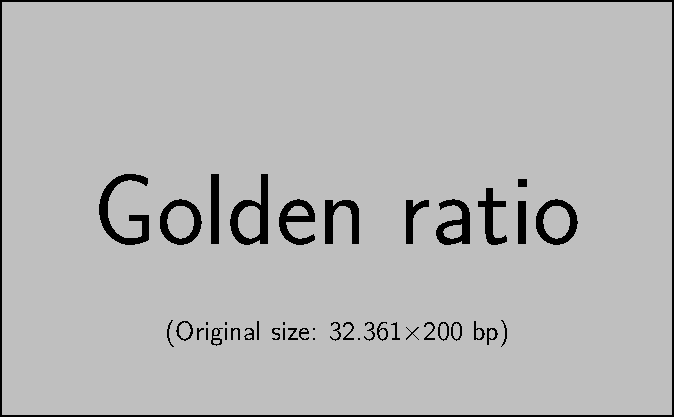
\includegraphics{placeholder_images/example-image-golden.pdf}
    \caption[Desirability index of various \glsfmtshort{rom}s]{A radar chart
        showing various the performance of various models compared against a
    desirability index (scale) sought after in all \glsfmtlong{rom}s}
    \label{fig:spiderdiagram}
\end{figure}


From \cref{fig:spiderdiagram}, it is  evident that all physics-based \glspl{rom}
presented thus far entail extensive  parametrisation efforts \fxnote{at the end,
count and  substitute the canonical  number of  parameters here} to  render them
suitable  for a  practical application.  The difficulties  associated with  such
parametrisation, coupled  with inherent uncertainties in  the obtained parameter
values  act as  a strong  deterrent to  stakeholders outside  academia to  adopt
\glspl{pbm} for  online implementation in  a \gls{bms}. This motivates  the need
for even further simplified \glspl{pbm}. One such modelling candidate is briefly
introduced next and is analysed in detail in \cref{ch:spmanalysis}.


Haran~\etal{}~\cite{Haran1998}  proposed a  highly simplified  representation of
porous  electrodes for  the metal  hydride cell  chemistry. In  this work,  each
porous electrode  was represented as  a single spherical particle.  This concept
was adopted for lithium ion batteries  by Ning and Popov~\cite{Ning2004} and has
since  become quite  popular.  Models employing  this  lumped representation  of
electrodes are referred to as  \glsfmtlong{spm}s (\gls{spm}s). These models have
three  advantages.  Since they  involve  only  a  subset  of parameters  of  the
original \gls{dfn}  model, most of them  being geometric quantities that  can be
directly measured without extensive  chemical or electrical testing, \glspl{spm}
are  easier to  parametrise than  other physics-based  \glspl{rom}. Furthermore,
they  are computationally  cheap, especially  when coupled  with the  polynomial
approximation  for solving  the  solid diffusion  equation  for each  electrode.
Finally, all model parameters in  the \gls{spm} retain their physical character,
aiding in  a direct and  intuitive understanding  of physical parameters  on the
cell's operation.

This concludes  the author's review of  literature of the various  reduced order
modelling  strategies. Based  on the  wealth  of information  gleaned from  this
study,  it was  possible to  make  an informed  choice to  pursue the  \gls{spm}
approach  for further  research.  In particular,  it came  to  light that  there
has  been  no systematic  analysis  of  the  state  of the  art  \gls{spm}-based
approach with  a view  to quantify their  performance boundaries.  This author's
contributions to  the time-domain  implementation-focus reduced  order modelling
field include
\begin{itemize}[noitemsep,topsep=0pt, before={\vspace*{-0.25\baselineskip}}]
    \item a thorough analysis of the existing \gls{spm} variants ranging from the rudimentary to the sophisticated
    \item enumeration of issues plaguing each \gls{spm} variant, including current state of the art
    \item study of further literature on the current tactics to overcome the current challenges along with their associated drawbacks
    \item conducting a  wide range of hypotheses-driven trials in an attempt to enhance  the basic \gls{spm} (some of which did not yield the desired
        improvements), and
    \item arriving at  a  feasible  approach  capable  of  moulding  the
        \gls{spm}  framework into  a  readily implementable  solution in
        electric vehicle applications
\end{itemize}
This research was  performed through an iterative cycle of  analysis, design and
simulation-based verification  and shall be  elucidated in a  discourse spanning
two chapters \viz~\cref{ch:spmanalysis} and \cref{ch:newelectrolytemodel}.



   % Literature Review
\setcounter{chapter}{2}
% -*- root: ../../main.tex -*-
%!TEX root = ../../main.tex

\graphicspath{{chapters/layer_opt/figures/}}
% ----------------------- contents from here ------------------------

\chapter{Model-based Design Of Pouch Cells}\label{ch:modelbaseddesign}
\vspace*{-1em}
\startcontents[chapters]
\printcontents[chapters]{}{1}{\setcounter{tocdepth}{1}}

\bigskip

\begin{figure}[!bp]
    \begin{minipage}[t]{\textwidth}
        \centering
        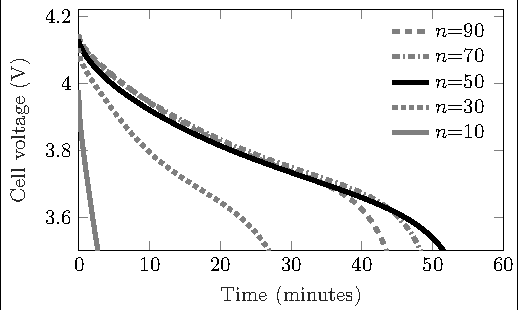
\includegraphics[trim=4 4 2 4,clip]{fig_CC_discharge_curves.pdf}
        \caption
        [%
        Voltage  curves   for  a   \SI{60}{\ampere}  galvanostatic   discharge  from
        \SI{100}{\percent} \glsfmtshort{soc}  until cut-off voltage for  a few layer
        choices, in a pouch cell of fixed exterior height.
        ]%
        {%
            Terminal  voltage curves  of a  Li-ion  cell (with  parameters given  in
            \cref{tbl:CellParams}) under a  \SI{60}{\ampere} galvanostatic discharge
            beginning from \SI{100}{\percent}  \glsfmtshort{soc} until lower cut-off
            voltage for a  few layer choices~$n$, in a pouch  cell of fixed exterior
            height. The maximum usable energy is achieved for an intermediate choice
            of $n$  that corresponds to  neither the highest nominal  capacity layer
            configuration  ($n$=\num{10}) nor  the  highest  electrode surface  area
            configuration ($n$=\num{90})\footnotemark.
        }%
        \label{fig:fig_CC_discharge_curves}
        \mpfootnotes[1]
        \footnote{This figure was created by Ian Campbell who asserts copyright,
            with  intellectual  contributions  from  and   the  right  to  use  asserted  by
        Krishnakumar Gopalakrishnan.}
    \end{minipage}
\end{figure}

% -*- root: ../../main.tex -*-
%!TEX root = ../../main.tex

\begin{table}[!htbp]
    \caption
    [%
    Theoretical  capacity \&  usable energy  of a  Li-ion cell  for a  few layer
    choices under a \SI{60}{\ampere} galvanostatic discharge
    ]
    {%
        Theoretical capacity and usable energy of a Li-ion cell (with parameters
        given in \cref{tbl:lcoSimParamslayeropt}) for  a few layer choices under
        a \SI{60}{\ampere} galvanostatic discharge.
    }%
    \label{tbl:CC_discharge_curves_table}
    \centering
    \begin{tabular}{@{} S[table-format=2.0] S[table-format=1.2] S[table-format=2.2]  S[table-format=3.2] S[table-format=2.2] @{}}
        \toprule
        \multicolumn{1}{@{} l}{$n$} &  \multicolumn{1}{c}{\footnotesize C-rate} & \multicolumn{1}{c}{\footnotesize \makecell{Theoretical \\ Capacity  (\si{Ah})}} & \multicolumn{1}{c}{\footnotesize \makecell{Usable \\ Energy \si{(Wh)}}} & \multicolumn{1}{c @{}}{\footnotesize \makecell{Remaining \\ SOC  (\si{\percent})}} \\
        \midrule
        90 & 1.24 & 48.25 & 166.46 & 9.84  \\
        70 & 1.11 & 53.99 & 184.80 & 10.26 \\
        50 & 1.00 & 59.73 & 195.47 & 13.51 \\
        30 & 0.92 & 65.47 & 101.20 & 58.95 \\
        10 & 0.84 & 71.21 & 10.15  & 96.22 \\
        \bottomrule
    \end{tabular}
\end{table}


\begin{figure}[!bp]
    \begin{minipage}[t]{\textwidth}
        \centering
        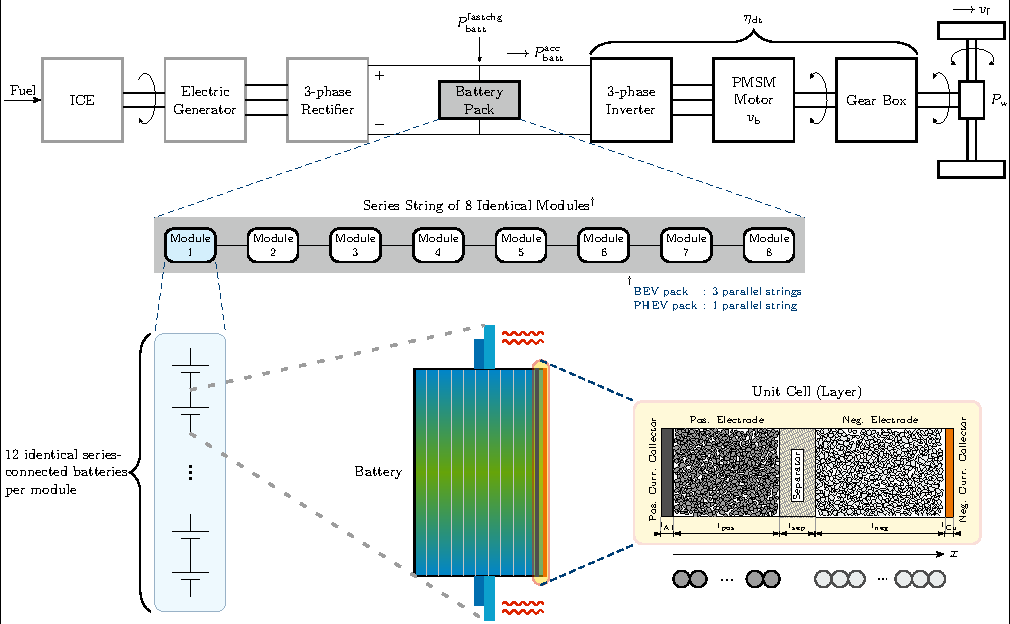
\includegraphics[width=\textwidth]{hierarchical_powertrain_to_cell_layer.pdf}
        \caption
        [%
        Vehicle-to-cell hierarchical  overview of  an electrified powertrain architecture.
        ]%
        {%
            Schematic  depicting   the  vehicle-to-cell  hierarchical   overview  of
            a  typical   electrified  powertrain   architecture.  This   represents  the
            system-level context within which  the proposed layer optimisation framework
            has been developed. Two \glsfmtshort{xeV} powertrains ---
            \begin{enumerate*}[label=\itshape\alph*\upshape)]
                \item  a \gls{bev}, and
                \item  a series \gls{phev}
            \end{enumerate*}
            are  chosen as  examples  to demonstrate  how  the methodology  facilitates
            common module designs for such battery packs\footnotemark.
        }%
        \label{fig:fig_PowertrainSchematic}
        \mpfootnotes[1]
        \footnote{This  figure was  created by  Krishnakumar Gopalakrishnan  who
            asserts copyright, with intellectual contributions from and the right to
        use asserted by Ian Campbell.}
    \end{minipage}
\end{figure}

\afterpage{%
    \clearpage
    \thispagestyle{plain}
    \begin{figure}[p]
        \begin{minipage}[t]{\textwidth}
            \centering
            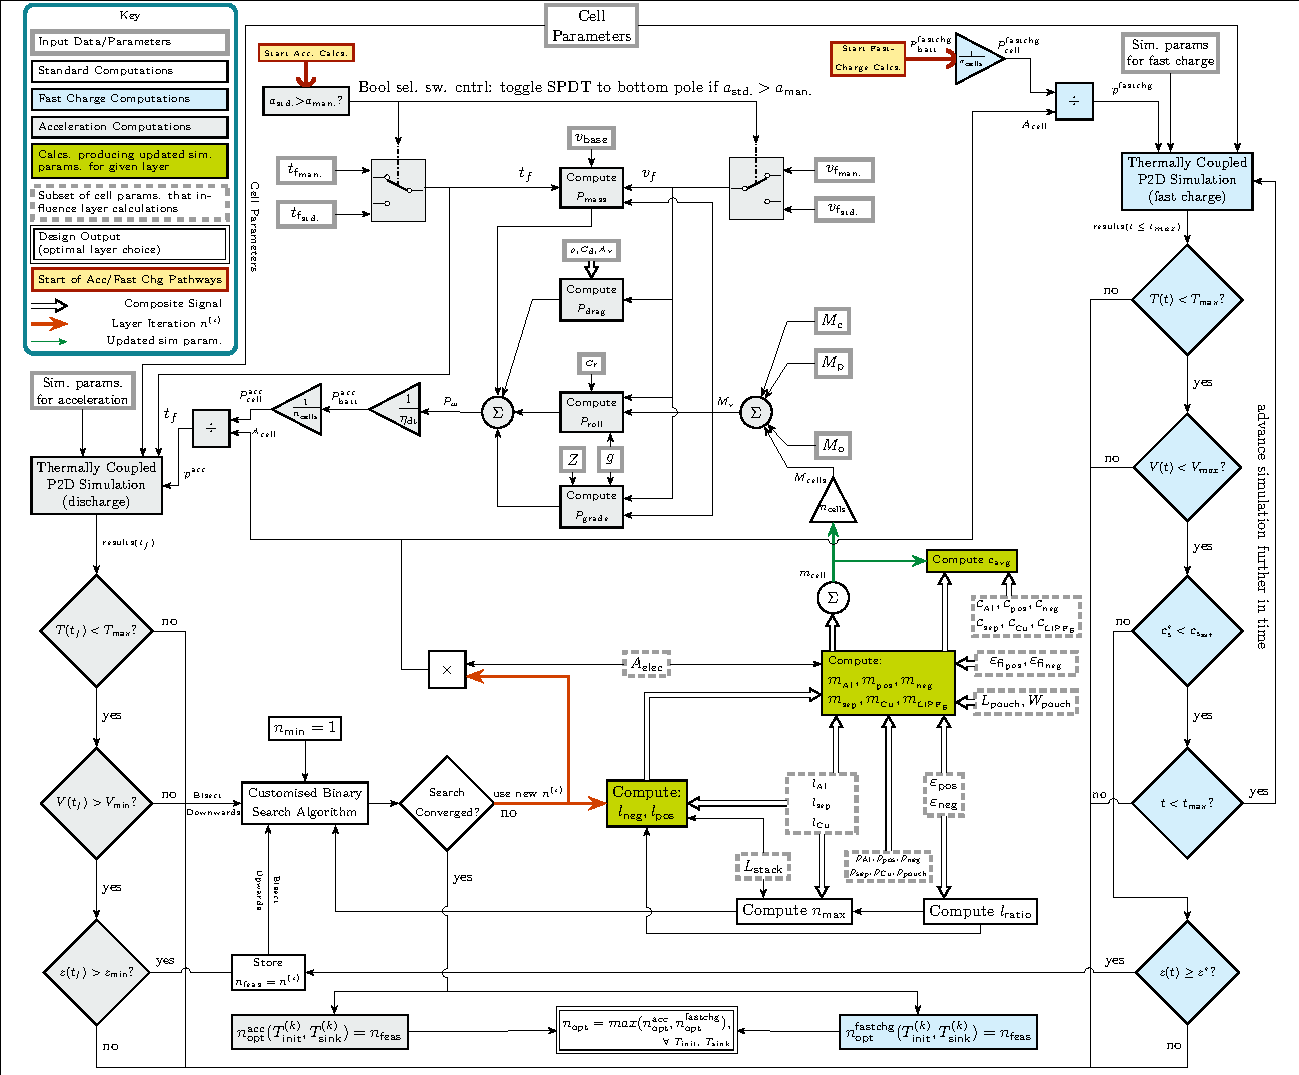
\includegraphics[angle=90,width=\textwidth]{fig_master_flow_diagramPDF}
            \caption
            [%
            Flow diagram depicting an overview  of the proposed layer optimisation methodology
            for Li-ion pouch cells.
            ]%
            {%
                Flow diagram depicting an overview  of the proposed layer optimisation methodology
                for Li-ion pouch cells\footnotemark.
            }%
            \label{fig:fig_strategy_schematic}
            \mpfootnotes[1]
            \vspace*{1.125cm}
            \footnote{This  figure was  created by  Krishnakumar Gopalakrishnan  who asserts copyright, with intellectual contributions from and the right to use asserted by Ian Campbell.}
        \end{minipage}
    \end{figure}
}%


%Honour  code pledge:  This  chapter  plan was  written  without  looking at  the
%manuscript even  once. Only the actual  code commits of LIONSIMBA,  BOLD toolbox
%and the data from shared Box folder was used in writing this up.

%The literature review for this chapter shall be split over two parts - the first
%part shall be in a separate literature review chapter. The other part will be in
%this chapter,  but peppered in  multiple areas/sections. To clarify,  the second
%part  shall deal  with the  literature  pertinent to  the section  whence a  new
%concept is introduced.

%\section{Literature  Review Chapter}
%This shall  present an  inverted pyramidal  overview on  the topic  of model-led
%design of lithium ion  cells. The review exercise shall aims  to bring to light,
%the glaring  contrast between  the cornucopia  of literature  discussing various
%aspects  of drivetrain  design versus  the relative  paucity of  published works
%dealing with cell-level design optimisation for electrified transport.

%The literature review shall be broken up into sections as follows.

%\section{Drivetrain design Optimisation}

%Two to three paragraphs discussing  the published works (actual journal articles
%in  SAE etc.\  authored by  automotive companies)  dealing with  all aspects  of
%drivetrain  design. This  includes two-three  sentences describing  special care
%touching topics of choice of gearing ratios, motor speed-torque-efficiency curve
%discussion, choice  of rare-earth materials  for motors, choice of  motors, body
%chassis for minimizing drag.

%A detailed publication on  the ins and outs of the  Prius drivetrain analysed by
%OakRidge  National  Labs  will  be  reviewed. Its  figures  shall  be  used  for
%highlighting motor-speed torque curves,  choice of power electronics, schematics
%of bi-directional converters etc, and any (there are many) relevant figures that
%may be used.

%A  remark  or  two  about  typical  efficiencies  of  components.  Basically  my
%drivetrain course  and the Emadi  textbook cited and  relied upon as  source for
%material

%My  own  course  on  drivetrain  design shall  be  cited  and  the  optimisation
%exercise/homework be quoted.

%This author  recognizes that this  is a huge  topic of interest  in conventional
%mechanical and  automotive engineering, the  idea is  not to do  a comprehensive
%literature review on  this well-established field, but nevertheless use  it as a
%crutch  to  bring  out  the  stark  contrast  in  the  published  literature  on
%battery-specific  design. It  will become  clear that  manufacturers and  system
%integrators  rely  mainly  on  equivalent  circuit or  even  bucket  models  for
%drivetrain design optimisation. They cannot be entirely blamed, since this is an
%inherently  multi  scale problem,  how  design  optimisation  can be  done  with
%fine-grained physics-based pack models is still a research question.

%In particular, at the  end of this section, it should drive  home the point that
%design  optimization  is  being  performed  in  every  field  other  than  at  a
%battery/cell level. This  author hypothesises the cause to be  attributed to the
%relative  infancy  of  the  subject  as well  as  possible  secrecy  among  cell
%manufacturers/battery systems  engineers. A  need to study  this field  shall be
%pointed out.

%\section{Battery Design Optimisation}

%Group  of cells  arranged into  modules  and then  connected in  series/parallel
%strings to form battery pack. The state  of the art in battery pack design shall
%be reviewed  in a  few paragraphs. Only  the relevant works  will be  cited. Our
%focus is on optimisation of pack design.

%The  literature  covering   pack  design  optimisation  shall   be  covered.  In
%particular,  about adherence  to  standard  to design  modules  below  50 V  for
%safe  handling by  technicians  can be  viewed  as a  constraint  on the  design
%optimisation.  Very historic  views  shall  only be  mentioned  and not  covered
%in-depth.

%\subsection{Thermal Design}

%System level pack thermal design shall be acknowledged as a complex topic beyond
%the scope of this work. How inner cells  in the pack are typically a few degrees
%hotter than the outermost cells. Finite-Volume based CFD analysis is the norm in
%this field  and is  usually done  by a dedicated  thermal engineering  team. The
%interested reader shall be referred to the relevant literature.

%However,  one important  takeaway that  will  later influence  and dictate  this
%author's study  with respect  to pack  thermal design is  the choice  of cooling
%mechanism. In the view of the  experimental results revealed by Ian Hunt's paper
%on tab  cooling, particularly, the uniform  thermal gradient across layers  in a
%pouch cell, particularly helps to represent an individual cell's electrochemical
%properties  (composed of  many layers)  through  a representative  study on  one
%layer  using the  P2D model.  For a  standard surface-cooled  pack design,  this
%implies  that for  cell modelling,  two dimensions  must be  considered for  the
%electrochemical and coupled thermal phenomena.

%\subsection{Pack Layout}
%Common system  bus voltages  shall be  listed, which will  entail the  number of
%series connected cells  in each string. Choice of number  of parallel strings to
%determine the  energy content of  the pack, and hence  the driving range  of the
%vehicle. With  this considerations  in place, the  literature on  arrangement of
%packs shall be presented.

%There   are  a   couple  of   literature  dealing   with  optimisation   of  the
%series-parallel  matrix arrangement.  Some  real-world constraints  and how  the
%literature handled them shall be discussed.

%\section{Cell Design}

%Cell Design (even within the narrower  lithium ion chemistries) is a complex and
%hugely active area of  research. The wealth of literature is  much more than one
%could possibly review  in a thesis, and  spans topics in synthesis  of new anode
%and cathodes (cite some recent research here), new electrolyte salts and organic
%solvents  that  remain  stable  and  inflammable  beyond  5V,  intelligent/smart
%separators that shut down their pores in  the event of thermal runaway etc. Very
%brief listing only of  the most important papers in the last  2 years only, just
%for roundedness.  This broad  cell design  overview concludes  with a  view that
%while  the future  is  exciting  and certainly  deserves  investment,  a lot  of
%breakthroughs are still in the pipeline and not ready for primetime.


%Squeezing out  every last ounce of  juice left in batteries,  while not damaging
%them  is of  prime interest  to manufacturers  today to  quell range  anxiety of
%customers.  Similarly, the  charging time  is a  bottleneck in  real-life usage.
%Therefore, to tackle  an immediate demand, we focus on  the optimisation of cell
%designs  based  on  existing  materials  for which  supply  chains  are  already
%well-established.

%\subsection{Practical Approaches to Cell Design Optimisation}

%In the view of this thesis author, cell design optimisation can be carried out through
%\begin{itemize}
%    \item Empirical approaches
%    \item Systematic Experimental approaches
%    \item Model-led approach
%    \item and/or an iterative combination of the three above
%\end{itemize}

%Give  one  example each  of  empirical  design  and  experimental design  and  a
%combination of them. Cite through review of relevant literature on how they have
%successfully taken off.

%Explain  why model-led  design optimisation  is still  lagging behind  empirical
%optimisation.  Physics-based  models  have  too many  parameters.  Criticism  on
%parameterisation.  Each cell  manufacturer  has  a custom  cell  design that  is
%shrouded  in secrecy.  Examples  include in-house  ingredients  for binders  and
%fillers and enhance the electronic  conductivities of the active material matrix
%while ensuring that the electrodes remain  stable. Such art are never published.
%Even system  integrated tasked with optimisation  of the drivetrain do  not have
%access  to  the  individual  electrode-level/electrolyte-level  enhancements.  A
%teardown of the cell can at most reveal the geometric parameters of the cell and
%may offer a  clue to some physical properties of  the material. Parameterisation
%involve specalised  lab equipment  that is often  available only  to large-scale
%test  facilities (SEM,  porosimeters)  in specialised  academic  labs. There  is
%also  a culture  of lack  of  information sharing  or NDAs  signed that  prevent
%publishing of  such information  . However, without  definitive parameterisation
%and co-operation  between cell  manufacturers and system  integrators, model-led
%cell  design  has  suffered,  although  it   is  of  need  of  the  hour  (until
%more  material-level  fundamental  breakthroughs  are  available).  Explain  how
%this  interdisciplinary  field  involving   numerical  expertise  and  intricate
%electrochemical knowledge can  lead to better design of  batteries that benefits
%all.

%Dwell  on  the  advantages  of   a  model-led  design  optimisation  like  rapid
%prototyping  and minimising  time  to first  production  yield. Offer  parallels
%through  published  literature  on  the  areas  where  this  has  been  deployed
%successfully.

%Now,  discuss  literature, wherein  despite  limited  parameters are  available,
%academia and industry have worked hand-in-hand to optimise electrode thicknesses
%and  porosities. There  are  two-three  strong literature  in  my Mendeley  (Ian
%did  not  yet  give  me  access  to our  shared  Mendeley)  that  discuss  these
%optimisation studies made, however, from an experimental point of view. There is
%nothing missing  from a modelling point  of view. Modelling results  followed by
%experimental confirmation  is the  method of  science that  can be  employed for
%robust progress in the field.

%Conclude with a view that there has  been an obvious skip (a jump) in literature
%that  is  glaring  and  in  plain  sight.  From  an  electrified  transportation
%perspective,  there has  been  plenty of  system-level  analysis discussing  all
%aspects  of system-level  pack design  (electrochemical, thermal  and placement)
%mostly  done by  industry folks.  At  the other  end  of the  spectrum, we  have
%academicians and  government research  labs toiling  away at  microscopic scale,
%synthesising materials, which  may be years before being available  at scale for
%mass-adoption. The  closest thing  we have now  is experimental  optimisation of
%electrode thicknesses and  porosities that is both  intensive and time-consuming
%and not attractive  as a drop-in optimisation solution to  industry. The obvious
%jump in scale is from the system level down to electrode-level. Pouch cells form
%the majority of automotive-grade cell type (refer intro chapter). There is a key
%design choice that can be optimised here \viz{} the number of layers. Literature
%is  missing  this in  entirety  with  not  a  single published  work  discussing
%optimising  the  number  of  layers,  at-least  from  a  model-led  perspective.
%The  author's work  therefore  discusses  this critical  aspect  of cell  design
%optimisation in chapter so and so.


%The above paragraphs were in a  dedicated chapter and the following content goes
%into the chapter. This paragraph is written here only for the chapter plan.

%\section{Chapter Introduction}

%A statement  of thanks and  acknowledgement upfront  that this work  was jointly
%undertaken with  Ian Campbell. Relevant  sections where Ian's help  was obtained
%are attributed in-line,  with an attribution statement  identifying the specific
%nature of his support.

%A brief 1-2 sentences throwback to the literature review, referring what we will
%say in this chapter.  Explain the goal of this chapter, to  arrive at the number
%of layers to meet  a given energy and power demand. The outcome  is that a ready
%to  use tool  is made  available to  validate empirical  layer choices.  Special
%emphasis is  placed on the  \emph{methodology} since the  results per se  do not
%stand alone outside of the modelling regimen (universe we created). However, the
%value  is on  the  methodology and  its  implementation in  a  toolbox which  is
%immediately  available  for  download  and  use by  industry  to  confirm  their
%empirical layer designs.


%%In the absence of access to cell manufacturing facilities to confirm and test the layer
%% Immediate adoption in industry.

%\section{Energy to Power Trade-off}
%Impart knowledge on  energy cell versus power  cell with the help  of a diagram.
%Explain the effect of useable energy and power for a given cell with the help of
%a figure and table. How layers place  a role in controlling this trade-off shall
%be discussed in the subsequent sections.

%\section{Augmentation of P2D parameters}

%Shed more light on the p2d model. Explain  how they do not model a cell of given
%capacity, but instead  work on a normalised basis driven  by the applied current
%densities rather than  the external current. The parameter that  layers within a
%cell  change  is  the  overall electrochemically  active  cross-sectional  area.
%Criticise  how  published literature  curiously  omit  this important  geometric
%parameter, however  they may  be forgiven in  the scope of  their work  since it
%needs only normalised  dynamics. This parameter comes into  light when modelling
%anything involving geometries as in this project. This is the product of surface
%area per face and the number of  layers. To determine the surface area per face,
%the author has derived a new  methodology/process involving a sequence of steps,
%based on assumptions and literature search.  The process involves selection of a
%real-world cell, and ultimately mapping it to the surface area per unit face. To
%the best  knowledge of  the author,  this mapping  from a  physical cell  to the
%Newman model is  unique and is claimed  as the author's own  contribution to the
%art.

%Describe briefly  the process  of mapping  a real-world  cell onto  the standard
%\gls{p2d} model.

%Note: Krishna wrote the Northrop to EV mapping code and explained the concept to
%the mapping to Ian. Ian's help on the matter is identified where relevant.

%\subsection{Modelling Platform and Preconditioning}

%Couple of  statements about why LIONSIMBA  was chosen as the  modelling platform
%for implementing the  P2D dynamics. The cell parameters used  are shown in table
%xx. This cell is henceforth known as the LIONSIMBA cell or Northrop cell.

%Discuss  the missing  elements in  LIONSIMBA only  with respect  to the  present
%problem  at hand,  \viz{the  stoichiometries}.  Thanks to  Ian  for running  the
%time-intensive and  memory-intensive simulation  process on his  workstation and
%offering comments on datalogging.

%\subsubsection*{Stoichiometry Augmentation}
%Discuss the problem first. How LIONSIMBA  started always at 85.51 percentage and
%needed to  do a  discharge down  to zero  percent before  having the  ability to
%charge. For this  project, stoichiometries are vital  for capacity determination
%and  the 1C  current density.  Explain  how stoichiometries  were refined  until
%cut-off for  infinitesimal bleeding  discharge current achieved.  Noted relevant
%values. Explanation with detailed figure on how stoichiometries were found to be
%missing. Explain refinement  of how approximate capacities  reported by Northrop
%and Subramanian  were refined precisely.  Explanation of remnant  capacities and
%stoichiometries computation.  Explanation of  1C current density.  Note: Krishna
%wrote the parameters  init capacity computation code. Thanks to  Ian for running
%the simulation

%\subsection{Selection of a Suitable Reference Capacity Cell}

%Explanation of how  the Bolt EV cell  was selected (state of the  art in driving
%range) In particular, explain how the critical computation of 60 Ah capacity was
%done. Furthermore, convincingly explain how a  pouch cell thickness of 10 mm was
%used with all the background references.

%Note: Krishna did this thorough literature review, whose proof is available with
%timestamp in Box. Krishna would like to  thank Ian for his time in brainstorming
%the exact BEV to use. This phase lasted a couple of weeks. For the PHEV, Krishna
%and  Ian jointly  did the  PHEV literature  search, and  since Krishna  does not
%intend to  go in depth  for PHEV results,  Ian may choose  to use it  and simply
%acknowledge Krishna.

%\subsection{Layer Assembly within Pouch Cells}
%With  the  help   of  Northrop's  layer  assembly  figure,   explain  the  layer
%configuration/arrangement within a pouch cell.  The next task is then identified
%as computing the number of layers within the pouch cell.

%\subsubsection*{Number of Layers of LIONSIMBA aka Northrop cell}
%Krishna came up with  the idea of using integer optimisation  for this task. The
%software MIDACO  was also selected by  Krishna and explained to  Ian. The MIDACO
%result of the number of layers within the standard cell was now available.

%\subsubsection*{Computation of Surface Area per face, \protect{$A_\text{cell}$}}
%Show  the simple  algebraic  computation of  overall surface  area  $A$ and  the
%per-face area  $A_\text{cell}$. Explain  how the  area per face  shall be  a key
%quantity in the layer optimisation framework discussed later on.

%Layerphoto showing face areas and anode/cathode verhand etc will be shown here

%This concludes the augmented set of parameters  added by the author to the basic
%parameter set  of the  DFN model.  The added numerical  value of  parameters are
%summaried in table xx. Lots The  layer optimisation framework and assumptions is
%described next. % table: pouch length, width, tab area, stack thickness etc.

%\section{Layer Optimisation Framework}

%Basically the  pack configuration and the  universe in which we  worked shall be
%discussed here with  the help of the  hierarchical powertrain-to-cell schematic.
%This will set the context of  the problem being tackled. Important concepts that
%enable the creation of the universe in  which we define the problem to be solved
%in discussed and the assumptions involved shall be explained.

%The layer optimisation  framework hinges upon the concept  of capacity balancing
%between electrodes.  Explain this  nicely with references  and citations  on why
%this is important. Helps us make us  of the most of the active material invested
%into the cell.


%\subsection{Capacity Balancing}
%Formula for capacity  balance. Show how the length of  the negative electrode is
%slightly larger than the positive electrode,  but compensated for by the reduced
%volume fraction.  Cite other  parameter sets  where this  is observed.  They are
%nearly equal, but made to be 1.10

%Note:  This  1.1 ratio  was  fixed  by Krishna.  I  can  explain in  person  how
%this happened  (reason: numerical  convergence). The  thickness of  the positive
%electrode was adjusted accordingly. If Ian is asked this question and details of
%its origin, Krishna is sure he cannot explain it.

%\subsection{Electrode Thicknesses per layer}
%Talk briefly about separator and how its thickness remains constant.

%With this,  show the  mathematical derivation  of the  expression for  number of
%layers Explain  the significance of the  outermost layer and how  it affects the
%formula used Explain how the stack  is formed. Report its numerical value. Pouch
%thickness and  its role  along with  suitable reference.  Show briefly  a clever
%computer code snippet that encapsulates both cases of odd and even.

%At  this stage,  can explain  clearly the  relationship between  the theoretical
%capacity  and  number of  layers.  Use  a graph  or  a  table to  highlight  the
%idea.  Useable  capacity shall  be  lower  than  total  capacity due  to  cutoff
%considerations. Explanation.

%Note:  Again,  Krishna   explained  the  layer  calculation   formulae  to  Ian.
%Especially, the derivation of the  combined electrode thickness concept, and the
%usage of  the ratio  to obtain  one from  the other.  Ian had  to write  it down
%multiple times  drawing the layers and  verify that my computation  was correct.
%Krishna  explained  how  the  cases  environment can  be  used  for  theoretical
%description while the computer code for both  the cases uses ceil and floor. Ian
%naively used  the mathematical symbol for  ceil, until Krishna explained  to him
%about the  cases environment. Krishna  also typed up these  equations (basically
%any equation that required a derivation) in the paper manuscript.

%\subsection{Derivation of analytical \protect{$n_\text{max}$}}

%The  search space  spans  a  finite number  of  layers.  An initial  alternative
%considered was MIDACO. The detailed equations  and how they are derived go here.
%Discuss for both odd and even cases. However, closed form analytical expressions
%are now available. This  is so as to enable a binary search  as discussed in the
%next section.

%The optimisation formula and analytical solution shall also be discussed here.

%Note: Krishna is claiming the idea  generation and coding in entirety. The mixed
%integer optimisation to zero thickness was some fancy coding. The zero thickness
%idea was  also quite  fancy. Krishna  came up  with the  whole of  this section.
%Initiated the  idea of narrowing  down the search  window. Ian was  content with
%doing a for loop since it will also  work. The optimal layer in this case is the
%earliest choice of $n$ in the for  loop for which the termination conditions are
%correctly satisfied.  Krishna was always  in favour of an  optimisation approach
%from the beginning.

%\subsection{Customised Binary Search}

%A  bi-section  based algorithm.  Algorithm/binary  tree  based description  with
%figure/algo. Discuss the O(log n) speedup.

%Note: One fine evening, Krishna increased the computational speedup by two orders of magnitude. Proof in github and email. While Ian was always interested in a for-loop approach right from beginning, Krishna always suggested to use an optimisation approach.

%\subsection{Mass recomputation as a function of layers}
%Explanation with graph.

%\subsection{Specific-heat recomputation as a function of layers}
%Suitable explanation and plot.

%Note: Ian  congratulated Krishna for mass  and specifc heat computation.  In his
%words,  ``You were  clever coming  up with  a scheme  wherein mass  varies as  a
%number  of  layers''.  Packaged  this  up  as  a  function  and  all.  Refer  to
%computelumpedmassandCpavgforgivenlayerfcn. Can prove git  history for this file.
%Not  only mass  recomputations but  also mass  initial computation  was done  by
%Krishna

%\subsection{Thermal space permutation of layers.}
%Explanation of how the four corner temperatures are tried here. 5 lines of code snippet that packs a punch

%Note: Krishna read the acceleration specification description,educated Ian and implemented this.

%\begin{quotation}
%Ian: Krishna!. Whoa that small block of code does so much.
%\end{quotation}

%\section{Workflow for Optimal Layer Computation}

%This section  discusses the  actual methodology  or the  procedure in  which the
%aforementioned ideas are incorporated in  a process-like workflow. Introduce the
%full-page crazy flow  diagram here. Explain how the flow  diagram goes through a
%methodical  approach in  arriving at  the  optimal number  of layers.  Extensive
%forward  and  backward referencing  to  sections  discussing each  modular  idea
%encountered  in  the flow  path.  Discuss  how  the  applied current  and  power
%densities  change due  to  change  in overall  surface  area  while the  applied
%external current/power remains the same.

%% This will help us to apply current in units rather in current density.

%The salient cases to be covered are the following.

%\subsection{Case 1 --- Analysis of Drivecycle Powers}

%Although  from  Colorado  Boulder  lecture  notes,  Krishna  already  knew  that
%acceleration demands the highest power demand on the cell, it needs to be proven
%that drive cycles, which are the  basis for various fuel efficiency calculations
%do not represent this case. Ian did the comparative study of various drivecyles.
%Some  plots and  charts  showing various  power levels  were  generated by  him.
%Krishna does  not explicity  need to use  this section, and  is optional  to the
%story, other than the sake of well-roundedness and demonstrating thoroughness of
%the study.

%Explain that this case is not present in the flow diagram.

%However,  it  was  Krishna  who  generated the  drivecycle  speed  vs  time  and
%acceleration versus time results alone and  then informed Ian afterwards that it
%is now available in the repository. If Ian uses this section, an acknowledgement
%will be appropriate.


%\subsection{Case 2 --- Acceleration from standstill}

%Explanation and computations  based on standard vehicle  dynamics. Lecture notes
%and videos given to Ian by Krishna  from Univ of Colorado Boulder The sole value
%addition in this  case is the specification to adhere  to and its implementation
%through  a cases  study. Krishna  shall explain  this through  either-or if-then
%case, explanation along with a short code snippet which he implemented alone.

%Explain the  acceleration run in detail,  what it entails etc.  Walk through the
%flow diagram till acc layer results are discussed.

%Note: The acceleration specification for  electrified transport was unearthed by
%Krishna  (all the  interlibrary  loan  stuff and  educated  Ian  about it).  Two
%passengers and all that thing. Complete coding.

%\subsection{Case 3 --- Fast Charging}

%A brief  explanation of the whys  and the hows and  implications. Explanation of
%prevalent standards. Present table of standards etc etc

%One paragraph  review of control algorithms  and how this algorithm  was chosen.
%Brief  overview of  algorithm. The  idea  of introducing  saturation and  pulsed
%charging profile. Based  on patent at Auburn university.  Krishna did literature
%review.  Flag  introduced   in  code.  Code  snippet.enablecsnegsaturationlimit.
%% Sinusoidal excitation charging.

%Explanation of why power demand is important (based on charger power electronics).
%Finally, walk through of the fast charging section of the schematic.

%Note: Krishna  performed the litt  search of  this section entirely  (proof with
%timestamp available). However, Krishna is  tentatively not using a detailed litt
%review.  In kind  consideration of  Ian's  own overarching  thesis topic,  which
%Krishna understands to be something pertinent  to fast charging, Krishna can let
%Ian use the literature provided proper attribution  is in place. For the sake of
%completion, the  MIDACO based approaching  to fast charging showing  the pulsing
%power is also possible by Ian (just a suggestion).

%Note: The charger  power electronics limit is again my  contribution from an EEE
%background

%% \item Review of model-based fast charging control algorithms (how does this go into litt review)

%\section{Simulation Environment}
%Discuss parameters of  simulation environment. Discuss with the help  of a table
%for the  BEV case only. Ian  can take the PHEV  Number of BEV calls  designed to
%make up the series string.

%Krishna  also came  up with  the cell's  cutoff study  with respect  to the  the
%system's  bus bar  voltage, and  will  be cited  here with  examples and  strong
%backing. There  are a few  preconditioning steps needed  to amend the  P2D model
%before  numerical implementation  of the  flow  diagram is  possible. 1.  Fixing
%aspects of  the code  in LIONSIMBA v1.023  used as the  baseline by  this thesis
%author. 2.  Addition of the capability  to apply power input  instead of current
%input as is common in traditional p2d simulations.

%Note:  All crucial  parameters  were  sourced by  Krishna  through a  literature
%review. Especially, the  vehicular parameters like classis  mass, coefficient of
%drag, base speed. Krishna also had to educate Ian about base speed. If an on the
%spot quiz is conducted  at a conceptual level, this truth  can easily be deduced
%by the judging authority. Krishna claims the literature review of this topic and
%is happy to let Ian use this with proper attribution.

%\subsection{Preconditioning of Computer Code}

%Briefly allude to the stoichiometries that was introduced into the computer code
%through capacity characterisation  simulation.Now possible to start  at any SoC.
%The other salient  amendments and enhancements to the software  toolbox is shown
%below. Released as 2.0 and link to LIONSIMBA github repo (not BOLD toolbox repo)

%\subsubsection{Re-parameterisation}

%Discuss  the  extensive Reparameterisation  undertaken  by  Krishna by  studying
%relevant literature.  Discuss the  changed parameters  with respect  to Northrop
%cell and why. Maybe show a table. This is quite substantial.

%Conductivity/diffusivity changes.  Show how the isothermal  and thermal variants
%in existing Northrop cell were bogus with plots.

%Performed  comprehensive   literature  review   to  replace   the  dubious/bogus
%parameters of the electrode and electrolyte specific heat capacities email proof
%PS:  Every thermal/material  property of  the Al/Cu  current collectors  is very
%clear and have been traced out, hand-calculated and validated.

%\subsubsection{Deterministic initialisation  of algebraic variables}

%Replaced silly fsolve. Numerical explanation here.

%\subsubsection{Linear interpolation for field variables}

%Explain how  linear interpolation was performed  for phis and phie  at the edges
%of  control volumes  in  electrode  and separator.  Draw  a  schematic for  this
%explanation.

%\subsubsection*{Convergence Analysis of Computation Mesh}
%Report  only   if  Krishna  has   sufficient  time  left.   Explain  simplifying
%assumptions.  Refer to  the  table etc  Show  plot of  how  terminal voltage  is
%converging for chosen mesh as a function of number of nodes. Another plot of how
%simulation end time converges as a function of number of nodes. Lots of analysis
%by changing the number of nodes within  each mesh to justify the validity of the
%results. Prove that mesh independence is reached.

%\subsection{Hybrid FV--Spectral Scheme}

%Completely numerical section.  Highly mathemetical. Explain how  the rational to
%decimal  truncation of  the unbalanced  twelfth order  finite difference  scheme
%messes  up numerical  conditioning.  Show matrices  and  discuss the  drawbacks.
%Fornberg matrix did not help. So, spectral scheme was needed.

%Background  study,   explanation,  analysis,  literature  review   and  equation
%derivation  of spectral  scheme Complete  contribution of  solid-phase diffusion
%with spectral methods. Reading textbook, understanding concept, investigation of
%applicability,  hunting relevant  literature,  text-writing, hand-derivation  of
%equations. This complete section was done by Krishna.

%\subsection{Lumped Thermal Model}

%Basic discussion of lumped thermal model  and justify through citations why here
%it  might  be  sufficient  for  this  application.  Not  originally  present  in
%LIONSIMBA. Present  the thermal model here  equations here. Discuss what  cp avg
%means and how it is computed as a here function of number of layers. Explanation
%of how tab cooling helps here.

%Note: Cp  avg was calculated and  coded by Krishna,  as a function of  number of
%layers. I shall leave the detailed thermal model to Ian, especially since a biot
%analysis was performed by him. Anyway,  suddenly discussing the thermal model at
%depth does not fit the story of my  thesis. My hint to Ian would be to emphasise
%the thermal model  at depth, since anyway  he seems to be confident  in the biot
%analysis. Specifically  the value of  heat transfer coefficient  was empirically
%chosen  by Ian  through simulations.  So,  I will  let him  explain that  stuff.
%However, tab area idea computation using  twice the Bolt's tab area was proposed
%by Krishna,  but overall this thermal  stuff, Krishna is willing  to bequeath to
%Ian  since  the  whole thing  doesn't  fit  the  story  of Krishna's  work.  The
%polarisation heat  concept was initially described  by Greg, but anyway  let Ian
%explain it, no problem.  Ian may wish to discuss entropic  heat generation and a
%lot of  other things we investigated  together, but I  am not going to  dwell on
%them in the thesis.


%\subsection{Power Input Boundary Conditions}

%Discuss why power input is needed for layer optimisation. Explain how it is done
%currently in state of the art case.

%Krishna educated Ian about Pletts existing  work. Accompanied Ian to the library
%and told him to check out that book which I had ordered.

%Krishna  claims a  very important  thing here.  A critical  argument on  how the
%present schemes do not fit into the layer opt methodology.

%Detailed mathematical derivation. Both Ian  and Krishna acknowledge each other's
%help in shared derivation and also acknowledge Davide appropriately.

%Note: Ian might  wish to report the two intermediate  steps before this solution
%was obtained. The  2nd of the 3  approaches was matching current  and voltage at
%discrete intervals through  numerical integration. This was  our third approach.
%The first approach was too simplistic. So, Ian might wish to skip it.



%\section{Layer Optimisation Results}

%Show the table  only with the extra parameters not  present in isothermal model.
%In particular,  I can  remember the  thermal parameters  of the  two electrodes,
%separator, pouch, current collectors and electrolyte.

%Present the results in a horribly bland  table format steering well clear of the
%heatmap. Krishna's view is that the results do not stand alone by themselves and
%if you plonk  a layer choice from  the heatmap/table into your  cell, things are
%not expected  to work as is.  The numbers herein are  the result of quite  a few
%assumptions and hold validity only within the universe in which it was created.

%However, the framework itself is transferable and is the most valuable component
%of the  work. A user  reading this thesis can  easily substitute their  own cell
%parameters and system-level considerations into the code and obtain results from
%it accordingly.  This was the  working premise of the  paper as well,  until Ian
%decided to write up a bloated explanatory section.

%Plots of acceleration and fast charging for successful layer count.

%For PHEV, although common module design will be alluded to, it will not be dwelled on or explained or analysed in depth.


%Note: In Ian's thesis,  Krishna seeks attribution for the idea  to use a heatmap
%since it  arose out of  Krishna's heavy  criticism, bordering on  the offensive,
%about  continuously  complaining that  our  group's  plots/charts/graphs do  not
%exhibit any ``interesting'' twists and  turns and fancy illustrations. Apologies
%for this. Anyway, the heatmap idea was  my suggestion. However, I shall not take
%an inch of credit for the implementation as it was entirely Ian's work in coming
%up with fancy schemes.

%Note:  Having  obtained  BEV results,  Krishna  also  set  up  the full  set  of
%assumptions  for  the  PHEV  simulations too  before  leaving  actual  numerical
%simulations  to Ian  (and on  vacation  to India  followed by  Konstanz). So  an
%acknowledgement is  required if Ian  choses to  list these assumptions.  Ian can
%discuss monotonicity issues in PHEV simulation that he found out about.

%\section{Appendix}
%Intend to provide a call-graph in the appendix


       % Layer Optimisation
\setcounter{chapter}{3}
% -*- root: ../main.tex -*-
%!TEX root = ../main.tex
% this file is called up by main.tex
% content in this file will be fed into the main document
% vim:textwidth=80 fo=cqt

\graphicspath{{chapters/dra/figures/}}
% ----------------------- contents from here ------------------------

\chapter{Computational Analysis and Numerical Reformulation of the \glsfmtshort{dra}}\label{ch:improveddra}
% \chapter{Analysis of the \glsfmtlong{dra} and Performance Boost through Numerical Reformulation}\label{ch:improveddra}
% \chapter{Computational Bottleneck Analysis of the \glsfmtshort{dra} and its Mitigation through Numerical Reformulations}\label{ch:improveddra}
\vspace*{-1em}
\startcontents[chapters]
\printcontents[chapters]{}{1}{\setcounter{tocdepth}{1}}

% \bigskip

\capolettera{T}{his} chapter presents  an analysis and critical  evaluation of a
computational bottleneck present in  a popular physics-based \gls{rom} framework
of lithium-ion batteries and proposes  an alternative numerical reformulation to
mitigate  it\footnote{This  chapter is  based  on  the journal  publication  ---
\fullcite{Gopalakrishnan2017}.  All  intellectual  ideas in  the  aforementioned
article  are original  contributions of  this thesis  author. All  text, tables,
figures  and captions  therein were  contributed solely  by this  thesis author.
Copyright  clearance for  non-commercial  verbatim reproduction  of the  content
(such as in this thesis) has been secured through the publication agreement with
the  copyright holder  ASME (see  \cref{ch:permissions}). The  contents in  this
chapter may be, in full or in part, included verbatim from the said publication.
This  author wishes  to express  his thankfulness  to Teng  Zhang, co-author  of
this  article, for  checking  my calculations  and  providing valuable  feedback
that  helped to  refine  the  manuscript for  that  journal publication.}.  From
the  literature review  presented in  \cref{ch:littreview}, it  may be  recalled
that  transcendental  transfer functions  of  the  cell's electrochemical  field
variables  (except for  ionic concentration  and potential  in the  electrolyte)
was  obtained  by  Smith~\etal~\cite{Smith2007}  through  linearisation  of  the
underlying \gls{p2d} model equations. Lee~\etal~\cite{Lee2012a,Lee2012} extended
the aforementioned approach  so as to obtain  these missing electrolyte-specific
transfer  functions through  a multi-modal  EigenFunction expansion  employing a
Sturm-Liouville approach~\cite{Pryce1993}.


In order to arrive at a  \gls{lti} state-space representation of the system (see
\cref{eq:LTIstatespace})  for embedded  implementation, Lee~\etal{}  devised the
\gls{dra}, a numerical procedure  to systematically transform all transcendental
transfer functions  to the time domain.  A special property of  the \gls{dra} is
that it  retains the physical nature  of the original \gls{dfn}  equations until
the very  last step  wherein the  matrices governing  the system's  dynamics are
generated. This  yields a  one-dimensional discrete-time  \gls{rom} of  the cell
that is entirely based upon  fundamental physical principles. The \gls{rom} thus
obtained could  then be used to  compute the time-evolution of  all the internal
electrochemical quantities of  the \gls{dfn} model. Prima~facie  it appears that
this model  could be directly  implemented for embedded  vehicular applications,
for  example,  as  the  plant  model for  state  estimation  tasks.  However,  a
comprehensive analysis  of the procedure reveals  a critical issue that  must be
first tackled before implementation aspects can be considered.

The  unresolved  issue in  Lee~\etal{}  is  the excessively  high  computational
requirements associated with the \gls{dra}, which becomes a crippling bottleneck
since  the  procedure  needs  to   be  repeated  for  multiple  \glspl{soc}  and
temperatures.  This  computational  bottleneck   arises  from  forming  a  large
Block-Hankel  matrix  in memory  upon  which  a  \gls{svd} is  performed.  Under
certain conditions  as discussed in  \cref{sec:size-of-the}, owing to  the large
size  of  the  Block-Hankel  matrix,   the  \gls{dra}  computation  is  rendered
intractable. This issue has been acknowledged by the original authors themselves
in~\cite{Lee2012,Plett2015}.  In  this  chapter, this  computational  bottleneck
is  analysed  and an  improved  scheme  is proposed.  \Cref{sec:Analysis-of-the}
discusses an analytical evaluation of  the massive computing requirements of the
original  \gls{dra} method.  Redundancies and  inefficiencies in  this step  are
enumerated  and the  high  computational  costs are  deemed  as unnecessary.  In
\cref{sec:Efficient-Computation-of}, a fast  computational approach is presented
which  significantly reduces  both  the  memory and  computational  time of  the
\gls{rom}  workflow. \Cref{sec:Results}  summarises  the  results obtained  from
applying the  new workflow presented in  \cref{sec:Efficient-Computation-of}, by
comparing and contrasting the much smaller computational requirements of the new
method  with the  original  \gls{dra} scheme.  The  improved modelling  accuracy
achieved  by  this  proposed  method when  deployed  under  resource-constrained
computing environments, is also highlighted.

\section{Analysis of the Computational Bottlenecks of the \glsfmtshort{dra}}\label{sec:Analysis-of-the}

The \gls{rom}  proposed by  Lee~\etal{} aims  for the  simplified representation
of  the  \glsfirst{p2d}  volume-averaged  continuum  model  proposed  by  Doyle,
Fuller   and   Newman~\cite{Doyle1993a,Fuller1994}\footnote{hereafter   referred
    interchangeably in  this thesis  by the two  acronyms ---  \glsfmtshort{dfn} and
\glsfmtshort{p2d}.}.


The   block   diagram   in  \cref{fig:traditional_ROM_Workflow}   depicts   this
thesis  author's   summary  presentation  of  the   overall  modelling  workflow
in   Lee~\etal{}.   Firstly,  the   governing   \gls{pdae}   equations  of   the
\gls{dfn}  model  (see \cref{tbl:dfneqns})  are  linearised  about an  operating
point   of  \gls{soc}   and  temperature.   Then,  closed-form   Laplace  domain
transcendental  transfer  functions  of  all the  internal  physical  quantities
$\left(\phi_{s},\phi_{e},c_{s},c_{e},j\right)$  at   different  cell  locations,
are  derived  using applied  current  as  the  input.  A detailed  treatment  of
this  analytical  derivation  is  presented  in  Lee~\etal~\cite{Lee2012a}.  The
authors  proposed  a novel  \glsfirst{dra}  scheme~\cite{Lee2012b}  in order  to
transform  these  transcendental  transfer  functions  to  standard  state-space
representation.  Sublevel-1   of  \cref{fig:traditional_ROM_Workflow}   shows  a
breakout view of  the \gls{dra} procedure and illustrates the  steps involved in
this  computation. At  the  heart  of this  numerical  method  is the  classical
subspace  identification approach  known as  Ho-Kalman algorithm~\cite{HO1966a},
whose  computation steps  are  shown  via the  exploded  view  in sublevel-2  of
\cref{fig:traditional_ROM_Workflow}.  Then,  the Markov  parameters  (unit-pulse
response) of  this \gls{simo}  linear system of  battery transfer  functions are
computed\footnote{A  ubiquitous concept  in linear  systems and  control theory,
    Markov parameters  represent the discrete-time  unit pulse response of  a linear
system.}.  They  form the  entries  of  a Block-Hankel  matrix~\cite{Ljung1998},
wherein each block  element is a column  vector of the set  of Markov parameters
at  a  given  time-step.  A  key  computation  in  the  Ho-Kalman  algorithm  is
the  \glsfirst{svd}  of this  Block-Hankel  matrix.  A  wide separation  in  the
magnitude  drop  between  successive  singular  values serves  as  a  guide  for
the  modeller in  choosing  a suitable  reduced order  to  represent the  entire
dynamics  of  the  system.  The   analyses  of  this  thesis  author,  presented
in \cref{subsec:Traditional-DRA--Memory}  and \cref{subsec:Traditional-DRA--CPU}
reveal major inefficiencies in both the Block-Hankel formation and the \gls{svd}
computation steps which hinder the entire reduced-order modelling workflow.

\begin{figure}[!htbp]
    \centering
    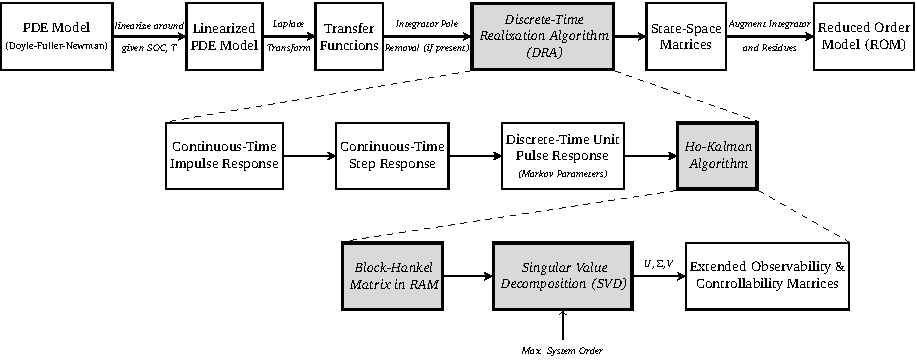
\includegraphics[width=\textwidth]{traditional_dra.pdf}
    \caption[%
    \glsfmtshort{rom} workflow using classical \glsfmtshort{dra}.
    ]%
    {%
        \glsfirst{rom} workflow using classical
        \glsfirst{dra}. The shaded blocks represent computational bottlenecks.
    }%
    \label{fig:traditional_ROM_Workflow}
\end{figure}

\subsection{Size of the Block-Hankel Matrix}\label{sec:size-of-the}

Large Block-Hankel matrices can occur in \gls{dra} computation due to the
following reasons.
\begin{enumerate}
    \item
        For  a  given   duration  of  Markov-parameter  recording,   if  a  high
        sample-rate   \gls{rom}  is   desired,   the   emulation  frequency   in
        the   \gls{dra}  scheme   has   to  be   proportionately  increased   to
        accurately  compute  the continuous-time  step  and  pulse responses  in
        \cref{fig:traditional_ROM_Workflow}. This implies  that the total number
        of time-samples~$N$  for each  Markov parameter will  have to  be scaled
        linearly to  capture the  desired duration  of the  unit-pulse response.
        However,  the size  of the  Block-Hankel matrix  has a  \emph{quadratic}
        dependence on the Markov parameter length.
    \item
        The  recorded sample  size~$N$ could  also  become large  if the  Markov
        parameters of just  one of the transfer functions decay  very slowly. In
        Li-ion batteries, diffusion  within the solid particle  is typically the
        slowest process.  For the cell  modelled in Lee~\etal{},  the unit-pulse
        response of surface concentration of Li adjacent to the positive current
        collector  requires approximately  16000~samples before  reducing to  an
        appreciably low value, as shown in \cref{fig:markov_cse_pos}.
    \item
        For  a  battery  modelling   problem  consisting  of  multiple  transfer
        functions,  the  number  of  entries in  the  Block-Hankel  matrix  also
        scales linearly  with the  number of transfer  functions. Thus,  if more
        cell  variables (\eg{}  concentrations and  potentials at  other spatial
        locations  within the  cell) are  to be  studied, then  the size  of the
        transfer function vector  and that of the  Block-Hankel matrix increases
        correspondingly.
\end{enumerate}

\begin{figure}[!htbp]
    \centering
    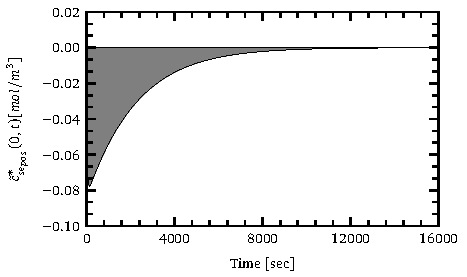
\includegraphics{markov_decay.pdf}
    \caption[Markov parameters of solid surface concentration at positive
    current collector]{Time evolution of Markov parameters of pole-removed transfer
        function corresponding to surface concentration of Li in the solid particle
    adjacent to positive current collector.}
    \label{fig:markov_cse_pos}
\end{figure}

Considering the combined  influence of these effects, if  $x$ transfer functions
are to  be modelled  and $N$  time-samples of  each Markov  parameter are  to be
captured, the corresponding size of the Block-Hankel matrix~$H$ is
\begin{equation}
    \text{Size}(H)\sim \mathcal{O}(x N^2)\text{ entries}
\end{equation}

This    has    a    significant     computational    impact    as    shown    in
\cref{subsec:Traditional-DRA--Memory} and \cref{subsec:Traditional-DRA--CPU}.

\subsection{Classical \glsfmtshort{dra} --- Memory (\glsfmtshort{ram}) Requirements}\label{subsec:Traditional-DRA--Memory}

Lee~\etal~\cite{Lee2012a}  modelled 28~transfer  functions representing  various
electrochemical  variables at  the current  collector and  separator interfaces.
Each Markov  parameter is  a 28~element  column vector.  16000~time-samples were
obtained at  a sample-rate of  \SI{1}{\hertz}, allowing sufficient time  for the
Markov parameters of  the slowest dynamics \ie{} solid  surface concentration to
settle to an  acceptably low magnitude. The Block-Hankel matrix  thus formed has
8000~blocks,  each  block  consisting  of 28~elements  \ie{}  has  $8000  \times
28=224000$~rows  and 8000~columns.  Hence,  the overall  number  of elements  in
the  Block-Hankel  matrix is  $224000  \times  8000=1.79 \times  10^{9}$.  Using
double-precision  arithmetic, its  storage requirement  can be  estimated to  be
\approx \SI{27}{\giga\byte}.

Computing the \gls{svd} results in the formation of three more large matrices in
memory ---
\begin{enumerate*}[label=\roman*)]
    \item matrix   of   output  singular   vectors~$U$,
    \item matrix of  input  singular vectors~$V$, and
    \item the diagonal singular-value  matrix~$\Sigma$.
\end{enumerate*}
With  8000~Hankel-blocks,  approximately  \SI{81}{\giga\byte}  of  \gls{ram}  is
required for holding these three output  matrices generated by a full \gls{svd}.
However,  the  intermediate  operational   memory  usage  during  the  \gls{svd}
computation is often much higher than the  combined size of all the matrices. As
these large  matrices must  be repeatedly  handled for  each operating  point of
\gls{soc} and  temperature, the  high memory demand  of the  classical \gls{dra}
remains a persistent issue.

\subsection{Classical \glsfmtshort{dra} --- \glsfmtshort{cpu} Operation Count}\label{subsec:Traditional-DRA--CPU}

The most  widely used numerical  algorithm for  computing the full  \gls{svd} of
a  generic  dense  matrix $\mbox{\ensuremath{A\in\mathbb{R}^{m  \times  n},m\geq
n}}$  is  the  two-stage  Golub-Kahan-Reinsch  method~\cite{Golub2013}.  In  the
first  stage $A\in\mathbb{R}^{m  \times n}$  is reduced  to an  upper bidiagonal
form.  In  the  second  stage,   \gls{svd}  of  this  upper  bidiagonal  matrix,
$B\in\mathbb{R}^{m  \times n}$  is computed  using an  iterative procedure  such
as  the Demmel-Kahan  method~\cite{Golub2013}. If  stage~\romanletter{1} of  the
\gls{svd}  computation employs  $\mathbb{R}$-Bidiagonalisation~\cite{Golub2013},
then the overall  process is referred to as $\mathbb{R}$-\gls{svd}.  This is the
fastest known  full \gls{svd}  computation method  that may  be applied  to this
battery modelling problem. The \textsc{dgesvd} algorithm, originally implemented
in  \textsc{LAPACK}~\cite{Anderson1999},  employs  this method.  This  has  been
ported to  many numerical computation  packages such  as MATLAB, GNU  Octave and
Scilab.  Several  numerical  libraries  such  as NAG  and  Intel  MKL  also  use
the  \textsc{dgesvd}  codes  due  to its  acclaimed  stability,  robustness  and
versatility.  The MATLAB  implementation `\texttt{\textbf{svd}}'  is also  based
upon \textsc{dgesvd} and  hence this can be considered as  the de-facto baseline
\gls{svd} code.

The    operation    count    for    computing   the    singular    values    and
vectors   of  a   generic   dense  matrix   $\mbox{\ensuremath{A\in\mathbb{R}^{m
\times   n},m\geq    n}}$   using    the   $\mathbb{R}$-\gls{svd}    method   is
$\mbox{\ensuremath{4m^{2}n+22n^{3}}}$~\cite{Golub2013}.  Markov   parameters  of
$x$~transfer functions  and $N$~time-samples  yields a Block-Hankel  matrix with
$m=x N$ rows and $n=N$ columns. Hence,
\begin{alignat}{2}
    \text{\glsfmtshort{cpu} Operation  Count} & = & \,4\left(xN\right){}^{2}N+22N^{3}\nonumber \\
                                              & = & \,2N^{3}\left(11+2x^{2}\right)\label{eq:cpu_op_count}
\end{alignat}
Thus  the \gls{cpu}  operation  count scales  as  $\mathcal{O}(N^{3})$ with  the
number of Markov time-samples~$N$ and as $\mathcal{O}(x^{2})$ with the number of
transfer  functions~$x$ being  modelled. The  \gls{rom} computed  in Lee~\etal{}
uses  28~transfer functions  wherein  the Markov  parameters  are collected  for
\SI{16000}{\second}  with  a sampling  interval  of  \SI{1}{\second}. Thus,  the
\gls{cpu}  operation  count for  performing  this  computation is  approximately
$\mathcal{O}(16000^{3})\approx 4 \times 10^{12}$ floating point operations.

\subsection{Summary Effect of Computational Bottlenecks}\label{subsec:Summary-Effect-of}

The computational bottleneck in a  classical \gls{dra} implementation arises due
to the  requirement of capturing a  large number of Markov  parameters, which in
turn leads  to growth in  Block-Hankel size. In  the case of  battery modelling,
this can arise in the following real-life scenarios:
\begin{enumerate}
	\item
        Electrochemical variables at additional locations of interest within the
        cell (\eg{}  middle of electrode or  separator domain) might need  to be
        modelled. This increases the number  of transfer functions and hence the
        number of Markov parameters.
	\item
        High frequency load  cycles necessitate higher sample-rates  to obtain a
        high fidelity  model. This leads  to a correspondingly higher  number of
        Markov parameters.
	\item
        In cells with  large particle sizes and small  diffusion coefficients, a
        large set  of Markov  parameters is  needed to  capture the  full system
        dynamics.
\end{enumerate}
Lack  of  specialised  computing infrastructure  necessitates  early  truncation
of  the  Markov parameters  in  the  \gls{rom}  workflow. The  resulting  errors
in  the singular  value  computation  lead to  significant  modelling errors  in
the  physical  variables of  the  cell.  Thus,  in practice,  the  computational
bottlenecks of classical \gls{dra} manifest as modelling errors when implemented
in  a  resource-constrained  computing environment.  Furthermore,  this  tedious
computation has to be repeated for multiple \glspl{soc} and temperatures.

The foregoing analysis  clearly demonstrates that the high  memory and \gls{cpu}
demands in  a classical \gls{dra}  implementation severely hamper the  scope and
applicability  of the  reduced order  modelling process.  This implies  that the
modelling  workflow is  not accessible  to research  groups without  specialised
computing infrastructure and its universal  appeal is rendered questionable. The
shaded  blocks in  \cref{fig:traditional_ROM_Workflow}  depict the  hierarchical
propagation of the classical \gls{dra}'s computational bottleneck throughout the
\gls{rom} workflow.

\section{Improved \glsfmtshort{dra} for Battery Modelling}\label{sec:Efficient-Computation-of}

Collecting a  large Markov parameter  set is  inevitable due to  the fundamental
physics of the cell  dynamics as established in \cref{subsec:Summary-Effect-of}.
Hence, in  order to circumvent the  high computational demands of  the classical
\gls{dra}, the second step in the process \ie{} forming the Block-Hankel matrix,
is critically examined with the following scientific rationale.

\begin{enumerate}
	\item
        The unit-pulse responses of most  battery transfer functions (other than
        those of rate-limiting  steps such as solid  diffusion) decay relatively
        quickly. Hence it is inefficient to  record the Markov parameters of the
        full  system for  the  entire  duration needed  to  capture the  slowest
        dynamics.
	\item
        The Block-Hankel  matrix is essentially redundant  information since its
        entries are simply the Markov parameters arranged in a repeating special
        structure. Thus,  it is wasteful to  construct this huge matrix.  If the
        \gls{svd} operation  can be  performed on a  virtual Hankel  matrix, the
        memory requirements can be drastically reduced.
	\item
        The matrix of singular values~$\Sigma$ is diagonal and hence, sparse. It
        is redundant to hold all the non-diagonal entries (zeros) in memory.
	\item
        It  is not  necessary to  perform a  \emph{full} \gls{svd}  operation in
        order  to  achieve order  reduction.  When  an  upper bound  on  desired
        system order  can be  decided a  priori, it is  sufficient to  compute a
        \emph{truncated} \gls{svd}  yielding the first few  dominant triplets of
        $U, \Sigma \text{ and } V$.
\end{enumerate}
Thus,  forming the  large Block-Hankel  matrix  and computing  its \gls{svd}  is
identified as an avoidable bottleneck in the classical \gls{dra}method. This can
be  tackled since  forming the  Block-Hankel matrix  is an  idiosyncrasy of  the
algorithm  used  and  does  not  arise from  any  fundamental  physical  limits.
Facilitated  by  an  efficient  \gls{svd}  implementation,  this  thesis  author
proposes  an improved  \gls{dra}that  serves  as a  drop-in  replacement in  the
\gls{rom} workflow.

\subsection{Candidate Schemes for Block-Hankel \glsfmtshort{svd}}

Generic  \gls{svd}  routines  such  as \textsc{dgesvd}  do  not  take  advantage
of  the  anti-diagonal  structural  symmetry  of  Block-Hankel  matrices.  Since
it  is sufficient  to  obtain  the first  few  leading  eigentriplets for  order
reduction,  iterative  algorithms  such  as   the  Jacobi  and  Lanczos  schemes
(see~\cite{Golub2013})  emerge  as  attractive candidates  for  computing  these
dominant singular  values and vectors. In  order to ensure accessibility  to the
large community of  battery researchers and to encourage  widespread adoption of
the fast reduced order modelling framework, the author of this thesis considered
only freely available  open-source numerical libraries that exist  in the public
domain, especially  those with permissive  licensing terms. Otherwise  the gains
achieved by  an efficient  \gls{svd} computation  for implementing  \gls{dra} on
non-specialised  computing  hardware would  be  offset  by commercial  licensing
terms,  usage restrictions  and  monetary considerations  associated with  using
proprietary  codes. Among  these  open-source candidate  algorithms, the  Jacobi
scheme~\cite{Golub2013} is  available through the  xGESVD routine in  the LAPACK
suite~\cite{Anderson1999}. FORTRAN 77 codes for the implicitly restarted Arnoldi
and Lanczos schemes~(see~nu-TrLan~\cite{Yamazaki2008}) are  available as part of
the ARPACK~\cite{Lehoucq1998} library.

The practical drawback  of most \gls{svd} implementations,  both open-source and
proprietary, is  that they require  the entire  matrix as input  argument. Since
operating upon  the Block-Hankel  matrix requires constructing  it in  the first
place, the memory bottlenecks discussed in \cref{subsec:Traditional-DRA--Memory}
are not  ameliorated. An  example is  the \texttt{svds}  routine ---  an economy
size  \gls{svd}  implementation  in  MATLAB\@.   Albeit  this  is  a  commercial
implementation  of  the  Arnoldi  codes,  any potential  benefits  of  using  an
iterative scheme is nullified by the memory penalty. Owing to reasons enumerated
in \cref{sec:Efficient-Computation-of}, the chosen  \gls{svd} algorithm needs to
be able to handle the computation without actually forming the huge block-Hankel
matrix in memory.

\subsection{\glsfmtshort{svd} Operation on a Virtual Block-Hankel Matrix}

The  pioneering  work  by  Larsen, PROPACK~\cite{LarsenPropack},  based  on  his
earlier work~\cite{Larsen1998} implements a numerically stable Lanczos \gls{svd}
computation designed specifically for large  and sparse matrices. In addition to
the ability  to operate on the  matrix as a  whole, the PROPACK codes  possess a
unique flexibility  of accepting  input arguments  in a  functional form.  A key
highlight of the  Lanczos \gls{svd} scheme is that it  does not strictly require
the  matrix  itself, but  only  the  product of  the  matrix  and its  transpose
with  an  arbitrary vector.  This  feature  has  been effectively  exploited  in
the  PROPACK suite.  Therefore, these  multiplication routines  can be  supplied
as  input  arguments instead  of  forming  the  large Block-Hankel  matrices  in
memory.  Furthermore,  this  package  includes  sophisticated  schemes  such  as
Gram-Schmidt  partial re-orthogonalisation~\cite{Bjorck1994}  to compensate  for
numerical round-off  errors in the  basic Lanczos bidiagonalisation  and ensures
orthogonality of  the input and  output singular  vectors. The PROPACK  suite is
available as both Fortran~77 and MATLAB codes distributed under a permissive BSD
license. Version~1.1 of the MATLAB implementation  of the PROPACK suite was used
by this thesis author.

For the \gls{rom} workflow, in order  to use PROPACK's unique feature \viz{} its
flexibility to  accept functional form  inputs, the key  is to use  an algorithm
that  effectively  exploits the  affine  structure  of the  Block-Hankel  matrix
without  actually  forming  it  in  memory. Recent  research  in  a  specialised
time-series technique known as \gls{ssa}~\cite{Elsner1996} has yielded efficient
methods for  achieving this goal.  Korobeynikov~\cite{Korobeynikov2010} proposed
an  algorithm that  employs the  \gls{fft} for  implementing this  matrix-vector
product  by  embedding the  Markov  parameters  into  the  column vectors  of  a
circulant  matrix.  This  is  suitable   for  applications  wherein  the  Hankel
matrix  is  composed  of scalar  entries  such  as  that  formed by  the  Markov
parameters  of   a  \gls{siso}   transfer  function.  Golyandina,   Usevich  and
colleagues~\cite{Golyandina2010,Golyandina2015}  extended  this  approach  to  a
generic  2D-case for  performing \gls{ssa}  on images.  With this  modification,
this  algorithm is  rendered capable  of handling  the structure  of Multi-level
Block-Hankel matrices formed from the  Markov parameters of a generic \gls{mimo}
system. While  the modified  scheme does not  construct the  Block-Hankel matrix
in  memory,  the operational  rubrics  of  the Golyandina-Usevich  algorithm  in
conjunction with  PROPACK is  such that  they iteratively  operate on  a virtual
Hankel matrix  of equivalent size.  The Golyandina-Usevich algorithm  is briefly
summarised in \cref{sec:Golyandina-Usevich-Algorithm}.

\section{Golyandina-Usevich Algorithm\label{sec:Golyandina-Usevich-Algorithm}}

The  Golyandina-Usevich  algorithm  is  used  for computing  the  product  of  a
Block-Hankel matrix with an arbitrary vector.  The steps involved in this scheme
are enumerated  in Algorithm~3 of  Golyandina~\etal~\cite{Golyandina2015}. These
steps are reproduced  here in the context of the  improved \gls{dra} for reduced
order battery modelling.

\begin{enumerate}
	\item Compute a 2-D \gls{fft} of Markov parameter matrix.
	\item Form an augmented vector by zero-padding the arbitrary vector input
	    from Lanczos iteration.
	\item Perform a column-wise reshaping of this augmented vector to obtain
	    a new matrix with the same dimensions of the Markov parameter matrix.
	\item Compute the element-wise product of this newly created matrix with
	    the 2-D \gls{fft} of Markov parameter matrix.
	\item Reshape the resulting matrix back to a column vector.
	\item Extract the first $L$ elements from this vector, wherein $L=K x$.
	    $K$ represents the desired block-Hankel size and $x$ represents
	    the number of transfer functions being modelled.
\end{enumerate}

At the end of  Step~6, the product of the Hankel matrix  and arbitrary vector is
obtained. This is  reused as an input  for the Lanczos scheme  which generates a
new arbitrary vector  in the subsequent iteration. Thus, the  steps 1--6 are run
in a loop within the main Lanczos scheme.  These same steps can also be used for
computing the  product of the transpose  of the Hankel matrix  and the arbitrary
vector.  The only  change is  to  account for  the different  dimensions of  the
arbitrary  vector input  from  the  Lanczos scheme  in  step~2.  As a  practical
implementation, software code representing steps 1--6 is written in a plain-text
file and used  as functional-form inputs by the PROPACK  scheme which implements
the Lanczos iteration.

\section{Customisations for Battery Modelling}

Specific considerations  are required  for incorporating  the Golyandina-Usevich
algorithm  in  the  \gls{rom}  workflow  for  Li-ion  batteries.  The  classical
\gls{dra}  architecture is  set up  to  handle \gls{simo}  systems, wherein  all
transfer functions  are derived by  considering only  a single input  \viz{} the
applied battery  current. Thus  the Markov parameters  form a  2D~matrix wherein
each  row corresponds  to  individual battery  transfer  functions with  columns
representing  unit-pulse  response  samples  for  each  transfer  function.  The
2D~moving-window  illustrated in~\cite{Golyandina2015}  for Block-Hankel  matrix
formulation has to be suitably reshaped to account for this structure. Step~3 of
the  algorithm  deals  with  2-D~\gls{fft}  computation  of  the  \gls{mpm}.  In
this  thesis author's  implementation,  this is  pre-computed  since it  remains
invariant between iterations of the Hankel-vector product computation loop. This
pre-allocation and a~priori computation contributes to overall code efficiency.


\begin{figure}[!htbp]
    \centering
    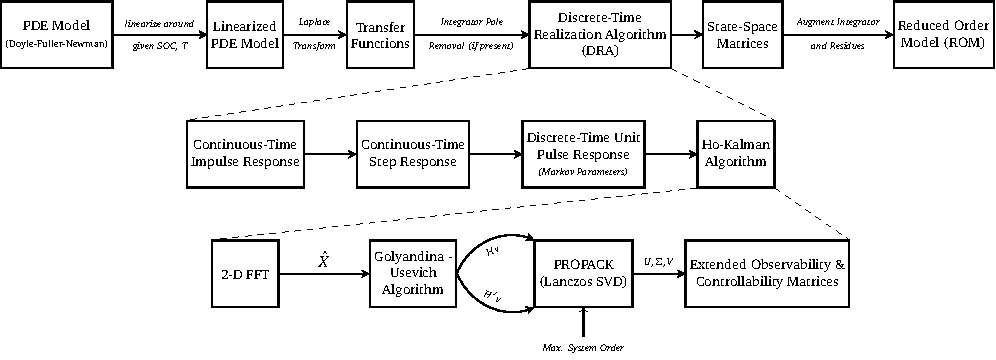
\includegraphics[width=\textwidth]{new_rom.pdf}
    \caption[%
    \glsfmtshort{rom} workflow using improved \glsfmtshort{dra}
    ]%
    {%
        \glsfirst{rom} workflow using improved \glsfirst{dra}.
    }%
    \label{fig:improved_ROM_workflow}
\end{figure}

\Cref{fig:improved_ROM_workflow} shows the \gls{rom}  workflow with the improved
\gls{dra} wherein all computational bottlenecks  highlighted by shaded blocks in
\cref{fig:traditional_ROM_Workflow}  have been  eliminated. The  strategy is  to
first employ the (suitably modified) Golyandina-Usevich algorithm for describing
the matrix-vector  multiplication routines.  These two  functions are  then used
as  inputs  to  the  PROPACK  codes.  Eigentriplets  up  to  the  desired  upper
bound on  system order  is then  computed using  a Lanczos  \gls{svd} iteration.
\Cref{fig:svdcompare} presents a comparison of  singular values computed by both
the  traditional and  new methodologies.  It  is evident  that the  two sets  of
singular values are identical. This proves  that the new scheme can indeed serve
as a drop-in replacement for the classical \gls{dra}.

\begin{figure}[!htbp]
    \centering
    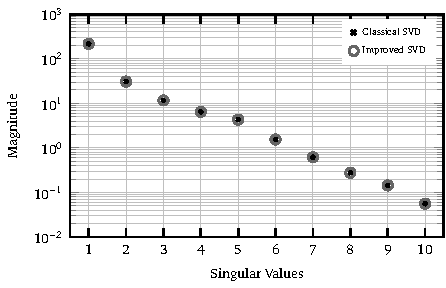
\includegraphics{svd_compare.pdf}
    \caption[Singular values computed by conventional and
    improved \glsfmtshort{svd} methods]{Comparison of singular values computed by the conventional and
        improved \glsfmtshort{svd} methods. Using the new scheme results in
    identical singular values}
    \label{fig:svdcompare}
\end{figure}

\section{Simulation Results and Discussion}\label{sec:Results}

This section provides a quantitative  demonstration of the reduced computational
demand  of the  improved \gls{dra}  scheme by  comparing it  with the  classical
\gls{dra}implementation. The  physical parameters  of the cell  are the  same as
those published in  Fuller~\etal~\cite{Fuller1994}. \Cref{table:simparams} lists
the  parameters used  in  the  \gls{rom} workflow  (same  as  those employed  by
Lee~\etal~\cite{Lee2012a}).

\begin{table}[!htbp]
    \centering
    \caption{Parameters for \gls{rom} Computation}
    \label{table:simparams}
    \begin{tabular}{@{} l l @{}}
        \toprule
		Initial Cell \glsfmtshort{soc}             & \SI{60}{\percent} \\
		Hankel Block Size                          & 8000              \\
		Discrete-Time Model Sample-Rate,~$T_s$     & \SI{1}{\second}   \\
		Number of Electrolyte EigenModes           & 5                 \\
		Continuous-Time Emulation Frequency,~$F_1$ & \SI{128}{\hertz}  \\
		Desired Number of Singular Values          & 10                \\
		\bottomrule
    \end{tabular}
\end{table}

\Cref{fig:memory}  shows a  comparison  of  the memory  usage  of classical  and
improved \gls{dra} methods.  It is evident that the \gls{svd}  step in classical
\gls{dra}  consumes  an  overwhelming  majority  of  the  total  memory  demand,
requiring \approx \SI{100}{\giga\byte} for a Hankel block size of~8000. This can
be a limiting factor  in modelling slow cell dynamics without  access to a large
memory workstation. The improved \gls{dra} method eliminates this bottleneck and
the memory  usage of \gls{svd} step  is negligible. Overall memory  usage of the
improved  \gls{dra} is  dominated by  Markov parameter  computation. Considering
\SI{10}{\giga\byte} of usable \gls{ram}, this means that 60000~Markov parameters
(Hankel Block-size of~30000) can be captured.

\begin{figure}[!htbp]
    \centering
    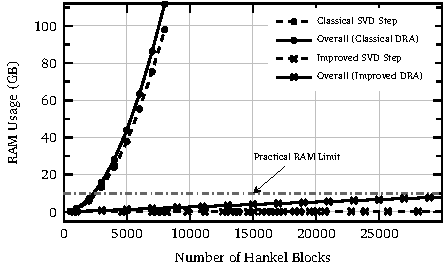
\includegraphics{ram_usage.pdf}
    \caption[%
    Memory usage of classical and improved \glsfmtshort{dra}
    ]%
    {%
        Memory  usage  of  classical and  improved  \glsfmtshort{dra}.  Overall,
        \glsfmtshort{ram}  usage   as  well   as  the   memory  used   only  for
        \glsfmtshort{svd} computation is illustrated.
    }%
    \label{fig:memory}
\end{figure}

\Cref{fig:cputime}  shows   a  comparison  of  \gls{cpu}   times  for  computing
the   \gls{rom}  at   a  single   \gls{soc}   and  temperature   for  both   the
classical  and  the improved  \gls{dra}  methods\footnote{\label{fn:clusterspec}
All  computations  reported  in  this  chapter were  performed  on  a  dedicated
high-\glsfmtshort{ram}  pool  drawn  from  the compute  cluster  hosted  at  the
Department  of  Mathematics at  Imperial  College  London.  The author  of  this
thesis  wishes  to   express  his  thankfulness  to   the  relevant  authorities
for  providing  access  to  this  facility.  The  resources  borrowed  were  one
core  of  a  \mbox{4-core}  \mbox{\text{Intel}\textsuperscript{\textregistered}}
\mbox{Xeon\textsuperscript{\textregistered}} \mbox{E5-2637~v3} processor clocked
at   \SI{3.50}{\giga\hertz}   with   \SI{500}{\giga\byte}   \glsfmtshort{ram}.}.
Owing   to   the   high   operation  count   for   the   \gls{svd}   computation
(see   \cref{eq:cpu_op_count}),  the   classical   \gls{dra}  requires   \approx
\SI{40}{\minute} for a Hankel block size of~8000. Clearly, the overall \gls{cpu}
time for the  classical \gls{dra} is almost exclusively spent  for computing the
\gls{svd}. The improved \gls{dra} method  reduces the overall computational time
by  two  orders of  magnitude,  taking  \approx  \SI{40}{\second} for  the  same
block-size.  In this  case,  the  \gls{cpu} time  is  evenly  split between  the
\gls{svd} and Markov parameter computations.

\begin{figure}[!htbp]
    \centering
    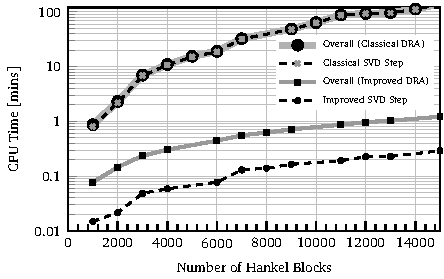
\includegraphics{cpu_usage.pdf}
    \caption{Computation times for classical and improved \glsfmtshort{dra} schemes}
    \label{fig:cputime}
\end{figure}

From  \cref{fig:memory},   it  is  evident   that  if  classical   \gls{dra}  is
employed,  a  standard  laptop  with  a  nominal  \SI{10}{\giga\byte}  \gls{ram}
limit   (dedicated   for   \gls{rom}   workflow)   cannot   capture   the   full
cell   dynamics  and   hence   is  restricted   to   2500~Hankel  blocks.   This
necessitates early  truncation of Markov parameters  at \SI{5000}{\second}. From
\cref{fig:markov_cse_pos}, the truncation residue  at \SI{5000}{\second} for the
unit-pulse response of solid surface concentration at positive current collector
is $\SI{-0.0087}{\mole\per\meter\cubed}$. The truncation errors in the \gls{mpm}
directly translate  to errors in  computed singular values,  adversely affecting
accuracy of  simulated cell  variables. It  must be noted  that the  accuracy of
simulation results  reported here  does not  bear a  causal relationship  to the
particular  \gls{dra} scheme  employed. In  principle,  when an  upper bound  on
computational usage has not been enforced,  the numerical operations of both the
existing and proposed \gls{dra} schemes lead to similar error magnitudes for the
modelled quantities. Instead, the accuracy comparison illustrated here primarily
serves to demonstrate the practical  usefulness of the improved \gls{dra} scheme
when implemented in a commonplace computing environment.

\Cref{fig:truncated}  shows a  comparison  of singular  values  obtained by  the
classical and improved \gls{svd} methods  computed by imposing a \gls{ram} limit
of \SI{10}{\giga\byte}. Owing to early truncation of the \gls{mpm}, the dominant
singular values  computed by the  conventional method differ  significantly from
those computed by the improved \gls{svd} operating on untruncated data. With the
same memory  constraints, the improved  \gls{dra} can handle up  to 30000~Hankel
blocks, allowing for capture of \SI{60000}{\second} of Markov parameter data.

\begin{figure}[!htbp]
    \centering
    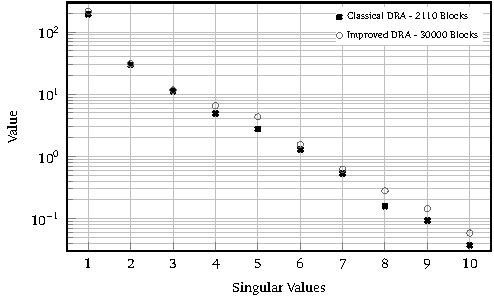
\includegraphics{truncated.pdf}
    \caption{Comparison of singular values computed by conventional and improved
        \glsfmtshort{svd} methods under a practical \glsfmtshort{ram} limit of
    \SI{10}{\giga\byte}}
    \label{fig:truncated}
\end{figure}

For comparative analysis  of modelling accuracy under this  memory constraint, a
time-domain simulation  of the  \glspl{rom} obtained  by classical  and improved
\gls{dra}  methods is  performed.  The input  current  profile corresponding  to
a  \gls{udds}  drive  cycle  reported in  Lee~\etal{}~\cite{Lee2012a}  is  used.
\Cref{fig:time_domain_sim}  depicts  the  time-evolution of  the  solid  surface
concentration  at  the  positive  electrode/separator  boundary.  For  comparing
the  accuracy   of  the   two  ROMs,  a   COMSOL  Multiphysics~\cite{COMSOL2012}
simulation  of  the  full-order   pseudo-2D  porous-electrode  \gls{pdae}  model
is  used  as   the  reference.  The  \gls{rom}   employing  classical  \gls{dra}
diverges  over   time,  and  after   \SI{1500}{\second}  results  in   an  error
of  \SI{1120}{\mole\per\meter\cubed}.   The  \gls{rom}  incorporating   the  new
\gls{dra}  workflow   accurately  tracks   the  COMSOL   simulation  trend-line.

\begin{figure}[!htbp]
    \centering
    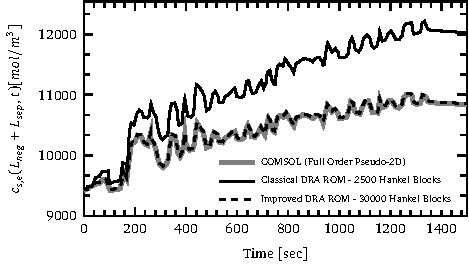
\includegraphics{comsol_comparison.pdf}
    \caption[%
    Evolution of solid surface concentrations at
    positive electrode/separator interface.
    ]%
    {%
        Time-domain  simulation depicting  solid surface  concentrations at  the
        boundary  of positive  electrode and  separator. The  simulation results
        from  the  \gls{p2d}  model  implemented   in  COMSOL  is  used  as  the
        reference  benchmark. The  two  \glsfmtshortpl{rom}  were derived  under
        a  \glsfmtshort{ram}  limit   of  \SI{10}{\giga\byte}.  The  performance
        of  the  improved \glsfmtshort{dra}  is  significantly  better than  the
        classical \glsfmtshort{dra} owing to the  fact that its derivation could
        accommodate  a larger  number  of Hankel  blocks  without exceeding  the
        specified memory limit.
    }%
    \label{fig:time_domain_sim}
\end{figure}

\Cref{tbl:salientresults}   provides   a   summary   of   the   key   simulation
results.  At  a  single  operating  point  of  \gls{soc}  and  temperature,  for
a  Hankel  block   size  of~8000,  the  \gls{rom}   workflow  incorporating  the
improved  \gls{dra}  is  \approx  100  times  faster  than  that  employing  the
classical   \gls{dra}.  Using   the  machine   with  specifications   listed  in
the  footnote\textsuperscript{\ref{fn:clusterspec}},  for  100~operating  points
(combinations of  10~\gls{soc} and temperature values),  computing the \gls{rom}
requires  only  6~hours using  the  improved  \gls{dra}, whereas  the  classical
\gls{dra} consumes  666~hours (27~days).  Furthermore, for the  same block-size,
the  improved \gls{dra}  is  demonstrated  to be  superior  in  terms of  memory
efficiency,  drastically reducing  the memory  requirement from  112~GB down  to
2~GB. Finally,  the improved \gls{dra} demonstrates  superior modelling accuracy
when  implemented even  in moderately  equipped computing  environments such  as
laptops.

\begin{table}[!htbp]
	% \singlespacing
	\centering
	\caption{Salient Results --- Classical vs.\ Improved \gls{dra} }
	\label{tbl:salientresults}
	\setlength{\extrarowheight}{1pt}
	\begin{tabular}{ @{} l c l l @{} }
		\toprule
		% \gls{rom}                                & Quantity                                & Classical                                   & Improved                                  \\
		% Condition                                &                                         & \gls{dra}                                   & \gls{dra}                                 \\
		\makecell{\gls{rom} \\ Condition} & {Entity} & \makecell{Classical \\ \gls{dra} } & \makecell{Improved \\ \gls{dra}} \\
		\midrule
		\multirow{8}{1.22cm}{8000 Hankel Blocks} & Memory                         & 111.80 GB                        & 2.14 GB                        \\ [-5pt]
                                                 & \footnotesize (overall)        &                                  &                                \\
                                                 & Memory                         & 97.93 GB                         & 0.03 GB                        \\ [-5pt]
                                                 & \footnotesize(\gls{svd} step)  &                                  &                                \\
                                                 & \gls{cpu} Time                 & 39.78 min                        & 0.63 min                       \\ [-5pt]
                                                 & \footnotesize(overall)         &                                  &                                \\
                                                 & \gls{cpu} Time                 & 39.30 min                        & 0.14 min                       \\ [-5pt]
                                                 & \footnotesize(\gls{svd} step)  &                                  &                                \\ [2.5pt]
		\midrule
		\multirow{3}{1.22cm}{10 GB Memory Limit} & Block Size                     & 2500                             & 30000                          \\ [5pt]
                                                 & Max.\ error                    & \SI{1120}{\mole\per\meter\cubed} & \SI{13}{\mole\per\meter\cubed} \\ [-5pt]
                                                 & in $c_{{s,e}_\text{pos}}(1,t)$ &                                  &                                \\ [5pt]
		\bottomrule
	\end{tabular}
\end{table}

% The  proposed  method opens  up  the  possibility  of modelling  other  physical
% quantities  in  the   cell's  geometry  without  being   hindered  by  computing
% limitations. Furthermore, high sample-rate models  to handle highly dynamic load
% profiles  can be  deployed in  future  \gls{bms} applications.  The scheme  also
% empowers the \gls{rom} framework to tackle  cells with slower dynamics and other
% chemistries  with different  rate-limiting  mechanisms.  The improved  \gls{dra}
% method therefore  opens up a  wide range of  possibilities and looks  capable of
% bringing  the goal  of  physics-based  battery model  implementation  in a  high
% performance real-time \gls{bms}, a step closer to realisation.

% Despite   the  aforementioned   euphoric   possibilities   facilitated  by   the
% streamlining  of  the reduced  order  modelling  workflow through  the  improved
% \gls{dra},  there  exists a  fundamental  deficiency  in this  hybrid  modelling
% approach  that impede  its  effective deployment  as the  plant  model in  state
% estimation tasks. This aspect was already discussed in \cref{ch:littreview}, and
% is  reiterated here.  The  entries in  the  matrices of  the  final state  space
% model  depend on  the linearisation  point  of \gls{soc}  and temperature.  This
% linearisation requirement adversely affects the usability of the model for state
% estimation tasks, wherein the \gls{soc} is in fact an unknown quantity and is to
% be  estimated.  This  cyclic  dependency between  the  linearisation  point  and
% the  state-estimation quantity  makes  the  use of  this  model questionable  in
% a  demanding  application such  as  in  embedded \glspl{bms}  on-board  electric
% vehicles.

This  chapter  concludes  with  the  view  that,  although  the  bottlenecks  in
Lee~\etal~\cite{Lee2012a}  revealed   by  this   in-depth  analysis   have  been
effectively tackled  in this chapter,  owing to the circular  dependency between
the linearisation point and model parameters, the underlying model itself is not
robust enough for immediate implementation. Furthermore, the model derivation is
convoluted  with the  derivation being  performed  in the  frequency domain  and
implementation in the  time-domain. This thesis author is of  the opinion that a
simple, yet  accurate model derived  and implemented entirely in  time-domain is
the  need  of  the  hour  for  encouraging  the  automotive  industry  to  adapt
physics-based battery models onto on-board  \glspl{bms} of electric vehicles. In
the quest to  fulfil this need, an analysis of  the simplest time-domain physics
based model \viz{} the \gls{spm} is presented next in \cref{ch:spmanalysis}.
                   % Improved DRA
\setcounter{chapter}{4}
% -*- root: ../../main.tex -*-
%!TEX root = ../../main.tex
% vim:textwidth=80 fo=cqt


\graphicspath{{chapters/spm_analysis/figures/}}
% ----------------------- contents from here ------------------------

\clearpage
\chapter{Performance Evaluation of State of the Art in Single Particle Modelling}\label{ch:spmanalysis}
\startcontents[chapters]
\printcontents[chapters]{}{1}{\setcounter{tocdepth}{1}}

\bigskip

% -*- root: ../../main.tex -*-
%!TEX root = ../../main.tex
% this file is called up by main.tex
% content in this file will be fed into the main document
% vim:textwidth=80 fo=cqt

% The state of the art implementation  for tackling these drawbacks is presented
% and their inadequacies are discussed.

\capolettera{T}{aking} into consideration the  relative strengths and weaknesses
of  all the  physics-based reduced  order modelling  families in  the literature
considered  (see  \cref{ch:littreview}),  the   overarching  simplicity  of  the
\gls{spm}  coupled  with   its  immediate  potential  to  bring   the  power  of
physics-based predictions to  an embedded environment is a  strong motivation to
pursue  an in-depth  exploration of  its  horizons. This  chapter discusses  the
performance of multiple \gls{spm} variants, ranging from basic to sophisticated.
The governing equations  of the conventional \gls{spm} are  first introduced and
its baseline performance  is evaluated. Next, an in-depth analysis  of the basic
\gls{spm}'s drawbacks is performed. Various published attempts to mitigate their
current challenges towards implementability  is presented and their inadequacies
discussed. Owing  to its  simplicity and latent  potential, a  popular modelling
strategy from the existing art that aims to enhance the performance of the basic
\gls{spm} through incorporation  of electrolyte dynamics, is  chosen for further
analysis.  The chapter  concludes with  the  author's critical  comments on  its
relative merits that come to view  through comparison against a benchmark model,
whilst simultaneously  identifying its critical weakness  whose mitigation forms
the focal point of the research discussed in \cref{ch:newelectrolytemodel}.

 % Intro to the SPM analysis chapter

% \section{The conventional \glsfmtfull{spm}}\label{sec:spmintro}
% % -*- root: ../../main.tex -*-
%!TEX root = ../../main.tex
% this file is called up by main.tex
% content in this file will be fed into the main document
% vim:textwidth=80 fo=cqt

% As  discussed in  \cref{sec:classificationscheme},\fxnote{may need  to cross-ref
% the relevant subsection}

Reducing  the number  of  computational  dimensions in  a  physical model  helps
in  formulating  their  low  order  approximations,  thereby  facilitating  fast
evaluations  of  the modelled  quantities.  The  \gls{spm}, originally  used  in
modelling  the Metal-Hydride  chemistry~\cite{Haran1998}  and  later on  adapted
for  Li-ion  cells~\cite{Ning2004},  represents  the canonical  apogee  of  such
dimension-reduction strategies.


During  the  initial years  following  its  inception,  the formulation  of  the
basic \gls{spm}  was discussed extensively within  application-specific contexts
such  as  \gls{soc}  evaluation~\cite{Santhanagopalan2006a,Santhanagopalan2008},
parameter    estimation~\cite{Santhanagopalan2007},   and    life   cycle/ageing
predictions~\cite{Santhanagopalan2008a,Safari2009}.   There   have   also   been
detailed   stand-alone   publications   discussing   various   facets   of   the
basic   \gls{spm},   such   as    its   inherent   assumptions   and   governing
equations~\cite{Santhanagopalan2006,Chaturvedi2010}. The basic \gls{spm} suffers
from  certain major  drawbacks which  are  discussed in  the simulation  results
presented  in \cref{subsec:simresultsbasicspm}.  Since the  turn of  the decade,
researchers  have attempted  to  tackle  many of  these  issues  and a  holistic
discussion of such efforts is presented in \cref{sec:electrolyteinclusion}.

A survey  of the  most recent  literature dealing with  the \gls{spm}  family of
models reveals a diminishing rate of advancement in quantifiable improvements to
the underlying plant model itself. This nearly-static trend can be attributed to
the general  consensus within the  research community  that these models  may be
too  simplistic  and  not  of  suitable accuracy  to  warrant  further  studies.
Other  than a  small  minority  of papers  that  either  propose core  modelling
improvements  to tackle  their inaccuracies,  or  add new  enhancements such  as
mechanical-stress  physics~\cite{Li2017a,Li2018b}, latest  work  in this  family
of  models predominantly  pertains  to  their application  in  areas like  state
estimation~\cite{Chaochun2018,Lin2017,Tran2017,Moura2017,Zou2016a},      optimal
charging~\cite{Perez2017,Perez2017a},    cycling    performance~\cite{Maia2017},
conversion           to            equivalent           circuits~\cite{Li2017b},
parametrisation~\cite{Li2018,Rajabloo2017,Bizeray2017,Namor2017}, pack-balancing
studies~\cite{Docimo2018a}  and   observer  design  for   joint  state-parameter
estimation~\cite{Ascencio2016}. The \gls{spm} approach  was also extended to the
case of  composite electrodes, leading to  a state estimator design  after basic
observablity  analysis~\cite{Bartlett2015}.  Owing  to  their  simplicity,  this
author believes that \glspl{spm} hold the highest potential to bring a \gls{pbm}
to embedded \glspl{bms}. With this goal  in view, this thesis seeks to resurrect
interest in this field by addressing the recent paucity in fundamental modelling
improvements. However, prior to doing  this, a complete analysis identifying the
strengths and  weaknesses of the salient  models within the \gls{spm}  family is
warranted.

% A proposed enhancement to the basic \gls{spm} is the main contribution of this
% author and shall be discussed in \cref{ch:newelectrolytemodel}.



\section{\glsfmtshort{spm} Model Development}\label{sec:spmmodeldevelopment}
% -*- root: ../../main.tex -*-
%!TEX root = ../../main.tex
% vim:textwidth=80 fo=cqt

In  order  to  establish  a  context  for the  author's  work  to  be  discussed
in  \cref{ch:newelectrolytemodel},  it  is  imperative  to  provide  a  holistic
presentation of the basic \gls{spm} modelling art. The conventional \gls{spm} is
the  simplest  of  all  time  domain  \glspl{pbm}.  The  rest  of  this  section
provides  this author's  digested summary  of its  modelling rubrics  based upon
the  keen  insights  gained  from  perusing  the  vanguard  literature  in  this
topic~\cite{Santhanagopalan2006,Santhanagopalan2006a,DiDomenico2010} as  well as
their relevant derivative works.

\subsection{Geometry}\label{subsec:basicspmgeometry}

A  description  of   the  working  principle  of  the  cell   was  presented  in
\cref{subsec:liionchemistry} and  is not  repeated here.  The \gls{spm}  aims to
capture the electrochemical phenomena along the thickness~$l_j$,~\jinnegpos{} of
each  porous electrode  by a  representative  spherical particle.  Thus the  two
distinct  solid  phase porous  regions  of  the  cell \ie~the  negative  and
positive electrode regions, are idealised as two spheres of radii~$R_\text{neg}$
and~$R_\text{pos}$ respectively.


\Cref{fig:sandwichtospm}   shows   the   geometrical  origins   of   the   basic
\gls{spm}.  In  this   arrangement,  the  spatial  dimension   along  the  axial
thickness  of   each  electrode   degenerates  to  a   single  point   which  is
represented  by  a sphere.  Hence,  the  concentration  of lithium  within  each
electrode~$c_{\text{s}_j}$,~\jinnegpos{}  is  only  a  function  of  the  radial
position~$r_j$,~\jinnegpos{}  and  the  time~$t$.   The  surface  area  of  each
representative sphere is scaled appropriately,  such that they are equivalent to
the  active area~$A_\text{elec}$  of the  corresponding  porous electrodes. 
Thus the  \gls{spm} accounts  for  the  reduced  volume-fraction  arising  due 
to  the  microporous structure  of  the   solid  phase  and  hence,  the 
storage   capacity  of  the representative  particles  match  that  of  the 
corresponding  electrodes.  The overarching  assumption  of  the  \gls{spm}
modelling  philosophy  is  that  the electrochemical performance of these
representative electrodes are sufficient to model the voltage behaviour of the
cell at its terminals. The \gls{spm} thus employs the coarsest possible spatial 
discretisation of the cell's thickness  with the goal of minimising
computational burden.

\begin{figure}[!htbp]
    \centering
    \begin{tikzpicture}
        \node[anchor=south west,inner sep=0] (image) at (0,0) {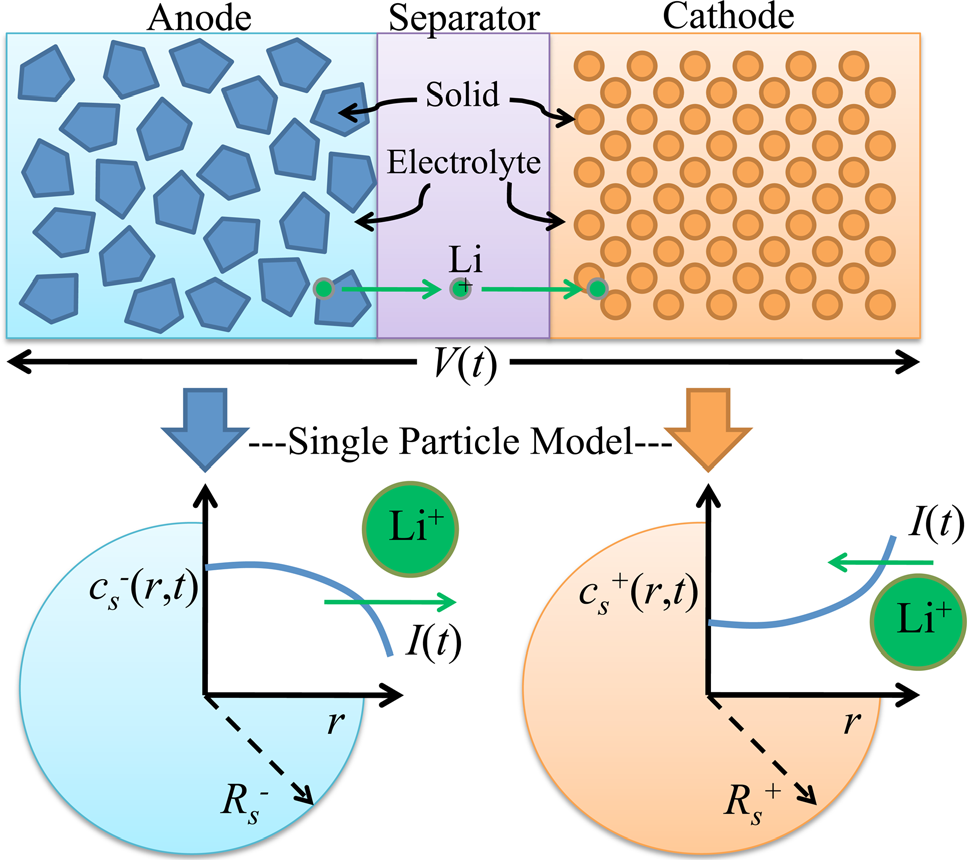
\includegraphics{spm_geometry}};
        \begin{scope}[x={(image.south east)},y={(image.north west)}]
            \node[fill=mourablue,inner sep=0pt,outer sep=0pt] at (0.265,0.045) {\scriptsize $\text{p}_\text{n}$};
            \node[minimum height=3mm, minimum width=2mm,fill=mourablue,inner sep=2pt,outer sep=2pt] at (0.27,0.09) {};
            \node[fill=mouraorange,inner sep=0pt,outer sep=0pt] at (0.785,0.045) {\scriptsize $\text{p}_\text{p}$};
            \node[minimum height=3mm, minimum width=2mm,fill=mouraorange,inner sep=2pt,outer sep=2pt] at (0.80,0.085) {};
        \end{scope}
    \end{tikzpicture}
    \caption[Schematic illustration depicting geometrical origins of the
    \glsfmtshort{spm}]
    {%
        Schematic illustration depicting the geometrical origins of the basic
        \gls{spm}. The model is obtained through a degenerate spatial
        discretisation of one electrochemical layer of a  pouch cell.  The
        active material of each porous electrode is represented by one
        representative spherical particle, thus entirely eliminating the spatial
        dimension along the axial direction. Illustration adapted
        from Moura~\etal~\cite{Moura2012}.
    }%
    \label{fig:sandwichtospm}
\end{figure}

\subsection{Scope and Assumptions}\label{subsec:basicspmassumptions}

Having described the  geometrical representation of the model,  it is imperative
to establish its  aims and scope. This section discusses  the subset of physical
phenomena  that can  be  captured  by the  basic  \gls{spm}  and enumerates  the
inherent assumptions in model derivation.  The validity of these assumptions and
their effects  on model accuracy shall  be examined in the  results presented in
\cref{subsec:simresultsbasicspm}. As  a broad  outline of  its scope,  the model
attributes the cell polarisation to two dominant physics \viz~reaction kinetics
and solid phase transport phenomena \ie~diffusion dynamics.


The  \gls{spm}  assumes that  charge  transfer  happens throughout  the  surface
of  each  representative  spherical  particle where  intercalation  occurs.  The
electronic  conductivity of  the solid  phase is  assumed to  be high  enough to
ignore the spatial distribution  of charge \ie~the local  volumetric current
density is assumed  to be uniform along the thickness  of each porous electrode.
This assumption is  motivated from early calculations by Newman and
Tobias~\cite{Newman1962} in their stand-alone  analysis of current distributions
in porous electrodes, wherein a volume-averaged molar flux was deemed sufficient
throughout  the  thickness  of  the  electrode.  This  uniform  current  density
assumption implies  that all of the  particles in the electrode  active material
are  in parallel.  Solid  phase  diffusion dynamics  within  each electrode  are
therefore solved by assuming this averaged electrochemical reaction rate. In the
simulation study  by Smith and~Wang~\cite{Smith2006},  it is reported  that soon
after  the beginning  of discharge,  solid  phase concentration  and ionic  flux
become nearly  independent of  spatial position, and  that lithium  diffusion in
solid particles may be driven by an averaged molar flux at the surface.


Based  on the  discussion thus  far, it  is clear  that the  \gls{spm} does  not
attempt to  model all  physical processes  within the  cell. In  particular, the
model assumes  instantaneous charge  transport from one  electrode to  the other
through  the  solution  phase.  This  implies  that  electrolytic  diffusion  is
sufficiently  fast  (relative to  diffusion  in  the  solid phase).  Thus,  mass
transport  phenomena  in  the  electrolyte  have been  neglected  in  the  basic
\gls{spm}.


During   the  operation   of  the   cell,   the  \gls{spm}   assumes  that   the
electrolyte  concentration~$c_\text{e}$  remains  constant  at  its  equilibrium
initial value~$c_{\text{e},0}$  throughout the cell thickness.  Neglecting local
concentration gradients in  the solution phase, together with  ignoring its mass
transport phenomena, implies  that the current in the electrolyte  does not vary
over  space  and  time.  Hence,  in  the  conventional  \gls{spm}  there  is  no
contribution of the solution phase  to internal overpotentials \ie~electrolyte
dynamics have  no influence on the  cell's terminal voltage. The  \gls{spm} also
ignores any  variations in material  porosities in each  electrode. Furthermore,
all solid phase diffusivities and kinetic parameters are held constant. Finally,
all thermal effects are assumed to  be negligible and no degradation effects are
attempted to be modelled in the basic \gls{spm} formulation.

These  simplifying  assumptions  are  made  so as  to  facilitate  the  ease  of
implementing a  \gls{pbm}, without incurring  the heavy computational  cost that
typically accompanies it. The impact of these assumptions on the accuracy of the
model shall  be examined in \cref{subsec:simresultsbasicspm}  and later sections
presents prior research that strives to  straddle the fine balance between model
sophistication and computational complexity.

\subsection{Governing  Equations}\label{subsec:basicspmgoverningeqns}
% {Governing  Equations\protect\footnote{In  this
% section,   only  those   simplifications  to   mathematical  notations   arising
% due  to  assumptions  discussed  in \cref{subsec:basicspmassumptions}  shall  be
% introduced   in-line.   For  a   comprehensive   reference   to  the   notations
% used,   please  refer   to   nomenclature   list  in   the~\nameref{ch:glossary}
% chapter.  Notations  introduced  solely  for   this  section  are  also  covered
% here.}}


As discussed  in \cref{subsec:basicspmassumptions},  the \gls{spm}  captures the
cell's dynamics arising due to diffusion  and kinetics at the two representative
spherical electrodes. It also accounts for the contribution of their equilibrium
thermodynamics to the cell's \gls{ocp}.

\subsubsection*{Solid Phase Diffusion}

Conservation of \ch{Li^0} in the electrodes can be obtained by assuming that the
movement of neutral  atoms within the solid phase is  primarily due to diffusion
within particles.  This diffusion  phenomena is induced  due to  a concentration
gradient that  exists between the surface  and interior/core of the  solid phase
particles. Based on the geometrical assumptions of the \gls{spm} as discussed in
\cref{subsec:basicspmgeometry} \ie~owing to the lack of spatial discretisation
in  the  axial  direction~$x$,  the  concentrations  of  \ch{Li^0}  in  the  two
electrodes~$c_\sj(x,r,t)$, reduce  to a  function of the  radial co-ordinate~$r$
and time~$t$, and is denoted by~$c_\sj(r,t)$,~\jinnegpos{}. To keep the notation
tractable, this  explicit spatio-temporal radial dependence  is omitted, further
simplifying the representation  to~$c_\sj$. We start with the  derivation of the
solid-phase diffusion equation \cref{eq:dfnsoliddiff} in \cref{tbl:dfneqns}, and
then proceed  to the simplifications  of its boundary conditions  facilitated by
the \gls{spm} assumptions.

Diffusion  in the  solid phase  can be  modelled by  applying classical  Fickian
dynamics~\cite{Fick1995} given by
\begin{equation}\label{eq:cartesiandiffusion}
    \diffp{c_\sj}{t} = ∇\! ⋅ \left(D_\sj\, ∇ c_\sj \right)\qquad \jinnegpos{}%\footnotemark{}
\end{equation}
% \footnotetext{For  the  sake of  brevity,  in  rest  of  the equations  in  this
% section,  the  explicit  definition  for   each  subsequent  occurrence  of  the
% subscripted variable $j$ shall be omitted. It is implied that \jinnegpos{} since
% these  equations describe  solid phase  diffusion in  the negative  and positive
% electrodes.}
The  divergence of  a vector  field~$\mathbf{F}(r,θ,ϕ)$ can  be expressed  in
spherical co-ordinates as
\begin{equation}\label{eq:fullsphericaldiv}
    ∇ ⋅ \mathbf{F} = \frac{1}{r^2}\diffp{\left(r^2 F_r\right)}{r} +
    \frac{1}{r \sin θ}\diffp{\left(\sin θ\:  F_θ\right)}{θ}
    + \frac{1}{r \sin θ}\diffp{F_ϕ}{ϕ}
\end{equation}
where  $r$~denotes the  radius,  $θ$~the polar  angle,  and $ϕ$~the  azimuthal
angle. $F_r, F_θ$ and $F_ϕ$~denote  the corresponding components of the vector
field~$\mathbf{F}$.

The  co-ordinate  origin  at  each  electrode is  aligned  with  the  centre  of
its  representative  spherical  particle.  Due  to symmetry  in  the  polar  and
azimuthal axes, the  divergence becomes a function of only  the radial position.
\Cref{eq:fullsphericaldiv} therefore reduces to
\begin{equation}\label{eq:reducedsphericaldiv}
    ∇ ⋅ \mathbf{F} = \frac{1}{r^2}\diffp{\left(r^2 F_r\right)}{r}
\end{equation}
Applying     the     \gls{rhs}     of     the     divergence     operator     of
\cref{eq:reducedsphericaldiv} in \cref{eq:cartesiandiffusion} yields
\begin{equation}\label{eq:csdiffusioneqn}
    \diffp{c_\sj}{t} = \frac{1}{r^2}\diffp*{\left(r^2 D_\sj\, ∇ c_\sj \right)}{r}
\end{equation}
As   per  the   assumption  of   uniform   diffusivity  in   the  solid   phase,
\cref{eq:csdiffusioneqn} becomes
\begin{align}
    \diffp{c_\sj}{t} &= \frac{D_\sj}{r^2}\diffp*{\left(r^2 ∇ c_\sj \right)}{r}\label{eq:csdiffusionconstdiffusivity}
    \intertext{Applying the gradient operator of \cref{eq:csdiffusionconstdiffusivity} along
    the radial direction~$r$,}
    \diffp{c_\sj}{t} &= \frac{D_\sj}{r^2}\diffp*{\left(r^2 \diffp{c_\sj}{r}
    \right)}{r}\ \text{.}\label{eq:csdiffusionfinal}
\end{align}
\Cref{eq:csdiffusionfinal} represents  a mass-balance equation  describing solid
phase diffusion  in each electrode  and is  identical to the  governing equation
\cref{eq:dfnsoliddiff} from \cref{tbl:dfneqns}. The  potential at each electrode
depends  on   the  solid  phase  surface   concentration~$c_\sjsurf$  \ie~the
\ch{Li^0}~concentration~$c_\sj(r,t)$  evaluated at~$r=R_\pj$,~\jinnegpos{} where
$R_\pj$~represents  the  equivalent  radius  of  each  representative  spherical
particle.

Due to spherical symmetry,  flux at the centre of the  particle is considered to
be zero.
\begin{equation}\label{eq:csfluxcentre}
    \diffp{c_\sj}{r}{\mathrlap{r=0}} = 0
\end{equation}
\addlines[0.5]
Diffusion in the solid phase is driven by concentration gradients induced due to
intercalation flux  density at the  particle surface  \ie~the surface  of each
particle experiences a pore-wall flux density driven by reaction kinetics. Based
on  the  \gls{spm}  geometry discussed  in  \cref{subsec:basicspmgeometry},  the
spatial dependence of this molar  flux density~$j_\nj(x,t)$ is eliminated and it
can  therefore  be  represented  as~$j_\nj(t)$,~\jinnegpos{}. For  the  sake  of
brevity,  its  explicit temporal  dependence  is  also  omitted resulting  in  a
simplified notation~$j_\nj$. Hence, at the particle surface
{%
\setlength{\abovedisplayskip}{5pt}
\begin{equation}\label{eq:csfluxsurface}
    D_\sj\diffp{c_\sj}{r}{\mathrlap{r=R_\pj}} = -j_\nj
\end{equation}
}%
The sign convention chosen here is such that pore-wall flux leaving the particle
surface is considered to be negative.

Charge   conservation   in   solid   phase    is   applied   to   evaluate   the
\gls{rhs}  in \cref{eq:csfluxsurface},   a  detailed  derivation  of   which  is
presented  in  Domenico~\etal~\cite{DiDomenico2010}.  In  summary,  by  assuming
a  uniform   charge  density   throughout  the   thickness  of   each  electrode
(see \cref{subsec:basicspmassumptions}), we get
\begin{align}
    j_\nj(t)                       &= ± \frac{I(t)}{A \, l_j a_\sj F}\label{eq:uniformcurrdensity}   \qquad \jinnegposordered
    \intertext{Substituting \cref{eq:uniformcurrdensity} in \cref{eq:csfluxsurface}}
    D_\sj\diffp{c_\sj}{r}{\mathrlap{r=R_\pj}} &= ∓ \frac{I}{A \, l_j a_\sj F}\label{eq:csfluxsurfacefinal} \qquad \jinnegposordered
\end{align}
wherein  the  load current~${I(t)  >  0}$  for discharge,  whose  explicit
time-dependence  has  been  omitted in  \cref{eq:csfluxsurfacefinal}  for  being
consistent notation with the \gls{lhs}. The positive and negative signs apply to
the negative  and positive  electrode respectively as  indicated by  the ordered
pair \jinnegposordered. It  should be noted that the term  involving the Faraday
constant in the \gls{rhs}  of \cref{eq:uniformcurrdensity} is~$nF$, where $n$~is
the number  of electrons  transferred during the  reaction. However,  since this
thesis only  discusses lithium-ion  chemistries where~$n=1$, this  is implicitly
conveyed and shall be omitted for all potential occurrences.

The cell's \gls{soc} can be obtained from the bulk concentration of lithium
in  either the  negative  or  positive electrode.  By  convention, the  negative
electrode is used.
\begin{equation}\label{eq:socinitialdefn}
    z(t) = \frac{3}{c_\snegmax}∫_0^{R_\pneg}r^2 c_{s_\text{neg}} (r,t)\, dr
\end{equation}

Given an  initial cell  \gls{soc}~${z(0) = z_0}$  at rest,  the equilibrium
concentration of \ch{Li^0} in the two individual electrodes can be computed as
\begin{equation}\label{eq:csfluxinitialcondition}
    c_\sj(r,0) = c_\sjmax \, \bigg[z_0 \left(θ_\maxj - θ_\minj \right) + θ_\minj \bigg]
\end{equation}
where $\theta_\maxj$ and $\theta_\minj$ are the electrode stoichiometries at
\SI{100}{\percent}~\gls{soc} and \SI{0}{\percent}~\gls{soc} respectively.

\Cref{eq:csdiffusionfinal},          its         corresponding          boundary
conditions~\eqref{eq:csfluxcentre} and~\eqref{eq:csfluxsurfacefinal}  along with
initial   condition~\eqref{eq:csfluxinitialcondition},   provide  the   complete
description of  time-domain evolution of  lithium in the  conventional \gls{spm}
for  a  given  applied  current  profile~$I(t)$.  Considerations  for  efficient
numerical simulation of this system is presented next.

%  in \cref{subsec:basicspmgeometry}.


\subsubsection*{Further Reduction in Dimensionality}\label{subsec:basicspmfurtherdimensionalityreduction}

A naive approach to numerically solving the solid phase diffusion equation is to
discretise each of the two representative particles in the radial direction~$r$.
Given the elaborate  simplifications made to remove spatial  resolution from the
axial  direction, the  efficacy of  using  a radial  discretisation is  rendered
questionable, particularly within the scope of  embedding the model in an online
simulation and  state-estimation environment. Since diffusion  in each spherical
particle is modelled by the well-known Fickian dynamics~\cite{Fick1995}, several
attempts have  been made to  obtain an  approximate analytical solution  for the
solid phase concentration in both electrodes.
% In  the  context  of  \gls{spm}  modelling, the  earliest  such  work \ie~a
% comparison of  the discretised version  with an approximate  analytical solution
% was performed by Santhanagopalan~\etal~\cite{Santhanagopalan2006}.
In a  dimensionless analysis study,  Zhang and White~\cite{Zhang2007}  provide a
comparative  evaluation of  the various  approximation methods  for solid  phase
diffusion, a summary of which is presented in \cref{tbl:solidphaseapprox}.

% -*- root: ../main.tex -*-
%!TEX root = ../main.tex

\begin{table}[!htbp]
    \caption[Solid phase diffusion approximation methods]{Summary of approximation methods for solid phase diffusion}
    \label{tbl:solidphaseapprox}
    \centering
    \begin{tabular}{@{}ll@{}}\toprule
        Method                     & Introduced by                                             \\ \midrule
        Duhamel's superposition    & Doyle, Fuller \&  Newman~\cite{Doyle1993,Fuller1994}      \\
        Diffusion length           & Wang~\etal~\cite{Wang1998}                                \\
        Corrected Diffusion length & Wang and Srinivasan~\cite{Wang2002}                 \\
        Polynomial approximation   & Subramanian~\etal~\cite{Subramanian2001a,Subramanian2005} \\
        Pseudo steady-state        & Liu~\cite{Liu2006}                                        \\
        \bottomrule
    \end{tabular}
\end{table}


In the  aforementioned study, the computational  burden \ie~storage requirements
and  \gls{cpu}  times  of  Duhamel's   superposition  method  was  found  to  be
excessively  high to  warrant further  interest  in it.  The original  diffusion
length method proposed  by Wang~\etal{} is valid only after  the diffusion layer
builds  up  to its  steady  state,  and hence  leads  to  significant errors  in
transient  conditions.  Although Wang  and  Srinivasan  introduced an  empirical
correction factor to  the diffusion length to extend its  validity to short-time
scale operations, this  affected the convergence of the method  for steady state
conditions.  The pseudo  steady state  solution proposed  by Liu  uses a  finite
integral  transform  technique  to  eliminate the  radial  dependence  of  solid
phase concentration.  However, this method uses  computations involving infinite
summations,  exponential  and trigonometric  quantities,  which  in this  thesis
author's view, makes it less attractive for online implementations.

The         literature         on          polynomial         methods         by
Subramanian~\etal{}~\cite{Subramanian2005} provide  detailed derivations  of the
\engordnumber{2}~and   \engordnumber{4}~order  polynomial   approximations.  The
\engordnumber{2}~order solution was found to have poor performance for transient
behaviour, similar  to that  of the original  diffusion length  method. However,
higher order polynomial  approximations were found to  provide acceptable levels
of  performance  for  both  transient  and steady  state  conditions  and  shall
therefore be examined further.

The  polynomial   approximation  method  describes  the   dynamic  evolution  of
the  volume  averaged concentration
\begin{equation}
    c_\sjavg(t)  = \frac{1}{Ω}  ∫\limits_Ω c_\sj(r,t)\,  dΩ
\end{equation}
as  a function  of the  applied load  current~$I(t)$. Here,  $Ω$~represents the
volume  of  the spherical  particle.  For  notational brevity,  $c_\sjavg(t)$~is
shortened to~$\mean{c}_\sj$ whilst also dropping its explicit time dependence.

The \engordnumber{4}~order polynomial approximation assumes that the solid phase
concentration~$c_\sj(r,t)$ is a quartic function of the radial co-ordinate~$r$.
\begin{equation}\label{eq:fourthorderpoly}
    c_\sj(r,t) = a(t) + b(t)\left(\frac{r}{R_\pj}\right)^2 + d(t) \left(\frac{r}{R_\pj}\right)^4
\end{equation}

\addlines[0.5]
The    detailed   derivation    of   the    coefficients~${a(t),    b(t)
\text{ and } c(t)}$     is     provided    in     Subramanian~\etal{}~\cite{Subramanian2005}.
\Cref{eq:csmeanevolution,eq:qmeanevolution,eq:csurffromcsavg}    summarise   the
governing equations  obtained by applying the  \engordnumber{4}~order polynomial
approximation of \cref{eq:fourthorderpoly}  to the system of  equations given by
\cref{eq:csdiffusionfinal,eq:csfluxcentre,eq:csfluxsurfacefinal}.
\begingroup
\allowdisplaybreaks
\setlength{\abovedisplayskip}{5pt}
\begin{align}
    \diff*{\mean{c}_\sj}{t} + 3\frac{j_\nj}{R_\pj}                                                &=0 \label{eq:csmeanevolution} \\
    \diff*{\mean{q}_j}{t} + 30\frac{D_\sj}{R_\pj^2}\mean{q}_j + \frac{45}{2}\frac{j_\nj}{R_\pj^2} &=0 \label{eq:qmeanevolution}\\
    35\frac{D_\sj}{R_\pj}\left(c_\sjsurf - \mean{c}_\sj\right) - 8D_\sj \mean{q}_j                &= -j_\nj \label{eq:csurffromcsavg}
\end{align}%
\endgroup
where $\mean{q}_j(t)$~represents  the volume  averaged concentration  flux, that
defines  the  average  change  of  concentration  with  respect  to  the  radial
position~$r$.

As   per  \cref{eq:uniformcurrdensity},   the   interfacial   flux  density   is
proportional to  the applied current. Hence  \cref{eq:csmeanevolution} implies a
simple linear relationship between the applied current and the rate of evolution
of average \ch{Li^0}~concentration within  each spherical particle. This further
implies  that the  \gls{soc} of  the cell  has a  linear rate-dependence  on the
externally  applied  current. Furthermore,  due  to  the elimination  of  radial
discretisation, the computation of \gls{soc}, given by \cref{eq:socinitialdefn},
reduces to the task of first computing the ratio of bulk (average) concentration
to  surface concentration  and  then adjusting  it to  account  for the  useable
stoichiometry limits for the relevant electrode. Thus, the cell's \gls{soc}
% as predicted by the \gls{spm}
can be computed as
\begin{equation}\label{eq:soccomputation}
    z = \frac{\tfrac{\mean{c}_\sneg}{c_\snegmax} - θ_\minneg}{θ_\maxneg - θ_\minneg}
\end{equation}
where $\mean{c}_\sneg$~is obtained by  solving \cref{eq:csmeanevolution} for the
negative electrode.

In   the  views   of   this  author,   this  \engordnumber{4}~order   polynomial
approximation   proposed  by   Subramanian~\etal~\cite{Subramanian2005}  strikes
an  acceptable  balance  between   the  three  modelling  pivots ---
\begin{enumerate*}[label=\roman*)]
    \item computational complexity,
    \item mathematical  tractability, and
    \item numerical accuracy
\end{enumerate*}
and has therefore  been adopted for all \gls{spm} simulations  presented in this
work.

At   the   end   of    this   dimension-reduction   step,   spatial   dependence
is   completely  eliminated,   yielding   a  zero-order   (in  space)   physical
model    whose    dynamics   are    described    by    the   \gls{dae}    system
of \cref{eq:csmeanevolution,eq:qmeanevolution,eq:csurffromcsavg}.

\subsubsection*{Equilibrium Thermodynamics}\label{subsec:basicspmthermodynamics}

The equilibrium potential of a porous electrode is a thermodynamic property that
depends on the extent of lithiation in the outermost interstitial sites near the
\gls{sei} layer. This surface stoichiometry~$θ_j$  for an electrode is obtained
by  computing the  surface  concentration  (using \cref{eq:csurffromcsavg})  and
dividing by the maximum lithiation capacity of that electrode.
\begin{equation}
    θ_j = \frac{c_\sjsurf}{c_\sjmax}
\end{equation}

Although based upon the theoretical foundation  laid out by the Nernst equation,
owing  to a  multitude of  complex phase  transitions, the  potential of  porous
electrodes  (with respect  to metallic  lithium) is  usually given  as empirical
functions of its surface stoichiometry~\cite{Reddy2011,Rahn2013}.
\begin{equation}\label{eq:ocpstoichiometry}
    U_j(t) = \mathcal{U}_j\left(θ_j(t)\right)
\end{equation}
where  the  empirical  relationships~$\mathcal{U}_j$ are  typically  high  order
polynomials  or rational  functions  that  are fitted  to  relaxation data  from
\gls{gitt} experiments on half-cells~\cite{Birkl2015a,Ecker2015}.

In the \gls{spm},  the cell's \gls{ocp} is obtained by  subtracting the negative
electrode  equilibrium  potential~$U_\text{neg}$  from  its  positive  electrode
counterpart~$U_\text{pos}$, as shown in \cref{eq:ocpdefinition}.
\begin{equation}\label{eq:ocpdefinition}
    U_\text{ocp} = U_\text{pos} - U_\text{neg}
\end{equation}
Even though the  concept of \gls{ocp} is defined only  in equilibrium conditions
when no  current flows,  the individual electrode  potentials themselves  form a
significant component of the cell's terminal voltage~$V(t)$.

\subsubsection*{Reaction Kinetics}

In the \gls{spm}, the reaction kinetics in each spherical electrode is modelled
using the Butler-Volmer expression (see \cref{eq:butlervolmer}).
\begin{align}
    j_\nj   &= j_{0_j} \left[ \exp\left( \frac{\left(1-α\right) F η_j}{R T}\right) -  \exp\left( \frac{-α F η_j}{R T}\right)\right] \label{eq:bvwithalpha} \\
    \shortintertext{where}
    j_{0_j} &= k_\jr c_\text{e}^{1-α} c_\sjsurf^{α} \left(c_\sjmax - c_\sjsurf\right)^{1-α}
\end{align}

The equilibrium  rate of forward  and backward  reactions at both  electrodes is
assumed  to  be  equal.  With charge  transfer  coefficient~${α  =  0.5}$,
\cref{eq:bvwithalpha} simplifies to
\begin{equation}\label{eq:BVwithalphahalf}
    j_\nj = 2 k_\jr \sqrt{c_\text{e} c_\sjsurf \left(c_\sjmax - c_\sjsurf\right)} \sinh\left(\frac{F η_j}{2 R T}\right)
\end{equation}

The  expression   for  overpotential~$η_j$   for the basic \gls{spm} can  be   obtained  by rearranging 
\cref{eq:BVwithalphahalf},     substituting    for     $j_\nj$~from by
\cref{eq:uniformcurrdensity} whilst using the initial electrolyte concentration
$c_\text{e,0}$ and is given by
\begin{equation}\label{eq:overpotential_j}
    η_j(t) =  \frac{2 R T}{F }\sinh^{-1} \left( \frac{± I(t)}{2 A \, l_j a_\sj F
    k_\jr \sqrt{c_\text{e,0} c_\sjsurf \left(c_\sjmax - c_\sjsurf\right)}}\right)
\end{equation}

\subsubsection*{Cell Terminal Voltage}\label{subsec:basicspmcellterminalvoltage}

The terminal voltage  of the cell under applied load  is obtained by subtracting
the potential of the negative electrode from its positive counterpart.

Starting from the definition of the overpotential of each electrode
\begin{align}
    η_\text{pos} &= ϕ_\spos - \cancelto{0}{ϕ_\epos} - U_\text{pos} \label{eq:posoverpotential} \\
    η_\text{neg} &= ϕ_\sneg - \cancelto{0}{ϕ_\eneg} - U_\text{neg} \label{eq:negoverpotential}
\end{align}
Within  each electrode  domain,  the contribution  of  electrolyte potential  is
neglected  (see \cref{subsec:basicspmgeometry,subsec:basicspmassumptions}  for a
brief discussion on the exclusion of electrolyte dynamics).

Subtracting \cref{eq:negoverpotential}   from \cref{eq:posoverpotential},
% whilst substituting for $U_j$ from \cref{eq:ocpstoichiometry}
\begin{align}
    η_\text{pos} - η_\text{neg} &= \underbrace{ϕ_\spos - ϕ_\sneg}_{V_\text{cell}} - U_\text{pos} + U_\text{neg}\label{eq:overpotentialdifference}\\
\shortintertext{whose rearrangement yields}
    V_\text{cell}               &= η_\text{pos} - η_\text{neg} + U_\text{pos} - U_\text{neg}\label{eq:cellterminalvoltagebasic}
\end{align}
% \mathcal{U}_\text{pos}\left(θ_\text{pos}\right) - \mathcal{U}_\text{neg}\left(θ_\text{neg}\right)
In the  basic \gls{spm},  \cref{eq:cellterminalvoltagebasic} is used  to compute
the cell's terminal voltage under  load. Although their explicit time-dependence
notation  is omitted  in  the notation  here,  it is  worth  reminding that  all
quantities in \cref{eq:cellterminalvoltagebasic} are indeed continuous functions
of time.

\subsubsection*{State Space Representation}\label{subsec:basicspmstatespace}

For control  oriented applications, it is  imperative to have a  classical state
space representation  that collates  all intermediate equations  and definitions
presented  thus  far into  a  single  system  of  equations that  describes  the
evolution of solid concentration and terminal  voltage over time, expressed as a
response to the  external current input~$I(t)$. However,  the non-linearities in
the equation for terminal voltage \ie~\cref{eq:cellterminalvoltagebasic} imply
that it is  not possible to represent  the \gls{spm} in the form  of a classical
\gls{lti}  system  of \cref{eq:LTIstatespace}.  Instead,  the  \gls{spm} can  be
summarised  by a  system  of linear  state equations  together  with the  single
non-linear output equation.

Rearranging  \cref{eq:qmeanevolution,eq:csurffromcsavg}, the  state equation  is
obtained as
\begin{equation}\label{eq:fourstatesmatrixvec}
    \setstackgap{L}{1.5\baselineskip}
    \fixTABwidth{T}
    \diff*{\parenMatrixstack{
            \vphantom{\frac{45}{2} \frac{1}{R_\ppos^2 A \, l_\text{pos} a_\spos F}}
            \mean{q}_\text{pos} \\
            \vphantom{\frac{45}{2} \frac{1}{R_\ppos^2 A \, l_\text{pos} a_\spos F}}
            % \vphantom{\frac{D_\sneg}{R_\pneg^2}}
            \mean{q}_\text{neg} \\
            \vphantom{\frac{45}{2} \frac{1}{R_\ppos^2 A \, l_\text{pos} a_\spos F}}
            % \vphantom{\frac{D_\spos}{R_\ppos^2}}
            \mean{c}_\spos \\
            \vphantom{\frac{45}{2} \frac{1}{R_\ppos^2 A \, l_\text{pos} a_\spos F}}
            % \vphantom{\frac{D_\sneg}{R_\pneg^2}}
            \mean{c}_\sneg
        }
    }{t}
    = \underbrace{\parenMatrixstack{
            -30\frac{D_\spos}{R_\ppos^2} & 0                            & 0 & 0 \\
            0                            & -30\frac{D_\sneg}{R_\pneg^2} & 0 & 0 \\
            \vphantom{\frac{45}{2} \frac{1}{R_\ppos^2 A \, l_\text{pos} a_\spos F}}
            0                            & 0                            & 0 & 0 \\
            \vphantom{\frac{45}{2} \frac{1}{R_\ppos^2 A \, l_\text{pos} a_\spos F}}
            0                            & 0                            & 0 & 0
    }}_{A}
    \parenMatrixstack{
        \vphantom{\frac{D_\spos}{R_\ppos^2}}
        \mean{q}_\text{pos} \\
        \vphantom{\frac{D_\sneg}{R_\pneg^2}}
        \mean{q}_\text{neg} \\
        \vphantom{\frac{D_\spos}{R_\ppos^2}}
        \mean{c}_\spos \\
        \vphantom{\frac{D_\sneg}{R_\pneg^2}}
        \mean{c}_\sneg
    }
    +
    \underbrace{\parenMatrixstack{
            \frac{45}{2} \frac{\hphantom{-}1}{R_\ppos^2 A \, l_\text{pos} a_\spos F} \\
            \frac{45}{2} \frac{-1}{R_\pneg^2 A \, l_\text{neg} a_\sneg F} \\
            \hphantom{\frac{45}{2}} \frac{\hphantom{-}3}{R_\ppos  A \, l_\text{pos} a_\spos F} \\
            \hphantom{\frac{45}{2}} \frac{-3}{R_\pneg  A \, l_\text{neg} a_\sneg F}
    }}_{B}
    I(t)
\end{equation}
which corresponds to the classical \gls{lti} form
\begin{equation}
    \dot{\mathbf{x}} = A\,\mathbf{x} + B\,\mathbf{u}
\end{equation}
where~${\mathbf{x}   =    \vect{\mean{q}_\text{pos},\mean{q}_\text{neg},
\mean{c}_\spos,  \mean{c}_\sneg},   \,  x  ∈  \mathbb{R}^{4   \times  1}}$  is
the  state  vector.  The  scalar system  input~$\mathbf{u}  ∈  \mathbb{R}$  is
the  applied  current~$I(t)$.  The  system matrix~${A  ∈  \mathbb{R}^{4  \times
4}}$  and  input  matrix~$B  ∈  \mathbb{R}^{4 \times  1}$  are  also  shown  in
\cref{eq:fourstatesmatrixvec}.

For state estimation and controller design purposes, it is important to keep the
number  of elements  in the  state vector  as small  as possible  by eliminating
redundant  variables.  For  instance,  Di~Dominico~\etal{}~\cite{DiDomenico2010}
noted that with  output voltage as the only measured  quantity, the observability
of   the  four-state   model  of   \cref{eq:fourstatesmatrixvec}  is   adversely
affected.  To tackle  this issue,  a  state-reduction approach  was proposed  by
Di~Domenico~\etal~\cite{DiDomenico2010},  which  hinges  upon the  principle  of
material balance.

The total number of moles of lithium in the system is given by
\begin{equation}\label{eq:totallithiummoles}
    n_\text{Li} = \frac{ε_\spos \, l_\text{pos}\, A}{\frac{4}{3} π R_\ppos^3} ∫_0^{R_\ppos} 4 π r^2 c_\spos(r,t) \, dr
    +  \frac{ε_\sneg \, l_\text{neg}\, A}{\frac{4}{3} π R_\pneg^3} ∫_0^{R_\pneg} 4 π r^2 c_\sneg(r,t) \, dr
\end{equation}
Upon considering only the bulk concentration as per the dimensionality reduction
procedure    outlined   in \cref{subsec:basicspmfurtherdimensionalityreduction},
\cref{eq:totallithiummoles} reduces to
\begin{align}\label{eq:totallithiumsimplified}
    n_\text{Li}  &= \frac{ε_\spos \, l_\text{pos}\, A}{\frac{4}{3} π R_\ppos^3}\mean{c}_\spos ∫_0^{R_\ppos} 4 π r^2  \, dr
    + \frac{ε_\sneg \, l_\text{neg}\, A}{\frac{4}{3} π R_\pneg^3}\mean{c}_\sneg ∫_0^{R_\pneg} 4 π r^2  \, dr
                \\
                 &= ε_\spos \, l_\text{pos}\, A \, \mean{c}_\spos + ε_\sneg \, l_\text{neg}\, A \, \mean{c}_\sneg
\end{align}
Assuming    no    loss   of    cycleable    lithium    or   other    degradation
mechanisms,  the   total  number  of   moles  of   lithium  in  the   system  is
conserved   \ie~${\diff{n_\text{Li}}{t}   =  0}$.   Substituting   this   into
\cref{eq:totallithiumsimplified},
\begin{align}
    0                          &= \phantom{+} \diff*{ε_\spos \, l_\text{pos}\, A \, \mean{c}_\spos }{t} + \diff*{ε_\sneg \, l_\text{neg}\, A \, \mean{c}_\sneg }{t} \\
    \diff*{\mean{c}_\spos}{t}  &= -\diff*{\mean{c}_\sneg}{t} \label{eq:bulkconcrelationship}
\end{align}

As  per   \cref{eq:bulkconcrelationship},  the   time  evolution  of   the  bulk
concentration  of one  electrode can  be obtained  as a  function of  the other.
Furthermore, Di~Domenico~\etal{}~\cite{DiDomenico2010}  show that  the diffusion
dynamics of the  bulk concentrations can be algebraically  related through their
stoichiometric factors as
\begin{equation}\label{eq:csposbulkfromcsnegbulk}
    \mean{c}_\spos(t) = c_\sposmax \, \left[\frac{\mean{c}_\sneg(t)- θ_\minneg
    c_\snegmax}{\left(θ_\maxneg - θ_\minneg\right)c_\snegmax} \left(θ_\maxpos - θ_\minpos \right) + θ_\minpos \right]
\end{equation}

Hence, it  is possible  to eliminate the  bulk concentration of  any one  of the
electrodes from the state-equation to arrive at a three-state description of the
model dynamics. In  extant lithium-ion chemistries, owing to  its proclivity for
lithium deposition during  charging, the negative electrode is  considered to be
the limiting electrode (See  Arora~\etal~\cite{Arora1999}). Hence it is retained
in the state vector, thereby leading to  the final form of the state dynamics of
the conventional \gls{spm} as
\begin{equation}\label{eq:threestatesmatrixvec}
    \setstackgap{L}{1.5\baselineskip}
    \fixTABwidth{T}
    \diff*{\parenMatrixstack{
            \vphantom{\frac{45}{2} \frac{1}{R_\ppos^2 A \, l_\text{pos} a_\spos F}}
            \mean{q}_\text{pos} \\
            \vphantom{\frac{45}{2} \frac{1}{R_\ppos^2 A \, l_\text{pos} a_\spos F}}
            \mean{q}_\text{neg} \\
            \vphantom{\frac{45}{2} \frac{1}{R_\ppos^2 A \, l_\text{pos} a_\spos F}}
            \mean{c}_\sneg
        }
    }{t}
    = \underbrace{\parenMatrixstack{
            -30\frac{D_\spos}{R_\ppos^2} & 0                            & 0  \\
            0                            & -30\frac{D_\sneg}{R_\pneg^2} & 0  \\
            \vphantom{\frac{45}{2} \frac{1}{R_\ppos^2 A \, l_\text{pos} a_\spos F}}
            0                            & 0                            & 0
    }}_{A}
    \parenMatrixstack{
        \vphantom{\frac{D_\spos}{R_\ppos^2}}
        \mean{q}_\text{pos} \\
        \vphantom{\frac{D_\sneg}{R_\pneg^2}}
        \mean{q}_\text{neg} \\
        \vphantom{\frac{D_\spos}{R_\ppos^2}}
        \mean{c}_\sneg
    }
    +
    \underbrace{\parenMatrixstack{
            \frac{45}{2} \frac{\hphantom{-}1}{R_\ppos^2 A \, l_\text{pos} a_\spos F} \\
            \frac{45}{2} \frac{-1}{R_\pneg^2 A \, l_\text{neg} a_\sneg F} \\
            \hphantom{\frac{45}{2}} \frac{-3}{R_\pneg  A \, l_\text{neg} a_\sneg F}
    }}_{B}
    I(t)
\end{equation}

The  measured   variable~${y  ∈  \mathbb{R}}$  is   the  cell's  terminal
voltage~$V(t)$ and  is expressed as  a non-linear  scalar function of  the state
vector and the load current.
\begin{equation}\label{eq:spmoutputeqn}
    y = h\left(\mathbf{x}(t),u(t)\right)
\end{equation}
The output  equation given by \cref{eq:spmoutputeqn} includes  a non-zero direct
feedthrough dependency  of the voltage  on the input current,  thereby modelling
the resistive component of the cell's  impedance. The full expression for output
voltage is given by expanding \cref{eq:cellterminalvoltagebasic} as
\begin{multline}
    V_\text{cell}(t) = \frac{2 R T}{F }\sinh^{-1} \left( \frac{- I(t)}{2 A
    l_\text{pos} a_\spos F k_\posr \sqrt{c_\text{e,0} c_\spossurf(t)
    \left(c_\sposmax - c_\spossurf(t)\right)}}\right) \\
    - \frac{2 R T}{F }\sinh^{-1} \left( \frac{I(t)}{2 A \, l_\text{neg} a_\sneg F
    k_\negr \sqrt{c_\text{e,0} c_\snegsurf(t) \left(c_\snegmax - c_\snegsurf(t)\right)}}\right) \\
    + \mathcal{U}_\text{pos}\left(c_\spossurf(t)\right) -
    \mathcal{U}_\text{neg}\left(c_\snegsurf(t)\right)\label{eq:spmbasicoutputvoltagefinal}
\end{multline}
wherein the solid  phase surface concentration at  each electrode~$c_\sjsurf$ is
obtained  from its  corresponding bulk  concentration~$c_\sjavg$ by  rearranging
\cref{eq:csurffromcsavg} and is given by
\begin{align}
    c_\spossurf &= \mean{c}_\spos  + \frac{8R_\ppos}{35} \mean{q}_\text{pos}
    +\frac{R_\ppos}{35 D_\spos A \, l_\text{pos} a_\spos F} I(t)
    \label{eq:csurfposfromcavgpos}\\
    c_\snegsurf &= \mean{c}_\sneg  + \frac{8R_\pneg}{35} \mean{q}_\text{neg} -\frac{R_\pneg}{35 D_\sneg A \, l_\text{neg} a_\sneg F} I(t)\label{eq:csurfnegfromcavgneg}
\end{align}
where~${I(t) > 0}$ for discharge.

Given the initial  \gls{soc} of the cell~$z(0)$, the  initial bulk concentration
of   the  negative   electrode  at   equilibrium~$c_\sneg(0)$  is   obtained  by
\cref{eq:csfluxinitialcondition}.  The   initial  value   of  the   mean  radial
concentration flux  in both  electrodes is zero  \ie~${q_j(0) =  0}$. Therefore,
the  initial  state  vector  is~$\vect{0,0,c_\sneg(0)}$.  Thus,  the  system  of
equations given by \crefrange{eq:csposbulkfromcsnegbulk}{eq:csurfnegfromcavgneg}
form a complete  state-space representation of the  conventional \gls{spm}. This
state-space model  can be  simulated as  a standalone  \gls{ivp} or  embedded as
the  plant model  in control-oriented  applications  such as  for dynamic  state
estimation.


%% \needspace{1\baselineskip}

\section{Numerical Implementation}\label{sec:numericalimplementation}
% -*- root: ../../main.tex -*-
%!TEX root = ../../main.tex
% this file is called up by main.tex
% content in this file will be fed into the main document
% vim:textwidth=80 fo=cqt

The  equations  presented   in  \cref{sec:spmmodeldevelopment}  are  well-known,
self-sufficient and  fully descriptive so  as to implement the  basic \gls{spm}.
Although discrete-time numerical implementation  of circuit-oriented cell models
have been considered~\cite{Plett2004,Plett2004a,Plett2004b,Plett2006}, there has
been  no such  treatment  of this  critical aspect  in  the \gls{spm}  modelling
literature. Since  this thesis has  a strong focus  towards enabling the  use of
physics-based models in an embedded  environment, at least the numerical aspects
of implementing  these equations  need to  be discussed.  The finer  details and
practical engineering considerations of real-time programming, in particular the
integration of  the cell model into  the pack and its  interaction with upstream
components and other  such aspects of a typical  vehicular drivetrain controller
is beyond  the scope of  this academic  work. Nevertheless, the  discussion here
aims  to  lower  the  barrier  to  real-time  implementation  and  is  a  unique
contribution in the context of the cell modelling art.

\subsection{Continuous-time Implementation}
\subsubsection*{Analytical solution}
Although  not   explicitly  given  in  \gls{spm}   literature,  using  \gls{lti}
system  theory,  the  analytical  solution for  continuous-time  state  equation
(\cref{eq:LTIstatespace})  with  current input\footnote{Analytical  closed  form
solution  cannot be  obtained for  constant voltage  operation. This  is because
the  boundary flux  is  implicitly determined  by  the non-linear  Butler-Volmer
equation \cref{eq:butlervolmer}  and needs  to be  solved numerically  with some
variant of a Newton-type iteration scheme.} is given by
\begingroup
\allowdisplaybreaks
% \setlength{\abovedisplayskip}{0.9765625ex}
% \setlength{\abovedisplayskip}{0.1765625ex}
% \setlength{\belowdisplayskip}{0ex}
\begin{align}
    % \SwapAboveDisplaySkip
    \mathbf{x}(t) &= e^{A (t-t_0)}\mathbf{x}(t_0) + \int_{t_0}^{t}e^{A (t-τ)}B \mathbf{u}(τ)\,dτ \label{eq:genanalyticctssoln}
    \\
    \shortintertext{With a standard \gls{ivp}, $t_0 = 0$}
    \mathbf{x}(t) &= e^{A t}\mathbf{x}(0) + \underbrace{\int_{0}^{t}e^{A (t-τ)}B \mathbf{u}(τ)\,dτ}_{\text{convolution integral}}\label{eq:analyticalctssoln}
\end{align}
\endgroup

The matrix exponential $e^{At}$ is known as the state-transition matrix and is
defined as
\begin{equation}
    e^{A t} ≜ \mathcal{L}^{-1}\left\{(s I - A)^{-1}\right\}
\end{equation}
although several methods exist for its efficient numeric
computation~\cite{Moler2003}.

The analytical solution  given by \cref{eq:analyticalctssoln} can  be applied to
obtain the  matrix-vector state  equation \cref{eq:threestatesmatrixvec}  of the
\gls{spm}.  Once the  state  variables  are obtained  for  any time-step,  after
evaluating the  surface concentrations as per  \cref{eq:csurfposfromcavgpos} and
\cref{eq:csurfnegfromcavgneg}, the resulting values  may be substituted into the
output  equation of  \cref{eq:spmbasicoutputvoltagefinal} to  obtain the  cell's
terminal voltage.

\subsubsection*{Numerical considerations for continuous time implementation}

The procedure described  thus far has a practical limitation.  The input current
$I(t)$  to the  cell has  been defined  as a  continuous quantity.  Although for
the  purpose of  characterising  the cell's  behaviour, it  is  possible to  use
pre-determined continuous-functions as load profiles (\eg{}~sinusoidal waveforms
for virtual \gls{eis} testing), it is desirable to evaluate the model's response
to typical real-life conditions. In a vehicular application, only the samples of
cell current measured by sensors at  discrete-time intervals are reported to the
\gls{bms}. A \gls{zoh} operation is used at the model's input \ie~the level of
current  is assumed  to be  held constant  between two  successive measurements.
% Current profiles can be computed from standard drive cycle data.

It    is    tedious    to    hand-compute   the    convolution    integral    of
\cref{eq:analyticalctssoln}.   However,  a   variety   of  state   of  the   art
adaptive-time  solvers  employing  numerical  schemes  such  as  Dormand-Prince,
Runge-Kutta,  Collocation and  Backward  Differentiation  Formula are  available
to  efficiently  handle  such  \glspl{ode}. Given  that  lithium  concentrations
vary smoothly  over time  without abrupt  discontinuities, a  standard non-stiff
solver  of  moderate   order  shall  suffice.  A  single  line   of  code  using
\textsc{MATLAB}'s ode45  solver can  implement this  time integration,  \eg{} \\
\mintinline{matlab}{[~,x_new] =  ode45(@(t,x) stateEqn(x,Ik,spm_params), t_span,
x_old); }

Since  the direction  of applied  current  is susceptible  to sudden  reversals,
(\eg{}  due to  acceleration and  braking events  for a  vehicular application),
the  solver   needs  to   be  stopped  and   re-started  every   sample  period.
\Cref{alg:ctstimespm} shows the  sequence of operations in  a desktop simulation
of  the  continuous time  \gls{spm}  on  a  digital  computer. The  source  code
listing  of  an  example  implementation   in  \textsc{MATLAB}  is  provided  in
\cref{sc:ctstimespm}.
% \vspace{3ex}
% -*- root: ../main.tex -*-
%!TEX root = ../main.tex
% this file is called up by main.tex
% content in this file will be fed into the main document
% vim:nospell

\begin{algorithm}[!htbp]
    \caption{Continuous-time \glsfmtshort{spm}}\label{alg:ctstimespm}
    \begin{algorithmic}[1]
        \Require Load profile \Comment{\eg{} a \texttt{csv} file of $t$ vs. C-rate}
        \Require \gls{spm} parameter set  \Comment{\eg{} stored in a struct \texttt{params}}
        \Userdata $z[1], t_\text{f,user}$, $t_\text{f,condition}$, cell capacity $I_\text{1C}$, sample rate $T_s$ \Comment{$t_\text{f,condition} \in  \left\{\texttt{max}, \texttt{min}\right\}$}
        \Ensure  $z[1], V_\text{cell}[1]$ within limits \Comment{index $[k=1] \wedgeq \text{time } (t=0) $}
        \Procedure{Simulate\gls{spm}}{}%{$z[1],t_\text{f,desired},T_s,I_\text{1C},\texttt{params}$}
            \State {$t_\text{f,desired} =
                \begin{cases}
                   \max(t_\text{f,user},t_\text{f,profile}),
                        &\text{%\scriptsize
                    if $t_\text{f,condition}$ == \texttt{max};}\\
                    \min(t_\text{f,user},t_\text{f,profile}),
                    &\text{%\scriptsize
                otherwise.}
                \end{cases}$} \Comment{\parbox[t]{0.25\textwidth}{may terminate early due to cut-off violations}}
                    \FullComment{\scriptsize Flexible end time. Extrapolate last C-rate from profile until $t_\text{f,desired}$ if necessary.}
            \State $N_\text{max} \gets \ceil*{\frac{t_\text{f,desired}}{Ts}} + 1$ \Comment{max iterations assuming no cut-offs}
            \State Allocate storage of size $\mathbb{R}^{N_\text{max}\times 1}$ for each simulation variable
            \State Compute $\mean{c}_\sneg$[1] as per \cref{eq:csfluxinitialcondition}
            \State $I[1] \gets I_\text{1C} \times  \text{C-rate}[1], \quad \mathbf{x}[1] \gets \vect{0,0, \mean{c}_\sneg[1]}$ \Comment{ $\text{C-rate}[1]$ from profile}
            \State $V_\text{cell}[1] \gets \textsc{ComputeCellVoltage}(\textbf{x}[1],I[1],\texttt{params})$ \Comment{from direct feedthrough}
            \For{$k \gets 2 : N_\text{max}$}
                \State $I[k] \gets $ interpolate from profile using \gls{zoh}
                \State Solve continuous-time equation \cref{eq:threestatesmatrixvec} \Comment{solver IC set to $x[k-1]$}
                \State $\mathbf{x}[k] \gets $ last time-entry  vector of soln.\  matrix \Comment{from an adaptive solver \eg{} \textsc{MATLAB}'s \texttt{ode45}}
                \State Compute $z[k]$ as per \cref{eq:soccomputation}
                \State $V_\text{cell} \gets \textsc{ComputeCellVoltage}(\textbf{x}[k],I[k],\texttt{param}) $
                \If {$z[k] \text{ or } V_\text{cell}[k]$ exceeded cut-off limits}
                    \State $k \gets k - 1$ \Comment{data from last  step is invalid}
                    \State \textit{break};
                \EndIf
            \EndFor
        \EndProcedure

        \OutputEqn{\textbf{x}, I, \texttt{params}}
            \State Compute $c_\snegsurf$ as per \cref{eq:csurfnegfromcavgneg}
            \Comment{consider saturating \ie{} $c_\snegmin \le c_\snegsurf \le
            c_\snegmax$}
            \State Compute $\mean{c}_\spos$ as per \cref{eq:csposbulkfromcsnegbulk}
            \State Compute $c_\spossurf$ as per \cref{eq:csurfposfromcavgpos}
            \State Compute $V_\text{cell}$ as per \cref{eq:spmbasicoutputvoltagefinal}
        \EndOutputEqn%
    \end{algorithmic}
\end{algorithm}


In  the author's  view,  the  continuous time  \gls{spm}  algorithm has  limited
practical  use.  Computing  the  convolution  integral  or  deploying  \gls{ode}
solver code  in a  microcontroller is challenging  and introduces  a substantial
computational burden. Although the continuous time model can be used for desktop
simulation, more sophisticated \glspl{pbm} are  already available for this task.
Therefore,  for online  deployment  in  state estimation  and  control tasks,  a
discrete-time  version of  the model  suitable for  real-time implementation  is
needed.

% Nevertheless,  the  continuous time  \gls{spm}  has  one important  application,
% \viz{} estimation of physical parameters.
% which will  explored  in \cref{sec:spmparameterestim}.

\subsection{Conceptual Overview of Real-Time Processing}

The equations  in \cref{sec:spmmodeldevelopment} are derived  in continuous time
form. In particular, the  state equation given by \cref{eq:threestatesmatrixvec}
describes  the  continuous   time  dynamic  evolution  of   quantities  such  as
the  bulk  concentration and  rate  of  mean  radial  flux. However,  a  typical
embedded  controller such  as that  used in  a vehicular  \gls{bms} operates  in
discrete-time~\cite{Andrea2010}.  This implies  that \emph{samples}  of voltage,
current  and   temperature  measurements  are   obtained  at  a   periodic  time
interval~$T_s$. The  updating of  solution variables  are performed  between two
successive data acquisition events from the sensors.

% The  computations of  the  model  equations and  updates  of solution  variables
% (such as  bulk concentrations  and terminal voltage)  are performed  between two
% successive data acquisition events from the sensors.


Control-oriented  reduced-order  \glspl{pbm} such  as  the  \gls{spm} and  their
associated computations are modular elements  of a vehicular \gls{bms}. A single
\gls{bms}  often provides  a whole  host of  other auxiliary  functionality such
as  cell balancing,  protection, diagnostics  and data-logging~\cite{Plett2016}.
Although  thermal   management  tasks  are  typically   delegated  to  dedicated
controllers, the \gls{bms} software routines often handle data exchanged between
various  controllers on  the vehicular  communication bus.  While some  of these
tasks such  as book-keeping and  diagnostics can be done  at a low  rate, others
such as those  involving measurements from cell  and model-related computations,
need to be performed with high priority.

\begin{figure}[!tbp]
    \savebox{\algboxA}{%
        \begin{varwidth}[b]{0.65\linewidth}
            \begin{flushleft}
                \vspace*{1.5ex}
                \begin{algorithmic}[0]

                    \Initialise \gls{soc} \& other global variables
                    \Ensure voltage, current \& temperature limits
                    \Procedure{Main}{$ $}

                    \State configure interrupts
                    \State enable timers
                    \State $\vdots$
                    \While{\textproc{True}} \Comment[\scriptsize]{until ``key off" or shutdown}
                    \State background task \#1 \Comment[\scriptsize]{diagnostics/protection}
                    \State background task \#2 \Comment[\scriptsize]{\textproc{canbus} communication}
                    \State $\vdots$
                    \If{\texttt{needs\textunderscore balancing == 1}}
                    \Function{PackBalance}{$n_\text{cells}$,$\text{\gls{soc}}_i$,$v_i$}
                    \State \textit{subroutine for pack balancing}
                    \State $\vdots$
                    \EndFunction
                    \EndIf
                    \State $\vdots$
                    \State background task \#$n$ \Comment[\scriptsize]{supervisory reporting}
                    \EndWhile
                    \EndProcedure
                \end{algorithmic}
            \end{flushleft}%
        \end{varwidth}%
    }%
    \savebox{\algboxB}{%
        \begin{varwidth}[b]{0.65\linewidth}
            \begin{flushright}
                \vspace*{2em}
                \begin{algorithmic}[0]
                    \ISR[]{}
                    \State read new sensor data from ADC
                    \Function{ComputeSPM}{$i_{k-1}$, params}
                    \State evaluate spm model equations
                    \State $\vdots$
                    \State compute model output voltage
                    \Function{SOCEstimator}{$v_\text{model}$,$v_\text{meas}$}
                    \State \textit{state estimation subroutine}
                    \State $\vdots$
                    \EndFunction
                    \Function{ICEControl}{$ $}
                    \State $\vdots$
                    \State write control outputs to DACs
                    \EndFunction
                    \EndFunction
                    \END
                \end{algorithmic}
            \end{flushright}
        \end{varwidth}%
    }
    \centering
    \framebox[\textwidth]{
        \begin{subfigure}[t]{\wd\algboxA}
            \subcaption{\uline{background process (low priority)}}\label{subfig:bgRTprocess}
            \usebox{\algboxA}
        \end{subfigure}
        \hfill
        \begin{subfigure}[t]{\wd\algboxB}
            \subcaption{\uline{foreground processes (high priority)}}\label{subfig:fgRTprocess}
            \raisebox{\dimexpr.5\ht\algboxA-.5\ht\algboxB}{%
                \usebox{\algboxB}%
            }%
        \end{subfigure}
    }
    \caption[Overview of real-time software implementation of a typical
    \glsfmtshort{bms}]{Overview of the real-time software implementation of a typical
        \gls{bms}. Through an interrupt-driven architecture for time-critical tasks as
        as state estimation and control, the same processor can be
        efficiently utilised by employing its idle CPU cycles for background
    tasks such as diagnostics, fault logging and book-keeping.}
    \label{fig:basicRTCsoftwarearch}
\end{figure}

\Cref{fig:basicRTCsoftwarearch}  shows  an  example   of  a  \gls{bms}  software
implementation in an  embedded microcontroller. The vast  array of functionality
performed by the \gls{bms} can be  grouped and managed as two separate processes
---
\begin{enumerate*}[label=\itshape\alph*\upshape)]
    \item Background thread and
    \item Foreground thread.
\end{enumerate*}
The   background   thread  runs   continuously   within   the  main   loop   and
processes instructions sequentially.  \Cref{subfig:bgRTprocess} shows an example
illustration  of  typical  background  tasks   that  a  \gls{bms}  handles.  The
high-priority tasks  are triggered by  an interrupt and the  supervisory control
loop suspends  the presently executing  background task for later  resumption. A
typical example  of such an  interrupt driven process  is the evaluation  of the
\gls{spm}  model  equations and  computation  of  control  outputs as  shown  in
\cref{subfig:fgRTprocess} and is discussed next.

\begin{figure}[!tbp]
    \centering
    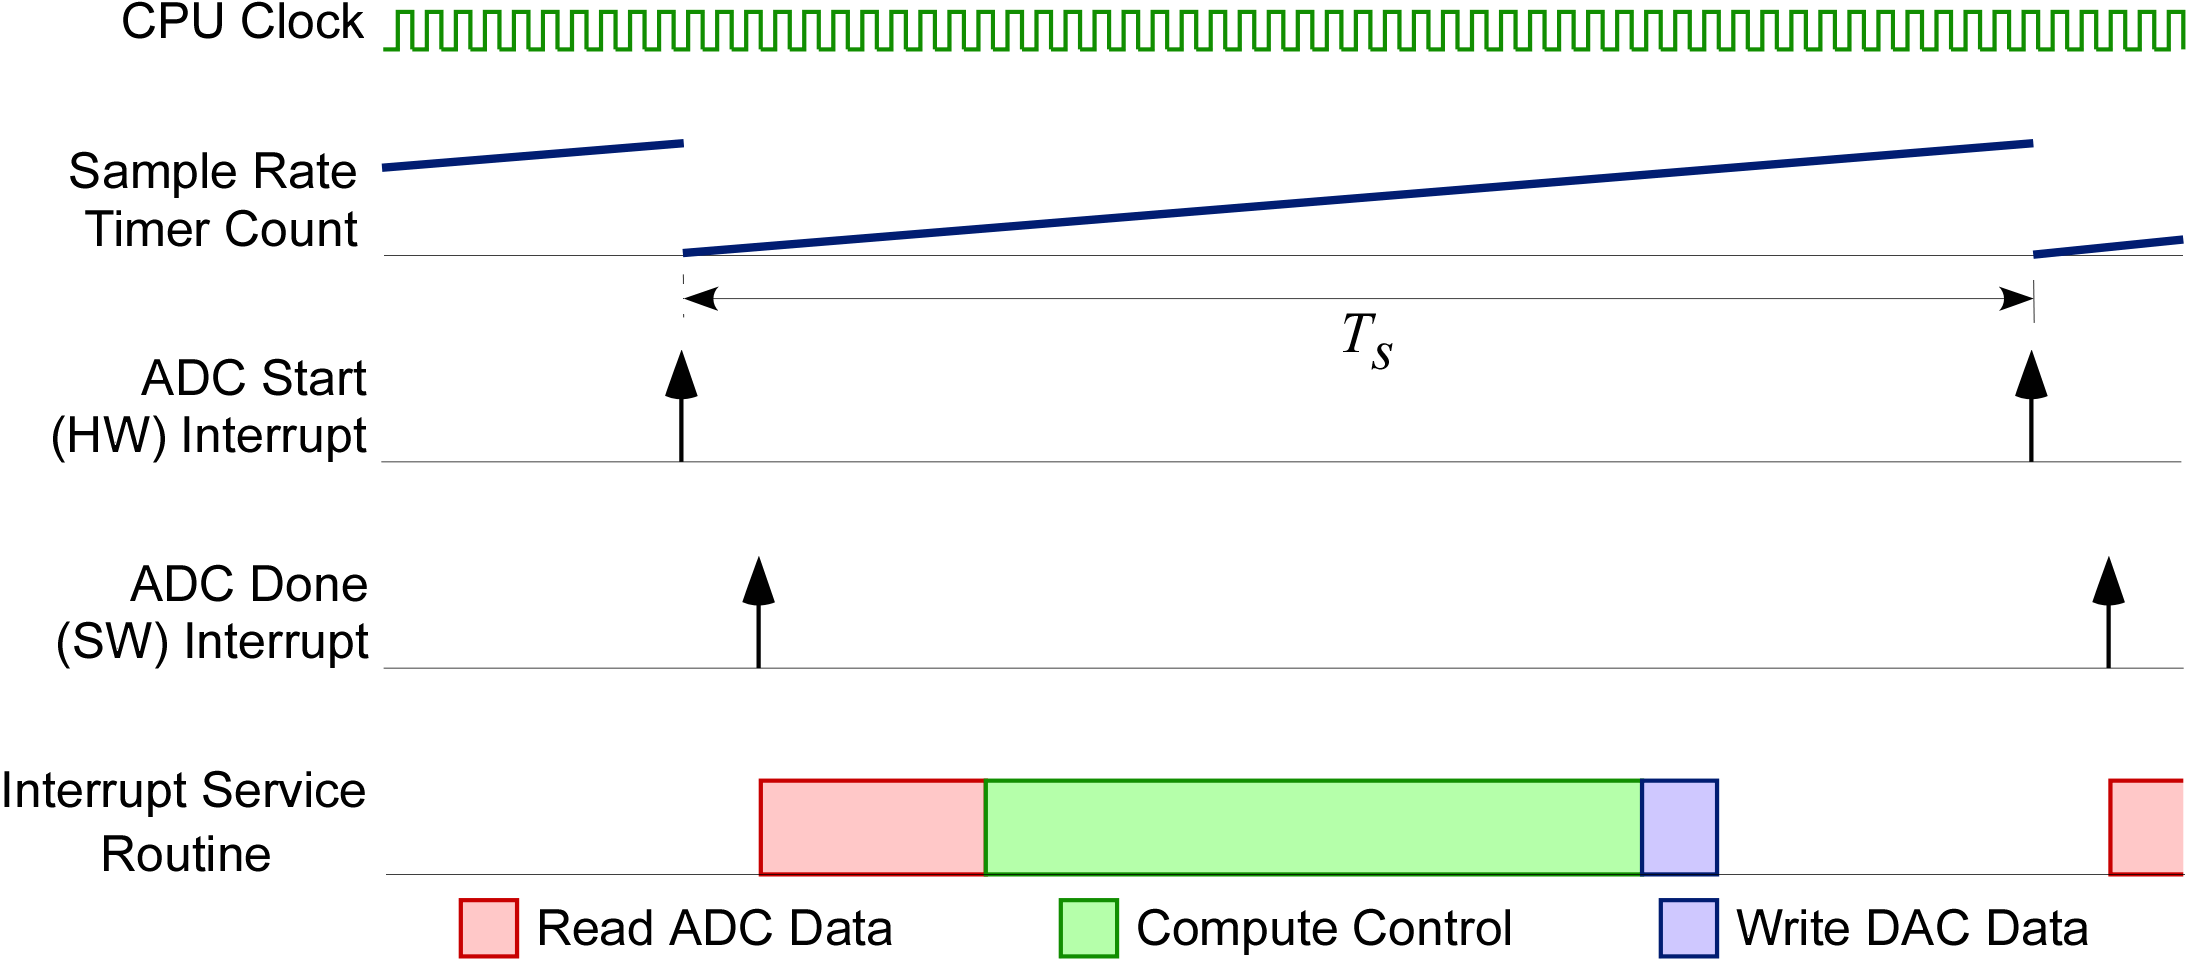
\includegraphics[width=\textwidth]{timing_diagram_large}
    \caption[Timing diagram of a real-time software loop of a \glsfmtshort{bms}]
    {Timing diagram of a real-time software loop of a \gls{bms}. The sequence of
        events within one sample period $T_s$ in relation to the base clock of
        the controller is shown. Particular emphasis is placed on depicting the
        handling of \gls{isr} requests pertinent to cell models. Other
        background tasks performed by the CPU is de-emphasised. Moreover, the
        integration of the  \gls{bms} software loop within  the larger  scope of
        a master  vehicular controller is not shown. Illustration adapted from
    Southward~\cite{Southward2011}.}
    \label{fig:timingdiagramBig}
\end{figure}

\Cref{fig:timingdiagramBig}   depicts   an   exploded   view   of   the   timing
aspects  of  the  \textsc{Interrupt  Service  Routine}  that  was  presented  in
\cref{subfig:fgRTprocess}.  Upon  the  expiry  of an  on-chip  timer  calibrated
against a  baseline precision-clock,  hardware interrupts are  raised by  one or
more \glspl{adc} associated  with voltage/current sensors mounted  on cells. The
\gls{isr}  disables  the interrupt  and  reads  the  samples  of data  from  the
\glspl{adc} into software. At the end  of this process, the \gls{isr} rearms the
interrupts  and  simultaneously sends  and  acknowledgement  to the  appropriate
sensor  which  reloads  its  timer.  The  \gls{spm}  model  equations  are  then
evaluated in software and resulting  computational variables such as voltage and
concentrations  is used  in other  activities such  as state  estimator. If  the
\gls{bms} also performs control tasks, \eg{}~regulating the coolant-flow rate or
\gls{ice} state-toggling such  as in the hysteresis control of  a series hybrid,
these control outputs are written to the relevant \glspl{dac}.


% \FloatBarrier

\subsection{Sample Delay Considerations}

\Cref{fig:timingdiagramSmall} shows a timeline view of all CPU activities across
a larger  time horizon.  The CPU's  load factor is  the ratio  of time  spent in
foreground requests to  its idling time. While a high  load factor is beneficial
in  terms of  efficient  usage  of resources,  it  adversely  affects the  power
efficiency of the chip.

\begin{figure}[!htbp]
    \centering
    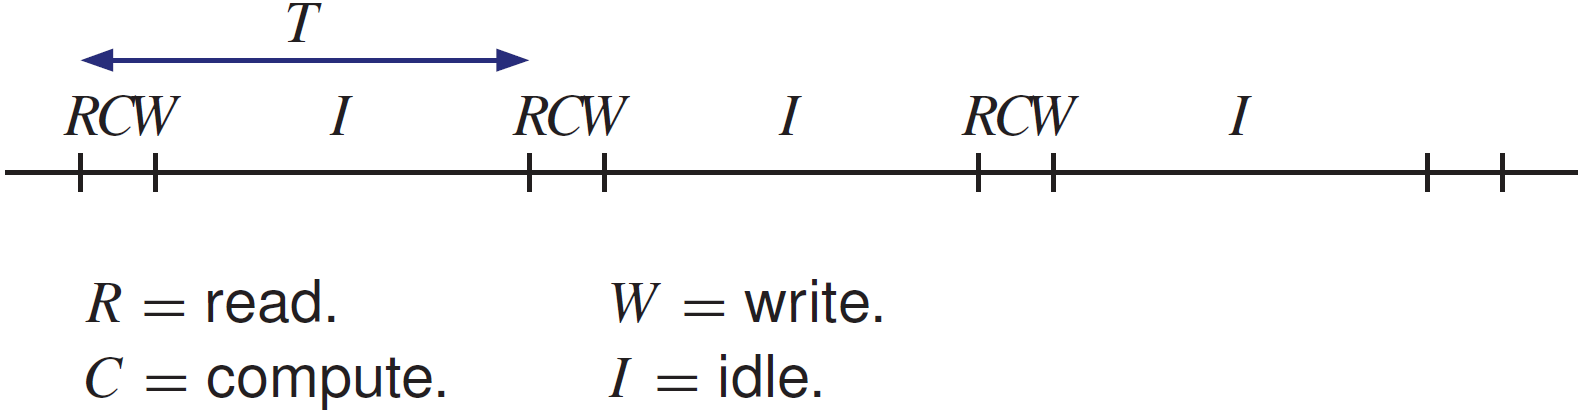
\includegraphics{timing_diagram_small}
    \caption[Timeline of \glsfmtshort{bms} activities over multiple CPU cycles of a real-time
    controller]{A compressed timeline of CPU execution cycles showing details of
        activities within each sample interval. The execution sequence is shown
        over a larger horizon so as to illustrate the proportion of `activity
        time' relative to the `idle time'. The vast majority of the CPU cycle is
        spent in idling or background tasks. The servicing of the \gls{isr}
        occupies a relatively small fraction of each CPU cycle. Diagram
    reproduced from Plett~\cite{PlettECE5540_02}.}
    \label{fig:timingdiagramSmall}
\end{figure}

For  Li-ion  cell  modelling,  a  sampling interval  of  $T_s  =  1$\si{\second}
is   commonly  used,   thus  aiming   to   capture  the   cell  dynamics   below
\SI{1}{\hertz}\footnote{In  the ideal  case, according  to the  Nyquist sampling
theorem.  In practice, the frequency  range is smaller.}. The CPUs clock is
several \si{\MHz}, a vast  majority of which is spent in  background tasks or in
sleep mode. Furthermore,  a low-latency \gls{isr} code is employed  in the tasks
of reading the  \gls{adc} value, evaluating the model equations  and writing any
control outputs to  the \gls{dac}. Using a simplified  physics-based models such
as the \gls{spm} helps in achieving a low-latency throughput for the \gls{isr}.

The overall implication of such a scheme  is that any \emph{delays} owing to the
sample and  hold process  at the model  input and outputs  can be  neglected. In
conventional sampled-data systems, control delays may be analysed by considering
a multiplicative factor of $e^{-sλ}$ in the Laplace domain transfer function of
the system.  Delay parameters of  $λ = 0.5  T_s$ or $λ  = 1 T_s$  are commonly
employed as conservative estimates. However, owing to the small CPU load factors
considered  as good  practice  in  concurrent programming,  this  delay term  is
omitted in this thesis for discrete-time formulation of the \gls{spm} model.


\subsection{Discrete-Time \glsfmtshort{spm} Formulation}

% \Cref{fig:blockdiagctsdisc} shows  a block  diagram representation of  the plant
% model its associated input and output signals.

Due  to the  sampling and  \gls{zoh} operations  at the  \gls{adc} input  to the
system,  the input  to the  \gls{spm} is  transformed from  a simple  continuous
time signal  to discrete-time  sequences \ie~\mbox{$u(t) \mapsto  u[k]$} and
\mbox{$y(t)  \mapsto  y[k]$}, where  \mbox{$k  =  0,1,\dots,∞$}~is the  sample
index  corresponding  to  the   continuous  time  instant~\mbox{$t_k  =  kT_s$}.
The  continuous  time  plant  model  represented  by  the  \gls{ode}  system  of
\cref{eq:threestatesmatrixvec} is therefore replaced  by a discrete-time process
and modelled by a \emph{difference} equation which is to be determined.

% \begin{figure}[!htbp]
%     \centering
%     % show block diagram cross-referencing equation and a question mark for the
%     % dt system
%     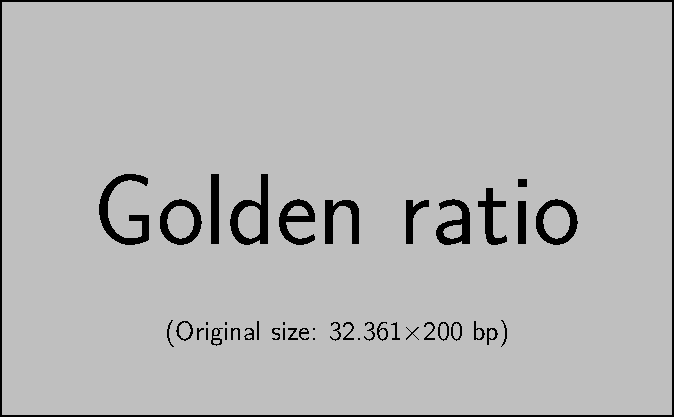
\includegraphics{placeholder_images/example-image-golden.pdf}
%     \caption[Block-diagram of continuous and discrete-time systems]{Block-diagram of the plant model and associated signals of a continuous-time system and its discrete-time counterpart}
%     \label{fig:blockdiagctsdisc}
% \end{figure}

Consider       the       general      continuous-time       solution       given
by \cref{eq:genanalyticctssoln}. Let $t_0 = k T_s$ and $t = (k+1)T_s$, where $k  =
0,1,\dots,∞$. Therefore,
\begin{alignat}{2}
    x(t_0) & = x(kT_s)     & & \equiv x[k] \\
    x(t)   & = x((k+1)T_s) & & \equiv x[k+1]
\end{alignat}
Substituting these relationships into \cref{eq:genanalyticctssoln},
\begin{equation}
    \mathbf{x}[k+1] = e^{A T_s}\mathbf{x}[k] + \int_{k T_s}^{(k+1)T_s}e^{A ((k+1)T_s-τ)}B \mathbf{u}(τ)\,dτ \label{eq:intermediatediscrete}
\end{equation}
With the  \gls{zoh} scheme  discussed here, $u(\tau)$  remains constant  from $k
T_s$ to $(k+1)T_s$,  and is equal to $u(kT_s)$ \ie~$u[k]$. Consider a change
of variable definition  for the dummy variable of integration  $\tau$ as $\eta =
(k+1)T_s -  \tau$. Thus,  $\tau = (k+1)T_s  - \eta$. Hence,  $d \tau  = -d\eta$.
Substituting these into \cref{eq:intermediatediscrete},
\begin{align}
    \mathbf{x}[k+1] &= e^{A T_s}\mathbf{x}[k] + \left[\int_{T_s}^{0}e^{A \eta }B \right] u[k]\,{-d\eta}\\
    \shortintertext{Reversing the order of integration leads to}
    \mathbf{x}[k+1] &= e^{A T_s}\mathbf{x}[k] + \left[\int_{0}^{T_s}e^{A \eta }B \,{d\eta} \right] u[k] \label{eq:disctimefulleqn}
\end{align}

\Cref{eq:disctimefulleqn} represents a discrete-time state-space representation
of the dynamics of the system whose generic representation is given by the
difference equation
\begin{equation}\label{eq:discgenericLTI}
    \mathbf{x}[k+1] = A_d x[k] + B_d u[k]
\end{equation}
where $A_d = e^{A T_s}$ and $B_d = \int_{0}^{T_s}e^{A \eta}B
\,{d\eta}$.
If the continuous-time system matrix, $A$ is invertible, a closed form
expression for $B_d$ is obtained as
\begin{align}
    B_d &= A^{-1}(A_d - I_n)B && \text{(if $A^{-1}$ exists)}
\end{align}
For the continuous time system matrix $A$ of the \gls{spm}, its determinant is
zero \ie~
\begin{equation}
\begin{vsmallmatrix}
    -30\frac{D_\spos}{R_\ppos^2} & 0                            & 0 \\
    0                            & -30\frac{D_\sneg}{R_\pneg^2} & 0 \\
    0                            & 0                            & 0
\end{vsmallmatrix} = 0
\end{equation}
and hence  is not invertible.  This necessitates  an explicit evaluation  of the
integral in \cref{eq:disctimefulleqn} for computation of the discrete-time input
matrix, $B_d$.

Since the only non-zero entries of the matrix lie along its main diagonal \ie~
its modes  are decoupled, the  matrix exponential  reduces to a  diagonal matrix
whose elements are simply the scalar exponentials of the original entries.
\begin{gather}
    A_d = e^{A T_s} = \exp\left(
        \begin{bmatrix}
            -30\frac{D_\spos}{R_\ppos^2} & 0                            & 0 \\
            0                            & -30\frac{D_\sneg}{R_\pneg^2} & 0 \\
            0                            & 0                            & 0
    \end{bmatrix} T_s \right)
    % \end{equation}
    % \begin{equation}\label{eq:A_d}
    % A_d
    =
    \begin{bmatrix}
        e^{-30\frac{D_\spos}{R_\ppos^2} T_s} & 0                                    & 0 \\
        0                                    & e^{-30\frac{D_\sneg}{R_\pneg^2} T_s} & 0 \\
        0                                    & 0                                    & 1
    \end{bmatrix} \label{eq:A_dinit} \\
    % \end{equation}
    % \begin{equation}
    B_d = \int_{0}^{T_s}e^{A \eta}B \,{d\eta}
    % \end{equation}
    % \begin{equation}\label{eq:B_dintermediate}
    % B_d
    =\bigint_{0}^{T_s} \left( \begin{bmatrix}
            e^{-30\frac{D_\spos}{R_\ppos^2} \eta} & 0                                    & 0 \\
            0                                    & e^{-30\frac{D_\sneg}{R_\pneg^2} \eta} & 0 \\
            0                                    & 0                                    & 1
        \end{bmatrix}\cdot
        \begin{bmatrix}
            \frac{45}{2} \frac{\hphantom{-}1}{R_\ppos^2 A \, l_\text{pos} a_\spos F} \\
            \frac{45}{2} \frac{-1}{R_\pneg^2 A \, l_\text{neg} a_\sneg F} \\
            \hphantom{\frac{45}{2}} \frac{-3}{R_\pneg  A \, l_\text{neg} a_\sneg F}
    \end{bmatrix} \right) \, d\eta \label{eq:B_dinit} \\
% \end{gather}
% \begin{equation}
    B_d = \begin{bmatrix}
        \hphantom{-}\frac{3}{4} \frac{1 - \exp\left(-30\frac{D_\spos}{R_\ppos^2}\right)T_s}{D_\spos A \, l_\text{pos} a_\spos F} \\[1em]
        -\frac{3}{4} \frac{1 -
        \exp\left(-30\frac{D_\sneg}{R_\pneg^2}\right)T_s}{D_\sneg A \, l_\text{neg} a_\sneg F} \\[1em]
        \hphantom{-}\hphantom{\frac{3}{4}} \frac{-3 T_s}{R_\pneg  A \, l_\text{neg} a_\sneg F}
    \end{bmatrix} \label{eq:B_d}
\end{gather}

The  discrete-time  matrix-vector  system  presented  in  \cref{eq:A_dinit}  and
\cref{eq:B_d} have  not been presented in  existing literature, but is  vital to
understanding  the  implementation  of  the \gls{spm}  in  digital  controllers.
Although, simpler  alternatives such as  Forward Euler methods are  available to
approximate the time-derivative  of the state vector, they  suffer from problems
such as increasing  rate of local truncation error  per time-step, necessitating
the use of  very high sample rates,  which increases the burden  on the embedded
controller. The matrix exponential approach is superior in terms of accuracy and
stability across a wide range of sample rates.

For a pre-determined sample-rate, the matrix exponential and hence the $A_d$ and
$B_d$  matrices  can be  computed  offline  on a  desktop  and  stored into  the
non-volatile storage  of the embedded  controller to  be loaded onto  RAM during
operation. The vectorised implementation of the state dynamics presented here is
highly  efficient  and  directly  amenable for  use  in  classical  state-vector
algorithms. For the cell's terminal voltage computation, the basic structure and
form  of the  output  equation given  by \cref{eq:spmoutputeqn} remains  intact,
except  that the  continuous time  variables $\left(\mathbf{x}(t),  u(t)\right)$
need to  be replaced  by their discrete-time  counterparts in  the corresponding
equation  set \crefrange{eq:spmbasicoutputvoltagefinal}{eq:csurfnegfromcavgneg}.
The discrete-time output  function $h_d$ is evaluated  \emph{after} updating the
state vector through \cref{eq:discgenericLTI}.
\begin{equation}\label{eq:discspmoutputeqn}
    y[k+1] = h_d(\mathbf{x}[k+1],u[k+1])
\end{equation}

The complete  sequence of steps  to implement  the discrete-time variant  of the
\gls{spm}  is given  in \cref{alg:disctimespm}. In  particular, it  can be  seen
that  the discrete-time  system  and  input matrices,  $A_d$  and  $B_d$ can  be
pre-computed  from the  parameter set  (refer to  line~\ref{algLine:computeAdBd}
in \cref{alg:disctimespm}),   using   the   matrix  exponential   approach.   In
\textsc{MATLAB}, this  can be achieved  by passing  the arguments of  the matrix
exponential to  the \verb+expm+  command. The  vectorised implementation  of the
discrete-time state equation given in line~\ref{algLine:discstateEq} is a set of
efficient linear  algebra operations consisting of  simple matrix-vector product
and vector-addition routines.

% -*- root: ../main.tex -*-
%!TEX root = ../main.tex
% this file is called up by main.tex
% content in this file will be fed into the main document
% vim:nospell

\begin{algorithm}[!htbp]
    \caption{Discrete-time \glsfmtshort{spm}}\label{alg:disctimespm}
    \addtocontents{loa}{\vskip 6pt} % https://latex.org/forum/viewtopic.php?t=6218
    \begin{algorithmic}[1]
        \Require Load profile \Comment{\eg~a \texttt{csv} file of $t$ vs.\ C-rate}
        \Require \gls{spm} parameter set  \Comment{\eg~stored in a struct \texttt{params}}
        \Userdata $z[1], t_\text{f,user}$, $t_\text{f,condition}$, cell capacity $I_\text{1C}$, sample rate $T_s$ \Comment{$t_\text{f,condition} \in  \left\{\texttt{max}, \texttt{min}\right\}$}
        \Ensure  $z[1], V_\text{cell}[1]$ within limits \Comment{index $[k=1] \wedgeq \text{time } (t=0) $}
        \Procedure{Simulate\gls{spm}}{}%{$z[1],t_\text{f,desired},T_s,I_\text{1C},\texttt{params}$}
            \State {$t_\text{f,desired} =
                \begin{cases}
                   \max(t_\text{f,user},t_\text{f,profile}),
                        &\text{%\scriptsize
                    if $t_\text{f,condition}$ == \texttt{max};}\\
                    \min(t_\text{f,user},t_\text{f,profile}),
                    &\text{%\scriptsize
                otherwise.}
                \end{cases}$} \Comment{\parbox[t]{0.25\textwidth}{may terminate early due to cut-off violations}}
                    \FullComment{\scriptsize Flexible end time. Extrapolate last C-rate from profile until $t_\text{f,desired}$ if necessary.}
            \State $N_\text{max} \gets \ceil*{\frac{t_\text{f,desired}}{Ts}} + 1$ \Comment{max iterations assuming no cut-offs}
            \State Allocate storage of size $\mathbb{R}^{N_\text{max}\times 1}$ for each simulation variable
            \State Compute $\mean{c}_\sneg$[1] as per \cref{eq:csfluxinitialcondition}
            \State $I[1] \gets I_\text{1C} \times  \text{C-rate}[1], \quad \mathbf{x}[1] \gets \vect{0,0, \mean{c}_\sneg[1]}$ \Comment{ $\text{C-rate}[1]$ from profile}
            \State \ColorLine{Compute $A_d$ and $B_d$ \Comment{as per \cref{eq:A_dinit} and \cref{eq:B_d}}}\label{algLine:computeAdBd}
            \State $V_\text{cell}[1] \gets \textsc{ComputeCellVoltage}(\textbf{x}[1],I[1],\texttt{params})$ \Comment{from direct feedthrough}
            \For{$k \gets 2 : N_\text{max}$}
                \State $I[k] \gets $ interpolate from profile using \gls{zoh}
                \State \ColorLine{$x[k] \gets A_d x[k-1] + B_d u[k-1]$ \Comment{\cref{eq:discgenericLTI}}}\label{algLine:discstateEq}
                \State Compute $z[k]$ as per \cref{eq:soccomputation}
                \State $V_\text{cell} \gets \textsc{ComputeCellVoltage}(\textbf{x}[k],I[k],\texttt{param}) $
                \If {$z[k] \text{ or } V_\text{cell}[k]$ exceeded cut-off limits}
                    \State $k \gets k - 1$ \Comment{data from last  step is invalid}
                    \State \textit{break};
                \EndIf
            \EndFor
        \EndProcedure

        \OutputEqn{\textbf{x},I,\texttt{params}} \Comment{uses discrete-time variants of eqs \ie~at index $k$}
            \State Compute $c_\snegsurf$ as per \cref{eq:csurfnegfromcavgneg}
            \Comment{consider saturating \ie~$c_\snegmin \le c_\snegsurf \le
            c_\snegmax$}
            \State Compute $\mean{c}_\spos$ as per \cref{eq:csposbulkfromcsnegbulk}
            \State Compute $c_\spossurf$ as per \cref{eq:csurfposfromcavgpos}
            \State Compute $V_\text{cell}$ as per \cref{eq:spmbasicoutputvoltagefinal}
        \EndOutputEqn%
    \end{algorithmic}
\end{algorithm}


This  thesis takes  an  inclusive view  taking into  account  that some  battery
researchers whose  focus is on fundamental  aspects of lithium ion  cells, \eg{}
those specialising in  electrochemistry, might not be familiar  with the nuances
of  the  matrix exponential  and  discrete-time  matrix computations  (refer  to
line~\ref{algLine:computeAdBd} in \cref{alg:disctimespm}).  Therefore, a snippet
of \textsc{MATLAB} code  clarifying the computation of  the discrete-time system
and input matrices, $A_d$ and  $B_d$ is given in \cref{codesnippet:computeAdBd}.
A  full code  listing of  an example  discrete-time \gls{spm}  implementation in
\textsc{MATLAB} is provided in \cref{sc:disctimespm}.

\begin{listing}[!htbp]
\begin{minted}[mathescape,autogobble,bgcolor=mintedbg,escapeinside=||,texcomments=true]{matlab}
% Returns $A_d$ and $B_d$ matrices
A_cts = [-30*Ds_pos/(R_pos^2),                    0, 0; ...
                            0, -30*Ds_neg/(R_neg^2), 0; ...
                            0,                    0, 0];
% $A_d = e^{A T_s}$ \fontfamily{libertinus}\selectfont(see \cref{eq:A_dinit})
A_disc = expm(A_cts*Ts); % $\mathtt{expm}$ command computes the matrix exponential

B_cts = [ (45/2)/(R_pos^2*a_pos*L_pos*F*A); ...
         (-45/2)/(R_neg^2*a_neg*L_neg*F*A); ...
             (-3/(R_neg*a_neg*L_neg*F*A))];

% $B_d = \int_{0}^{T_s}e^{A \eta}B \,{d\eta}$ \fontfamily{libertinus}\selectfont(see \crefrange{eq:B_dinit}{eq:B_d})
B_disc = nan(size(B_cts));
B_disc(1) = B_cts(1)*(exp(A_cts(1,1)*Ts)-1)/A_cts(1,1);
B_disc(2) = B_cts(2)*(exp(A_cts(2,2)*Ts)-1)/A_cts(2,2);
B_disc(3) = B_cts(3)*Ts;
\end{minted}
\caption{Computation of discrete-time matrices $A_d$ and $B_d$ in
\textsc{MATLAB}}
\label{codesnippet:computeAdBd}
\end{listing}

Thus,  a  discrete-time model  of  the  basic  \gls{spm}  is now  available  for
implementation  in  an embedded  \gls{bms}.  Further  analysis of  discrete-time
issues  such  as  aliasing,  quantisation  noise,  signal  pre-conditioning  and
discrete fourier analysis  lies in the specialised engineering  domain of signal
processing and falls outside  the scope of the thesis. The  results of the basic
\gls{spm} are presented next in \cref{sec:basicspmsimresults}.

% \FloatBarrier

% % https://tex.stackexchange.com/questions/113719/cleveref-fails-to-reference-algorithms

% % https://tex.stackexchange.com/questions/110412/numbering-in-algorithmicx
% % https://tex.stackexchange.com/questions/65993/algorithm-numbering

% % https://tex.stackexchange.com/questions/203713/how-can-i-typeset-function-names-as-they-appear-in-algorithmic-environments
% % https://tex.stackexchange.com/questions/100346/typesetting-listofalgorithms-like-listoffigures-and-listoftables-using-titletoc
% % https://tex.stackexchange.com/questions/30363/how-do-i-define-a-new-command-in-algorithmicx

% % https://tex.stackexchange.com/questions/67908/customizing-the-algorithmic-package-break-and-loop-labels

% % https://tex.stackexchange.com/questions/69449/avoid-putting-statements-on-the-same-line-with-algorithmicx

% % \usepackage{float}
% % \newfloat{algorithm}{t}{lop}
% % Add \floatname{algorithm}{Algorithm} to capitalise the float name


\section{Desktop Simulation}\label{sec:basicspmsimresults}
% -*- root: ../../main.tex -*-
%!TEX root = ../../main.tex
% this file is called up by main.tex
% content in this file will be fed into the main document
% vim:textwidth=80 fo=cqt

In this  section, the performance  of the  basic \gls{spm} is  discussed through
desktop  simulation and  by comparison  against a  standard \gls{dfn}  benchmark
model incorporating the full \gls{p2d} dynamics.

% \footnote{In  this   thesis,  the  terms   \gls{p2d}  and  \gls{dfn}   are  used
% synonymously.  This   is  because,   although  the  \gls{dfn}   model  equations
% are  originally  derived  and  is  applicable  in  three  dimensions,  its  most
% common  implementation  is  the  pseudo-two dimensional  case  wherein  dynamics
% of  all  variables  other  than  solid concentration  are  evaluated  along  the
% through-thickness  direction of  the  cell (direction  of  the most  significant
% charge  transport). The  solid diffusion  equation  is computed  in a  spherical
% co-ordinate system on a separate pseudo-dimension  and is coupled with the axial
% co-ordinates through the boundary flux at the surface of each particle.}

\subsection[Cell   Parametrisation]{Cell   Parametrisation\protect\footnote{Some
contents    in   this    section   overlap    with   \cref{sec:p2daugmentations}
and      represents     a      joint     effort      with     \mbox{Ian      D.\
Campbell}.}}\label{subsec:spmp2dparametrisation}

% -*- root: ../../main.tex -*-
%!TEX root = ../../main.tex
% vim:nospell

\begin{table}[!htbp]
    \small
    \caption[Simulation parameters of  an \glsfmtshort{lco} cell]{Complete set of  parameters for  isothermal simulation of the
        \gls{p2d} and  \gls{spm} implementations  of an  \gls{lco} cell  (with \ch{LiCoO_2}--\ch{LiC_6} electrode   pair
        and   \ch{LiPF_6}   electrolyte).   The  highlighted   entries represent the  parameters exclusive  to \gls{p2d}
        model.\quad  \protect{$j \in \{\text{pos},\text{sep},\text{neg}\}$}}
    \label{tbl:lcoSimParamsSPMp2d}
    \vspace{-2.6229525pt}
    \begin{threeparttable}
        \centering
        \begin{varwidth}[t]{0.48\linewidth}
            \begin{tabular*}{\textwidth}{@{} l @{\extracolsep{\fill}} r @{}}
                \multicolumn{2}{c}{\textbf{System Conditions}} \\
                \toprule
                % \multicolumn{1}{@{}l}{Parameter} \\
                % \midrule

                Lower cutoff cell voltage, $V_\text{min}$ (\si{\volt}) & \tnote{a}2.50   \\
                Upper cutoff cell voltage, $V_\text{max}$ (\si{\volt}) & \tnote{b}4.30   \\

                \bottomrule
            \end{tabular*}
        \end{varwidth}
        \hfill
        \begin{varwidth}[t]{0.48\linewidth}
            \begin{tabular*}{\textwidth}{@{} l @{\extracolsep{\fill}} r @{}}
                \multicolumn{2}{c}{\textbf{Other Constants}} \\
                \toprule
                % \multicolumn{1}{@{}l}{Parameter} \\
                % \midrule

                Faraday constant, $F$ (\si{\coulomb\per\meter})                                                        & 96487         \\
                Universal gas constant, $R$ (\si{\joule\per\mole\per\kelvin})                                          & 8.314         \\

                \bottomrule
            \end{tabular*}
        \end{varwidth}

        \smallskip
        % \vspace{-2.6229525pt}
        % \vfill
        \begin{tabular*}{\textwidth}{@{} l @{\extracolsep{\fill}} r @{}}
            \multicolumn{2}{c}{\textbf{Cell-level Parameters}} \\
            \toprule
            % \multicolumn{1}{@{}l}{Parameter} \\
            % \midrule

            Cell temperature, $T_\text{cell}$ (\si{\kelvin})                                                               & \tnote{c}298.15      \\
            \textcolor{viridistwentybluesix}{\emph{Init.}}\ electrolyte conc., $c_\text{e,0}$ (\si{\mole\per\meter\cubed}) & \tnote{c}1000        \\
            Overall active surface area, $A$ (\si{\meter\squared})                                                         & \tnote{i}\num{2.053} \\

            \bottomrule
        \end{tabular*}

        \smallskip
        \begin{tabular*}{\textwidth}{@{} =P{7.5cm} @{\extracolsep{\fill}} +l +c +r @{}}
            \multicolumn{4}{c}{\textbf{Thermodynamic, Kinetic, Geometric and Transport Parameters}} \\
            \toprule
            \multicolumn{1}{@{}l}{Parameter} & \multicolumn{1}{l}{Pos} & \multicolumn{1}{c}{Sep} & \multicolumn{1}{r@{}}{Neg}\\
            \midrule

            \rowstyle{\color{viridistwentybluesix}} Bruggeman coefficient, $\text{brugg}_j$                                                 & \tnote{c}\num{4}        & \tnote{c}\num{4}                               & \tnote{c}\num{4}        \\
            \rowstyle{\color{viridistwentybluesix}} Intrinsic electrolyte diffusivity, $D$ (\si{\meter\squared\per\second})               & \tnote{d}\num{3.22e-10} & \tnote{d}\num{3.22e-10}                        & \tnote{d}\num{3.22e-10} \\
            \rowstyle{\color{viridistwentybluesix}} Intrinsic electrolyte conductivity, $\kappa$ (\si{\siemens\per\meter})                &
            \multicolumn{3}{c}{\textcolor{viridistwentybluesix}{\Vhrulefill{} see table note \emph{e} \& \cref{subsec:basicspmsimsetup} \Vhrulefill{}}}\\
            \rowstyle{\color{viridistwentybluesix}} \ch{Li^+} transference number, $t^0_\text{+}$                                           & \tnote{c}\num{0.363}    & \tnote{c}\num{0.363}                           & \tnote{c}\num{0.363}    \\
            \rowstyle{\color{viridistwentybluesix}} Intrinsic electronic conductivity, $\sigma_j$ (\si{\siemens\per\meter})                 & \tnote{c}\num{100.00}   & ---                                            & \tnote{c}\num{100.00}   \\
            Thickness, $l_j$ (\si{\meter})                                                          & \tnote{c}\num{72e-6}    & \textcolor{viridistwentybluesix}{\tnote{c}\num{25e-6}} & \tnote{f}\num{88e-6}    \\
            Electrolyte porosity, ${\varepsilon}_j$                                                 & \tnote{c}\num{0.385}    & \tnote{c}\num{0.724}                           & \tnote{c}\num{0.485}    \\
            Filler vol.\ fraction, ${\varepsilon}_{\text{fi}_j}$                                    & \tnote{c}\num{0.025}    & ---                                            & \tnote{c}\num{0.033}    \\
            Particle radius, $R_\pj$ (\si{\meter})                                                  & \tnote{c}\num{2e-6}     & ---                                            & \tnote{c}\num{2e-6}     \\
            Specific interfacial surface area, $a_\sj$ (\si{\meter\squared\per\meter\cubed})        & \tnote{g}\num{885e3}    & ---                                            & \tnote{g}\num{723.6e3}  \\
            Electrode diffusivity, $D_{\text{s}_j}$ (\si{\meter\squared\per\second})                & \tnote{c}\num{1e-14}    & ---                                            & \tnote{c}\num{3.9e-14}  \\
            Stoichiometry, 0\% SOC, ${\theta}_{\text{min}_j}$                                       & \tnote{h}\num{0.9917}   & ---                                            & \tnote{h}\num{0.0143}   \\
            Stoichiometry, 100\% SOC, ${\theta}_{\text{max}_j}$                                     & \tnote{c}\num{0.4955}   & ---                                            & \tnote{c}\num{0.8551}   \\
            Max concentration, ${c_\text{s,max}}_j$ (\si{\mole\per\meter\cubed})                    & \tnote{c}\num{51554}    & ---                                            & \tnote{c}\num{30555}    \\
            Reaction rate coefficient, $k_\jr$ (\si{\meter\tothe{2.5}\mole\tothe{-0.5}\per\second}) & \tnote{c}\num{2.33e-11} & ---                                            & \tnote{c}\num{5.03e-11} \\
            Open circuit potential, $U_j$ (\si{\volt})                                              & \tnote{k}see table note & ---                                            & \tnote{m}see table note \\
            \bottomrule
        \end{tabular*}

        \smallskip
        % \vspace{-2.6229525pt}
        % \vfill
        %%%%%%%%%%%%%%%%%%%%%%%%%%%% SIMULATION PARAMS TABLE %%%%%%%%%%%%%%%%%%%%%%%%%%%%%
        \begin{tabular*}{\textwidth}{@{} =P{7.5cm}  +l@{\extracolsep{\fill}}+c +r @{}}
            \multicolumn{4}{c}{\textbf{Spatial Discretisation}} \\
            \toprule
            \multicolumn{1}{@{}l}{Parameter} & \multicolumn{1}{l}{Pos} & \multicolumn{1}{c}{Sep} & \multicolumn{1}{r@{}}{Neg}\\
            \midrule

            \rowstyle{\color{viridistwentybluesix}} Nodes, through-thickness (axial), $N_{\text{a}_j}$          & \num{15} & \num{15} & \num{15} \\
            \rowstyle{\color{viridistwentybluesix}} Nodes, within spherical particle (radial), $N_{\text{r}_j}$ & \num{10} & ---      & \num{10} \\

            \bottomrule
        \end{tabular*}

        % \smallskip
        % \vspace{-2.6229525pt}
        % \vfill
        \begin{tablenotes}[para,flushleft]
            \begin{scriptsize}
            \item[a] Ref.~\cite{Northrop2011}
            \item[b] Set to $\approx $\SI{100}{\milli\volt} above the cell's \gls{ocp} at \SI{100}{\percent} cell \gls{soc}
            \item[c] Ref.~\cite{Subramanian2009}
            \item[d] Computed at $T_\text{cell} = \SI{298.15}{\kelvin}$ using coefficients from table \romanletter{2} in Ref.~\cite{Valoen2005}\\%\fxnote{cross-ref to actual equation}
            \item[e] Computed at $T_\text{cell} = \SI{298.15}{\kelvin}$ using coefficients from table \romanletter{3} in Ref.~\cite{Valoen2005} at $c_\text{e,0}= \SI{1000}{\mole\per\meter\cubed}$\\
            \item[f] Set up for capacity balance of electrodes such that $l_\text{neg} = 1.22 \times l_\text{pos}$ here (see \cref{sec:electroderatio})
            \item[g] Computed as per \cref{eq:specificsurfarea}\\
            \item[h] Obtained as residual stoichiometries after a C/\num{500} simulated discharge from \SI{100}{\percent} cell \gls{soc} to \SI{2.7}{V}
            \item[i] Chosen so that current density for the electrochemical layer is \SI{29.23}{\ampere\per\meter\squared} for \SI{60}{\ampere} applied current (see \cref{sec:surfareaperlayer})
            \end{scriptsize}
            \vspace{0.5ex}
        \item[k] $ \mathcal{U(\theta_\text{pos})} = \textstyle \frac{-4.656 + 88.669\theta_\text{pos}^2 - 401.119\theta_\text{pos}^4 + 342.909\theta_\text{pos}^6 - 462.471\theta_\text{pos}^8 + 433.434\theta_\text{pos}^{10}}{-1 + 18.933\theta_\text{pos}^2 - 79.532\theta_\text{pos}^4 + 37.311\theta_\text{pos}^6 - 73.083\theta_\text{pos}^8 + 95.96\theta_\text{pos}^{10}}$ \hspace*{\fill}\refstepcounter{equation}(\theequation)\label{eq:lcoUocpPos}\\[0.25em]
            \begin{footnotesize}
            \item[m] $\mathcal{U(\theta_\text{neg})} = 0.7222 + 0.1387\theta_\text{neg} + 0.029\theta_\text{neg}^{0.5} - \frac{0.0172}{\theta_\text{neg}} + \frac{0.0019}{\theta_\text{neg}^{1.5}} + 0.2808 e^{(0.9 - 15\theta_\text{neg})} - 0.7984 e^{(0.4465\theta_\text{neg} - 0.4108)}$\hspace*{\fill}\refstepcounter{equation}(\theequation)\label{eq:lcoUocpNeg}\vfill
            \end{footnotesize}
        \end{tablenotes}
    \end{threeparttable}
\end{table}


\Cref{tbl:lcoSimParamsSPMp2d} lists  the simulation  parameters of  an \gls{lco}
cell  whose positive  and negative  electrodes are  \ch{LiCoO_2} and  \ch{LiC_6}
respectively.  The  electrolyte in  this  system  consists of  \ch{LiPF_6}~salt
in  a   solution  of   \gls{ec}/\gls{dmc}/\gls{emc}  in   a  1:1:1~ratio.  The
standard  set  of  \gls{dfn}  parameters have  been  extensively  described  and
documented  in  literature.  The   detailed  characterisation  of  the  physical
properties  of  lithium-ion  cells  falls  outside the  scope  of  this  thesis.
Here,  the vast  majority of  electrochemical parameters  \viz~the  geometric,
thermodynamic, kinetic  and transport properties  of the cell have  been sourced
from  Subramanian~\etal{}~\cite{Subramanian2009}. The  significance  of each  of
the  parameters  in  the  context  of the  modelling  assumptions  discussed  in
\cref{subsec:basicspmassumptions} is examined.

The simulation parameters that are applicable exclusively to the \gls{p2d} model
are shown as  highlighted text in \cref{tbl:lcoSimParamsSPMp2d}. It  can be seen
that only a  subset of the isothermal \gls{dfn} model's  parameters are required
for the \gls{spm}. In particular, there is no requirement to estimate any of the
electrolyte-related  parameters  in  each  electrode  region.  Furthermore,  the
properties of the separator material which  are necessary in the \gls{dfn} model
are also  not considered in the  \gls{spm} computations. A brief  enumeration of
the additional  \gls{p2d}-specific parameters in the  context of parametrisation
requirements is provided here.

\begin{enumdescriptnum}[leftmargin=!,itemsep=1ex,labelwidth=\widthof{$\symbf{\text{brugg}_j}\ \scriptstyle (\times 3)$abc}
    ,partopsep=0pt
    ,topsep=0pt
    ]

    \customenum{\text{brugg}_j}{3}  The  empirical Bruggeman  coefficient  helps
    to   define   the  effective   values   of   conductivity  and   diffusivity
    of   the  electrolyte.   Although  an   identical  value~(4)   is  used   in
    \cref{tbl:lcoSimParamsSPMp2d},  in  principle  all three  regions  can  have
    different values of brugg and need to be parametrised separately.

    \customenum{D}{1}  The  intrinsic  electrolyte   diffusivity  of  a  typical
    electrolyte  consisting  of  \ch{LiPF_6}~salt in  an  organic  solvent  was
    experimentally  characterised   and  provided  as  a   table  of  polynomial
    coefficients  by  Valøen  and  Reimers~\cite{Valoen2005}.  Evaluating  this
    polynomial  at a  cell  temperature of  \SI{298.15}{\kelvin}  results in  an
    intrinsic  diffusivity  of~\SI{3.22e-10}{\meter\squared\per\second}.  Since
    this is  a material property independent  of the region within  the cell, it
    needs to be parametrised only once.

    \customenum{\scalebox{1.35}{$\kappa$}}{1}   Like    the   diffusivity,   the
    intrinsic electrolyte conductivity is also a material property and its value
    is independent  of the region within  the cell. Unlike the  diffusivity, the
    electrolyte conductivity  is a strong  function of its  ionic concentration.
    Thus, the polynomial proposed by Valøen and Reimers~\cite{Valoen2005} needs
    to  be evaluated  at~$T_\text{cell}= \SI{298.15}{\kelvin}$  and  has to  be
    updated during the  simulation as salt concentration  within the electrolyte
    changes over time. A discussion on the choice of initial concentration is
    provided in \cref{subsec:basicspmsimsetup}.

    \customenum{\scalebox{1.25}{$t$}_+^0}{1}  The  cationic transference  number
    measures the relative  mobility of the \ch{Li^+}~ion in  the organic solvent
    and is  independent of  the region  within the  cell. Hence,  this intrinsic
    property is to be parametrised only once (per solvent).

    \customenum{\scalebox{1.25}{$\sigma$}_j}{2}  The  intrinsic conductivity  of
    the  solid phase  depends on  the material  used in  the porous  electrodes.
    Although a simplified  assumption of equal conductivity is used  for the two
    electrodes, in practice, this property needs to be characterised for each of
    the two electrodes.

\end{enumdescriptnum}

\sisetup{detect-weight=true}  Neglecting  Arrhenius-type temperature  dependence
of  physical  properties  and   their  corresponding  activation  energies,  the
basic  \gls{spm}  facilitates  the  ability to  afford  physics-based  modelling
capabilities with  \emph{eight} fewer parameters than  the equivalent isothermal
\gls{p2d} model. With  the naive assumption of equal  parametrisation effort per
physical property, this  implies a \textbf{\SI{20}{\textbf{\percent}}} reduction
in  parametrisation  requirements  for  the basic  \gls{spm}  when  compared  to
its  \gls{dfn} counterpart.  However,  considering the  fact that  parametrising
the  electrolyte's transport  properties requires  apparatus and  infrastructure
typically  available only  in specialised  chemical/materials~science labs,  the
reduction in parametrisation overhead  for system-level engineering stakeholders
is more pronounced.

Prima~facie, it may seem that electrolyte porosities and filler volume fractions
do  not  influence the  \gls{spm}  model.  However,  they  do have  an  indirect
bearing  on  arriving  at  a  critical parameter  \viz~the  solid  phase  volume
fraction~$\varepsilon_\sj$. This  parameter is required to  compute the specific
interfacial surface  area of the electrodes~$a_\sj$  \ie~the effective electrode
area  exposed to  reaction and  is an  important entity  in the  \gls{spm} model
equations  presented  in  \cref{subsec:basicspmgoverningeqns}. The  solid  phase
volume fractions  are also required in  simulating the \gls{p2d} model  owing to
the need for computing the effective electronic conductivities of the electrodes
(see \cref{eq:solidchargeconserve}). They are calculated as
\begin{equation}\label{eq:volumefraccalc}
    \varepsilon_\sj = 1 - \varepsilon_j - \varepsilon_{\text{fi}_j}
\end{equation}
where~$\varepsilon_j$  and~$\varepsilon_{\text{fi}_j}$  are the  electrolyte and
filler  volume-fraction  within  the  respective electrode  regions.  Using  the
values from \cref{tbl:lcoSimParamsSPMp2d} results in~${\varepsilon_\spos =
0.590}$
and  ${\varepsilon_\sneg  =  0.482}$~for the  positive  and  negative  electrodes
respectively. The specific interfacial surface areas are then calculated as
\begin{equation}\label{eq:specificsurfarea}
    a_\sj = \varepsilon_\sj \frac{4 \pi R_\pj^2}{\frac{4}{3} \pi R_\pj^3} = \frac{3\varepsilon_\sj}{R_\pj}
\end{equation}

As   discussed  in   the   assumptions  made   during   model  derivation   (see
\cref{subsec:basicspmassumptions})  and   consistent  with  the   assumed  model
geometry,  the  parameters  not  covered  by  the  \gls{spm}  pertain  to  those
describing electrolyte dynamics and distribution  of electronic charge along the
axial  thickness  direction  of  the  cell. Properties  such  as  the  intrinsic
diffusivities and conductivities of the  electrolyte as well as the transference
number of  \ch{Li^+} in the  organic solvent  are thus completely  redundant for
\gls{spm}  simulation.  The  assumption  of uniform  charge  density  along  the
through-thickness length of each electrode implies that the intrinsic electronic
conductivities of the two electrodes do not play any role in the model dynamics.
The porosities and Bruggeman coefficients in \cref{tbl:lcoSimParamsSPMp2d} serve
as  modifying factors  of the  intrinsic conductivities  and diffusivities  (see
\cref{tbl:dfneqns})  leading to  an effective  value within  each region  of the
electrochemical  layer. Thus,  their relevance  is  also rendered  void for  the
basic  \gls{spm}  simulation.  The  thickness of  the  separator  material  only
plays  a role  in  electrolyte behaviour.  By the  model  geometry presented  in
\cref{subsec:basicspmgeometry}, this  parameter also falls outside  the scope of
the basic \gls{spm}.

The  thicknesses  of the  electrodes  are  optimised  for equal  loading  \ie~to
achieve   a  balance   in   their  individual   capacities   to  store   \ch{Li}~atoms.  The  thickness  of  the  positive  electrode  is  chosen  as  the  value
from~Subramanian~\etal{}~\cite{Subramanian2009}. The  thickness of  the negative
electrode region  is then  computed with  the goal of  equalising the  volume of
active material  in each electrode  for every  electrochemical layer in  a pouch
cell.
\begin{equation}\label{eq:basiccapacitybalance}
    A_{\text{elec}_\text{pos}}\varepsilon_\spos l_\text{pos} = A_{\text{elec}_\text{neg}}\varepsilon_\sneg l_\text{neg}
\end{equation}

In a  lithium-ion pouch cell, the  electrodes are designed such  that the layers
can be  overlaid on  top of  one another  and finally  encapsulated in  a pouch.
Geometrical considerations  then imply  that the  cross-sectional area  (or face
area) of the two electrodes must be  the same. However, due to the consideration
of  avoiding  plating  at  the  edges  due  to  microscopic  malformations,  the
design  is done  such as  to have  a small  overhang of  the negative  electrode
layer~${(<  \SI{2}{\milli\meter})}$  with  respect  to  the  positive  electrode
layer~\cite{Bond2017} (see \cref{fig:anodeoverhangpouchcell}). Nevertheless, the
active surface area is just the  common overlap area between the two electrodes,
and hence $A_\text{elec}$~is  equal to the cross-sectional area  of the positive
electrode.

Thus, \cref{eq:basiccapacitybalance} reduces to~${\frac{l_\text{neg}}{l_\text{pos}} =
\frac{\varepsilon_\text{pos}}{\varepsilon_\text{neg}} = 1.22}$,~yielding~${l_\text{neg} = \SI{72}{\micro\meter}}$.

At  first,  it may  be  surprising  to note  that  the  values of  the  particle
radius~$R_\pj$  used  in both  the  \gls{p2d}  and \gls{spm}  remain  identical.
However, it is  important to note that the \gls{p2d}  equations of the \gls{dfn}
model  are cast  in a  normalised form  \ie~already set  up to  account for  the
overall capacity of  the cell under consideration implicitly through  usage of a
current density (per  unit area) for its simulation.  Furthermore, this explains
why increasing the number of discretisation nodes does not increase the modelled
capacity, but instead merely serves to improve the simulation accuracy owing to
the enhanced spatial resolution.

The  overall  active  surface  area~${A  = n  A_\text{elec}}$  is  the  combined
cross-sectional area of  all layers ($n$~is the number  of electrochemical (pos,
sep,  neg)  triplets)  stacked  into  the pouch  cell.  In  both  the  \gls{p2d}
and  \gls{spm}  models,  this  parameter  serves  to  scale  the  external  load
current  down  to  the  current  density  experienced  by  each  electrochemical
layer.  A   value  of  \approx\SI{30}{\ampere\per\meter\squared}   was  reported
in  the  results  section  of  Subramanian~\etal{}~\cite{Subramanian2009}.  When
considering a  \SI{60}{\amphour} pouch cell with  \SI{10}{\milli\meter} exterior
thickness   and  using   the   parameters  reported   in~\cite{Subramanian2009},
this  results  in  a  cross-sectional area  of  \SI{2.053}{\meter\squared}  (see
\cref{sec:p2daugmentations}). Considering the  equalisation of capacity loading,
with the  newly chosen thickness  value of  the negative electrode,  the 1C-rate
capacity of the cell has been revised to~\SI{29.23}{\ampere\per\meter\squared}.

On  simulating  the \gls{p2d}  model  with  a  trickle bleeding  type  discharge
corresponding   to   a  current   of   C/500   and   logging  the   data   every
\SI{1}{\milli\second}, after reaching \SI{2.7}{\volt}\footnote{From manufacturer
datasheets  for \protect{\gls{lco}}  chemistries,  this value  is considered  to
correspond to~\SI{0}{\percent} \protect{\gls{soc}}.}, the remnant concentrations
in  the two  electrodes  were noted.  The  corresponding residual  stoichiometry
values are reported in \cref{tbl:lcoSimParamsSPMp2d}.

% and is  consistent with  typical values reported  in literature  for \gls{lco}
% chemistries.\fxnote{citation needed here.} This validation is important, since
% below certain  stoichiometry thresholds,  the spinel/olivine structure  of the
% electrodes can become unstable and collapse\fxnote{citation needed?}.

Since      only      isothermal      cell     behaviour      is      considered,
\cref{tbl:lcoSimParamsSPMp2d}    omits     the    activation     energies    for
the    various   diffusivities    and   conductivities    of   materials    (see
\cref{subsec:basicspmsimsetup}  for further  thermal  considerations). For  this
reason, \cref{tbl:lcoSimParamsSPMp2d} does not include other material properties
such as specific heats, and thermal conductivities. No properties of the current
collectors appear in  the isothermal model equations for both  the \gls{p2d} and
\gls{spm} models  and hence are  omitted. All other  electrochemical properties,
\viz~stoichiometries  at \SI{100}{\percent}  \gls{soc}, maximum  concentrations,
diffusivities, reaction  rate coefficients and  \gls{ocp} of the  two electrodes
remain invariant between the \gls{p2d} and \gls{spm} models.

\subsection{Simulation Setup}\label{subsec:basicspmsimsetup}

For  reproducibility of  results, it  is important  to discuss  the system-level
parameters influencing simulation setup.

The lower  cut-off voltage  of the  cell is chosen  to be~\SI{2.5}{\volt}. This
is  deliberately  kept  lower  than  the voltage  corresponding  to  the  cell's
\SI{0}{\percent}~\ie~\SI{2.7}{\volt}.  If set  above  \SI{2.7}{\volt}  even
at  infinitesimally small  discharge  currents, the  cell  would cut-off  before
achieving complete discharge. Choosing a value lower than \SI{2.7}{V} means that
the cell gets a chance to recover its terminal voltage, despite spikes in highly
dynamic  load  currents  that  might  bring the  voltage  below  this  threshold
momentarily. If a low-enough value is  not chosen, a system-level shutdown shall
be  initiated  despite possessing  the  ability  to  continue to  operate  after
recovery  of terminal  voltage.  In this  case, choosing  a  cut-off voltage  of
\SI{2.5}{\volt} does  not damage the cell  since checks are in  place to monitor
the  \gls{soc}  and trigger  cut-off  in  the  event  of charge  depletion  (see
\cref{alg:ctstimespm,alg:disctimespm}).  Northrop~\etal~\cite{Northrop2011}  use
this value, although no specific explanation is given for this choice.

The  upper   cut-off  voltage   of  the  cell   is  chosen   at  \SI{4.3}{\volt}
\ie~\approx\SI{100}{\milli\volt} higher  than  the  equilibrium \gls{ocp}  at~\SI{100}{\percent} \gls{soc}. There are several  reasons for this smaller margin
at the upper end of the voltage spectrum.
\begin{description}[leftmargin=!,labelwidth=\widthof{\bfseries low
    probabilities},itemsep=1ex]

\item[safety] li-ion  cells are less  tolerant to overcharging and  can pose
    fire hazards.

\item[degradation]  overcharging  li-ion  cells  can  lead  to  plating  and
    accelerate other degradation mechanisms.

\item[low  C-rates]  charging C-rates  are  typically  lower than  discharge
    C-rates.

\item[CCCV charging]  For on-board  chargers, taper charging  (such as  in a
    \gls{cccv} profile) is activated, which  ensures that charging current drops
    off  rapidly, leading  to a  lower overvoltage  towards the  upper \gls{soc}
    range.

\item[low probabilities] The only charging event when an electrified vehicle
    is in motion is during regenerative braking. The vehicular \gls{bms} manages
    the operating window such that the starting \gls{soc} is much lower than the
    overvoltage  that  could  be  caused due  to  braking.  Furthermore,  during
    operation, net discharge events  occur more frequently than regenerative
    braking events.

\end{description}

For  both the  \gls{p2d} model  and the  \gls{spm} model,  the cell  temperature
is   kept   constant   at   its   initial   value   of   \SI{25}{\degreeCelsius}
(\SI{298.15}{\kelvin}). This might imply to the reader that the operation of the
lithium ion cell is assumed to be isothermal. While this is not true in general,
for  the C-rates  considered  here  (<5C), typical  in  a \gls{bev}  application
particularly for the  short-duration transient loads studied, it  is certainly a
valid  zeroth  order  coarse  approximation of  the  cell's  thermal  condition.
Detailed modelling of  thermal dynamics is not within the  scope of this thesis,
as  the primary  goal is  to  obtain a  \gls{pbm} incorporating  electrochemical
principles amenable for  embedded application. Hence, the  thermal dependence of
parameters through an Arrhenius-type relationship is also not considered. Future
work could  include performing  thermally coupled  simulations \ie~incorporating
thermally dependent parameters and  simplified heat generation expressions \eg~a
lumped thermal model could be employed  for both the \gls{spm} and \gls{p2d} and
their performances may be compared.

To  understand  the parametrisation  of  initial  concentration, the  expression
for   electrolyte  conductivity   needs  to   be  examined.   As  discussed   in
\cref{subsec:spmp2dparametrisation},  the intrinsic  conductivity of  a specific
type  of  electrolyte  is  a  material   property  that  depends  on  the  local
concentration of \ch{Li^+}~ions and temperature.  In the characterisation of the
electrolyte by  Valøen and  Reimers~\cite{Valoen2005}, the best  fit expression
for electrolyte conductivity was obtained as
\begin{multline}\label{eq:kappavsCeandT}
    \kappa_j(c_\text{e},T)(x,t) =  10^{-4} c_\text{e}(x,t) \bigl(-10.5 + \num{0.668e-3} c_\text{e}(x,t) + \num{0.494e-6}  c_\text{e}{(x,t)}^2\\
    + (0.074 - \num{1.78e-5}) c_\text{e}(x,t) - \num{8.86e-10} c_\text{e}{(x,t)}^2 \bigr)T(t)\\
	+ \left(\num{-6.96e-5} + \num{2.8e-8} c_\text{e}{(x,t)})T(t)^2\right)^2
\end{multline}

\begin{figure}[!htbp]
    \centering
    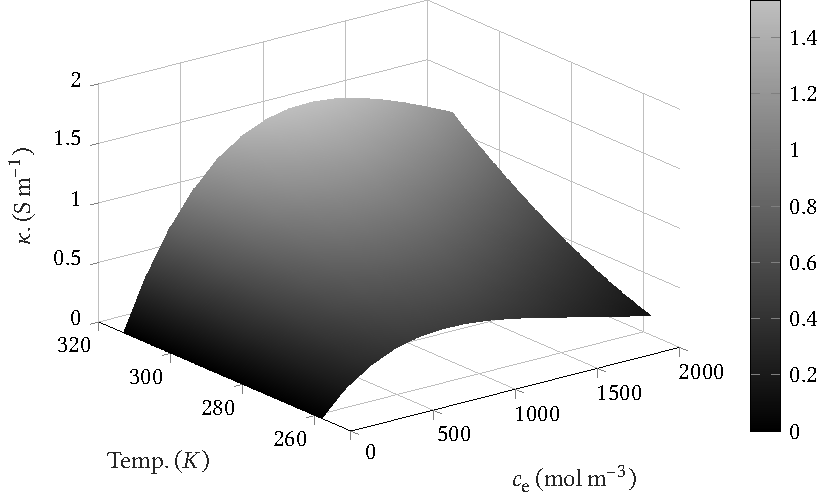
\includegraphics{m2t_kappa_ce_T.pdf}
    \caption[Surface plot of electrolyte conductivity]
    {Electrolyte conductivity as a function of cell temperature and initial concentration.
        % The variation of conductivity versus these factors is a smooth function.
    }%
    \label{fig:kappavsCeandT}
\end{figure}

\Cref{fig:kappavsCeandT}   shows    a   surface   plot   of    the   electrolyte
conductivity  as a  function  of initial  concentration~$c_\text{e,0}$ and  cell
temperature~$T_\text{cell}$. For the modelling task at hand, relevant aspects of
this  material property  can be  better understood  through the  simplifications
afforded by  the simulation conditions  applicable here. At  equilibrium initial
condition,  $c_\text{e}$~is uniform  over  the axial  space~$x$. Secondly,  only
isothermal  cell   behaviour  is   considered  \ie~${T(t)   =  T_\text{cell}(0)=
T_\text{cell}}$. Hence, \cref{eq:kappavsCeandT} reduces to
\begin{multline}\label{eq:kappavsCeinitandTcell}
    \kappa_j =  10^{-4} c_\text{e,0} \bigl(-10.5 + \num{0.668e-3} c_\text{e,0} + \num{0.494e-6}  c_\text{e,0}^2\\
        + (0.074 - \num{1.78e-5}) c_\text{e,0} - \num{8.86e-10}
    c_\text{e,0}^2 \bigr)T_\text{cell}\\
	+ \left(\num{-6.96e-5} + \num{2.8e-8} c_\text{e,0})T_\text{cell}^2\right)^2
\end{multline}

As inferred from \cref{fig:kappavsCeandT}, the electrolyte conductivity~$\kappa$
is    a    smooth    function    of~$c_\text{e}$    and~$T_\text{cell}$.    Thus
\cref{eq:kappavsCeinitandTcell}   can  be   effectively  visualised   through  a
parametric  plot of  $\kappa$ versus  $c_\text{e}$ with  $T_\text{cell}$ as  the
variable parameter  as seen in \cref{fig:kappavsce}.  From \cref{fig:kappavsce},
it  is  evident   that  at~${T_\text{cell}=\SI{298.15}{\kelvin}}$,  the  maximum
value   of    electrolyte   conductivity    is   attained    at~${c_\text{e}   =
\SI{1000}{\mole\per\meter\cubed}}$.  It  is  advantageous to  operate  the  cell
around  this   salt  concentration  so   as  to  minimise  the   cell's  overall
resistance.  Hence, the  initial  concentration~$c_\text{e,0}$ is  chosen to  be~\SI{1000}{\mole\per\meter\cubed}. It should be  noted that while the electrolyte
concentration  in  the  \gls{p2d}  model  exhibits  both  spatial  and  temporal
variations during  the simulation, in  the \gls{spm} model, it  remains constant
throughout.

\begin{figure}[!htbp]
    \centering
    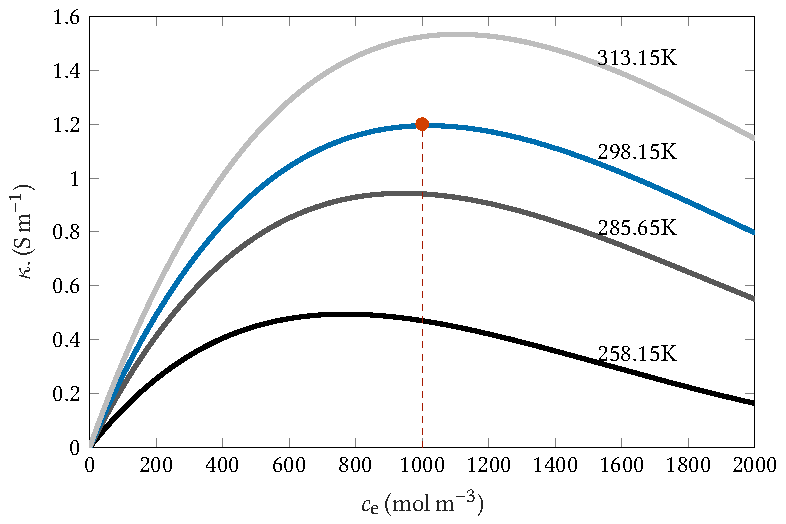
\includegraphics{m2t_kappa_ce_parametric_T.pdf}
    \caption[Electrolyte conductivity versus concentration at various cell
    temperatures]{Electrolyte conductivity versus equilibrium concentration at
        various cell temperatures. At~${T_\text{cell} = \SI{298.15}{\kelvin}}$,
        the maximum value of electrolyte conductivity corresponds to a salt
    concentration of~\SI{1000}{\mol\per\meter\cubed}.}
    \label{fig:kappavsce}
\end{figure}

The     reduction    in     parametrisation     requirements    discussed     in
\cref{subsec:spmp2dparametrisation}    is    only    one    of    the    factors
contributing  to  the  simplicity  and  ease  of  simulation.  As  discussed  in
\cref{subsec:basicspmgeometry}, an  important computational requirement  that is
present in the \gls{p2d} model, but  completely eliminated from the \gls{spm} is
the requirement of discretisation. As reported in \cref{tbl:lcoSimParamsSPMp2d},
with  15~nodes per  region  along the  axial direction  and  with 10~shells  per
electrode in the radial direction, the \gls{p2d} model under simulation achieves
mesh  independence  to  a  tolerance of~\approx\SI{2}{\percent}  for  the  range
of  C-rates  considered.  For  higher  C-rates,  coupling  a  thermal  model  is
of  higher  importance  than  incorporating  further  meshing  refinements.  The
discretisation-related parameters  are specific to  the \gls{p2d} model  and are
highlighted accordingly in \cref{tbl:lcoSimParamsSPMp2d}.

\subsubsection*{Capacity Characterisation}\label{subsubsec:capcharspmp2d}

First, it  must be  established that incorporating  the parameters  presented in
\cref{tbl:lcoSimParamsSPMp2d} into  the \gls{spm}  model equations results  in a
cell with  \emph{identical} capacity as the  \gls{dfn} model. This is  to ensure
the  validity  of  comparisons  in  further simulations.  Using  the  values  of
per-layer C-rate  as discussed  in \cref{subsec:spmp2dparametrisation},  and the
overall active  surface area from \cref{tbl:lcoSimParamsSPMp2d},  the cell under
simulation has a capacity of~\SI{60}{\amphour}.

Present literature  in battery modelling, both  for the \gls{dfn} model  and for
the  \gls{spm}, do  not  discuss  any aspect  of  capacity characterisation.  In
particular,  parameters  such  as  the  geometric  surface  area  of  cells  and
even  their 1C-rate  are often  not listed  in publications.  This practice  can
be  attributed  to  the  fact  that  all  one-dimensional  and  \glsfmtlong{p2d}
models operate  on a per-layer  basis, using an applied  current \emph{density}.
Many  a  time,  researchers assume  a  unit  surface  area  for the  cell.  This
implicit  normalisation  is amenable  to  those  studies  which strive  to  make
numerical comparisons  between models through  simulation. However, it  leads to
a  lack  of  clarity  on  the  actual capacity  of  the  cells  being  modelled.
Furthermore, when comparing with experimental data  from a real cell, such works
resort to  \mbox{ad hoc} techniques such  as empirical curve-fitting for  obtaining the
surface  area. Often  the  source of  such parametrisation  is  not made  clear.
\Cref{sec:p2daugmentations}  documents  the  details of  obtaining  the  overall
surface area  of cells  and arriving  at the  C-rate per  layer of  the specific
cell  under  consideration.  Since  the  \gls{dfn}  model  does  not  explicitly
model  the cell  capacity,  a brief  explanation  is provided  on  how a  simple
\emph{numerical}  characterisation can  be  used for  determining cell  capacity
given a \emph{complete} parameter list.

%\fxnote{citations needed for each accusation.}

For experimental capacity characterisation of cells, the standard practice is to
apply a very small discharge  current beginning at \SI{100}{\percent} \gls{soc},
logging the charge passed using a  high-precision coulomb counter until the cell
hits the voltage corresponding to \SI{0}{\percent} \gls{soc} as specified in the
manufacturer's datasheet. In order to decouple the effect of the cell's dynamics
from its  capacity, it is  required to  apply an infinitesimal  bleeding current
(tending towards, but not reaching \SI{0}{\ampere}).

Current sensors in battery cycler equipment use high-precision (typically 15--18
bit) \glspl{adc}  and are  able to  offer high  \glspl{snr} except  at ultra-low
currents. The main difficulty with using very low C-rates is that it drastically
slows down  the characterisation procedure.  Using a discharge  current of~C/100
\ie~\SI{0.6}{\ampere}  in  this case,  results  in  a characterisation  time  of
\SI{100}{\hour} or \mbox{\approx 4$\sfrac{1}{4}$}~days (excluding soak-times and
other set-up related activities).  Furthermore, for accurate coulomb-counting, a
high data logging  rate is needed, producing large file  sizes and corresponding
difficulties in post-processing them.  Considering moderate buffer-sizes used in
data logging modules of typical  cell-cycler software (shared between channels),
and  to  avoid  excessively  large wait-times  for  characterisation,  discharge
currents of C/20--C/25 are usually deemed sufficient.

In    order   to    validate    that   the    choice    of   model    parameters
result   in   an   intended   capacity  of   \SI{60}{\amphour},   an   analogous
procedure   is    carried   out   by    means   of   computer    simulation.   A
characterisation  simulation  beginning  at  \SI{100}{\percent}  \gls{soc}  with
a   discharge   current    of   \SI{0.6}{\ampere}   was   performed\footnote{All
computations  were  performed  on   a  64-bit  Hewlett-Packard~Z840  workstation
with   a   \mbox{16-core}   \mbox{\text{Intel}\textsuperscript{\textregistered}}
\mbox{Xeon\textsuperscript{\textregistered}}     \mbox{E5-2640~v3}     (Haswell)
processor clocked  at \SI{2.60}{\giga\hertz} with  \SI{128}{\giga\byte} DDR4~RAM
at 1866~MT/sec.}.  If the assumed  cell capacity  is indeed consistent  with the
model parameters,  then this corresponds to  a C-rate of~1/100.  Therefore, both
the \gls{p2d} and \gls{spm} should run  for exactly 100~hours before cut-off due
to charge depletion.


Capacity validation through computer simulation  is not bound by the limitations
of the experimental approach discussed earlier. Using 64-bit IEEE floating point
arithmetic,  quantities  as  low  as  ${\mathcal{O}(10^{-16})}$  can  be  safely
computed, nullifying  any \gls{snr} issues.  \Cref{tbl:charSimspmp2d} summarises
the key data  from this simulation run. For accurate  coulomb counting, the data
logging  interval is  set to~\SI{50}{\milli\second}.  Both models  ran close  to
100~hours.  The small  deviations from  this  expected termination  time can  be
attributed  to the  fact that  the  current is  not arbitrarily  small with  the
pragmatic goal of obtaining results in a reasonable time.

% -*- root: ../main.tex -*-
%!TEX root = ../main.tex
% this file is called up by main.tex
% content in this file will be fed into the main document
% vim:nospell

\begin{table}[!htbp]
    \centering
    \caption[Simulation data for capacity characterisation of \glsfmtshort{p2d} and \glsfmtshort{spm} models]{Simulation data for capacity characterisation of \glsfmtshort{p2d} and \glsfmtshort{spm} models. The \glsfmtshort{p2d} model is considered as the reference benchmark. The modelling error is defined as \protect{$\varepsilon_v = V_{\text{cell}_\text{p2d}} - V_{\text{cell}_\text{spm}}$}}
    \label{tbl:charSimspmp2d}
    \begin{tabular}{@{} l r r @{}}
        \toprule
        Parameter                                                               & Value  & Units              \\
        \midrule
        Data-logging interval                                                   & 50.00  & \si{\milli\second} \\
        Combined CPU time with warm cache                                       & 12.22  & \si{\minute}       \\
        Total RAM used                                                          & 603.90 & \si{\mega\byte}    \\
        \glsfmtshort{p2d} run-time                                              & 99.94  & \si{\hour}         \\
        \glsfmtshort{spm} run-time                                              & 99.90  & \si{\hour}         \\
        \glsfmtshort{p2d} discharge capacity                                    & 59.96  & \si{\amphour}      \\
        \glsfmtshort{spm} discharge capacity                                    & 59.94  & \si{\amphour}      \\
        Worst case error, $\varepsilon_{v_{\text{max}}}$                        & -94.30 & \si{\milli\volt}   \\
        Mean error, $\mu_{\varepsilon_v}$                                       & -3.00  & \si{\milli\volt}   \\
        \glsfmtshort{rms} error, $\varepsilon_{v_{\,\text{\glsfmtshort{rms}}}}$ & 8.20   & \si{\milli\volt}   \\
        \glsfmtshort{mae} error, $\varepsilon_{v_{\,\text{\glsfmtshort{mae}}}}$ & 3.20   & \si{\milli\volt}   \\
        Standard deviation of error, $\sigma_{\varepsilon_v}$                   & 7.60   & \si{\milli\volt}   \\
        \bottomrule
    \end{tabular}
\end{table}


As seen in \cref{tbl:charSimspmp2d}, even  the \emph{combined} \gls{cpu} time to
simulate both  the \gls{p2d}  and \gls{spm}  models is  two orders  of magnitude
lower than  real-time. The only  issue that remains to  be addressed is  that of
considerable memory and  storage requirements due to  high-rate data-logging for
accurate coulomb counting. For a standard computer workstation, this places only
a minor demand on its \gls{cpu}. For comparable volume of data to be logged, the
reliability  and ruggedness  of  a  dedicated workstation  far  exceeds that  of
real-time cell cyclers, thereby establishing numerical simulation as an amenable
method for characterisation of cell capacity. A major disadvantage of simulation
based capacity validation  is its extreme sensitivity to parameters  such as the
maximum concentration  of the  electrodes and  their stoichiometries,  which are
generally difficult to characterise. In this context, the experimental procedure
of  high-precision  coulomb counting  assumes  a  practical significance  as  it
requires no  knowledge of  the cell's parameters  other than  the manufacturer's
datasheet.


\Cref{fig:capcharspmp2d}  shows  the  voltage  response  of  the  \gls{spm}  and
\gls{p2d}  models,  which   overlap almost entirely.  It  is  clear  that   both  the  \gls{p2d}
and  \gls{spm}  models   achieve  a  run-time  of   100~hours.  This  represents
the   first  visualisation   of  results   produced  by   the  \gls{spm}   model
equations  discussed  in \cref{subsec:basicspmgoverningeqns} and  its  numerical
implementation  from \cref{sec:numericalimplementation}.

\begin{figure}[!htbp]
    \centering
    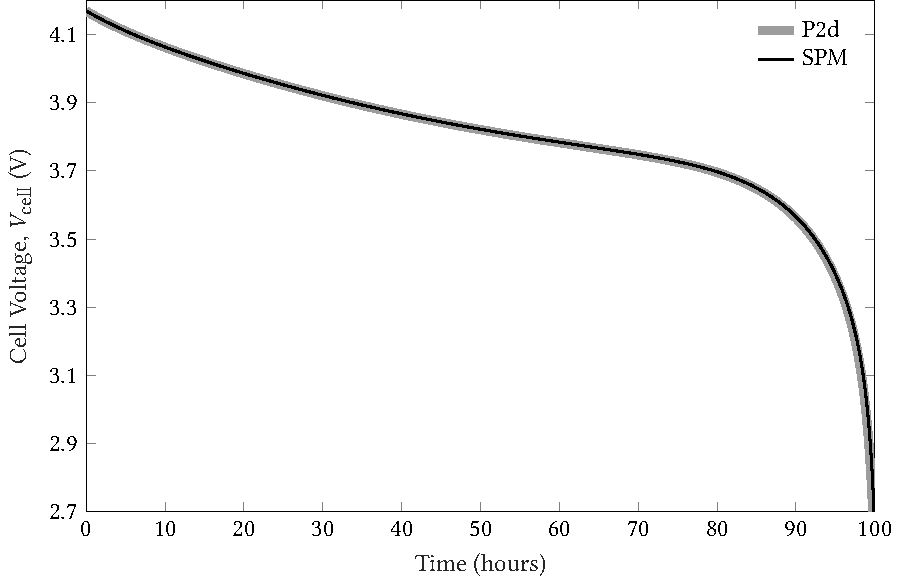
\includegraphics{capacity_match_spm_p2d.pdf}
    \caption[Voltage response of \glsfmtshort{spm} and \glsfmtshort{p2d} models
    for capacity validation]{Voltage response of \gls{p2d} and \gls{spm} models
        to a discharge current input of~\SI{0.6}{A}. Both models achieve their
        charge depletion point after \approx\SI{100}{\hour} confirming that
        their modelled capacities match. Key simulation data for this
    characterisation run is shown in \cref{tbl:charSimspmp2d}.}
    \label{fig:capcharspmp2d}
\end{figure}

The voltage  error  is defined as
\begin{equation}
    \varepsilon_v = V_{\text{cell}_\text{p2d}} - V_{\text{cell}_\text{spm}}
\end{equation}
The absolute maximum  error is of~$\mathcal{O}\left(100\right)\si{\milli\volt}$,
which  occurs  towards  the  end  of discharge.  Although  this  represents  the
worst  case upper  bound  on  the error,  this  is  not strictly  representative
of  the  overall  error  behaviour   as  evidenced  by  the  standard  deviation
of  the  error  vector.  The  mean   and  \gls{rms}  error  values  indicate  an
accuracy of~${\mathcal{O}\left(10\right)\si{\milli\volt}}$.  It should  be noted
that throughout  the simulation, the  voltage response of the  \gls{spm} remains
slightly above  that of  \gls{p2d}, thereby  leading  to a  negative value  for the  mean
voltage error. For continuous quantities  such as time-domain simulation outputs
of physical variables, the \gls{mae} is a suitable error metric and is
defined as
\begin{equation} \varepsilon_\text{\scriptsize  \glsfmtshort{mae}} =
\frac{\Sigma_{i=1}^{n}\abs{\varepsilon_i}}{n}
\end{equation}
Here, the numerical value of \gls{mae} is consistent with the order of magnitude
of the \gls{rms} and  mean error metrics as well as  with the standard deviation
of the error vector.

Thus,  a common  foundation  for  further simulations  has  been established  by
confirming  that  the  two  models  indeed  simulate  a  cell  with  a  capacity
of~\SI{60}{\amphour}.  With  the   cell  parametrisation  discussed,  simulation
setup  presented and  capacities  validated, the  simulation  results are  fully
reproducible and are presented next in \cref{subsec:simresultsbasicspm}.

\subsection{Simulation Results}\label{subsec:simresultsbasicspm}

\subsubsection*{Constant current discharge}\label{subsubsec:cnstcurrdischgsim}

The  left  column  of \cref{fig:cnstdischgspmp2dvoltage} shows  the  time-domain
voltage response of the basic \gls{spm} for various constant discharge currents.
The voltage response of the \gls{p2d} model  is also overlaid on these plots and
is used  as a  reference benchmark  for comparisons.  It is  difficult to  use a
common  time-scale for  the horizontal  axes of  the plots  since the  run-times
differ by two orders of magnitude for the C-rates considered.

\begin{figure}[!htb]
    \centering
    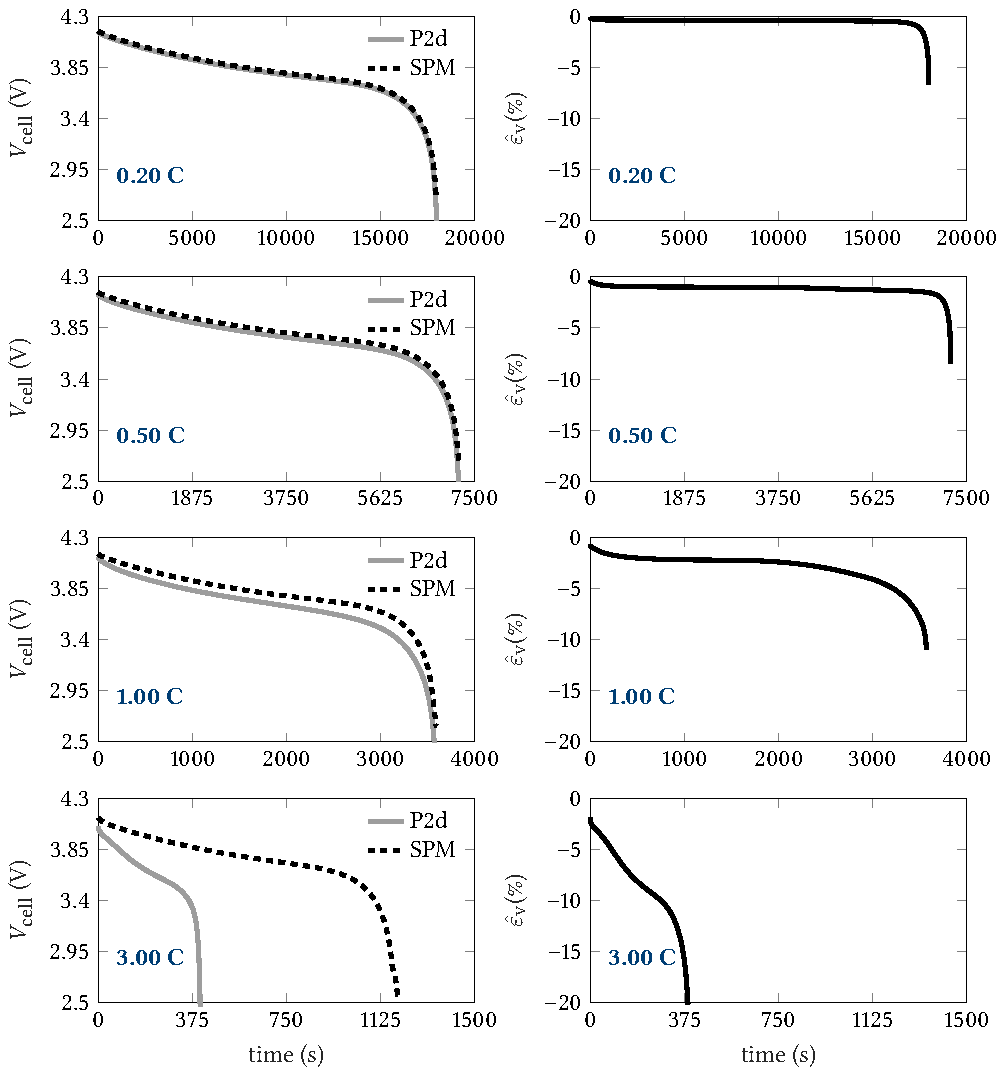
\includegraphics[width=\textwidth]{const_curr_dischg_voltage.pdf}
    \caption[Voltage responses of \glsfmtshort{p2d} and \glsfmtshort{spm} to
    constant current discharge]{Voltage responses of the \glsfmtshort{p2d} and
        \glsfmtshort{spm} models to various constant discharge rates. The left
        column shows the time-domain voltage response of the \gls{spm}
        plotted against the benchmark \glsfmtshort{p2d} response. The column on the
        right shows the percentage voltage error of the \glsfmtshort{spm} with
        respect to the \glsfmtshort{p2d} model. The performance of the
        \glsfmtshort{spm} degrades considerably at discharge currents above just~0.5C.}
    \label{fig:cnstdischgspmp2dvoltage}
\end{figure}

Since these comparisons  have to be done across multiple  C-rates, each yielding
different magnitudes in voltage responses, it is helpful to use a relative error
metric such as the percentage error, defined as
\begin{equation}
    \hat{\varepsilon}_v\,(\si{\percent}) = 100\frac{V_{\text{cell}_\text{p2d}} - V_{\text{cell}_\text{spm}}}{V_{\text{cell}_\text{p2d}}}
\end{equation}

It is to be noted that, in all cases, the \gls{p2d} model terminates faster than
the \gls{spm} either due to hitting lower cut-offs of either terminal voltage or
\gls{soc} (see \cref{fig:cnstdischgspmp2dsoc}).  Consequently, the  error vector
is defined only for the common time-region before cut-off.

In  \cref{fig:cnstdischgspmp2dvoltage},  the  column  on  the  right  shows  the
percentage error  in the voltage response  of the \gls{spm} with  respect to the
\gls{p2d} model.  At very  low C-rates  below \approx0.5C,  the voltage-response
performance of the \gls{spm} is acceptable. However, the performance degradation
is rapid above this C-rate. It is clear that the error in the \gls{spm} response
is monotonic and unidirectional. This indicates  that the source of the error is
due  to  unmodelled dynamics.  In  particular,  as  discussed in  the  modelling
assumptions  of  \cref{subsec:basicspmassumptions},  the \gls{spm}  ignores  the
electrolyte  dynamics.  Thus,  the  overpotential  in  the  electrolyte  is  not
modelled, which  results in the terminal  voltage of the \gls{spm}  being always
higher than its \gls{p2d} counterpart.

\begin{figure}[!htb]
    \centering
    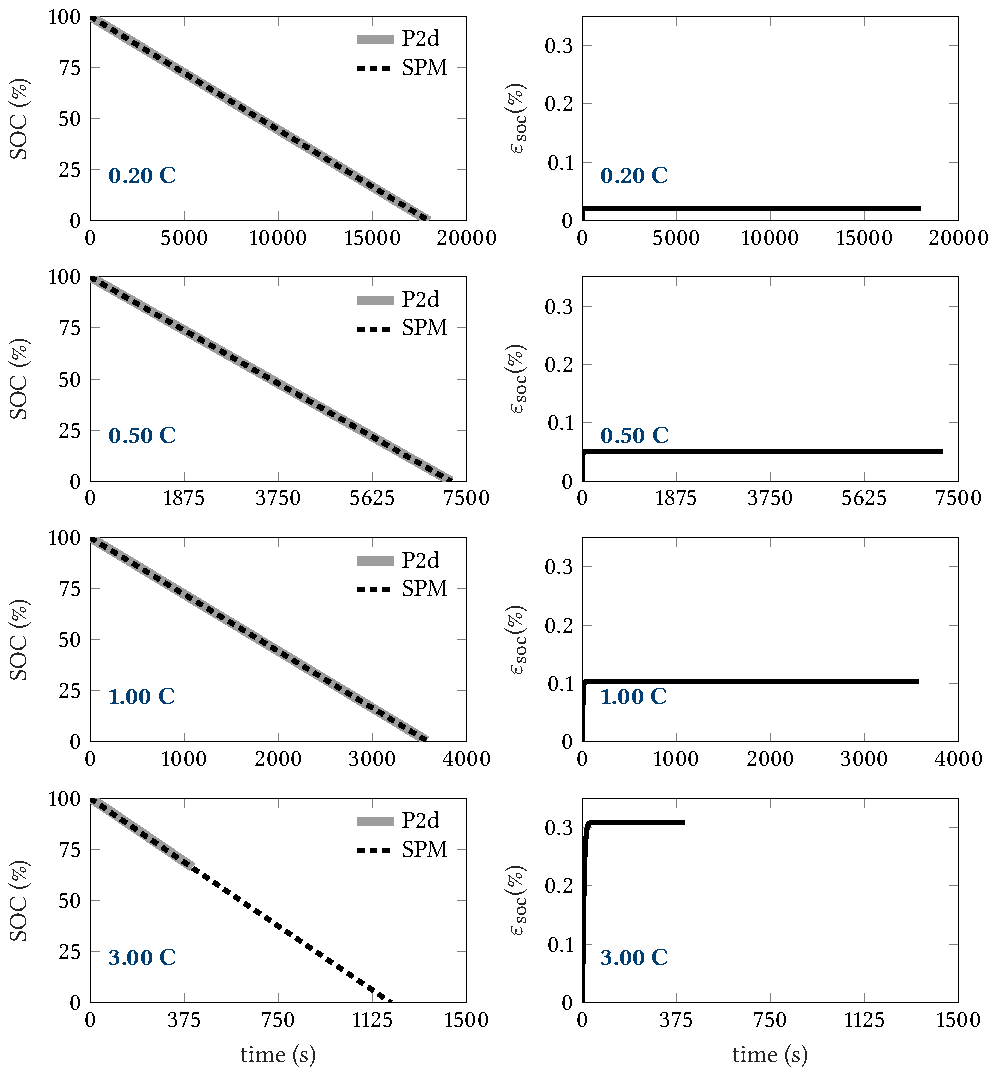
\includegraphics[width=\textwidth]{const_curr_dischg_soc.pdf}
    \caption[\glsfmtshort{soc} computed by \glsfmtshort{p2d} and
    \glsfmtshort{spm} models for constant current discharge]{Plots in the left
        column depict the time evolution of \glsfmtshort{soc} computed by the
        \glsfmtshort{p2d} and \glsfmtshort{spm} models for various constant
        discharge rates. The column on the right shows the error of the
        \glsfmtshort{soc} computed by the \glsfmtshort{spm} with respect to that
        computed by the \glsfmtshort{p2d} model \ie~$ \varepsilon_\text{soc}
        = {z_\text{p2d}} - z_\text{spm} $. The \glsfmtshort{spm} remains quite
    accurate even at moderate currents such as~3C.}
    \label{fig:cnstdischgspmp2dsoc}
\end{figure}

\Cref{fig:cnstdischgspmp2dsoc}  shows  the  time-evolution  of~\glsfmtshort{soc}
computed by the  \glsfmtshort{p2d} and the \glsfmtshort{spm}  models for various
discharge  currents. Since  the  \gls{soc} of  a cell  is  already a  normalised
quantity by  definition, the difference between  the two models can  be directly
used for comparison across C-rates. The \gls{soc} error is defined as
\begin{equation}
    \varepsilon_\text{soc} = {z_\text{p2d}} - z_\text{spm}
\end{equation}
and   like  the   error  in   the  terminal   voltage,  remains   unidirectional
over  time,   and  defined  only   until  one   of  the  models   hits  cut-off.
\Cref{tbl:errorsummarycntcurrdischgspmp2d}  shows  a  summary of  various  error
metrics used  to quantify  the performance  of the  basic \gls{spm}  for various
discharge rates.

% -*- root: ../../main.tex -*-
%!TEX root = ../../main.tex
% this file is called up by main.tex
% content in this file will be fed into the main document
% vim:nospell

\begin{table}[!htbp]
    \caption[Error-metrics summary of basic \glsfmtshort{spm} for constant current discharge]{Summary of error metrics
    of the basic \glsfmtshort{spm} for terminal voltage and \glsfmtshort{soc} in constant current discharge simulations.}
    \label{tbl:errorsummarycntcurrdischgspmp2d}
    \centering
    \begin{tabular}{@{} S S S S S @{}} \toprule
        {C-rate} & \multicolumn{2}{c}{$\hat{\varepsilon}_v\, (\si{\percent})$} & \multicolumn{2}{c}{$\varepsilon_\text{soc}\, (\si{\percent})$} \\
        \cmidrule(lr){2-3} \cmidrule(l){4-5}
        {}       & {abs.\ max.}                                                & \glsfmtshort{mae}                                               & {abs.\ max.} & \glsfmtshort{mae} \\ \midrule
        0.2      & 6.64                                                        & 0.49                                                            & 0.02        & 0.02        \\
        0.5      & 8.49                                                        & 1.17                                                            & 0.05        & 0.05        \\
        1.0      & 11.00                                                       & 2.95                                                            & 0.10        & 0.10        \\
        3.0      & 56.53                                                       & 9.22                                                            & 0.31        & 0.30        \\ \bottomrule
    \end{tabular}
\end{table}


A   quick   perusal  of \cref{tbl:errorsummarycntcurrdischgspmp2d}   reveals   a
discrepancy that invokes surprise at first glance. Whilst the performance of the
\gls{spm} is  quite poor in  terms of terminal  voltage prediction, it  is worth
noting that its \gls{soc} prediction  capabilities remain quite accurate even at
moderate  discharge  currents  of  about~3C and  therefore,  warrants  a  brief
explanation.

Referring to \cref{eq:soccomputation}, it is  seen that the \glsfmtshort{soc} of
the cell  is directly proportional  to the  bulk (average) concentration  in the
negative  electrode.  Hence  the plots  of  \cref{fig:cnstdischgspmp2dsoc}  also
represent the solid  phase concentration with a constant scaling  factor. As per
the assumptions listed in  \cref{subsec:basicspmassumptions}, the only transport
phenomena  modelled in  the \gls{spm}  is  solid phase  diffusion. However,  for
computation of the terminal  voltage, the electrolyte overpotential contribution
has  been  omitted  (see  \cref{eq:posoverpotential,eq:negoverpotential}).  This
explains  why  the  voltage  accuracy suffers,  while  the  open-loop  \gls{soc}
computation  remains  accurate.  The  high accuracy  of  \gls{soc}  (and  hence,
solid-phase  concentration)   computation  also  validates  the   usage  of  the
\engordnumber{4} order polynomial  approximation in the place of  Fick's law for
modelling solid-phase diffusion.

However,  the  discrepancy  in  accuracies of  terminal  voltage  and  \gls{soc}
computed  by the  basic \gls{spm}  leads to  an important  implication. Even  at
moderate C-rates, the  basic \gls{spm} \emph{cannot} be effectively  used in the
design of \gls{soc}  observers. This is because, the measured  voltage maps to a
vastly different  operating point when using  the \gls{spm} as the  plant model,
leading to strong deviations of the estimated \gls{soc}.


\subsubsection*{Constant current charge}\label{subsubsec:cnstcurrchgsim}

The \gls{cccv} charging  profile is a widely adopted  standard charging strategy
for charging lithium ion cells~\cite{Andrea2010}. In the constant current phase,
a charging rate of~1C is used  as an accepted baseline, although faster charging
strategies are presently being actively sought after.

% both in academia and in  particular, the automotive industry. For establishing
% the charging  performance of the basic  \gls{spm}, the standard rate  of~1C is
% used.

\begin{figure}[!htbp]
    \centering
    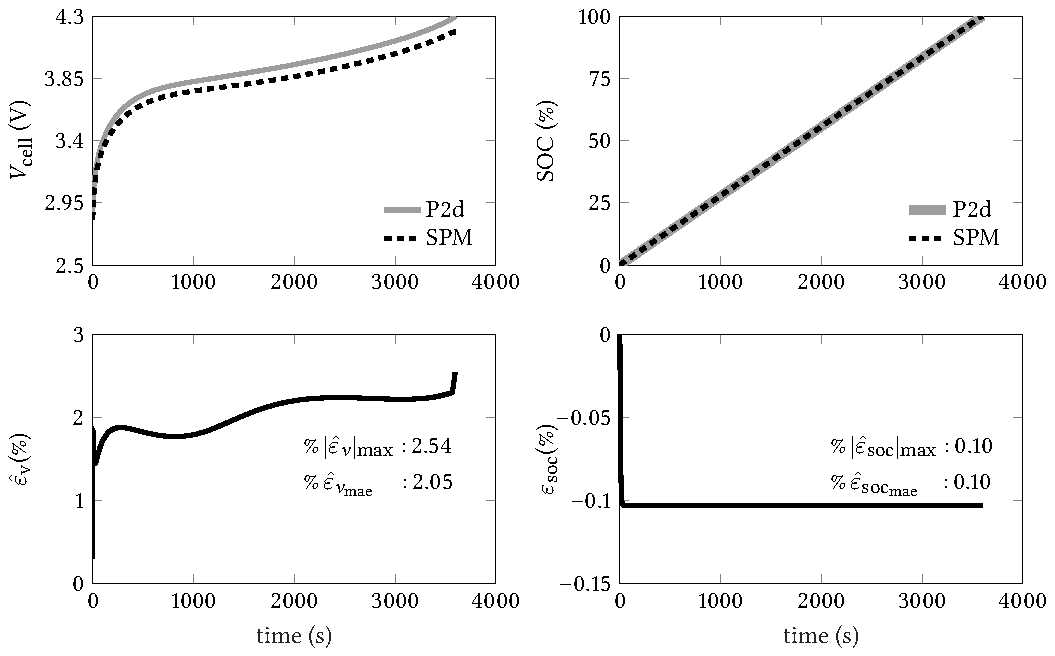
\includegraphics[width=\textwidth]{const_curr_chg.pdf}
    \caption[Voltage and \glsfmtshort{soc} computed by \glsfmtshort{p2d} and
    \glsfmtshort{spm} for 1C~constant current charge]{Time evolution of voltage
        and \glsfmtshort{soc} (top row) of the \glsfmtshort{p2d} and
        \glsfmtshort{spm} models upon charging with a constant current of~1C,
        \ie~\SI{60}{\ampere} starting at \SI{0}{\percent}~\glsfmtshort{soc}.
        The bottom row shows the percentage in terminal voltage and
        \glsfmtshort{soc} respectively of the \glsfmtshort{spm} with respect to
    the \glsfmtshort{p2d} model.}
    \label{fig:cnstchgspmp2d}
\end{figure}

The top row of \cref{fig:cnstchgspmp2d}  shows the evolution of terminal voltage
and \gls{soc}  of the \gls{p2d} and  \gls{spm} models under an  applied charging
current of~1C  \ie~\SI{60}{\ampere}. The constant-voltage charging  phase is not
shown. The bottom row shows the corresponding errors of the \gls{spm} model with
respect to  the reference  \gls{p2d} benchmark. The  corollary behaviour  of the
constant current discharge  behaviour is observed here. The  terminal voltage of
the \gls{spm}  remains below  the \gls{p2d} model  throughout. This  is expected
since, to  account for the  electrolyte voltage  drop modelled in  the \gls{p2d}
dynamics, a  higher terminal voltage needs  to be applied. The  voltage error is
thus  unidirectional and  remains positive  (opposite to  that observed  for the
corresponding  discharge  case). Similarly,  the  \gls{soc}  plots overlap  very
closely,  thereby validating  the underlying  polynomial approximation  of solid
phase diffusion.  It is  striking to  note that the  error in  \gls{soc} remains
exactly  around  the  same  magnitude (\approx\SI{0.1}{\percent})  in  both  the
charging and discharging cases.

\subsubsection*{Dynamic input profile}\label{subsubsec:dynamicspmp2dsim}

For automotive applications, it is  important to characterise the performance of
the  cell  model  under  dynamic load  conditions.  Several  standard  vehicular
driveycles  have been  defined and  adopted  by regulatory  agencies across  the
world.  These drivecycles  describe  the profile  of the  vehicle's  speed as  a
function of time.  The profile of speed versus time  of drivecycles is typically
available in intervals of \SI{1}{\second},  and is therefore consistent with the
sample interval used for the simulation (see \cref{tbl:lcoSimParamsSPMp2d}).

The \gls{udds} is  one such well-known drivecycle, originally  introduced by the
United  States  Environmental Protection  Agency  that  represents city  driving
conditions  which can  be  applied  to a  typical  mid-sized passenger  vehicle.
%  This  cycle  has  been  widely adopted  by  regulatory  agencies  across  the
world. \Cref{fig:uddsspeedvstimecycle}  shows the \gls{udds}  drivecycle wherein
the  vehicle's  speed  has  been  converted  to SI  units  for  use  in  further
computations.  One  complete  drivecycle runs  for~\SI{1369}{\second}.  As  seen
in  \cref{fig:uddsspeedvstimecycle}, the  \gls{udds} profile  is highly  dynamic
consisting  of  many sets  of  rapid  acceleration  and braking  events.  Hence,
this  drivecycle is  chosen to  provide  representative results  of the  model's
performance to dynamic inputs.

\begin{figure}[!htbp]
    \centering
    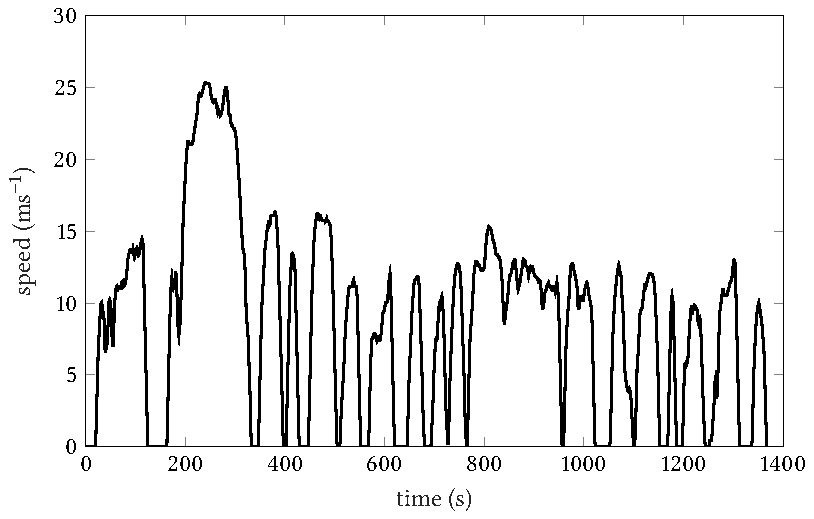
\includegraphics{udds_cycle.pdf}
    \caption{The \glsfmtshort{udds} drivecycle profile}
    \label{fig:uddsspeedvstimecycle}
\end{figure}

In  an  all-electric  drivetrain  wherein  lithium  ion  batteries  provide  the
propulsion power, the speed profile can be suitably converted to a corresponding
current  profile  experienced by  the  cell  through  the application  of  basic
governing   equations  from   vehicle   dynamics  (see   \cref{sec:accpathway}).
Therefore,  from  the  cell's  perspective, traversal  of  the  drivecycle  then
corresponds  to  the following  events.  During  acceleration phases,  the  cell
experiences  a  sharp  discharge  spike of  current.  Similarly,  assuming  that
regenerative  braking is  employed,  each deceleration  event  corresponds to  a
charging  current. Thus  a  current  versus time  dynamic  load  profile can  be
obtained. To  briefly summarise the  conversion process used here,  the computed
power profile of the cell is divided  by its nominal voltage and suitably scaled
so that the peak  of the current profile corresponds  to a discharge current
of~3C. Considering that all the braking energy cannot be recovered due to losses
at  the wheels,  brake discs  and  other mechanical  components, a  regenerative
braking  factor of  \SI{85}{\percent}  (the fraction  of  recoverable power)  is
assumed for  the charging scenario.

% The details  of this conversion for  a specific \gls{bev} platform  is discussed
% in~?\fxnote{fix this to point to layer opt chapter}.

\begin{figure}[!htbp]
    \centering
    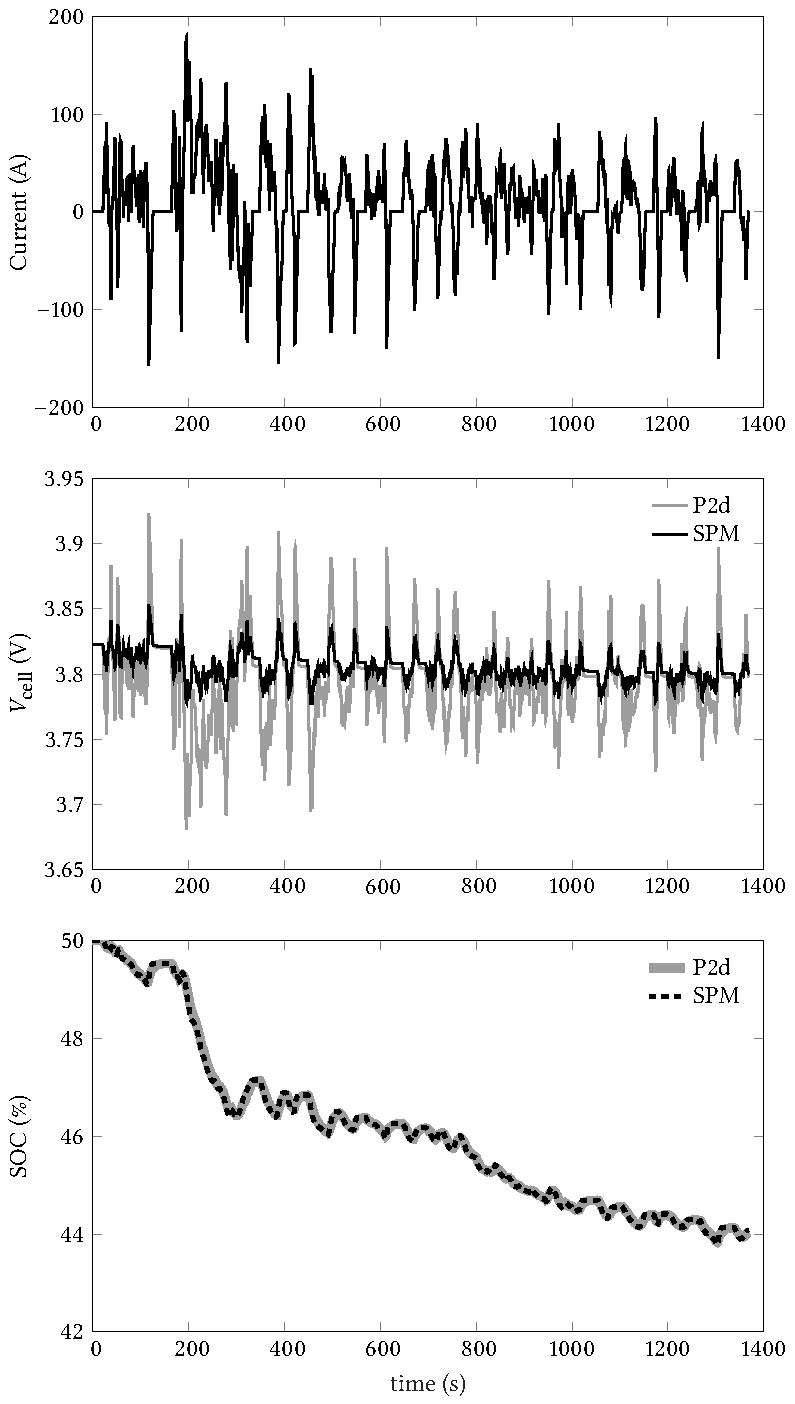
\includegraphics[width=10.890625cm]{udds_I_v_soc.pdf} % change the width suitably afterwards
    \caption[Simulation results of \glsfmtshort{p2d} and \glsfmtshort{spm}
    models to \glsfmtshort{udds} current profile]{Simulation results for a
        \glsfmtshort{udds} current profile. The voltage prediction performance
        of the \glsfmtshort{spm} to dynamic loads is poor while its
    \glsfmtshort{soc} computation accuracy is high.}
    \label{fig:uddssimp2dspmresults}
\end{figure}

\Cref{fig:uddssimp2dspmresults}  shows   the  simulation  results   obtained  by
applying   the   \gls{udds}   current   input  profile   (top   row)   to   both
the   \gls{p2d}   and  \gls{spm}   models.   The   simulation  is   started   at
\SI{50}{\percent}  cell~\gls{soc}. This  is representative  of the  median point
for  the  operating   window  of  \gls{soc}  swing  for   both  \glspl{bev}  and
\glspl{phev}~\cite{Maksimovic2012}. Although  regenerative braking  is employed,
due  to  the  reduced  occurrence  of braking  events  as  well  as  considering
efficiencies of  the drivetrain, as  with any driveycle, the  \gls{udds} profile
also results in a net-discharge. The  cell's \gls{soc} at the termination of the
\gls{udds} run is \approx\SI{6}{\percent} lower than its starting value.

% \FloatBarrier

The  voltage  output   from  the  models  is  plotted  in   the  middle  row  of
\cref{fig:uddssimp2dspmresults}.  The  bottom row  shows  the  evolution of  the
cell's \gls{soc}  over time. Consistent  with the  error trends observed  in the
constant current discharge and charge simulations, the error in terminal voltage
is  high whereas  that in  \gls{soc} is  low. In  this work,  the voltage  error
metrics  are reported  directly in  units  of \si{\milli\volt}  for the  dynamic
simulation run. Furthermore,  it is a standard practice to  report the \gls{rms}
error for such dynamic load profiles and is therefore included in the summary of
error metrics reported in \cref{tbl:errorsummaryuddsdischgspmp2d}.

% -*- root: ../../main.tex -*-
%!TEX root = ../../main.tex
% this file is called up by main.tex
% content in this file will be fed into the main document
% vim:nospell

\begin{table}[!htbp]
    \caption[Error-metrics summary of basic \glsfmtshort{spm} for \glsfmtshort{udds} current profile]{Summary of error
        metrics  of the basic \glsfmtshort{spm} with  \glsfmtshort{udds} input profile.}
    \label{tbl:errorsummaryuddsdischgspmp2d}
    \centering
    \begin{tabular}{@{} l S S @{}} \toprule
        {Error metric} & {$\varepsilon_v\, (\si{\milli\volt})$} & {$\varepsilon_\text{soc}\, (\si{\percent})$} \\ \midrule
        {Abs.\ max.}   & 97.37                                  & 0.21                                         \\
        {\gls{mae}}    & 19.38                                  & 0.04                                         \\
        {\gls{rms}}    & 25.88                                  & 0.06                                         \\ \bottomrule
    \end{tabular}
\end{table}


% accuracy comparison, figure inset

% textwidth in cm: \printinunitsof{cm}\prntlen{\textwidth} % 15.74776 cm
% textheight in cm: \printinunitsof{cm}\prntlen{\textheight} % 22.27184 cm
% github toolbox


% % Table comparing simulation speeds for cts and disc for constant current and dynamic current


\section{Quadratic Approximation of Ionic Spatial Concentration}\label{sec:quadraticapprox}
% -*- root: ../../main.tex -*-
%!TEX root = ../../main.tex
% this file is called up by main.tex
% content in this file will be fed into the main document
% vim:textwidth=80 fo=cqt

As  evidenced by  the  results from  constant  current  charge, discharge  and
dynamic  simulation runs presented in \cref{sec:basicspmsimresults},  the basic 
\gls{spm} suffers  from poor voltage accuracy. The prior art discussed in
\cref{sec:electrolyteinclusion} aim to tackle this issue through inclusion of
electrolyte dynamics using various state of the art methods. However, they lack
in providing an in-depth analysis and expository illustration of the fundamental
deficiency of the standard \gls{p2d} dynamics, which is uncovered later in
\cref{subsec:symbolicreg}. This is facilitated through the introduction of the
quadratic approximation model of ionic spatial concentration in this
section\footnote{The  mathematical derivations  here  represents  the  author's 
    digested  summary  of  literature, and  is  particularly  based  upon  a 
portion  of  Deng~\etal~\cite{Deng2018}}. The quadratic approximation model is
notable since it serves as the baseline reference for inclusion of electrolyte
dynamics into an \gls{spm}.

% The  steps  involved  in  deriving   the  quadratic  approximation  is  detailed
% in  \cref{subsec:quadraticmodelderiv}.  Based  on   the  results  from  applying
% this   quadratic   approximation   scheme,   an   analysis   of   the   weakness
% of  this   model  is  performed   in  \cref{subsec:quadraticsimresultsanalysis}.

% Mitigation  of   this  critical  drawback   lead  to  this   author's  decoupled
% spatio-temporal electrolyte concentration model  structure which is presented in
% \cref{sec:newelectrolytemodel}.

\subsection{Model derivation}\label{subsec:quadraticmodelderiv}

The  schematic  in  \cref{fig:coordsquadapprox}  shows  the  definition  of  the
co-ordinate  systems  used  in  deriving the  polynomial  approximation  of  the
electrolyte  concentration   profile.  The  three   regions~${\{\text{neg,  sep,
pos}\}}$  are  abbreviated  to ${\{n,s,p\}}$~respectively  in  all  mathematical
expressions. The globally defined $x$~co-ordinate starts at the negative current
collector interface~(${x=0}$)  and terminates at the  positive current collector
interface  ($x  = l_\text{tot},\,  \text{where  }  l_\text{tot} =  l_\text{n}  +
l_\text{s} + l_\text{p}$). Three local co-ordinate systems~$z$ valid only within
their respective regions are also defined.  In particular, it must be noted that
the direction of  the local $z_\text{pos}$~co-ordinate axis is  opposite to that
of the other two local co-ordinate axes as well as the global co-ordinate axis.

% In subsequent usages, the  suffix in~$z_\mu$  is dropped  and  the  reader is  advised  to infer  the region  of  validity from  the  usage  context  which  are unambiguous  as  they occur  in separate  equations.

% The author is  convinced that this notation  does not
% detract  from following  the  derivations, but  rather aids  it  by keeping  the
% notations compact.

\begin{figure}[!htbp]
    \captionsetup{singlelinecheck=off}
    \centering
    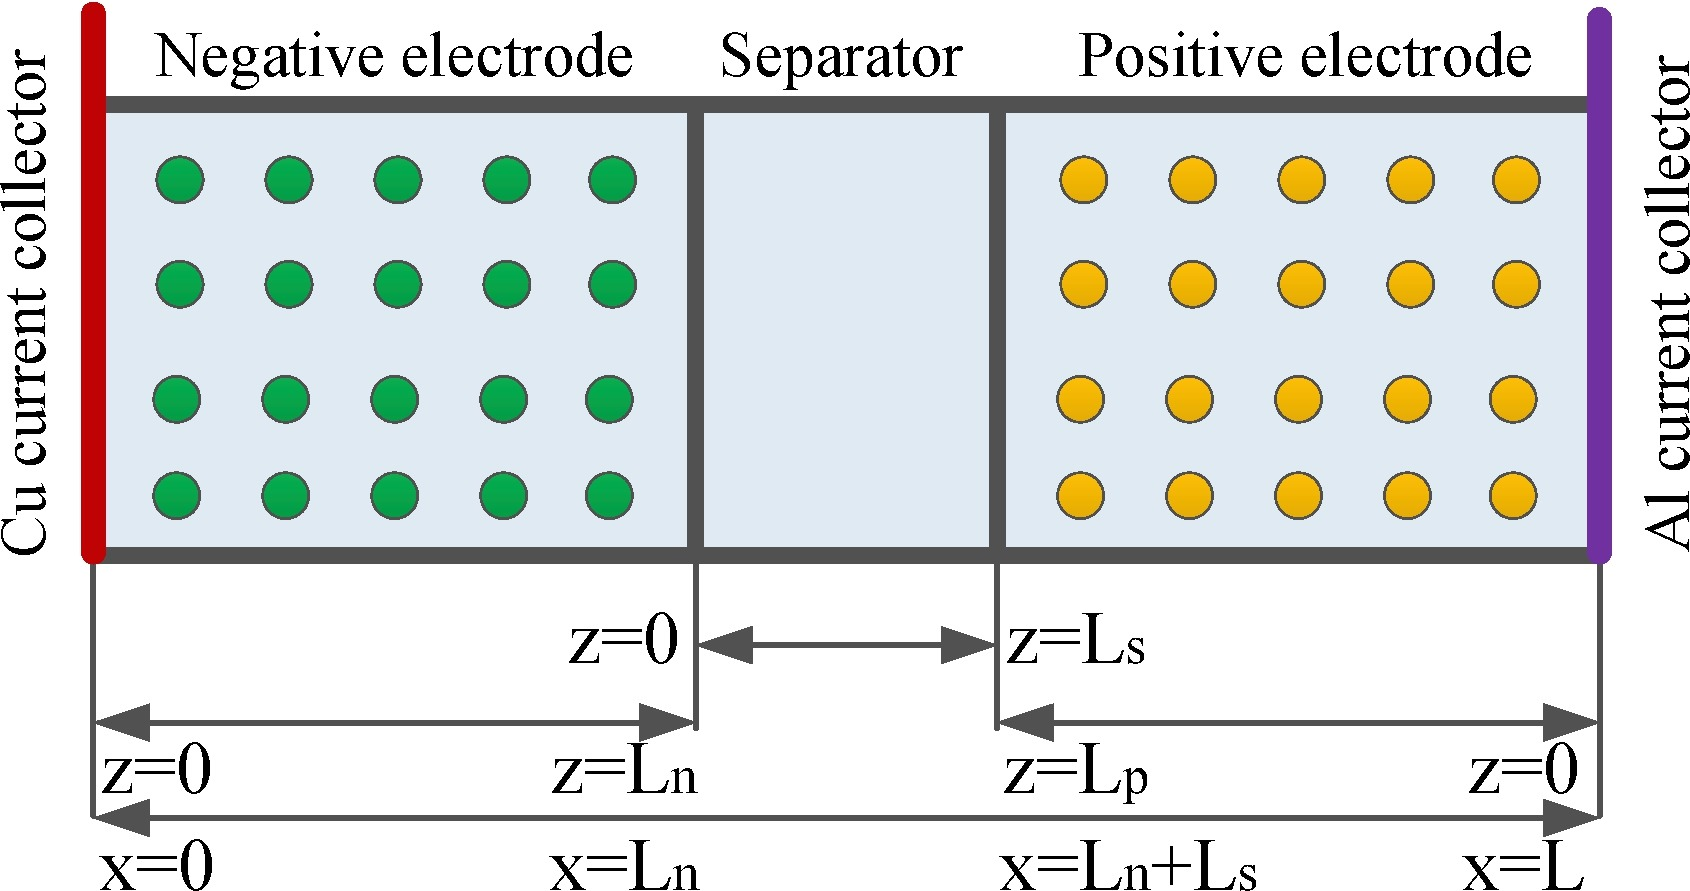
\includegraphics{co_ord_sys}
    \caption[Co-ordinate systems for quadratic approximation of
    electrolyte concentration]{Schematic diagram of the electrochemical sandwich
        consisting of
        \begin{enumerate*}[label=\itshape\alph*\upshape)]
            \item negative electrode,
            \item separator, and
            \item positive electrode
        \end{enumerate*} depicting the co-ordinate system used in deriving the
        quadratic approximation profile. The global spatial co-ordinate is~${x
            \in \{0,L\}}$, where~${L = l_\text{tot} = l_\text{neg} + l_\text{sep} +
        l_\text{pos}}$. Local co-ordinate systems~$z$ specific to each
        region are also defined. It should be noted that the positive
        electrode's local co-ordinate axis direction is reversed with respect to
        the global co-ordinate axis. Illustration reproduced from
    Deng~\etal~\cite{Deng2018}.}
    \label{fig:coordsquadapprox}
\end{figure}

A  standard  quadratic  expression  is chosen  a~priori  for  approximating  the
electrolyte  concentration  profile  within each  region.
\begin{alignat}{2}  %
    % \SwapAboveDisplaySkip
   c_\ensub(z,t) & = a_2(t) z^2  + a_1(t) z + a_0(t) \qquad     &  & 0 \le z \le l_\text{n}\label{eq:cenqquadstart} \\
   c_\essub(z,t) & = a_5(t) z^2 + a_4(t) z + a_3(t) \qquad      &  & 0 \le z \le l_\text{s}\label{eq:cesqquadstart} \\
   c_\epsub(z,t) & =  a_8(t) z^2  + a_7(t)  z  + a_6(t)  \qquad &  & 0  \le z  \le l_\text{p}\label{eq:cepqquadstart}
\end{alignat}
The time-dependent coefficient  vector ${\vec{a}(t) = \vect{a_0(t),a_1(t),
\dots ,a_8(t)}}$ is to be determined\footnotemark.
\footnotetext{Hereafter, the  explicit  time-dependence  of  the
coefficients  is  omitted.  Similarly,  the  spatio-temporal
dependence of the electrolyte  concentration~$c_{\text{e,}j}$ is also dropped
from the notation.}
Applying     boundary     conditions     of    the     electrolyte     diffusion
equation   from   the   \gls{dfn}   model~(refer   \cref{eq:dfnliquiddiff})   to
\crefrange{eq:cenqquadstart}{eq:cepqquadstart},  it is  clear that  ${a_1 =  0}$
and~${a_7 = 0}$. Thus, \crefrange{eq:cenqquadstart}{eq:cepqquadstart} become
\begin{alignat}{2}
    % \SwapAboveDisplaySkip
    c_\ensub      & = a_2 z^2 + a_0         \qquad          &  & 0 \le z \le l_\text{n}\label{eq:cenquadreduced} \\
    c_\essub      & = a_5 z^2 + a_4 z + a_3 \qquad          &  & 0 \le z \le l_\text{s}\label{eq:cesquadreduced} \\
    c_\epsub      & = a_8 z^2 + a_6         \qquad          &  & 0 \le z \le l_\text{p}\label{eq:cepquadreduced}
\end{alignat}
with  the  coefficient  vector being  modified  to~${\vec{a} = \vect{a_0,a_2, \dots ,a_6, a_8}}$.


\Cref{tbl:dfnelectrolyteeqnsinsep} lists  the equations and  boundary conditions
for phenomena  describing electrolyte  diffusion and  charge balance  within the
separator domain.

% -*- root: ../main.tex -*-
%!TEX root = ../main.tex
% this file is called up by main.tex
% content in this file will be fed into the main document
% vim:nospell textwidth=180 foldlevelstart=3 foldlevel=3 conceallevel=0

\begin{table}[!htbp]
    \centering
    \caption[Electrolyte equations \& boundary conditions of \glsfmtshort{dfn} model in separator]{Electrolyte-specific governing equations and boundary conditions of the \glsfmtlong{dfn}~(\glsfmtshort{dfn}) model within the separator domain.}
    \label{tbl:dfnelectrolyteeqnsinsep}
    \begingroup
    \makeatletter\def\f@size{9.25}\check@mathfonts
    \addtolength{\jot}{0.875em}
    \begin{tabular*}{\textwidth}{@{} l c r l r @{}}
        \toprule
        \multicolumn{1}{c}{\small Region} & \small Governing equations & \multicolumn{2}{c}{\small Boundary conditions } & {} \\
        {} & {} & \multicolumn{2}{c}{\scriptsize $(l_\text{neg} \coloneqq l_\text{n},\, l_\text{sep} \coloneqq l_\text{s},\, l_\text{pos} \coloneq l_\text{p})$} \\
        \midrule
        \multicolumn{1}{l |}{{\rotatebox[origin=c]{90}{\makecell{\footnotesize Separator\\ \scriptsize $\delta \in \{\text{sep}\}$}}}} &
        $\begin{aligned}
            \vphantom{D_{\text{\tiny eff}_\text{n}}\!\! \! \!\, \diffp{c_\text{e}}{x}{\mathrlap{x = l^{-}_\text{n}}}} \varepsilon_\delta \diffp{c_\text{e}}{t} &=D_\effdelta  \diffp[2]{c_\text{e}}{x} \\[-0.75em]
            \vphantom{D_{\text{\tiny eff}_\text{s}}\!\! \! \!\, \diffp{c_\text{e}}{x}{\mathrlap{x=(l_{\text{n}} + l_\text{s})^{-}}}}\\[1.25em]
            \vphantom{\kappa_{\text{\tiny eff}_\text{n}}\!\! \! \!\, \diffp{c_\text{e}}{x}{\mathrlap{x = l^{-}_\text{n}}}\hspace{5mm} =\kappa_{\text{\tiny eff}_\text{s}}\!\!\!\!\,\diffp{c_\text{e}}{x}{\mathrlap{x = l^{+}_\text{n}}}} \frac{I}{A} &= \overline{\kappa}_\effdelta \left( \diffp[2]{\phi_\text{e}}{x} + \frac{2 R T}{F} (t^0_{+}-1)\diffp[2]{ \ln c_\text{e}}{x}\right) \\[-0.75em]
            \vphantom{\kappa_{\text{\tiny eff}_\text{s}}\!\! \! \!\, \diffp{c_\text{e}}{x}{\mathrlap{x=(l_{\text{n}} + l_\text{s})^{-}}}} \\
        \end{aligned}$ &
        $\begin{aligned}
    \vphantom{D_{\text{\tiny eff}_\text{n}}\!\! \! \!\, \diffp{c_\text{e}}{x}{\mathrlap{x = l^{-}_\text{n}}}} \qquad c_\text{e}\Bigr\rvert_{\mathrlap{x=l^{-}_\text{n}}}\hspace{5mm} &= c_\text{e}\Bigr\rvert_{\mathrlap{x=l^{+}_\text{n}}},\\[-0.75em]
     \vphantom{\kappa_{\text{\tiny eff}_\text{n}}\!\! \! \!\, \diffp{c_\text{e}}{x}{\mathrlap{x = l^{-}_\text{n}}}\hspace{5mm} =\kappa_{\text{\tiny eff}_\text{s}}\!\!\!\!\,\diffp{c_\text{e}}{x}{\mathrlap{x = l^{+}_\text{n}}}} c_\text{e}\Bigr\rvert_{\mathrlap{x=(l_{\text{n}} + l_\text{s})^{-}}}\hspace{5mm} &= c_\text{e}\Bigr\rvert_{\mathrlap{x=(l_{\text{n}} + l_\text{s})^{+}}},\\[1.25em]
 \vphantom{\kappa_{\text{\tiny eff}_\text{n}}\!\! \! \!\, \diffp{c_\text{e}}{x}{\mathrlap{x = l^{-}_\text{n}}}} \vphantom{\left( \diffp[2]{\phi_\text{e}}{x} + \frac{2 R T}{F} (t^0_{+}-1)\diffp[2]{ \ln c_\text{e}}{x}\right)} \phi_\text{e}\Bigr\rvert_{\mathrlap{x=l^{-}_\text{n}}}\hspace{5mm} &= \phi_\text{e}\Bigr\rvert_{\mathrlap{x=l^{+}_\text{n}}},\\[-0.75em]
 \vphantom{\kappa_{\text{\tiny eff}_\text{s}}\!\! \! \!\, \diffp{c_\text{e}}{x}{\mathrlap{x=(l_{\text{n}} + l_\text{s})^{-}}}} \phi_\text{e}\Bigr\rvert_{\mathrlap{x=(l_{\text{n}} + l_\text{s})^{-}}}\hspace{5mm} &= \phi_\text{e}\Bigr\rvert_{\mathrlap{x=(l_{\text{n}} + l_\text{s})^{-}}},\\
    \end{aligned}$ &
    $\begin{aligned}
        \quad D_{\text{\tiny eff}_\text{n}}\!\! \! \!\, \diffp{c_\text{e}}{x}{\mathrlap{x = l^{-}_\text{n}}}\hspace{5mm} &=D_{\text{\tiny eff}_\text{s}}\!\!\!\!\,\diffp{c_\text{e}}{x}{\mathrlap{x = l^{+}_\text{n}}}\\[-0.75em]
        D_{\text{\tiny eff}_\text{s}}\!\! \! \!\, \diffp{c_\text{e}}{x}{\mathrlap{x=(l_{\text{n}} + l_\text{s})^{-}}}\hspace{5mm} &=D_{\text{\tiny eff}_\text{p}}\!\!\!\!\,\diffp{c_\text{e}}{x}{\mathrlap{x=(l_{\text{n}} + l_\text{s})^{+}}}\\[1.25em]
        \vphantom{\left( \diffp[2]{\phi_\text{e}}{x} + \frac{2 R T}{F} (t^0_{+}-1)\diffp[2]{ \ln c_\text{e}}{x}\right)} \kappa_{\text{\tiny eff}_\text{n}}\!\! \! \!\, \diffp{c_\text{e}}{x}{\mathrlap{x = l^{-}_\text{n}}}\hspace{5mm} &=\kappa_{\text{\tiny eff}_\text{s}}\!\!\!\!\,\diffp{c_\text{e}}{x}{\mathrlap{x = l^{+}_\text{n}}}\\[-0.75em]
        \kappa_{\text{\tiny eff}_\text{s}}\!\! \! \!\, \diffp{c_\text{e}}{x}{\mathrlap{x=(l_{\text{n}} + l_\text{s})^{-}}}\hspace{5mm} &=\kappa_{\text{\tiny eff}_\text{p}}\!\!\!\!\,\diffp{c_\text{e}}{x}{\mathrlap{x=(l_{\text{n}} + l_\text{s})^{+}}}\\
    \end{aligned}$ &
    $\begin{aligned}
        \vphantom{D_{\text{\tiny eff}_\text{n}}\!\! \! \!\, \diffp{c_\text{e}}{x}{\mathrlap{x = l^{-}_\text{n}}}} \quad \refstepcounter{equation}(\theequation)\label{eq:liquiddiffnsep} \\[-0.75em]
        \vphantom{D_{\text{\tiny eff}_\text{s}}\!\! \! \!\, \diffp{c_\text{e}}{x}{\mathrlap{x=(l_{\text{n}} + l_\text{s})^{-}}}}\\[1.25em]
        \vphantom{\kappa_{\text{\tiny eff}_\text{n}}\!\! \! \!\, \diffp{c_\text{e}}{x}{\mathrlap{x = l^{-}_\text{n}}}} \vphantom{\left( \diffp[2]{\phi_\text{e}}{x} + \frac{2 R T}{F} (t^0_{+}-1)\diffp[2]{ \ln c_\text{e}}{x}\right)} \refstepcounter{equation}(\theequation) \label{eq:liquidpotentialsep}\\[-0.75em]
        \vphantom{\kappa_{\text{\tiny eff}_\text{s}}\!\! \! \!\, \diffp{c_\text{e}}{x}{\mathrlap{x=(l_{\text{n}} + l_\text{s})^{-}}}}
    \end{aligned}$
    \\
    \bottomrule
\end{tabular*}
\endgroup
\end{table}



\Cref{eq:liquiddiffnsep}  and   \cref{eq:liquidpotentialsep}  are   obtained  by
applying   the  pertinent   electrolyte   equations  of   the  \gls{dfn}   model
(\cref{eq:dfnliquiddiff} and  \cref{eq:dfnliquidpotential} respectively)  to the
separator  region. Applying  the continuity  and flux  boundary conditions  from
\cref{eq:liquiddiffnsep} at both separator interfaces,
\begin{alignat}{2}
    \SwapAboveDisplaySkip
    \allowdisplaybreaks
    a_2 l^2_\text{n} + a_0                      & = \hphantom{-}a_3 \qquad                    &  & \text{\footnotesize (continuity at neg/sep interface)} \label{eq:cecontinuitynegsep} \\
    a_5 l^2_\text{s} + a_4 l_\text{s} + a_3     & = \hphantom{-}a_8 l^2_\text{p} + a_6 \qquad &  & \text{\footnotesize (continuity at sep/pos interface)}                               \\
    2 a_2 l_\text{n} D_\effn                    & = \hphantom{-}a_4 D_\effs \qquad            &  & \text{\footnotesize (flux b.c.\ at neg/sep interface)}                               \\
    \left(2 a_5 l_\text{s} + a_4\right) D_\effs & = -2 a_8 l_\text{p} D_\effp \qquad          &  & \text{\footnotesize (flux b.c.\ at sep/pos interface)}\label{eq:quadcefluxseppos}
\end{alignat}
The negative sign in \cref{eq:quadcefluxseppos} is due to the specific
choice of  the co-ordinate system  used for  the positive electrode  region (see
\cref{fig:coordsquadapprox}).  Due to  this,  fluxes  at the  separator/positive
electrode interface have opposing directions.
Let  $Q_\text{e,j}$  denote  the  number  of moles  of  \ch{Li^+}~ions  in  the
electrolyte per  unit cross-sectional  area within each  region~$\jinnegseppos$.
This is  computed as  the product  of
\begin{enumerate*}[label=\emph{\alph*})]
    \item the porosity and
    \item spatial integral of the concentration function
\end{enumerate*}
\ie~${ Q_\text{e,j}  =  \varepsilon_j \int_0^{l_j}  c_{\text{e},j}(z) \,dz  }$.
Applying this to \crefrange{eq:cenquadreduced}{eq:cepquadreduced}
\begin{align}
    Q_\text{e,n} &= \varepsilon_\text{n} \left( \frac{1}{3} a_2 l^3_\text{n} + a_0 l_\text{n}\right)\label{eq:Qenbyintegration}\\
    Q_\text{e,s} &= \varepsilon_\text{s} \left( \frac{1}{3} a_5 l^3_\text{s} + \frac{1}{2} a_4 l^2_\text{s} + a_3 l_\text{s}\right)\\
    Q_\text{e,p} &= \varepsilon_\text{p} \left( \frac{1}{3} a_8 l^3_\text{p} + a_6 l_\text{p}\right) \label{eq:Qepbyintegration}
\end{align}

\addlines
At this stage,  $Q_{\text{e},j}(t)$~are unknown. Since  these are time-dependent
functions,  the  derivation  naturally  progresses  towards  seeking  a  set  of
\glspl{ode} that describe a relationship  for their time evolution. Transforming
the  \engordnumber{2}   order  \glspl{ode}  of \cref{eq:dfnliquiddiff}   (for  electrodes)
and \cref{eq:liquiddiffnsep}   (for  separator)   to   their  respective   local
co-ordinates and integrate  once along the thickness of  each region. Performing
this sequence of steps for the negative electrode region
\mathleft
\begin{equation}
    \begin{WithArrows}[b]
        \varepsilon_\text{n} \int_0^{l_\text{n}} \left(\diffp*{c_\ensub(z,t)}{t}\right)\, dz &= \int_0^{l_\text{n}} \left(\diffp{}{z}\left(D_\effn \diffp{c_\ensub}{z} \right) + (1 - t^0_\text{+}) a_\snsub j_\text{n}\right)\, dz \Arrow[tikz={text width=3.4cm}]{transposing integration \& differentiation operations in the \glsfmtshort{lhs}} \\
        \varepsilon_\text{n} \diffp*{\int_0^{l_\text{n}} c_\ensub(z,t)}{t}\, dz &=
        \int_0^{l_\text{n}} \left(\diffp{}{z}\left(D_\effn \diffp{c_\ensub}{z}
        \right) + (1 - t^0_\text{+}) a_\snsub j_\text{n}\right)\, dz
        \Arrow[tikz={text width=3.4cm}]{apply time-derivative operator to the whole \glsfmtshort{lhs}}\\
        \diffp*{\left(\tikzmark{StartBraceA}\varepsilon_\text{n} \int_0^{l_\text{n}}
c_\ensub(z,t)\, dz\tikzmark{EndBraceA}\right)}{t} &=  \int_0^{l_\text{n}}
\left(\diffp{}{z}\left(D_\effn \diffp{c_\ensub}{z} \right) + (1 -
    t^0_\text{+}) a_\snsub j_\text{n}\right)\, dz \Arrow[tikz={text
width=3.4cm}]{apply integral to the \glsfmtshort{rhs}}\\
        \diff*{Q_\text{e,n}(t)}{t} &= D_\effn \diffp{c_\ensub}{z}{\mathrlap{z=l_\text{n}}} + (1 - t^0_\text{+}) a_\snsub \int_0^{l_\text{n}} j_\text{n}\, dz
    \end{WithArrows}
    \label{eq:negliionmolestoreduce}
\end{equation}
\mathcenter
\InsertUnderBrace[draw=black][aspect=0.26]{StartBraceA}{EndBraceA}{} % https://tex.stackexchange.com/questions/68526/asymmetric-overbrace
% \blindtext
% \AddToShipoutPicture*{\ShowFramePicture}
Performing     the     identical     sequence     of     operations     starting
from~(\cref{eq:liquiddiffnsep}) for  the separator and~(\cref{eq:dfnliquiddiff})
for the positive electrode yields
\begin{align}
    % \SwapAboveDisplaySkip
    \diff*{Q_\text{e,s}(t)}{t} &= D_\effs \diffp{c_\essub}{z}{\mathrlap{z=l_\text{s}}} \label{eq:sepliionmolestoreduce}\\
    \diff*{Q_\text{e,p}(t)}{t} &= D_\effp \diffp{c_\epsub}{z}{\mathrlap{z=l_\text{p}}} + (1 - t^0_\text{+}) a_\spsub \int_0^{l_\text{p}} j_\text{p}\, dz\label{eq:posliionmolestoreduce}
\end{align}

In    order    to   evaluate    the    integral    term   in    the    \gls{rhs}
of \cref{eq:negliionmolestoreduce}    and \cref{eq:posliionmolestoreduce},   the
solid  phase  charge  conservation  equation~(\cref{eq:solidchargeconserve})  is
integrated  along the  local  co-ordinate  axis of  the  negative electrode  and
positive electrode respectively.
\begin{align}
    \int_0^{l_\text{n}} j_\text{n}\, dz & =  \frac{I}{a_\snsub A F} \label{eq:negfluxintegral}\\
    \int_0^{l_\text{p}} j_\text{p}\, dz & =  \frac{-I}{a_\spsub A F}\label{eq:posfluxintegral}
\end{align}

Substituting       \crefrange{eq:negfluxintegral}{eq:posfluxintegral}       into
\crefrange{eq:negliionmolestoreduce}{eq:posliionmolestoreduce} respectively,
\begin{align}
    \allowdisplaybreaks
    \diff*{Q_\text{e,s}}{t} &= D_\effn \diffp{c_\ensub}{z}{\mathrlap{z=l_\text{n}}} - (1 - t^0_\text{+}) \cancel{a_\snsub} \frac{I}{\cancel{a_\snsub} A F} \\
    \diff*{Q_\text{e,p}}{t} &= D_\effp \diffp{c_\epsub}{z}{\mathrlap{z=l_\text{p}}} - (1 - t^0_\text{+}) \cancel{a_\spsub} \frac{-I}{\cancel{a_\spsub} A F}
\end{align}
which leads to the general expressions  for the cross-sectional molar density of
\ch{Li^+}~ions in each of the three regions as
\begin{align}
    \diff*{Q_\text{e,n}}{t} & = D_\effn \diffp{c_\ensub}{z}{\mathrlap{z=l_\text{n}}} + (1 - t^0_\text{+}) \frac{I}{A F} \label{eq:negliionmolesgen} \\
    \diff*{Q_\text{e,s}}{t} & = D_\effs \diffp{c_\essub}{z}{\mathrlap{z=l_\text{s}}} \label{eq:sepliionmolesgen}                                             \\
    \diff*{Q_\text{e,p}}{t} & = D_\effp \diffp{c_\epsub}{z}{\mathrlap{z=l_\text{p}}} - (1 - t^0_\text{+}) \frac{I}{A F}\label{eq:posliionmolesgen}
    \intertext{Substituting the assumed quadratic expressions for electrolyte concentrations in
        each of the three regions \crefrange{eq:cenquadreduced}{eq:cepquadreduced}
    in the above system \ie~\crefrange{eq:negliionmolesgen}{eq:posliionmolesgen}}
    \diff*{Q_\text{e,n}}{t} & = 2 a_2 l_\text{n} D_\effn + (1 - t^0_\text{+}) \frac{I}{A F} \label{eq:negliionmolesquadratic}                                \\
    \diff*{Q_\text{e,s}}{t} & = 2 a_5 l_\text{s} D_\effs\label{eq:sepliionmolesquadratic}                                                                                                     \\
    \diff*{Q_\text{e,p}}{t} & = 2 a_8 l_\text{p} D_\effp - (1 - t^0_\text{+}) \frac{I}{A F} \label{eq:posliionmolesquadratic}
\end{align}
\addlines
The  initial   ionic  concentration   in  the   electrolyte  is   identical  in
all  three  regions  of  the  cell,  assuming  equilibrium  starting  conditions
\ie~${c_{\text{e,0}_j}  = c_\text{e,0},  \jinnsp}$.  Hence the  initial number  of
moles of \ch{Li^+} per unit area in each of the three regions is given by
\begin{align}
    Q_\text{e,n}(0) & = \varepsilon_\text{n} c_\text{e,0} l_\text{n} \label{eq:Qeninit}\\
    Q_\text{e,s}(0) & = \varepsilon_\text{s} c_\text{e,0} l_\text{s}\\
    Q_\text{e,p}(0) & = \varepsilon_\text{p} c_\text{e,0} l_\text{p} \label{eq:Qepinit}\\
    \intertext{and the initial coefficient vector which satisfies the system
    equations is obtained as}
    \begin{bmatrix}
        a_0 \\
        a_2 \\
        a_3 \\
        a_4 \\
        a_5 \\
        a_6 \\
        a_8
        \end{bmatrix} & = \begin{bmatrix}
        c_\text{e,0} \\
        0 \\
        c_\text{e,0} \\
        0 \\
        0 \\
        c_\text{e,0} \\
        0
    \end{bmatrix} \label{eq:coeffinit}
\end{align}

The             system             of             three             \glspl{ode},
\eqref{eq:negliionmolesquadratic}--\eqref{eq:posliionmolesquadratic}    together
with  \crefrange{eq:Qeninit}{eq:Qepinit}  representing the  initial  conditions,
form   an    \gls{ivp}.   \Crefrange{eq:cecontinuitynegsep}{eq:Qepbyintegration}
represent a square system of seven linear algebraic equations with seven unknown
coefficients which must be solved at each time-step. These algebraic constraints
coupled with the aforementioned \gls{ivp} form a \gls{dae} system.

There are now two choices for proceeding  with solution of the system. The naive
approach  would be  to  solve  the \gls{dae}  using  advanced \gls{dae}  solvers
specially designed to handle \mbox{index-1}  semi-explicit systems such as
DASSL~\cite{Petzolddassl}
and  DASPK~\cite{VanKeken1995}. For  start-stop  type  of input  currents  with discontinuities,  the
consistent initialisation of algebraic conditions and derivatives is numerically
challenging.  All   \gls{dae}  solvers  typically  use   adaptive  time-stepping
algorithms.  The  feasibility of  using  such  a  complex scheme  for  real-time
computation is questionable. On the other hand, the overall system can be viewed
as composed of two numerical subsystems ---
\begin{enumerate*}[label=\emph{\alph*})]
    \item an independent \gls{ode} system, and
    \item an independent algebraic system.
\end{enumerate*}
Each system  is executed  back to  back in succession  using solutions  from the
other system from the previous time-step.

To  clarify  the sequence  of  operations,  in  order  to bootstrap  the  model,
it  is  required  to  compute  $Q_{\text{e},j}(t)$ in  all  three  regions.  The
\gls{ode} system is  integrated for one time-step by  retaining the coefficients
at  their initial  value.  The $Q_{\text{e},j}(t)$  thus  solved is  substituted
into  the  algebraic system  to  yield  the  updated  value of  the  coefficient
vector~$\vec{a}(t=t_k)$. This new value of the coefficient vector is substituted
back  into  the  \gls{ode}  system  and  the  process  continues.  Although  the
continuous simulation of  the overall \gls{dae} is not accomplished,  this scheme is
pragmatic from an engineering viewpoint. This is because,  the periodic pauses needed to update
the intertwined  sub-systems translate  naturally into  fixed time-steps  and is
well-suited for a \gls{bms} controller operating at a fixed sample rate. This is
also an effective workaround to mitigate the complexities of having to implement
and solve \glspl{dae} in real time.

% need to write algorithm
The   simulation   results   of   the   quadratic   approximation   scheme   and
the   analysis   of   its   strengths   and   weaknesses   is   presented   next
in \cref{subsec:quadraticsimresultsanalysis}.

\subsection{Numerical implementation, simulation results and analysis}\label{subsec:quadraticsimresultsanalysis}

\subsubsection*{Numerical implementation}
From an analysis point of view,  the quadratic approximation model for computing
the  spatio-temporal evolution  of  electrolyte concentration  can be  simulated
as  an  independent subsystem,  and  hence  can  be implemented  numerically  as
a  standalone  module as  shown  in  \cref{alg:quadraticce}. In  practice,  this
modular code  is embedded as  a subroutine within  the main \gls{spm}  loop (see
\cref{alg:disctimespm}).

% -*- root: ../main.tex -*-
%!TEX root = ../main.tex
% this file is called up by main.tex
% content in this file will be fed into the main document
% vim:nospell

\begin{algorithm}[!htbp]
    \caption{Quadratic approximation model for spatio-temporal electrolyte concentration}\label{alg:quadraticce}
    \begin{algorithmic}[1]
        \Require Load profile \Comment{\eg~a \texttt{csv} file of $t$ vs.\ C-rate}
        \Require Electrolyte model parameter set  \Comment{\eg~stored in a struct \texttt{ceparams}}
        \Userdata $ t_\text{f}$,  sample rate $T_s, c_\text{e,init}$
        \Function{QuadraticElectrolyteModel}{}
        \State Set $Q_{\text{e,init}_j}$ as per \crefrange{eq:Qeninit}{eq:Qepinit}
        \State $\vec{a}[1]$ \gets values from \cref{eq:coeffinit}
        \State $V_\text{cell}[1] \gets \textsc{ComputeCellVoltage}(\textbf{x}[1],I[1],\texttt{params})$ \Comment{from direct feedthrough}
        \For{$k \gets 2 : N_\text{max}$}
        \State $I[k] \gets $ interpolate from profile using \gls{zoh}
        \State Solve continuous-time state equations--\crefrange{eq:negliionmolesquadratic}{eq:posliionmolesquadratic} \Comment{Using $\vec{a}[k-1]$}
        \State $Q_{\text{e}_j}[k]$ \gets last time-entry  vector of soln.\  matrix \Comment{if using an adaptive solver}
        \State $\vec{a}[k]$ \gets solution of \emph{linear} system of equations--\crefrange{eq:cecontinuitynegsep}{eq:Qepbyintegration} \Comment{Using $Q_{\text{e}_j}[k-1]$}
        \State Compute $c_{\text{e}_j}$ as per \crefrange{eq:cenquadreduced}{eq:cepquadreduced} \Comment{Quadratic polynomial expressions for concentration}
        \EndFor
        \EndFunction
    \end{algorithmic}
\end{algorithm}


\begin{figure}[!htb]
    \centering
    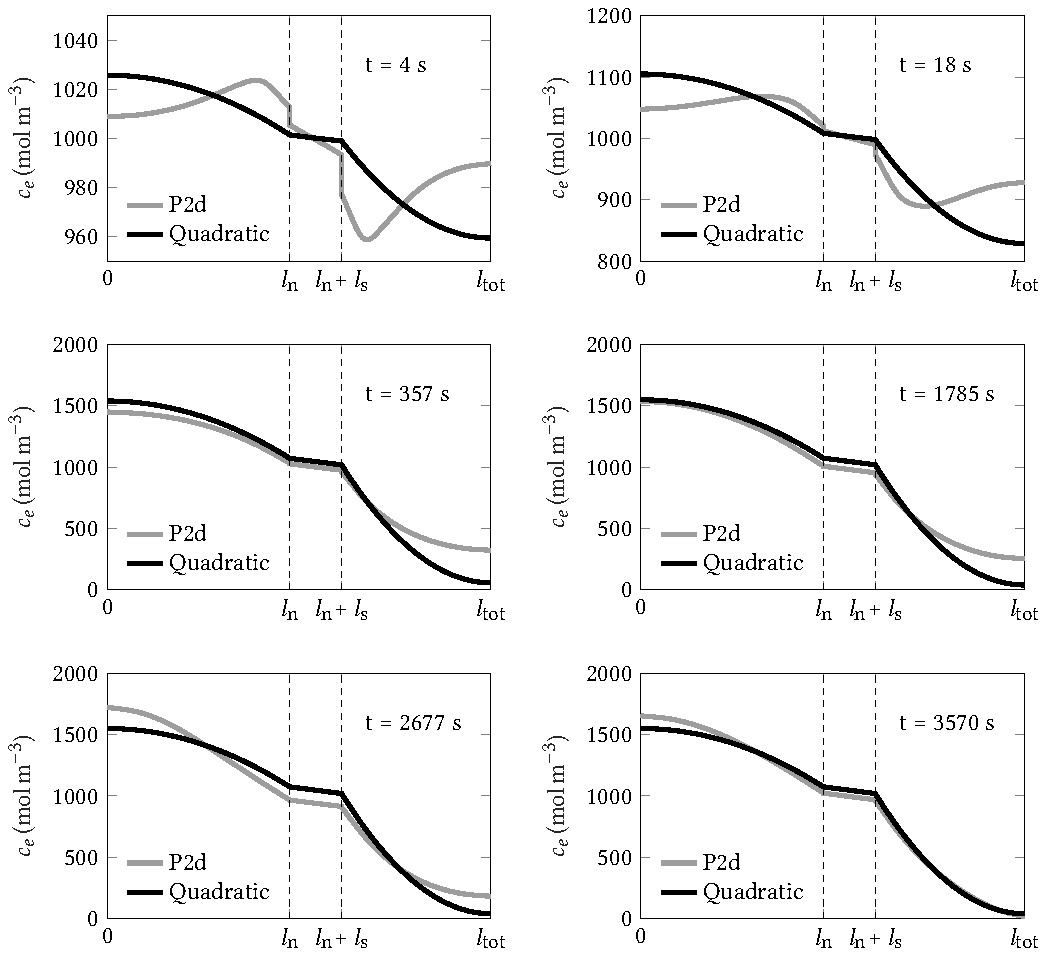
\includegraphics[width=\textwidth]{quadratic_ce_approx_spatial_1C.pdf}
    \caption[Spatial distribution of electrolyte concentration for 1C~discharge]{Spatial distribution of ionic concentration in electrolyte along
        cell thickness at various snapshots of time for a 1C~discharge. The
        concentration profile obtained from simulating the \glsfmtshort{p2d}
        model is used as the reference. The performance of the quadratic model
        is quite poor during the initial transient duration, but improves over
    time as a quasi-steady state is reached.}
    \label{fig:spatialionicconc1C}
\end{figure}


\subsubsection*{Simulation results}\label{subsubsec:simresultsbaselinequad}

\Cref{fig:spatialionicconc1C} shows  the spatial distribution of  \ch{Li^+}~ions
in electrolyte  along the  thickness of  the cell at  various snapshots  of time
obtained by simulation  of the \gls{p2d} and the  quadratic approximation models
using a  1C~discharge current. The  \gls{p2d} model's response is  considered as
the reference benchmark.  During the initial transient  phase, the concentration
profile within each electrode region exhibits a characteristic inflection point.
During this phase,  the concentration profile computed by  the parabolic profile
exhibits  a  large deviation  in  terms  of  percentage  error at  each  spatial
location. However, with the passage of time, as a \gls{qss}~is established, this
inflection point flattens out, and the quadratic approximation becomes closer to
the  true  concentration value  at  each  spatial  location. Similar  trends  in
behaviour is  exhibited for discharge and  charging at higher C-rates  and these
results are  therefore omitted here  in the  interest of keeping  the discussion
succinct.

It  is important  to  note that  while having  a  spatial concentration  profile
is  useful,  as  seen  in \cref{eq:electrolytepdwithce}, it  is  the  values  of
concentration  at   the  \emph{current  collector  interfaces}   that  are  most
influential in  computation of the  electrolyte overpotential and hence,  in the
voltage accuracy of the enhanced \gls{spm}. Thus, it is important to obtain this
alternative perspective  of time-evolution  of the electrolyte  concentration at
the two current collectors.

\begin{figure}[!htbp]
    \centering
    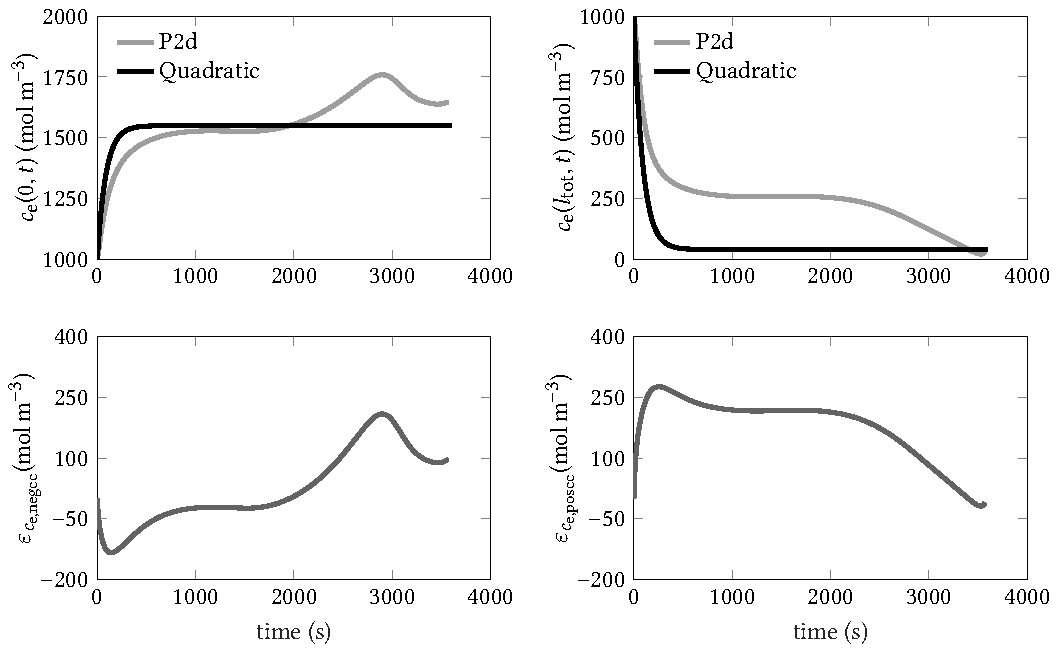
\includegraphics[width=\textwidth]{ce_at_cc_1Cdischg.pdf}
    \caption[Ionic concentrations at current collector
    interfaces over time for 1C~discharge]{Evolution of ionic concentration over
        time at the two current collector interfaces for a 1C~discharge (top
        row). The time evolution of the corresponding error variables is 
    shown in the bottom row of plots.}
    \label{fig:temporalcequadratic}
\end{figure}

\Cref{fig:temporalcequadratic} shows  the time evolution of  ionic concentration
in  the electrolyte  at the  two current  collector interfaces  computed by  the
\gls{p2d} and  quadratic approximation  models for a  1C~discharge  current. The
concentration  values computed  by  the  \gls{p2d} model  is  considered as  the
reference benchmark. At the negative electrode--current collector interface, the
ionic  concentration  exhibits  a  few oscillations  of  small  amplitude  owing
to  the complex  interactions  of  the ionic  phase  with  the porous  electrode
and  the charge  transfer process  at the  electrode-electrolyte boundary.  The
concentration  evolution  predicted  by  the quadratic  approximation  model  is
rather  simplistic  and  is  unable to  capture  this  intricate  time-evolution
pattern.  This  is because  the  governing  equation predicting  time  evolution
of  concentration  in  the  quadratic  approximation  model  is  that  given  by
the  \emph{first-order}  \gls{ode} of \cref{eq:negliionmolesquadratic}  (with  a
proportional mapping from~$Q_\text{e,n}$ to~$c_\text{e}(0,t)$). Following system
theory, the step response  of a first order \gls{ode} is  that of an exponential
rise to a final settling value, which  is exactly the shape seen in the top-left
plot of \cref{fig:temporalcequadratic}.

The ionic  concentration evolution  at the positive  current collector  does not
exhibit major oscillations  and even has a subtle monotonicity  to its response.
However,  the  classical  first  order  response  predicated  by  the  quadratic
approximation model falls short of representing its complete dynamics. Errors of
similar  magnitude  are present  in  the  ionic  concentration at  both  current
collector  interfaces, with  a maximum  absolute error  of \approx\SI{250}{\mole
\per \meter  \cubed}.
% Similar trends are  exhibited in charging, with  a swapped response pattern observed at the two current collector interfaces.



 % Analysis of SPM
\setcounter{chapter}{5}
% -*- root: ../main.tex -*-
%!TEX root = ../main.tex
% this file is called up by main.tex
% content in this file will be fed into the main document
% vim:textwidth=80 fo=cqt

\graphicspath{{chapters/sys_id/figures/}}
% ----------------------- contents from here ------------------------

\clearpage
\chapter{Implementing a New Electrolyte Model for Augmentation of the Basic \glsfmtshort{spm}}\label{ch:newelectrolytemodel}
\startcontents[chapters]
\printcontents[chapters]{}{1}{\setcounter{tocdepth}{1}}

% A suitable  family of models from  the broad category of  reduced-order models
% is  identified  as  a  promising  candidate  for  implementation  in  controls
% applications.
\bigskip

% -*- root: ../main.tex -*-
%!TEX root = ../main.tex
% this file is called up by main.tex
% content in this file will be fed into the main document
% vim:textwidth=80 fo=cqt


\capolettera{T}{his} chapter presents the  author's attempts towards arriving at
an  accurate description  of the  spatio-temporal evolution  of the  electrolyte
concentration. The  performance of the quadratic  approximation model introduced
in \cref{ch:spmanalysis} is analysed through the novel application of a symbolic
regression framework that  helped to expose the issue of  equation deficiency in
the underlying \gls{dfn}  model for the purpose of electrolyte  modelling with a
pre-assumed model  structure. Although this  framework did not  ultimately yield
the desired outcomes, it did nevertheless facilitate a comprehensive analysis of
the strengths and weaknesses of the  quadratic approximation model which has not
been performed in existing literature. Next, the author's unique contribution to
the art  of single  particle modelling  \viz{} a  novel time-evolution  model of
electrolyte  concentrations through  the technique  of system  identification is
presented. The  results of  the new  approach is  compared against  the baseline
quadratic approximation model. Finally, the new model equations are incorporated
into  an electrolyte-enhanced  \gls{spm} and  the performance  of the  composite
model is compared against the conventional \gls{spm},



\section{Performance Analysis: Quadratic Approximation Model}\label{sec:symbolicregression}
% -*- root: ../main.tex -*-
%!TEX root = ../main.tex
% this file is called up by main.tex
% content in this file will be fed into the main document
% vim:textwidth=80 fo=cqt


In the  author's analysis of the  quadratic approximation model, the  origin and
nature of  its sub-optimal  performance can  be explained  as per  the following
rationale. The quadratic  approximation model uses a  bottom-up approach wherein
the final  simplified model structure  is pre-assumed  and then the  physics are
made  to  fit  within  this  framework. Given  that  the  top-down  approach  to
electrolyte  modelling \ie~accounting for  all physical  phenomena and  then
simplifying  them yields  mathematically intractable  and overly  complex models
(see \cref{sec:electrolyteinclusion} for  a detailed discussion),  this approach
seems to be a pragmatic alternative  to enhancing the \gls{spm} with electrolyte
dynamics. However, a detailed look at  this model from an alternate viewpoint is
necessary for further analysis.


\subsection{Symbolic regression using \glsfmtlong{mggp}}\label{subsec:symbolicreg}

The  question boils  down to  whether a  quadratic approximation  is indeed  the
\emph{best}  model structure  that  can  be assumed  a~priori  for the  spatial
profile  of  ionic  concentration  in  the  electrolyte.  This  author  embarked
on  a journey  to  find  suitable alternate  model  structures \ie~a  single
family of  curves that can  capture both  the transient and  \gls{qss} behaviour
exhibited by  the ionic  concentration. The open-source  \textsc{MATLAB} toolbox
GPTIPS2~\cite{Searson2015}  uses the  state-of-the-art  \gls{mggp} approach  for
symbolic data  mining and is ideally  suited for such symbolic  regression tasks
(fitting a  mathematical equation structure,  and not merely  obtaining best-fit
coefficients to a  pre-assumed curve as in classical numerical  regression, to a
given data).

In employing the \gls{mggp} approach, it  is important to recognize that the key
criteria that restricts
\begin{enumerate*}[label=\emph{\alph*})]
    \item the choice of  gene-sequence depth, as well as
    \item the choice in number of parent mutations,
\end{enumerate*}
is  the   total  number  of   unknown  symbolic  coefficients  required   to  be
solved  in the  assumed  model  structure. There  are  a  total of  \emph{seven}
linear   equations  available   from  the   physics  of   the  \gls{dfn}   model
(see \crefrange{eq:cecontinuitynegsep}{eq:Qepbyintegration}). Hence, in order to
guarantee  a solution  the  assumed  family of  curves  cannot  consist of  more
than  seven coefficients.  Furthermore, for  a  unique solution,  the number  of
coefficients must be \emph{exactly} seven. Yet another restriction on the choice
of locus of feasible  curves arises due to the fact that  the behaviour of ionic
concentration  in the  negative and  positive electrode  regions are  similar in
complexity\footnote{\label{fn:complexity}The  concept  of complexity  of  curves
used  here is  not  based on  a  precise mathematical  definition  such as  that
employed by Neumann-Coto and Arenas~\cite{Neumann-Coto2017}, but is loosely used
to simply  convey an empirical sense  of their curvature. However,  the analysis
here applies  to the more  rigorous definition as well.},  and hence need  to be
mathematically described by an identical family of curves.

Upon a close inspection of the  spatial concentration profile from the \gls{p2d}
simulation  results shown  in \cref{fig:spatialionicconc1C}, it  is evident  the
electrolyte approximation  functions within the  electrode regions is  of higher
complexity\textsuperscript{\ref{fn:complexity}} than  the approximation function
suitable  for  use  in  the  separator  region. Based  on  the  results  of  the
quadratic  model, it  is  clear  that at  least  two  coefficients are  required
within the  electrode regions \ie~${n_{\text{c,elec}} \ge 2}$. There  exists an
inhibiting  factor that  prevents  the  use of  a  lower  order function  within
the  separator. As  per  the  simulation results  of  the  \gls{p2d} model,  the
time-domain  change  of number  of  moles  per  square  meter in  the  separator
is  non-zero.  Since  the  time-derivate   of  a  linear  approximation  applied
to \cref{eq:sepliionmolesquadratic}  is  zero,  this straight-line  equation  is
immediately ruled out. Among the  non-polynomial mathematical curves tried (such
as trigonometric, hyperbolic, power series  among others), none could obtain the
relatively simple shape of the separator function without being forced to reduce
the  contribution from  one  of  the coefficients  to  below machine  precision.
This necessitates  the retention  of the  quadratic approximation  function used
thus  far  (with  no  missing  terms) \ie~${n_\text{c,sep}  =  3}$.  Thus,  the
overall number  of coefficients in the  best possible approximation shall  be $2
n_\text{c,elec} + n_\text{c,sep} =  2\cdot2 + 3 = 7$, which  is the total number
of electrolyte-specific physical constraints available from the \gls{dfn} model.
Hence it  can be concluded  that the  quadratic approximation model  does indeed
make the \emph{best}  use of all of the available  physical equations. The final
question remains to  answer is, with these coefficient  limitations, whether the
quadratic  equation structure  indeed  the optimal  one.  This was  investigated
through the \gls{mggp} approach described next.

The GPTIPS2  toolbox uses a variety  of heuristic algorithms from  the theory of
\gls{mggp}  to hypothesise  a suitable  equation structure  for the  data to  be
fitted.  The dataset  consisted of  the  simulation results  from the  \gls{p2d}
model,  in particular  the  values  of electrolyte  concentration  at the  three
different cell  regions captured  at various snapshots  of time.  Both transient
and  \gls{qss} data  were  fed into  this  symbolic data  mining  process and  a
single all-encompassing  family of curves  capable of capturing  the electrolyte
concentration behaviour was  sought for. However, the constraints  in the number
of coefficients that  can be employed results  in a restriction of  the depth of
gene  mutations as  well  as the  number of  parent/seed  populations. The  best
equation set  (without strictly  enforcing the aforementioned  hard constraints,
yet  minimizing  the  distance  to  the constraint  vector)  that  the  symbolic
regression approach yielded was
\begin{alignat}{2}
    c_\ensub(z,t) & = a_2(t) \cosh z^2 + a_1(t) \sinh z + a_0(t) \qquad &  & 0 \le z \le l_\text{n} \label{eq:cnstrviolneg} \\
    c_\essub(z,t) & = a_5(t) z^2 + a_4(t) z + a_3(t) \qquad             &  & 0 \le z \le l_\text{s}                         \\
    c_\epsub(z,t) & = a_8(t) \cosh z^2 + a_7(t) \sinh z + a_6(t) \qquad &  & 0 \le z \le l_\text{p}\label{eq:cnstrviolpos}
\end{alignat}

Although \crefrange{eq:cnstrviolneg}{eq:cnstrviolpos}  fit   the  transient  and
\gls{qss}  profiles  well,  they  violate   the  constraint  on  the  number  of
coefficients  available resulting  in  an underdetermined  system of  equations.
Both  the least-squares  and  least-norm  solution of  this  system were  tried.
However, the  results were inferior to  that produced by the  baseline quadratic
approximation method.

Next, an  attempt was made to  obtain different mathematical structures  for the
transient phase  and \gls{qss}  phase both  of which  respect the  constraint on
number  of  coefficients  allowed.  The symbolic  regression  outputs  for  this
approach are shown in \cref{tbl:symbreg}.
% -*- root: ../../main.tex -*-
%!TEX root = ../../main.tex
% this file is called up by main.tex
% content in this file will be fed into the main document
% vim:nospell textwidth=180 foldlevelstart=3 foldlevel=3 conceallevel=0

\begin{table}[!htbp]
    \centering
    \caption[Transient \& \glsfmtshort{qss} expressions for electrolyte
    concentration obtained by \glsfmtshort{mggp}]{Best fit expressions for the
        transient and \glsfmtlong{qss} approximaton functions for the
    electrolyte functions obtained by the \gls{mggp} approach.}
    \label{tbl:symbreg}
    \begingroup
    \addtolength{\jot}{0.25em}
    \begin{tabular}{@{} c c r @{}}
        \toprule
        \multicolumn{1}{l}{Transient Function} & \multicolumn{1}{c}{\glsfmtlong{qss} Function} & \multicolumn{1}{c}{Region} \\
        \midrule
        $\begin{aligned}
            c_{\text{e,n}_\text{trans}} &= a_1(t) z^6 \ln z^6 + a_0(t) \\
            c_{\text{e,s}_\text{trans}} &= a_4(t) z^2 + a_3(t) z + a_2(t) \\
            c_{\text{e,p}_\text{trans}} &= a_6(t) z^6 \ln z^6 + a_5(t) \\
        \end{aligned}$ &
        $\begin{aligned}
            c_{\text{e,n}_\text{QSS}} &= a_1(t) \sinh z^2 + a_0(t) \\
            c_{\text{e,s}_\text{QSS}} &= a_4(t) z^2 + a_3(t) z + a_2(t) \\
            c_{\text{e,p}_\text{QSS}} &= a_6(t) \sinh z^2 + a_5(t)
        \end{aligned}$ &
        $\begin{aligned}
            &0 \le z \le l_\text{n} \\
            &0 \le z \le l_\text{s} \\
            &0 \le z \le l_\text{p}
        \end{aligned}$
        \\
        \bottomrule
    \end{tabular}
    \endgroup
\end{table}



Although  the equations  from \cref{tbl:symbreg}  produced  a markedly  improved
response during the transient phase,  the performance during the \gls{qss} phase
was merely at par to the baseline quadratic approximation model. This raised the
prospect of  employing a  blended approach, wherein  a model  changeover between
the  transient  and \gls{qss}  was  contemplated.  However,  since there  is  no
precise definition  of what constitutes  the transient phase of  the electrolyte
concentration response, this  approach required some ad-hoc  timing criteria for
correctly  transitioning  between  the  two \gls{mggp}  equation  sets.  Further
complications arise  during dynamic input conditions,  wherein the concentration
profiles are mostly in a state of  flux and could linger for longer durations at
the contiguous  boundary between  transient-like and  \gls{qss}-like behaviours.
In  the  interest  of  reproducibility  across  different  cell-chemistries  and
corresponding parameter sets, the proposed blended model transition approach was
not further pursued.

Overall,  the  long  and  arduous  process of  symbolic  regression  was  not  a
definitive  success in  this  case  mainly due  to  the  limitation of  equation
deficiency of  physical constraints.  Perhaps if  yet another  \gls{pbm}, \ie~an
alternative  to  the widely  prevalent  \gls{dfn}  model,  can  be used  as  the
baseline,  a  few more  physical  governing  equations  could possibly  be  made
available.  This  can  perhaps  result   in  a  less  restrictive  gene-set  for
coefficient  determination  and  consequently  pave the  way  for  a  successful
implementation  through  this  hitherto  unexplored  route  of  \gls{mggp}-based
equation synthesis.

In conclusion,  the quadratic model for  electrolyte concentration approximation
makes the  best use of the  available physical equations. Given  the constraints
with  respect to  physical equations  discussed here,  it is  also deemed  to be
the  optimum  family  of  a~priori  chosen  curves  capable  of  modelling  the
\emph{spatial}  profile of  ionic concentration.  Notwithstanding these  merits,
the  \emph{temporal}  performance of  the  quadratic  approximation approach  is
sub-optimal as seen in \cref{fig:temporalcequadratic}. The author of this thesis
addresses this specific issue with a completely different approach that shall be
discussed next in \cref{sec:newelectrolytemodel}.



\section{A New Electrolyte Model through System Identification}\label{sec:newelectrolytemodel}
% -*- root: ../../main.tex -*-
%!TEX root = ../../main.tex
% this file is called up by main.tex
% content in this file will be fed into the main document
% vim:textwidth=80 fo=cqt

Having performed a  comprehensive analysis of the state of  the art in \gls{spm}
modelling with electrolyte  dynamics, this section presents  the author's unique
contribution to the field. Firstly, the scope of the contribution is identified.
The methodology adopted and corresponding results are presented thereafter.

\subsection{Scope and motivation}\label{subsec:scopenewelectrolyte}

This subsection is intended as a capstone summary helping to briefly recount the
discussion so far  and to provide a  context for the author's work  in the wider
realm  of the  \gls{spm}  modelling art.  In  the same  vein  as the  discussion
in \cref{sec:electrolyteinclusion}, the scope of the proposed enhancement to the
\gls{spm}  concerns  entirely with  improving  the  electrolyte subsystem  since
it  has already  been established  in \cref{subsec:simresultsbasicspm} that  the
simplified representation  of the solid-phase  subsystem through a  fourth order
polynomial approximation method for diffusion of \ch{Li^0} in the solid particle
is of sufficiently high accuracy.

Inspecting the electrolyte domain, the contribution of electrolyte overpotential
to  terminal  voltage   consists  of
\begin{enumerate*}[label=\emph{\alph*})]
    \item diffusion   overpotential
    \item time-dependent   ohmic  losses   that  originates   from  differential concentration  gradients  (that  is   indirectly  dependent  upon
concentration).
\end{enumerate*}
Once       electrolyte        concentration       at        each       time-step
is         available, \cref{eq:electrolytepdwithce}          proposed         by
Prada~\etal~\cite{Prada2012}  may  be  used for  the  electrolyte  overpotential
computation.  Hence, the  accurate  determination of  spatio-temporal values  of
electrolyte concentration merits focus.

There exists a  subtle detail in the  use of \cref{eq:electrolytepdwithce} which
is discussed here upfront before proceeding  ahead to the refined context of the
author's work. The intrinsic conductivity of electrolyte~$\kappa$ is a function
of the ionic concentration  (refer \cref{subsec:basicspmsimsetup}). If the ionic
concentration at  the corresponding current  collectors are used  for evaluating
$\kappa_\text{neg}$  and  $\kappa_\text{pos}$, this  would  lead  to a  lopsided
computation of the overpotential in electrolyte. Furthermore, under this scheme,
the computation of electrolyte conductivity shall be rendered ambiguous since it
is unclear which  separator interface shall be chosen for  the separator's ionic
concentration. Although this  has not been discussed clearly  in literature, the
author  of this  thesis chose  to use  the mean  concentration within  each cell
region, defined as
\begin{equation}
    \mean{c}_{\text{e},j}(t) = \frac{1}{l_j}\int_0^{l_j} c_{\text{e}_j}(z,t)\, dz = \frac{Q_{\text{e,}j}(t)}{\varepsilon_j l_j}
\end{equation}
though other  measures of central  tendency might  be equally valid.  Hence, the
results of this section have the associated variability in them depending on how
the electrolyte concentration computations are  used in evaluating the intrinsic
conductivity of electrolyte.

As  the  ionic  concentration  has  both  a  direct  and  indirect  contribution
in \cref{eq:electrolytepdwithce}, its spatio-temporal  computation is a critical
aspect. As discussed  in \cref{sec:quadraticapprox}, the quadratic approximation
is a widely used spatio-temporal model for electrolyte concentration which makes
the best  use of available physical  constraints. As established in  the results
of \cref{subsec:quadraticsimresultsanalysis}, while  the spatial  performance of
the quadratic approximation approach is acceptable, its time-domain performance,
particularly at  the crucial  locations of the  current collector  interfaces is
mediocre at best.

\addlines[2]
The  \emph{scope}  of  the  author's   work  is  to  obtain  suitable  alternate
expressions  for  improving  the   computation  of  \textbf{time  evolution}  of
the  electrolyte  concentration  whilst retaining  the  quadratic  approximation
approach   for   describing  its   spatial   profile.   Such  an   approach   is
motivated   by    the   keen    observation   that   the    baseline   quadratic
approximation  model  has  a  natural  `pause'  in  its  model  description.  To
clarify, \crefrange{eq:cecontinuitynegsep}{eq:Qepbyintegration}  form a  tightly
coupled  square  system  \ie~a  set   of  seven  linear  equations  in  seven
unknowns.   In   this   system,   the   time   evolution   of~$Q_{\text{e,}j}$
are   described  through   a  separate   system  of   first  order   \glspl{ode}
given by \crefrange{eq:negliionmolesquadratic}{eq:posliionmolesquadratic}.  In a
practical  implementation,  these  \glspl{ode}  are solved  independently  in  a
decoupled  manner \ie~by  using  the coefficients  obtained  from the  linear
system of \crefrange{eq:cecontinuitynegsep}{eq:Qepbyintegration} in the previous
time-step. The  author's hypothesis is that  by taking advantage of  the natural
break  in the  operational  sequence which  involves  two separate  computations
between  two nearly  independent  subsystems,  it must  be  possible to  replace
the  under-performing  time-evolution  \glspl{ode} from  the  baseline  quadratic
approximation with a superior alternate model.

\subsection{Selection of Methodology --- Background and Rationale}\label{subsec:sysidbackground}

% This section presents  the methodology adopted in obtaining  an improved model
% for the rate of evolution of overall  moles per unit area of \ch{Li^+} ions in
% each of the three regions of the cell.

This  section presents  the  background and  thought  process in  systematically
arriving  at  the  choice of  the  methodology  that  was  adopted for  the  new
time-evolution model of the electrolyte concentration dynamics.

Based  upon the  experience  gained  in dealing  with  the literature  presented
in \cref{sec:electrolyteinclusion}, it is  the author's view that,  owing to the
complex behaviour of electrolyte, a  naive top-down approach \ie~including all
the physics upfront followed by a  systematic simplification, might only yield a
model that is  mathematically intractable for adoption in  an embedded \gls{bms}
environment.  The baseline  quadratic  approximation method  has  proven that  a
bottom-up approach \ie~pre-assuming a simplified structure for the final model
and adapting its coefficients to  physical constraints yields a viable candidate
for describing electrolyte dynamics and  for later inclusion in the conventional
\gls{spm}.

Upon  a   closer  examination   of  the  rubrics   of  the   baseline  quadratic
approximation  model, it  comes  to  light that  the  natural `pause'  discussed
towards  the  end  of \cref{subsec:scopenewelectrolyte}  permeates  to  a  level
more  than  merely  having  to  operate  sequentially  on  two  pseudo-decoupled
subsystems  --- it  goes to  the extent  of rendering  the operating  philosophy
of  fitting  physical  equations  semi-void.   To  clarify  this  statement  and
to  substantiate   the  claim,  while  there   is  no  doubt  that   the  linear
algebraic   equations  of \crefrange{eq:cecontinuitynegsep}{eq:Qepbyintegration}
do    incorporate    physical    principles   from    the    \gls{dfn}    model,
the     same     does     not      hold     true     for     the     \glspl{ode}
of \crefrange{eq:negliionmolesquadratic}{eq:posliionmolesquadratic}.   In  fact,
all   the   boundary   conditions   from   the   \gls{dfn}   model   have   been
exhausted   by  this   stage  (refer \cref{subsec:quadraticsimresultsanalysis}).
Although \crefrange{eq:negliionmolesgen}{eq:posliionmolesgen}     are    derived
from     the      \gls{dfn}     model,      the     coefficients      of     the
diffusivities   in    the   \gls{rhs}   of    the   next   set    of   equations
\ie~\crefrange{eq:negliionmolesquadratic}{eq:posliionmolesquadratic},   merely
involve  substitutions  of the  spatial  derivatives  of the  assumed  quadratic
expression.

Herein lies the weakness of the  baseline quadratic approach. Unlike the spatial
algebraic equations, which are tightly bound by the continuity and flux boundary
conditions at the  separator interfaces, there is no equality  constraint on the
spatial  derivative, which  is free  to grow  or shrink  without any  explicitly
imposed  bounds.  The  onus  of  being accurate  is  therefore  on  the  spatial
derivative evaluation which in-turn depends  on the correctness of the quadratic
functions~(\crefrange{eq:cenquadreduced}{eq:cepquadreduced})  themselves. It  is
not feasible to quantify the magnitude of error introduced in the time-evolution
of concentration  given a small-signal  perturbation in the coefficients  of the
quadratic spatial  computation \ie~the  implicit coupling between them  is not
transparent. Since the quadratic approximation  itself is not perfect \ie~does
not capture the  spatial gradient \emph{exactly} as the \gls{p2d}  model as seen
in \cref{fig:spatialionicconc1C}, the internal coupling of coefficients leads to
errors in time-evolution computation.

The author's  approach is to  therefore break this detrimental  coupling between
spatial  derivative of  concentration  and its  temporal evolution  counterpart.
Inspired by the fact that the  quadratic approximation model had almost achieved
the desired goals with
\begin{enumerate}[label=\emph{\alph*})]
    \item a bottoms-up approach \ie~assuming some model structure a~priori, and
    \item not bound by any physical considerations due to the exhaustion of governing equations
\end{enumerate}
led  the author  to  broach a  suitable modelling  concept  that exhibits  these
common  traits, yet  of a  completely different  nature and  hitherto unexplored
in  physics-based battery  modelling  in general  and  electrolyte modelling  in
particular --- \emph{black-box system identification}.



\section{Brief Introduction to System Identification}\label{subsec:introsysid}
% -*- root: ../main.tex -*-
%!TEX root = ../main.tex
% this file is called up by main.tex
% content in this file will be fed into the main document
% vim:textwidth=80 fo=cqt


An in-depth  coverage of the topic  of system identification is  well beyond the
scope of  this thesis.  However, keeping  in mind the  interests of  the battery
modelling community  who might not be  familiar with this subject  area, a brief
overview of the core ideas that  are essential for tackling the specific problem
at hand is  presented. For readers further interested in  this topic, the author
suggests the textbook by  Ljung~\cite{Ljung1999} for a comprehensive theoretical
treatment of the foundation topics in system identification.

System identification aims  to provide a mathematical model  of the input-output
mapping  of the  system\footnote{The precise  definition of  what constitutes  a
`system' is detailed  in Ljung's textbook. However, for  all practical purposes,
in this  thesis the word `system'  stands for any unknown  entity whose terminal
behavioural model  is being  sought for ---  primarily from  input-output data.}
under consideration. The three categories of system identification are:


\begin{enumdescriptnum}[leftmargin=!,itemsep=1ex,labelwidth=\widthof{$\symbf{\text{brugg}_j}\ \scriptstyle (\times 3)$abc}
    ,partopsep=0pt
    ,topsep=0pt
    ]

\item[White  box] wherein  underlying physical  equations are  completely known.
The  numerical value  of  coefficients of  governing equations  are  then to  be
parametrised from input-output data.

\item[Black box]  wherein no  governing equations are  available for  the system
under  consideration. The  model formulation  is facilitated  by a  rich set  of
system theory  which proceeds by exciting  the system with input  waveforms with
certain desirable  properties and correlating characteristics  from the response
to draw  conclusions about viable  mathematical structures capable  of emulating
the terminal behaviour of the system  under generalised inputs. Black box system
identification was employed for the specific problem under consideration in this
thesis and hence all future descriptions will pertain to this class.

\item[Grey box] is a hybrid of the  two approaches wherein a part of the model's
governing  physics is  known  a~priori  \eg{} the  structure  of a  well-defined
subsystem  that is  part  of a  large,  complex  system may  be  known ahead  of
time,  where the  task  is  to characterise  the  full  system. Grey box  system
identification tasks can  often be reduced to a single  sub-problem of black box
system  identification  by  removal  of  the known  physics  and  tackling  them
separately.

\end{enumdescriptnum}



\section{Overview of Black Box System Identification}\label{sec:introblackboxsysid}
% -*- root: ../../main.tex -*-
%!TEX root = ../../main.tex
% this file is called up by main.tex
% content in this file will be fed into the main document
% vim:textwidth=80 fo=cqt

Black-box system identification techniques are composed of the following ---
\begin{enumerate*}[label=\emph{\alph*})]
     \item non-parametric methods, and
     \item parametric methods.
 \end{enumerate*}

\subsection{Non-parametric methods}
Non-parametric methods do not seek  a pre-assumed mathematical structure for the
system. They  aim to  directly estimate  the very  kernel of  what characterises
every system \viz~the Markov parameters in the time-domain  and the \gls{frf}
in the frequency domain, thereby requiring \emph{infinite} number of data points
for  their representation.  Major non-parametric  system identification  methods
include:
\begin{itemize}[topsep=0pt]
    \item Identification in time domain
        \begin{itemize}

            \item Direct  estimation of the system's  Markov parameters through
                statistical correlation of its response to an unit-pulse input.

        \end{itemize}
    \item Identification in frequency domain \ie~of the \gls{frf}
        \begin{enumerate}

            \item   Direct   estimation    through   input-output   statistical
                cross-correlation.

            \item  \gls{etfe} using \glspl{dft} of input and output sequences.

            \item  Smoothed periodogram estimates using Welch's method.

            \item  Blackman-Tukey  Estimate   using  standard  filter
                windows  in digital  signal processing  (such as  Hamming, Hanning,
                Bartlett, Boxcar etc.).

        \end{enumerate}
\end{itemize}

\subsection{Parametric methods}\label{subsec:parametric}
Parametric  methods aim  to fit  specific input-output  data to  some family  of
well-known mathematical  constructs that  are and widely  applicable to  a large
variety of inputs.  It is important to recognise that,  in contrast to white-box
system identification, the salient coefficients/properties of these mathematical
structures \emph{do  not,} in any way  correspond to physical properties  of the
system under consideration. Major parametric system identification methods use:
\begin{itemize}
    \item Transfer-function based frequency domain model structures
        \begin{enumerate}
            \item \gls{oe} model
            \item \gls{arx} model
            \item \gls{armax} model
            \item Box-Jenkins (BJ) model
        \end{enumerate}
    \item State-space time-domain model structures
        \begin{enumerate}
            \item Ho-Kalman realisation
            \item \gls{era} realisation
            \item Deterministic and stochastic \emph{subspace} structures
        \end{enumerate}
\end{itemize}

\subsection{Investigation of suitable system identification methodology}\label{subsec:suitablesysid}
% \subsubsection*{Ill-suitability of non-parametric methods}
Among   the   various   system    identification   techniques   mentioned,   the
non-parametric   methods    have   some    serious   drawbacks.    As   outlined
in \cref{subsec:sysidbackground}, the author is inspired  by the trait of having
a pre-assumed model structure that  brought the baseline quadratic approximation
closer to a successful realisation. The non-parametric methods do not conform to
this philosophy. Furthermore, the requirement of infinite number of data samples
in order to fully quantify the system dampens its feasibility for implementation
in  resource  constrained  environments.  The  author is  of  the  opinion  that
resorting  to truncation  of  the  characteristic sequence  shall  only yield  a
sub-optimal solution. Hence non-parametric methods are ruled out for applying to
the task at hand.

While  parametric state-space  identification is  a feasible  alternative, these
methodologies are tedious and error-prone.  For instance, applying the Ho-Kalman
algorithm requires construction of large-sized Block-Hankel matrices followed by
a  \gls{svd} operation.  The  \gls{era}  uses the  identical  set of  operations
of  the  Ho-Kalman   procedure,  except  that  certain  blocks   in  the  Hankel
matrices  are chosen  at  random  for deletion  for  obtaining better  estimates
in  low  \gls{snr} environments  and  for  capturing slowly  decaying  phenomena
with  long time  constants. The  subspace methods  are mathematically  involved,
requiring  a  profound  understanding  of  concepts  from  linear  algebra  such
as  projections  to orthogonal  subspaces.  The  system under  consideration  is
presented in \cref{sec:introtoplant} and after linearity considerations, refined
in \cref{subsec:linearityanalysis}. It is composed of two independent \gls{siso}
subsystems.  However,   the  inflection  point  in   the  complexity-performance
trade-off  in state-space  identification  is achieved  only  when dealing  with
\gls{mimo} systems that suggest strong  cross-coupling among its internal states
or  at~least  some degree  of  coupling among  the various  inputs and  outputs.
Furthermore, the impulse  responses of the system(s) under  consideration do not
have long tails since they are characterised by relatively short time constants.
Owing to these  reasons, it was decided that state  space identification methods
shall not be adopted here.

Owing to a  cornucopia of well-established technical  know-how readily available
in the systems  engineers toolkit, transfer function based  model structures are
naturally amenable  for control-oriented applications. However,  there exists an
apparent discrepancy to  its usage for this case, that  must be addressed first.
Transfer  function methods  are  a  frequency domain  technique  and hence,  the
resulting model  descriptions have  mathematical structures  radically different
from the time-domain model equations  of the conventional \gls{spm} within which
they are  to be embedded. This  conundrum is resolved by  closely inspecting the
model's scope  and its tractability for  conversion to time domain  as explained
next.

It  is  worth remembering  that,  as  per \cref{subsec:freqdomainroms}, for  the
reduced order  modelling of the  \emph{entire cell}, all frequency  domain model
groups were considered  as out of scope  of this thesis specifically  due to the
overhead  of conversion  from frequency  to time  domain for  implementation and
other associated difficulties. The blanket exclusion nature of this statement is
to be revisited considering the specific scope  of the problem at hand. The body
of literature  on frequency  domain \glspl{rom} discuss  obtaining physics-based
\emph{transcendental}   transfer   functions  for   \emph{all}   electrochemical
quantities  of the  coupled  \gls{pdae} system  of \cref{tbl:dfneqns} through  a
top-down approach.  However, the frequency domain  system identification methods
are concerned with  obtaining standard \emph{rational} transfer  functions for a
much narrower  scope \viz~the time-evolution  subsystem, through  a bottom-up
approach.  Such  rational transfer  functions  are  to obtained  for  \gls{siso}
systems for which an approximation-free  effortless conversion already exists in
classical control  theory and is  presented in \cref{subsec:sysidnumericalimpl}.
In view of  their overwhelming simplicity and familiarity  to control engineers,
after considering these arguments that circumvent their only apparent impediment
to adoption, \emph{transfer function} based system identification was chosen for
tackling the problem at hand. The  steps leading to the identification procedure
is presented next.


% might possibly have to promote into its own detailed subsection



\section{Introduction to Electrolyte Time-Evolution Subsystems}\label{sec:introtoplant}
% -*- root: ../main.tex -*-
%!TEX root = ../main.tex
% this file is called up by main.tex
% content in this file will be fed into the main document
% vim:textwidth=80 fo=cqt

The                  first                 order~\glspl{ode}                  of
\crefrange{eq:negliionmolesquadratic}{eq:posliionmolesquadratic} in the baseline
quadratic  approximation  model  for   electrolyte  concentration  describe  the
time-evolution of the overall number of moles  of \ch{Li^+} in each of the three
regions of the cell $Q_{\text{e,}j}$.  Through system identification, the author
seeks  to obtain  the two  rational transfer  functions of  $Q_\text{e,neg}$ and
$Q_\text{e,pos}$  to the  applied current  $I$  in the  frequency domain \ie~
$\frac{Q_\text{e,n}(s)}{I(s)}$ and $\frac{Q_\text{e,p}(s)}{I(s)}$.  Based on the
\gls{dfn} model,  the total moles of  \ch{Li^+} per unit area  in the separator,
$Q_\text{e,s}$ is  not a function  of the exogenous applied  current. Therefore,
the baseline  quadratic approximation  \gls{ode} is  retained for  computing its
time-evolution.



\section{Design of Persistent Excitations}\label{sec:persistentexcitation}
% -*- root: ../../main.tex -*-
%!TEX root = ../../main.tex
% this file is called up by main.tex
% content in this file will be fed into the main document
% vim:textwidth=80 fo=cqt

In order  to successfully apply  any system identification technique,  the input
signal must be carefully  designed to be persistently exciting~\cite{Ljung1999}.
Narendra and Annaswamy~\cite{Narendra1984,Narendra1987}  were among the earliest
researchers  to provide  a detailed  treatment  of the  desirable properties  of
persistent excitation and their implication to the quality of the identification
output. A  practical method to achieve  persistent excitation is to  subject the
system under  consideration to  a sequence  of well-characterised  input signals
that  are  capable of  exciting  its  hypothesised  modes.  For this  task,  the
author  of this  thesis  chose  to use  the  data-quality  guidance provided  by
The~Mathworks~Inc.~\cite{mathworkssysid}\ and performed  an iterative refinement
until the identification procedure resulted in a generalisable model.

Before discussing the shape characteristics of the input sequence, its magnitude
must be established.  The various specially prepared input  sequence families do
not  share a  common definition  for their  magnitudes. A  guiding principle  in
system  identification is  that  it  is important  to  have  the input  signal's
magnitude  to  be  representative  of standard  operating  conditions.  Although
standardised  drive  cycle  profiles  are  available,  from  which  a  speed  to
current mapping  can be  performed, it  is impossible  to predict  a~priori, the
specific  amplitudes of  currents  that  the cell  may  undergo under  real-life
load  conditions.  Without  further  deterministic information,  the  author  of
this  thesis  chose to  interpret  magnitude  as  being  the peak  amplitude  of
the  input  current profile.  As  seen  in \cref{fig:uddssimp2dspmresults},  the
representative  \gls{udds}  drivecycle  input  profile  corresponds  to  a  peak
of~3C~\ie~\SI{180}{\ampere}.  Following   the  standard  principles   of  system
identification, it is desirable  for the inputs to the system  to lie along some
measure  of  central tendency.  This  is  to  enable  the identified  system  to
generalise well  \ie~not deviate too far  from the truth when  subject to inputs
that are far away from the central  measure. Yet another consideration is not to
saturate the identified model by choosing input magnitude to be too close to the
peak of  the expected  operating range. Taking  into account  all aforementioned
considerations,  the  peak amplitude  of  the  input  current  was fixed  at  2C
\ie~\ordfrac{2}{3} of the \gls{udds} profile's peak current amplitude.

\subsection{Training current profile}\label{subsec:trainingprofile}

Since not much prior  information is available about the poles  and zeros of the
electrolyte subsystem(s)  in question, a wide  variety of special waveforms  with a
sampling interval of \SI{1}{\second} were used for the current perturbation used
in this system identification task. The specific input sequence consisted of
\begin{enumerate}
    \item \gls{rbs}\quad (0--\SI{199}{\second})
    \item `Chirp' \ie~a swept cosine signal from 0--\SI{100}{\milli\hertz}\quad (200--\SI{799}{\second})
    \item Periodic \glsfmtlong{rbs} with a period of~\SI{200}{\second} and 2~such periods\quad (800--\SI{1199}{\second})
\end{enumerate}
thereby  helping  to  obtain  a  wide-sense  persistent  excitation.  The  swept
cosine  signal  is designed  to  excite  the low  frequency  (DC)  modes of  the
electrolyte subsystem and helps to capture the system's response to constant and
other systematically  varying input profiles.  The two \glspl{rbs}  are intended
to  target  the  poles  and  zeros  of  the  electrolyte  subsystem  that  would
typically be  excited by highly dynamic  input profiles. The periodicity  in one
of  the  \glspl{rbs} was  introduced  to  draw out  any  repeated  real pole  or
complex  conjugate  poles  in  the system  that  might  otherwise  appear
to  be  a  single real  pole.  The  presence  of  both low  and  high  frequency
spectra in  the  combined  training set  presents  a  high degree  of
confidence to  capture the relevant  dynamics of the electrolyte  subsystem. The
input  current profile  used  for  this system  identification  task is  plotted
in \cref{fig:sysidtrainingcurrent}.

\begin{figure}[!htbp]
    \centering
    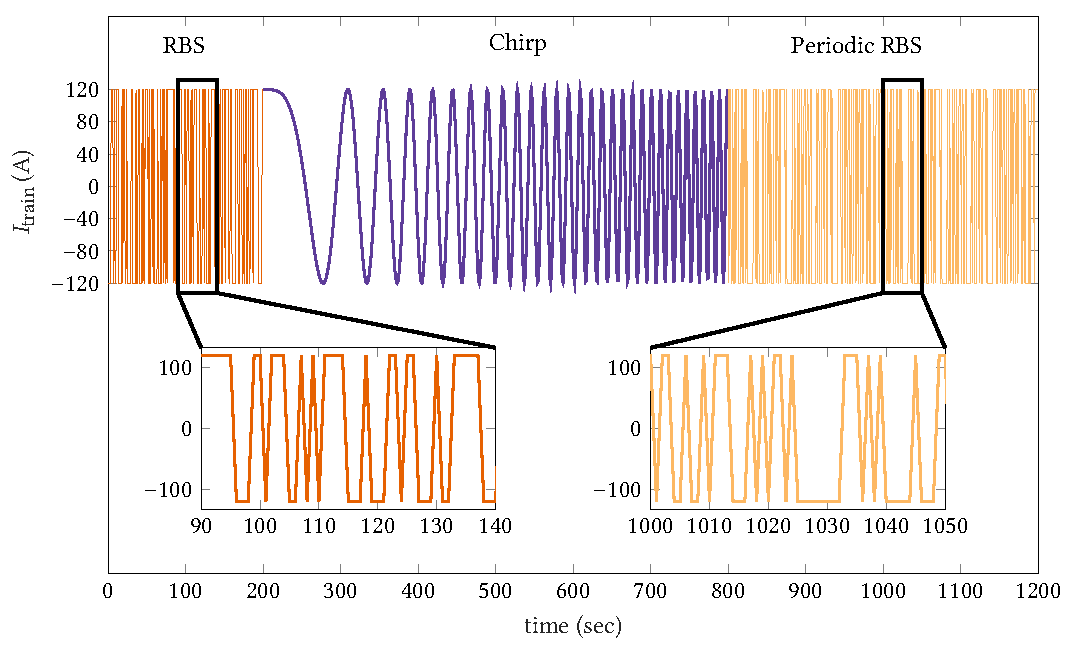
\includegraphics{sysid_train_input.pdf}
    \captionsetup{singlelinecheck=off}
    \caption[Input current profile used as the training set for system
    identification]{Input current profile used as the training set for system
    identification. The sequence consists of
    \begin{enumerate*}[label=\emph{\alph*})] \item a \glsfmtlong{rbs}, \item a
        chirp or swept cosine signal (0--\SI{100}{\milli\hertz}), and \item a periodic \glsfmtlong{rbs} \end{enumerate*} thereby
covering both low and high frequency spectra while incorporating the potential
to excite any periodic modes in the system to be identified.}
    \label{fig:sysidtrainingcurrent}
\end{figure}

\subsection{Validation current profile}

For the  purposes of identification,  the \gls{p2d}  model is considered  as the
true system. First, the current profile from  the training set is applied to the
\gls{p2d} model.  Its simulation results,  in particular the  numerically solved
concentration values  at each spatially  discretised node  in each of  the three
regions per time-step is integrated over the thickness of the respective regions
and multiplied with their respective porosities to obtain the number of moles of
\ch{Li^+} per unit area in each  of the three regions~$Q_{\text{e,}j}$. Only the
quantities  $Q_\text{e,n}$ and  $Q_\text{e,p}$  are chosen  as  the outputs  for
system  identification and  a  transfer  function model  is  fitted  as per  the
evaluation procedure discussed in \cref{sec:actualsysid}.

As with  any classical  curve fitting  (numerical regression)  procedure, system
identification is also  prone to overfitting the training data.  In general, the
`best' transfer  function that identifies the  given system is the  lowest order
model that not  only minimises the training error, but  also minimises the error
on a  previously unseen  validation dataset.  In the  absence of  an independent
validation  dataset,  the  training  error  can be  made  arbitrarily  small  by
increasing the number of poles and zeros of the transfer function models without
any bounds. However,  such a model shall not have  truly identified the dynamics
of the system  and shall not generalise well to  real-world datasets outside the
training realm. Hence, having an  independent validation current profile for the
task at hand is of paramount importance.

For the system identification task at  hand, the characteristic waveforms of the
validation profile were deliberately conjured to be differ vastly from that used
in training the model. The  validation profile consists of the following
sequence
\begin{enumerate}
    \item Periodic \gls{rgs} with 4~periods of \SI{200}{\second} each\quad (0--\SI{799}{\second})
    \item \gls{prbs} for emulating white noise \ie~with a flat power spectra
        across the frequency spectrum\quad (800--\SI{999}{\second})
    \item Multi-sine signal \ie~a signal consisting of sinusoids at
        various fundamental frequencies added together\quad (1000--\SI{1199}{\second})
\end{enumerate}

Overall,  the validation  profile has  been designed  to cover  a wide  range of
frequencies  akin to  the  training  profile, but  differing  completely in  its
time-domain appearance.  The specific  validation current  profile used  in this
system identification is shown in \cref{fig:sysidvalidationcurrent}.

\begin{figure}[!htbp]
    \centering
    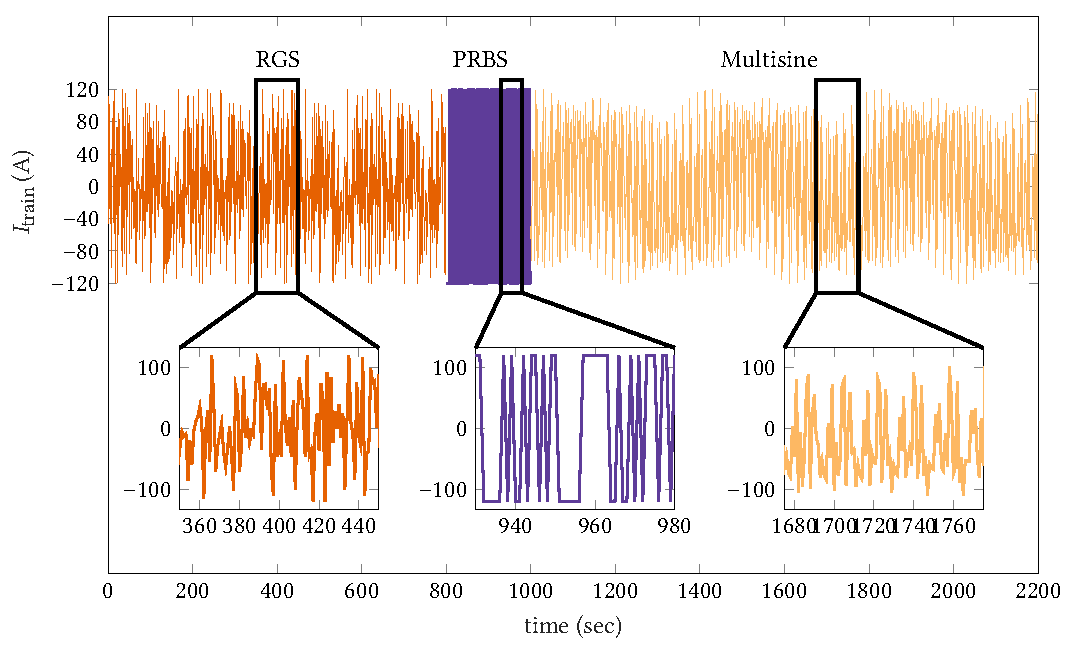
\includegraphics{sysid_validation_input.pdf}
    \captionsetup{singlelinecheck=off}
    \caption[Input current profile used as the validation set for system
    identification]{Input current profile used as the validation set for system
        identification. The sequence consists of
        \begin{enumerate*}[label=\emph{\alph*})]
            \item a \glsfmtlong{rgs},
            \item a \glsfmtlong{prbs}, and
            \item a multisine waveform
        \end{enumerate*}.
        The overall sequence  is intended to emulate the flat  power spectrum of
        white noise (with the \glsfmtshort{prbs}) and excite any poles and zeros
        within~\mbox{3$\sigma$} spread  of the  \glsfmtshort{rgs} mean.  The multisine
        signal is  swept is composed  of sinusoids with  fundamental frequencies
        from \SI{100}{\milli\hertz}  up to the Nyquist  frequency. Its amplitude
        variation  across the  frequency spectrum  increases the  probability to
        capture the  system's modes that  were possibly missed by  the preceding
        two waveforms.
    }%
    \label{fig:sysidvalidationcurrent}
\end{figure}

\textsc{MATLAB} code  that can be used  to generate the training  and validation
input profiles is shown in \cref{codesnippet:trainvalidsysidinput}.

\begin{listing}[!htbp]
\begin{minted}[mathescape,autogobble,bgcolor=mintedbg,escapeinside=||,texcomments=true]{matlab}
% Needs matlab's system identification toolbox
clear; close all; clc; format short g;
warning('off','Ident:dataprocess:idinput7'); % suppress sysid warnings
I_1C  = 60; % Amps
range = 2*[-I_1C I_1C]; % peak-peak swing is $\pm 2\text{C}=\SI{40}{\ampere}$
NumCh = 1; % no of channels (used by sysid toolbox for multichannel id)
Ts    = 1; % sampling interval

%% Random Binary Input Signal (RBS)
N  = 200; % samples per quantum of each waveform
u1 = idinput(N,'rbs',[],range); % 'idinput' from sysid toolbox
%% Chirp Signal (swept cosine)
t_chirp_start = 0;
t_chirp_end   = 3*N*Ts; %
t             = linspace(t_chirp_start,t_chirp_end,3*N);
f0            = 0;
f1            = 1e-1; % $f_1 = \SI{100}{\milli\hertz}$ is the max chirp frequency
u2            = max(range)*chirp(t,f0,t(end),f1)';
%% Periodic Random Binary Input Signal (Periodic RBS)
bin_seq_Period   = N; % seconds
bin_seq_Period_N = ceil(bin_seq_Period/Ts); % samples
bin_NumPeriod    = 2;
u3 = idinput([bin_seq_Period_N,NumCh,bin_NumPeriod],'rbs',[],range);
%% Random Guassian Signal (RGS)
rgs_Period         = N; % seconds
rgs_Period_samples = ceil(rgs_Period/Ts);
rgs_NumPeriod      = 4;
u4 = idinput([rgs_Period_samples,NumCh,rgs_NumPeriod],'rgs',[],range/2);
%% PseudoRandom Binary Signal (PRBS)
prbs_Period         = N; % seconds
prbs_Period_samples = ceil(prbs_Period/Ts);
u5                  = idinput(N,'prbs',[],range);
%% Multisine signal (sum of sines)
samples_per_Period = 2*N;
NumPeriod          = 3;
[u6,freq] = idinput([samples_per_Period 1 NumPeriod],'sine',[],range);

%% Split into training and validation data sets
I_load_train    = [u1;u2;u3];
I_load_validate = [u4;u5;u6];
\end{minted}
\caption{Generation of training and validation input current profiles in
\textsc{MATLAB}}
\label{codesnippet:trainvalidsysidinput}
\end{listing}


\section{Investigation of Linearity and Time Invariance}\label{sec:lticheck}
% -*- root: ../main.tex -*-
%!TEX root = ../main.tex
% this file is called up by main.tex
% content in this file will be fed into the main document
% vim:textwidth=80 fo=cqt


The      transfer     function      identification     techniques      mentioned
in \cref{sec:introblackboxsysid} are  applicable only for \gls{lti}  systems. At
first glance,  this seems to  be overly restrictive  for the system(s)  at hand.
When  considered  as  a  single  macroscopic  entity,  a  lithium  ion  battery,
exhibits  overall non-linear  characteristics,  particularly due  to the  strong
non-linearities in
\begin{enumerate*}[label=\emph{\alph*})]
    \item the Butler-Volmer reaction kinetics (see \cref{eq:butlervolmer}), and
    \item the \glspl{ocp} of the two electrodes (see \cref{eq:lcoUocpPos} and \cref{eq:lcoUocpPos}).
\end{enumerate*}
However,  we are  dealing with  a much  narrower scope  \ie~the  systems under
consideration  are just  the two  sub-system entities  (one per  electrode) that
transform the  applied current at  a particular  time-step to the  overall moles
per  unit area  of  \ch{Li^+}  ions in  the  corresponding  electrode region  of
the  electrolyte at  that  same  instant. Therefore,  it  is  the linearity  and
time-invariance of these \emph{subsystems} that must be investigated.

\subsection{Time-invariance of the electrolyte time-evolution subsystems}\label{subsec:timeinvariance}
A  test  for time-invariance  is  prescribed  in  the  lecture notes  on  system
identification by  Plett~\cite{PlettECE5560_02}. The steps involved  therein are
reproduced here after  being suitably adapted to the notation  of the subsystems
at hand.
\begin{enumerate}
    \item Apply input~${u_1(t) = I(t)}$ to the system and measure the outputs~$Q_{\text{e,n}_1}\!(t)$ and~$Q_{\text{e,p}_1}\!(t)$.
    \item Apply a delayed version of the input by $\tau$~seconds \ie~${u_2(t) = I(t-\tau)}$ to the system and measure the outputs~$Q_{\text{e,n}_2}\!(t)$ and $Q_{\text{e,n}_2}\!(t)$.
    \item If ${Q_{\text{e,n}_2}\!(t) = Q_{\text{e,n}_1}\!(t-\tau)}$ and
        ${Q_{\text{e,p}_2}\!(t) = Q_{\text{e,p}_1}\!(t-\tau)}$ for all possible
        delays~$\tau$, as well as for all choice of input signals~$I(t)$, then the systems are time-invariant.
\end{enumerate}

For the systems at hand, it is  not strictly required to apply this prescriptive
test. Unless a fundamental change in the underlying reaction phenomena/chemistry
occur that  alter the  performance over  time, these systems  can be  treated as
time-invariant. Factors  that induce  time-dependent shift  in the  behaviour of
lithium ion batteries are degradation  phenomena such as thickening of \gls{sei}
layer, dendrite growth or mechanical  fatigue in electrodes which in-turn affect
electrolytic  diffusion and  conductivity. Yet  another cause  of time-dependent
behavioural change  is the drift  in parameter values. However,  these phenomena
are  typically  one or  mode  orders  of  magnitude  slower than  the  \gls{p2d}
dynamics\fxnote{citation needed}. This separation  of time-scales imply that, in
practice they can be decoupled. Therefore, separate models can be identified for
the faster and slower processes. A  suitable model-blending approach can then be
considered  to cover  all processes  across time-scales.  Although the  concepts
developed here for the fast electrolyte dynamics can be suitably adapted to such
slow phenomena, their study  falls outside the scope of this  thesis and is left
as an exercise for  future work. Thus, the overall battery  system, and hence by
extension,  the  two subsystems  considered  are  deemed to  be  time-invariant.
However, in the interest of completeness, this author systematically applied the
aforementioned test procedure with every  combination arising from the choice of
ten time-delay values and the following six current profiles ---
\begin{enumerate*}[label=\emph{\alph*})]
    \item constant current 1C~discharge,
    \item constant current 3C~discharge,
    \item constant current 1C~charge,
    \item \gls{udds} input profile with peak amplitude of~3C,
    \item training profile used in system identification (see \cref{fig:sysidtrainingcurrent}), and
    \item validation profile used in system identification (see \cref{fig:sysidvalidationcurrent}).
\end{enumerate*}
Finally,  these tests  were  repeated for  a choice  of  five different  initial
\glspl{soc}   ---   \SI{90}{\percent},   \SI{70}{\percent},   \SI{50}{\percent},
\SI{30}{\percent}  and \SI{10}{\percent}\footnote{\label{fn:socstart}The  number
of  moles  of  \ch{Li^+} per  unit  area  in  the  electrolyte does  not  depend
on  the  electrode's \glsfmtshort{soc}.  However,  different  starting point  of
\glsfmtshort{soc}s were considered  to have a wide variety in  the length of the
recorded  data until  cut-offs  were hit.  \eg~starting at  \SI{90}{\percent}
\glsfmtshort{soc} could  mean that  for a  current spike  early in  the profile,
upper  cut-off voltage  shall be  hit  sooner leaving  a smaller  set of  logged
simulation data.}.

\begin{figure}[!htbp]
    \centering
    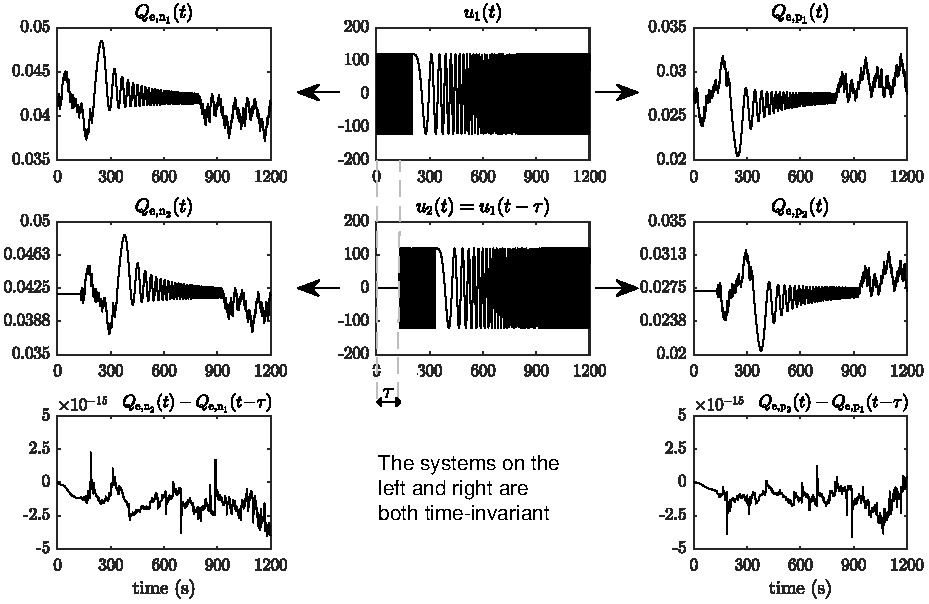
\includegraphics[width=\textwidth]{time_invariance.pdf}
    \caption[Demonstration of time-invariance of~$Q_\text{e,n}(t)$ and
    $Q_\text{e,p}(t)$ subsystems]{Demonstration of time-invariance of the
        subsystems considered. The applied current profile~$u_1(t)$ is the
        system identification training sequence
        from \cref{fig:sysidtrainingcurrent} (top row of the central column).
        The top left plot shows the response $Q_{\text{e,n}_1}\!(t)$, while that
        on the top right shows~$Q_{\text{e,p}_1}\!(t)$. The second row of the
        middle column shows the same input sequence delayed by ${\tau =
        \SI{130}{\second}}$. Application of this current profile $u_2(t) =
        u_1(t-\tau)$ results in the outputs~$Q_{\text{e,n}_2}\!(t)$ and
        $Q_{\text{e,p}_2}\!(t)$ to its left and right respectively. Subtracting
        these from the correspondingly delayed versions of the original outputs
        result in zero residuals, thereby proving time-invariance of these
        subsystems. The jitter shown in the bottom row of plots is
        $\mathcal{O}(10^{-15})$ in magnitude and are due to the numerical
        roundoffs that occur when operating close to the noise floor of the
    machine's floating point units.}%
\label{fig:timeinvariance}
\end{figure}
% The outputs $Q_\text{e,n}$ and $Q_\text{e,p}$ are shown to the left and right of the applied input.

\Cref{fig:timeinvariance}  demonstrates the  time-invariance  of the  subsystems
considered  at  an  initial  \gls{soc} of  \SI{50}{\percent}  for  a  time-delay
of   \SI{130}{\second}   using   the  highly   dynamic   system   identification
training    sequence   that    was   synthesised    by   this    thesis   author
(see \cref{fig:sysidtrainingcurrent}).  The  applied  current  profile~$u_1(t)$
(top row  of the  central column)  produces the  outputs~$Q_{\text{e,n}_1}\!(t)$
and  $Q_{\text{e,p}_1}\!(t)$  shown  in  the   top  left  and  top  right  plots
respectively.  When  the delayed  version  of  this  input sequence  ${u_2(t)  =
u_1(t-\tau)}$ (middle row, middle column) is  applied, it results in the outputs~$Q_{\text{e,n}_2}\!(t)$  and  $Q_{\text{e,p}_2}\!(t)$  to  its  left  and  right
respectively.  Following the  steps  of the  test  procedure, subtracting  these
outputs from the correspondingly delayed versions of their original counterparts
result in  zero residuals, thereby  proving time-invariance of  these subsystems
under these representative test conditions. The residual sequences in the bottom
row of plots are of~$\mathcal{O}(10^{-15})$ and arise due to numerical roundoffs
that occur  when operating close  to the noise  floor of the  machine's floating
point units.

Similar to  the case demonstrated  here, all  tests for time-invariance  for all
permutations of  the chosen operating  conditions passed successfully  \ie~the
delayed  version of  the original  output  signals accurately  matched with  the
responses  to  the corresponding  delayed  input  (down to  machine  precision),
thereby confirming the time-variance of  the subsystems considered in the system
identification problem, which enables us to proceed further.


\subsection{Linearity analysis of the electrolyte time-evolution subsystems}\label{subsec:linearityanalysis}

\subsubsection*{De-biasing of  input signals}

In the analyses of linearity of systems, it is a recommended practice to de-bias
the output and input quantities about their mean operating conditions. The input
signal  in this  case is  the  applied load  current~$I(t)$, which  can be  both
positive  (during discharge)  and  negative  (during charge).  The  mean of  the
training  profile is  \SI{-1.167}{\ampere} and  that of  the validation  profile
is~\SI{-0.3273}{\ampere}. Clearly, the mean values are dependent upon the actual
current profile used. The appropriately de-biased signal \ie~$\widetilde{I}(t) =
I(t) - \bar{I}(t)$  is to be used  for training and validation data  sets in the
system identification procedure. For the purpose  of linearity analysis, it is a
standard practice to simply apply a step change in input (from zero) and measure
the output responses, thereby bypassing the de-biasing requirements.

% Although, in  principle, the strength  of the input  signal does not  affect the
% linearity tests, for  the actual system identification  procedure, the de-biased
% signal must still be persistently exciting as in \cref{sec:persistentexcitation}
% must be

For the output signals, bias  values can be pre-computed analytically and
accounted for.  The overall number  of moles of \ch{Li^+}  per unit area  in any
region within  the cell cannot  be physically  negative. Even though  under high
C-rates,  ion depletion  at localised  spatial  locations (such  as the  current
collectors) is  certainly possible,  the entire thickness  of any  region cannot
become devoid of ions at any point  in time since the cell shall instantaneously
cease  to work.  Thus, for  a typical  well-designed cell  operating within  the
manufacturer prescribed  C-rate limits,  the output signals  under consideration
operate  in  a  small  window  about  their  initial  values.  In  the  author's
simulations, even  at~$\pm$5C, the overall  number of moles of  \ch{Li^+} in any
cell region exhibited  a maximum change of less than  \SI{15}{\percent} from its
initial value. Thus,  the de-biased output variables  for system identification~$\widetilde{Q}_{\text{e,}j}(t)$ can be obtained  by subtracting their respective
initial values~$Q_{\text{e,}j}(0)$ (see \cref{eq:Qeninit} and \cref{eq:Qepinit})
from~$Q_{\text{e,}j}(t)$.
\begin{align}
    \widetilde{Q}_\text{e,n}(t) & = {Q}_\text{e,n}(t) - {Q}_\text{e,n}(0) \\
    \widetilde{Q}_\text{e,p}(t) & = {Q}_\text{e,p}(t) - {Q}_\text{e,p}(0)
\end{align}
which  implies   that  the   transfer  functions  to   be  identified   have  to
be   modified   to   be   $\frac{\widetilde{Q}_\text{e,n}(s)}{\bar{I}(s)}$   and
$\frac{\widetilde{Q}_\text{e,p}(s)}{\bar{I}(s)}$  respectively.  This  does  not
affect  the  time-invariance  proved in \cref{subsec:timeinvariance}  since  the
initial  values~$Q_{\text{e,}j}(0)$  are   merely  constants  and   hence  not
time-dependent.

\subsubsection*{Test for linearity}
Similar     to      the     test      for     time      invariance     described
in \cref{subsec:timeinvariance}, a  test for linearity is  also prescribed in
the lecture notes on  system identification by Plett~\cite{PlettECE5560_02}. The
steps involved therein  are reproduced here after being suitably  adapted to the
notation of the subsystems at hand. This is essentially a recipe for testing the
superposition principle.
\begin{enumerate}
    \item Apply input profile~$I_1(t)$ to the system and obtain outputs~$\widetilde{Q}_{\text{e,n}_1}\!(t)$ and~$\widetilde{Q}_{\text{e,p}_1}\!(t)$.
    \item Apply a different profile~$I_2(t)$ to the system and obtain outputs~$\widetilde{Q}_{\text{e,n}_2}\!(t)$ and~$\widetilde{Q}_{\text{e,n}_2}\!(t)$.
    \item Now apply an input profile~$I_3(t) = \alpha I_1(t) + \beta I_2(t)$ and obtain a corresponding set of outputs~$\widetilde{Q}_{\text{e,n}_3}\!(t)$ and $\widetilde{Q}_{\text{e,n}_3}\!(t)$.
    \item If ${\widetilde{Q}_{\text{e,n}_3}\!(t) = \alpha\,
            \widetilde{Q}_{\text{e,n}_1}\!(t) + \beta \,
            \widetilde{Q}_{\text{e,n}_2}\!(t)}$ and
            ${\widetilde{Q}_{\text{e,p}_3}\!(t) = \alpha\,
                \widetilde{Q}_{\text{e,p}_1}\!(t) + \beta \,
            \widetilde{Q}_{\text{e,p}_2}\!(t)}$ for all possible~$\{\alpha,\beta\}$ as well as for choice of input signals~$\{I_1(t),I_2(t)\}$, then the systems are linear.
\end{enumerate}

As   in   the  time-invariance   test,   the   same   set  of   five   different
initial  \glspl{soc}\textsuperscript{\ref{fn:socstart}}  ---  \SI{90}{\percent},
\SI{70}{\percent},  \SI{50}{\percent}, \SI{30}{\percent}  and \SI{10}{\percent},
was  retained for  these linearity  tests. For  each test  run, a  pseudo-random
number generator  was used to select  the values of~$\{\alpha,\beta\}$  from the
set  of  real numbers~$\mathbb{R}$  (not  restricted  to  the set  of  integers~$\mathbb{Z}$) in  the closed  interval spanning~$[-1.25,1.25]$.  Negative values
are acceptable for  both the scaling coefficients since  the resulting composite
input~$I_3(t)$ can be either positive or negative. The composite signal $I_3(t)$
was obtained by taking a random combination  of any two of the following current
profiles ---
\begin{enumerate*}[label=\emph{\alph*})]
    \item step input with a constant current 1C~discharge,
    \item step input with a constant current discharge at~C/5,
    \item step input with a constant current 1C~charge,
    \item step input with a constant current charge at~C/5,
    % \item de-biased training profile used in system identification (see \cref{fig:sysidtrainingcurrent}), and
    % \item de-biased validation profile used in system identification (see \cref{fig:sysidvalidationcurrent}).
\end{enumerate*}

The   scaling   factors~$\alpha$   and    $\beta$   were   restricted   to   the
range~$[-1.25,1.25]$ in  consideration of limiting  the peak applied  current to
within a~\pm 3C window --- the operating condition for most \glspl{bev}, so that
the isothermal  assumption for the model  shall remain valid. This  peak current
corner case occurs when the pseudo-random generator chooses both scaling factors
at the selected range's limits for the 1C~constant current discharge or charging
cases. The limited range  of the scaling factors are also  motivated by the fact
that  most real-world  systems remain  linear  only within  a certain  operating
window. In  particular, care must be  taken to ensure that  the cell's \gls{soc}
during the  linearity test remains  within its  physical limits for  any initial
\gls{soc}. Furthermore, localised  saturation or depletion of  ions for extended
durations must be avoided. Hence it can be concluded that, with the chosen range
for the scaling factors, if the two subsystems under consideration remain linear
everywhere  below a  peak current  of~\pm 3C  in the  isothermal case,  then the
linearity  tests are  considered as  passed.  Future extensions  to undertake  a
temperature-dependent  system  identification  exercise can  potentially  use  a
first-order Taylor  expansion about this  operating window. The  discussion thus
far  has fully  established  all  the conditions  for  conducting  the test  for
linearity.

\begin{figure}[!htbp]
    \centering
    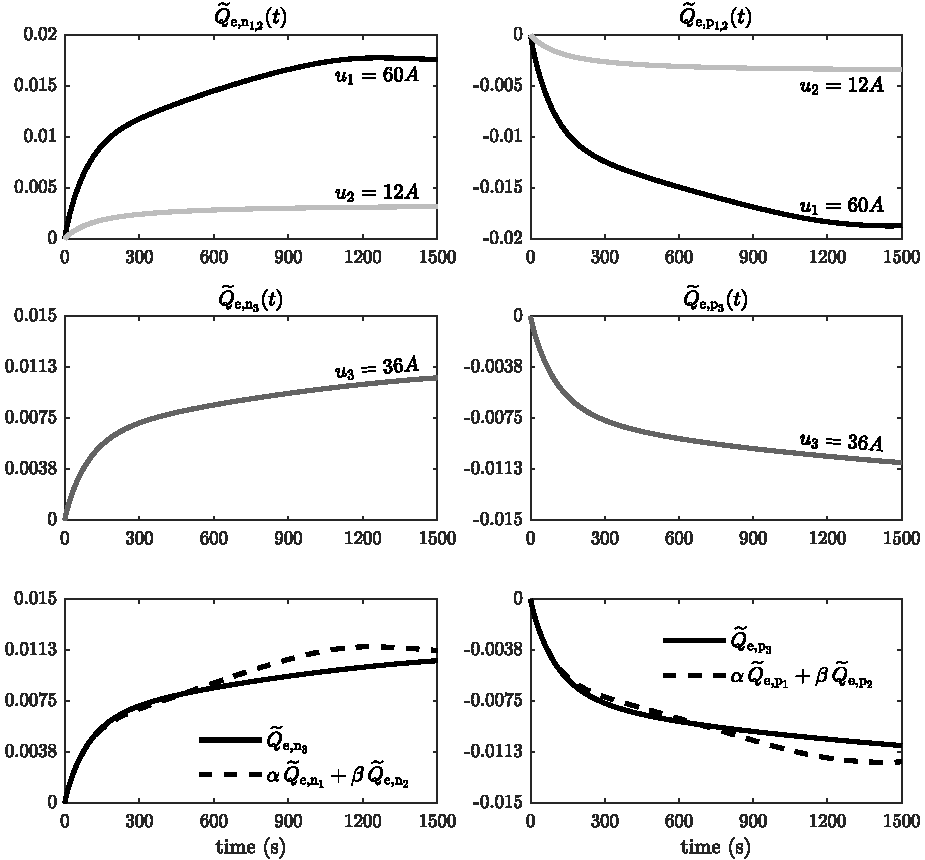
\includegraphics[width=\textwidth]{linearity_proof}
    \caption[Illustration of linearity test for the
    \protect{$\widetilde{Q}_{\text{e,n}}$} and
    \protect{$\widetilde{Q}_{\text{e,p}}$} subsystems]{Illustration of one
        instance of linearity tests for the subsystems under consideration. For
        this visualisation, constant current inputs are used throughout. The top
        row of plots shows $\widetilde{Q}_{\text{e,n}}$ and
        $\widetilde{Q}_{\text{e,p}}$ for two step inputs~${I_1(t) =
        \SI{60}{\ampere}}$ and $I_2(t) = \SI{12}{\ampere}$ \ie~discharge with~1C and C/5~currents respectively. The second row of plots shows
        $\widetilde{Q}_{\text{e,n}_3}$ and $\widetilde{Q}_{\text{e,p}_3}$  for
        ${I_3 = \SI{36}{\ampere}}$, where $I_3 = \alpha I_1 + \beta I_2$ with~${(\alpha,\beta) = (1,-2)}$. The last row of plots overlays these
        quantities with the manually computed linear combination of their two
        preceding responses. Had these sequences overlapped exactly, the systems
        would have been exactly linear. Despite exhibiting deviations over the
        considered horizon, the transient responses in both electrode regions do
        follow the superposition principle. Even past the transient, maximum
        error in both cases is an order of magnitude lower than the individual
        outputs. Hence, the two systems are deemed to be \emph{approximately}
        linear.
    }%
    \label{fig:linearity}
\end{figure}

\Cref{fig:linearity}  illustrates  one  instance  of a  linearity  test  wherein
constant  currents  and  integer  scaling  factors are  used  for  the  sake  of
illustration.  The  plots   in  the  left  column  deal   with  the  electrolyte
time-evolution  subsystem  in  the  negative electrode  region.  Similarly,  the
plots  in  the  right  column  deal with  the  corresponding  subsystem  in  the
positive electrode region.  A discharge current of~1C  \ie~\SI{60}{\ampere} is
first  applied  and  the  corresponding  outputs~$\widetilde{Q}_{\text{e,n}_1}$
and   $\widetilde{Q}_{\text{e,p}_1}$  are   obtained.   Secondly,  a   discharge
current   of   C/5   \ie~is    applied   and   the   corresponding   outputs~$\widetilde{Q}_{\text{e,n}_2}$ and  $\widetilde{Q}_{\text{e,p}_2}$ are obtained.
These set of responses are plotted  in the top row of \cref{fig:linearity}. Now,
a  third  value  of  input  current~$I_3$,  computed  as  a  linear  combination
of  the  previous  input  currents  \ie~${I_3 =  \alpha  I_1  +  \beta  I_2  }$
is  applied.  For  illustrative  purposes, the  integer  set  ${(\alpha,\beta)  =
    (1,-2)}$  was  chosen  for  the   scaling  coefficients,  which  implies  ${I_3  =
\SI{12}{\ampere}}$. The corresponding  outputs~$\widetilde{Q}_{\text{e,n}_3}$ and
$\widetilde{Q}_{\text{e,p}_3}$ are  plotted in the  middle row. As per  the test
for linearity,  if these signals are  equal to the signal  generated by manually
computing the linear  combination of the preceding two outputs,  then the system
is linear.

The   plots   in  the   third   row   show  $\widetilde{Q}_{\text{e,n}_3}$   and
$\widetilde{Q}_{\text{e,p}_3}$ overlaid with their respective linear combination
signals. In  the case  of the  subsystem in the  negative electrode  region, the
transient performance matches  precisely until \approx\SI{450}{\second}, whereas
that in the positive electrode region exhibits a good matching for approximately
the  first~\SI{250}{\second}.  However,  for  the  horizon  considered  the  two
overlaid plots do not overlap exactly.  Hence, the systems are not truly linear.
However,  the  exhibited  behaviour  is  quite  close  to  linearity,  with  the
maximum  absolute error  in each  region,  even outside  the initial  transient,
being~$\mathcal{O}(10^{-4})$ --- an order of magnitude lower than its individual
components.  This behaviour  was exhibited  for all  test instances  considered.
Considering  that for  dynamic  simulation runs,  the  transient performance  is
paramount  to  the good  performance  of  the  model,  in conjunction  with  the
aforementioned  low error  metric,  these  subsystems can  be  considered to  be
\emph{approximately} linear.

Based  on  the  analysis  presented   here,  \gls{lti}  behaviour  for  the  two
subsystems is  assumed, which facilitates  in proceeding with the  actual system
identification procedure.




\section[Transfer Function Identification Procedure]{Transfer Function Identification Procedure\footnote{The early stages of this section presents this author's digested summary of the theoretical framework adapted from a subset of content from the lecture notes on system identification by Plett~\cite{PlettECE5560_02,PlettECE5560_03,PlettECE5560_04}.}}\label{sec:actualsysid}
% -*- root: ../../main.tex -*-
%!TEX root = ../../main.tex
% this file is called up by main.tex
% content in this file will be fed into the main document
% vim:textwidth=80 fo=cqt

\subsection{The transfer operator and its model form}
In a classical system identification  task, the discrete-time transfer functions
for the systems  under consideration need to be  determined. These discrete-time
transfer functions are  based on Z-transforms in the  frequency domain. However,
for the purpose of working in time-domain, an analogous linear operator~$q$ that
performs a  forward shift on  its input \ie~$  {q u[k] \longmapsto  u[k+1]} $.
Similarly, applying the  backward shift operator~$ q^{-1} $  on the input yields
its value at the previous time-step \ie~$ {q^{-1} u[k] \longmapsto u[k-1]}$.


In a generic  \gls{lti} system wherein measurements are corrupted  by noise, The
system  dynamics are  represented by  the transfer  operator~$G(q)$\footnote{The
term  transfer operator  in the  time domain  mathematically corresponds  to the
term  transfer  function  in  the  frequency  domain.  Mathematically,~${G(q)  =
G(z)\bigr\rvert_{\mathrlap{z=q}}}$.}  that  acts  on the  applied  input~$u[k]$,
whereas the  noise dynamics are  represented by the  disturbance operator~$H(q)$
that acts to filter (or shape) an assumed white noise input~$e[k]$.

Assuming linearity and time-invariance throughout, the overall output can be
written as the linear combination
\begin{equation}\label{eq:outputwithsysandnoise}
    % \SwapAboveDisplaySkip
    y[k] = G(q)u[k] + H(q)e[k]
\end{equation}
where ${G(q) = \frac{B(q)}{A(q)}}$ and ${H(q) = \frac{C(q)}{D(q)}}$ are the transfer
operators describing the dynamics of the system and disturbance respectively.

${A(q), B(q), C(q) \text{ and } D(q)}$ are rational polynomials in~$q$. The two transfer
operators~$G(q)$ and $H(q)$ can be represented by
\begin{align}
    G(q) &= q^{-n_k}\frac{b_1q^{-1} + \dots  + b_{n_b}q^{-{n_b}}}{1 + a_1q^{-1} + \dots  + a_{n_a}q^{-{n_a}}} \\
    H(q) &= q^{-n_l}\frac{c_1q^{-1} + \dots  + c_{n_c}q^{-{n_c}}}{1 + d_1q^{-1} + \dots  + d_{n_d}q^{-{n_d}}}
\end{align}
where ${(n_k,n_l)}$ represent  the number of transport  delay samples, $(n_b,n_c)$
the number  of feedforward coefficients  and ${(n_a,n_d)}$, the number  of feedback
coefficients in $G(q)$ and $H(q)$ respectively.


In  this  system  identification  task  at hand,  the  output  measurements  are
collected from a  \emph{noise-free} simulation of the \gls{p2d}  model \ie~the
disturbance transfer operator in \cref{eq:outputwithsysandnoise} is zero
\begin{align}
    y[k] &= G(q)u[k] + \cancelto{0}{H(q)}e[k]
\shortintertext{Hence, the time-domain output  reduces  to}
y[k] &= G(q)u[k] \label{eq:outputwithsysonly}
\end{align}

Thus, the system identification task becomes one that of estimating
\begin{enumerate}
    \item The number of transport delay samples~$n_k$.
    \item The number of feedforward coefficients (zeros)~$n_b$.
    \item The zeros themselves~${b_1, b_2, \dots b_{n_b}}$.
    \item The number of feedback coefficients (poles)~$n_a$.
    \item The pole locations~${a_1, a_2 \dots a_{n_a}}$.
\end{enumerate}
for  each  of  the  two  transfer operators~$G_1(q)$  and  $G_2(q)$  \ie~the
electrolyte  time-evolution subsystems  in the  negative and  positive electrode
region respectively.

\subsection{Estimation of transport delay}

The transport delay~$n_k$ can be estimated visually by inspecting the step
response of the systems under consideration.

In \cref{fig:linearity},   step  inputs   of   ${I_1   =  \SI{60}{\ampere},   I_2
=    \SI{12}{\ampere},}$   and    ${I_3   =    \SI{36}{\ampere}}$   were    applied
to    the   two    subsystems.    Inspecting   closely    all   the    responses
\ie~$\widetilde{Q}_{\text{e,n}_1},    \widetilde{Q}_{\text{e,n}_2}   $   and
$\widetilde{Q}_{\text{e,n}_3}$    in    the     negative    electrode    region,
and    $\widetilde{Q}_{\text{e,p}_1},    \widetilde{Q}_{\text{e,p}_2}   $    and
$\widetilde{Q}_{\text{e,p}_3}$  in the  positive electrode  region, it  is clear
that all these outputs start exactly at  zero. Therefore, there is no delay term
to be considered for the transfer operators \ie~${n_k = 0}$ for both subsystems.

\subsection{Choice of model structure}\label{subsec:modelstrucchoice}

Among      the      transfer-function       model      structures      mentioned
in \cref{subsec:parametric}, the \gls{arx} model  structure is too simplistic to
consider. Despite  the fact that  its numerical computation involves  only basic
linear algebra operations,  that can be efficiently handled  on modern computing
systems, it  is considered to produce  poor estimates of the  system's poles and
zeros. In the absence of contributions from the noise-term, the all-encompassing
model structure used by the Box-Jenkins approach is deemed to be unnecessary for
the  problem  at hand.  Therefore,  the  two  model structures  considered  were
\gls{armax} and \gls{oe} for the coefficient determination.

\subsection{Starting guesses for coefficient orders}\label{subsec:initguesscoefforder}

At first, the training profile of \cref{fig:sysidtrainingcurrent} is
de-biased (through mean removal) and applied as the input current profile in a \gls{p2d}
simulation. The outputs of this simulation are suitably post-processed as per
the following sequence of steps.
\begin{enumerate}
    \item The concentrations solved at various node locations within each
        electrode are numerically integrated over the corresponding electrode
        thicknesses using trapezoidal rule.
    \item The resulting integral value is multiplied with the porosity of the
        corresponding electrode region to obtain $Q_{\text{e,n}_\text{train}}(t)$ and~$Q_{\text{e,p}_\text{train}}(t)$.
    \item These quantities are then de-biased by subtracting their initial
        values to obtain $\widetilde{Q}_{\text{e,n}_\text{train}}(t)$ and~$\widetilde{Q}_{\text{e,p}_\text{train}}(t)$.
\end{enumerate}

The        same        procedure        is        repeated        for        the
validation       current      profile       of \cref{fig:sysidvalidationcurrent}
to         obtain         $\widetilde{Q}_{\text{e,n}_\text{val}}(t)$         and~$\widetilde{Q}_{\text{e,n}_\text{val}}(t)$.  These data  sets are  used for  all
subsequent sub-tasks involved in this system identification exercise.

In  order to  reduce  the search  window for  the  coefficient determination  in
the  parametric transfer  function methods,  the hand-estimation  of coefficient
order  through non-parametric  methods may  be performed.  This coarse  estimate
can  act as  a  feeder to  help  in  the faster  convergence  of the  non-linear
optimisation algorithms  used in the parametric  methods. In this case,  a basic
spectral analysis  using a Hanning  window implemented using the  MATLAB command
\texttt{spa.m} is applied to the time-domain data to transform it into frequency
response data.

\begin{figure}[!htbp]
    \centering
    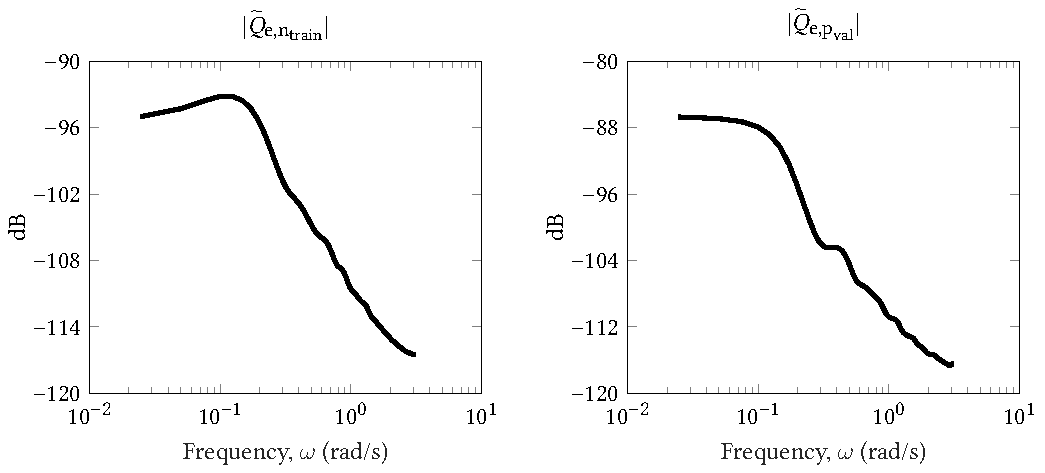
\includegraphics[width=\textwidth]{chapters/sys_id/figures/bode_mag.pdf}
    \caption[Bode magnitude plots of the electrolyte time-evolution sub-systems]{%
        Bode magnitude  plots showing the  estimated frequency response  for the
        two  subsystems under  consideration.  The frequency  response data  was
        obtained  through a spectral  analysis \ie~by computing  the ratios  of
        spectra of the de-biased input  and output sequences. The sequences were
        smoothed using a Hanning window before computing the ratio.
    }%
    \label{fig:initialbodemag}
\end{figure}

\Cref{fig:initialbodemag}  shows  the  Bode  magnitude  plot  of  the  frequency
response for
\begin{enumerate*}[label=\emph{\alph*})]
    \item the training set in the negative electrode region, and
    \item the validation set in the positive electrode region.
\end{enumerate*}
In the  plots, a broad  combination of  the two data  sets in the  two electrode
region  is  depicted  to  achieve  a  compact  representation  of  all  possible
permutations and to avoid redundancies by plotting visually similar information.
It is important to note that these Bode diagrams obtained by such non-parametric
methods only represent  a crude approximation of the  physical dynamics intended
to help in initial estimates of the system behaviour.

Some preliminary understanding of the  various characteristics of the system can
be gleaned from these Bode diagrams.  The first visually striking feature is the
similarity  in the  approximate frequency  characteristics in  the negative  and
positive electrode  regions, even when  excited by completely different  data in
the time domain. This confirms the author's assumptions of equal `complexity' in
the symbolic  regression search discussed in \cref{subsec:symbolicreg}.  This is
also  congruent with  the physical  behaviour of  the electrolyte  in these  two
regions.

\subsubsection*{Finite DC gain}
By visual  extension of  the frequency responses  towards lower  frequencies, it
is  clear  that  the  DC  gains  of  both  the  systems  are  finite  and  below
unity.  This  behaviour  can  clearly  be  seen  in  the  time-domain  responses
of \cref{fig:linearity}.  For  the plotted  time-horizon,  this  effect is  most
visible for the case of the \SI{12}{\ampere} constant current input, wherein the
responses of both regions settle to a finite value after an initial transient.

There is \approx\SI{10}{\decibel} variability in  the low frequency gain between
the two Bode  plots in \cref{fig:initialbodemag}. This can be  attributed to the
following  factors. A  compromise with  the spectral  estimation method  is that
using a higher number of frequency bins  results in lower resolution per bin and
vice-versa. By  varying the number  of frequency bins  and focusing on  the low
frequency range, the resolution of the DC  gain can be improved. The rest of the
variability can  be attributed to the  fact that the training  and test profiles
behave differently and do not excite the same dynamics. In particular, the swept
frequency cosine (chirp) signal in the training set was specifically designed to
draw out  the low frequency  dynamics with a  high fidelity. Finally,  the small
range of variation in the DC gain could also be due to the intrinsic small-scale
variations of  the electrolyte  behaviour in  these two  regions. Although  on a
macroscopic frequency scale the two regions behave similarly, the differences in
electrode thicknesses and porosities could contribute to the small difference in
the  DC gain.  This  helps  to confirm  that  two \emph{non-identical}  transfer
functions are being sought for --- one for each electrode region.

Finally, the finiteness  of the DC gain  helps to narrow down  the search window
for the parametric model structures. In particular, this fact indicates that the
model structures to be trialled must not  have any integrator terms (or poles at
the origin of the complex plane).

\subsubsection*{Resonance and model order}

First  order  transfer   functions  do  not  exhibit   characteristic  peaks  or
resonances  in  their  frequency  responses.  However,  for  the  Bode  plot  on
the   left   of \cref{fig:initialbodemag},   a   pronounced   resonance   around
\SI{0.15}{\radian\per\second} is observable. This has  an enormous impact --- it
presents  an important  clue  that the  first  order time-evolution  \glspl{ode}
of \cref{eq:negliionmolesquadratic}   and \cref{eq:posliionmolesquadratic}   are
inadequate to represent the system dynamics.

An apparent  contradiction to  the first-order inadequacy  claim stems  from the
Bode plot  on the  right hand side  in \cref{fig:initialbodemag}. In  this case,
there are no resonances in the  magnitude response indicating that a first order
model description is sufficient. However, a vital aspect to be noted here is the
nature of the  validation current profile when compared to  that of the training
current profile.  The coarse  frequency response data  obtained by  the spectral
method is sensitive to the actual  input sequence employed. From systems theory,
the  resonances at  a frequency  occur  due to  the presence  of lightly  damped
complex conjugate poles at that frequency. The periodic \gls{rgs} was explicitly
designed in the  training set and is  however absent in the  validation set. The
unique characteristics  of the validation  set and its influence  on coefficient
order is discussed next.

As per  the arguments presented  in the  preceding discussions, there  exists an
implicit constraint that  the behaviour of the time-evolution  subsystems in the
two electrode  regions are  expected to be  of similar  `complexity'. Therefore,
based  on the  presence of  the resonance  in the  Bode magnitude  plot for  the
response to  training profile  in the  negative electrode region,  it has  to be
concluded that the two subsystems are \emph{at-least} of second order.

\subsubsection*{Estimation of number of poles and zeros}

The  high-frequency  roll-off  in  the   slopes  of  the  Bode  magnitude  plots
in  \cref{fig:initialbodemag}  provide clues  on  the  number  of poles  in  the
system.  The  corner frequency~$\omega_\text{c}$  in  both  cases appear  to  be
around~\SI{0.15}{\radian\per\second}. The  high-frequency slope of  both systems
is \approx\SI{20}{\decibel}  per decade, which  implies that they  have at-least
one more  pole than  the number  of zeros  if using  a continuous  time transfer
function. For  the corresponding z-domain  transfer function, this  implies that
$n_a \ge n_b$.

In the  aspect of estimating the  number and locations of  zeros, the validation
profile outshines  the training profile. While  the Bode plot obtained  with the
training profile  does not indicate  the presence of  zeros in the  systems, the
plateau in \SIrange{0.3}{0.4}{\hertz} range for  the Bode plot of the validation
profile clearly contradicts this. Once again, hypothesising that the two systems
(in the two electrode regions)  have fundamentally identical behaviour with only
small differences owing  to differences in their parameter  values, there exists
at-least one zero in these  continuous-time systems around this frequency range.
The discrete-time discretisation process adds an additional zero to the system.

Based on this preliminary  analysis, the estimates are $n_k = 0,  n_b \ge 2, n_a
\ge 3$.  Only asymptotic approximations  to corner frequencies can  be estimated
from the  Bode plots. Furthermore, the  estimated locations are not  used in the
parametric system identification algorithms and  is of much less importance than
the  model order  estimates.  With this  initial  understanding, the  parametric
system identification procedure is carried out.

\subsection{Refinement of coefficient orders using deterministic criteria}\label{subsec:refinementofcoefforder}

The initial estimate  of coefficient orders in \cref{subsec:initguesscoefforder}
was performed  based only on  a visual inspection  of the Bode  magnitude plots.
Owing to  the fact that  the frequency  response data is  the result of  a crude
ratio of  spectra, there is a  high probability of missing  vital information on
the number and locations of poles and zeros. Hence only a lower bound on the
coefficient orders are available until this point. Next, a set of deterministic
criteria is used to widen and refine the coefficient order range.


Although   the   \gls{arx}   structure   is  deemed   to   be   too   simplistic
(see \cref{subsec:modelstrucchoice}), owing to the fact that only linear algebra
operations are involved, as opposed  to numerical optimisation routines employed
in the  \gls{oe}, \gls{armax} and Box-Jenkins  structures, certain deterministic
criteria for  coefficient order  selection can  be incorporated  for coefficient
order selection.
This  can serve  as  a  refinement  of  the
initial number of  coefficients guessed from the Bode  magnitude plots discussed
in.

For any model structure used, its error can be defined as
\begin{align}
    % \SwapAboveDisplaySkip
    \varepsilon[k]      & = y[k] - \hat{y}_\text{m}[k] \label{eq:sysiderroronlyk}\\
    \shortintertext{where $y[k]$ are true measurements and}
    \hat{y}_\text{m}[k] & = G(q)u[k] \tag{\cref{eq:outputwithsysonly} revisited}
\end{align}
are the model outputs obtained by the assumed transfer operator~$G(q)$ (which is
to be determined).

The  number of  numerator  and denominator  coefficients in  $G(q)$  as well  as
their  values are  to  be determined.  This  set of  unknowns  can be  collected
into a  parameter vector~$\theta$.  Thus, as per  \cref{eq:sysiderroronlyk}, the
error  sequence  is  parametrised  by  $\theta$, and  its  notation  is  amended
to~$\varepsilon[k;\theta]$.

For  an  input-output  data  set  consisting of  $N$~samples,  a  generic  cost
function that may  be applied for all the four  model structures \viz{\gls{arx},
\gls{armax}, \gls{oe} and Box-Jenkins} is
\begin{align}
    V_N(\theta)  & = \sum_{k=1}^N L\left(\varepsilon\left[k;\theta\right]\right)
\shortintertext{where $L(\cdot)$ is a postive-valued scalar loss function.}
\intertext{In a typical system identification task, the sum of squares of the error sequence is  used as the typical loss function, thereby yielding}
    V_N(\theta)  & = \sum_{k=1}^N \varepsilon^2[k;\theta]\label{eq:nonlincostfcnsysid}
    \shortintertext{The vector~$\hat{\theta}$ that minimises this cost function is desired}
    \hat{\theta} & = \text{arg}\,\underset{\theta}{\text{min}} V_N(\theta)
\end{align}

For  the \gls{arx}  model structure, \cref{eq:nonlincostfcnsysid}  reduces to  a
standard quadratic optimisation  problem which may be  solved analytically using
least  squares  linear  algebra.  However,  for  robustness  against  estimation
bias,  instead of  the  standard \gls{ols}  estimates,  the \gls{iv}  estimation
method~\cite{Ljung1999} was used  for this model order  selection task. Applying
this to  the \gls{arx} model  structure, two deterministic model  order criteria
have been defined ---
\begin{enumerate*}[label=\emph{\alph*})]
    \item \gls{aic}, and
    \item \gls{mdl}~\cite{Ljung1999}.
\end{enumerate*}

In  the \gls{aic},  the  optimal  number of  parameters~$\hat{d}$ in  $\theta$
is  obtained   by  minimising   the  modified   log  likelihood   cost  function
\begin{equation}
    V_{N,\text{mod}}(\theta) =  \ln V_N(\theta)  + \frac{2  d}{N}, \quad N \gg d
\end{equation}
In the \gls{mdl} criterion, this cost function is modified to
\begin{equation}
    V_{N,\text{mod}}(\theta) =  V_N(\theta)\left(1 + \frac{d\, \ln N}{N}  \right)
\end{equation}

For the two subsystems at hand, both  criteria converged to the same choices for
the coefficient orders,  yielding ${n_a = 4,  n_b = 4}$ and~${n_k  = 0}$. Therefore,
these values  were used as the  starting points for the  non-linear optimisation
algorithms  used in  determining  the  exact pole  and  zero  locations for  the
discrete-time transfer functions which is described next.

\subsection{Final transfer function coefficients --- Nonlinear optimisation}

For         the         \gls{armax}        and         Box-Jenkins         model
structures, \cref{eq:nonlincostfcnsysid} results  in a non-linear  cost function
which  is  minimised iteratively  using  quasi-Newton  approaches. The  theoretical
foundation  of  standard non-linear  optimisation  methods  such as  L-BFGS  and
Levenberg-Marquardt are  well established whose  detailed explanation is  out of
the scope of this thesis. Although state of the art methods are not covered, the
interested reader  may consult the  textbook by Scales~\cite{Scales1985}  for an
introductory overview of this topic.

The  final  model structures  (for  both  the  positive electrode  and  negative
electrode time-evolution subsystems) in the z-domain are given by
\begin{equation}
    G(z) = \frac{b_1z^{-1} + \dots + b_{n_b}z^{-{n_b}}}{1 + a_1z^{-1} + \dots + a_{n_a}z^{-{n_a}}}\label{eq:genericZtf}
\end{equation}
wherein the coefficients in the numerator and denominator are to be determined.

The  number of  coefficients obtained  from \cref{subsec:refinementofcoefforder}
was  used as  the initial  guess for  the coefficient  orders in  the non-linear
optimisation.  For  the  initial  guesses   for  the  numerical  values  of  the
coefficients~$(a_1, a_2,  \dots a_{n_a})$ and ${(b_1, b_2, \dots  , b_{n_b} )}$, a
randomised  multi-start  algorithm was  used.  For  the two  transfer  functions
identified, no distinction is made  between whether the \gls{armax} structure or
Box-Jenkins structure was  used to arrive at the coefficients.  Since the output
magnitudes of~$\widetilde{Q}_{\text{e,n}}$  and $\widetilde{Q}_{\text{e,p}}$ are
of~$\mathcal{O}{10^{-3}}$,  a  constant  scaling   factor  of~${k  =  1000}$  is
used  to  bring the  order  of  magnitude of  output  data  values to  unity.  A
well-chosen  scaling factor  is often  vital  to the  convergence of  non-linear
optimisation algorithms.  Since the system  is linear, this constant  gain shall
not fundamentally change the dynamics of the  system and can be accounted for by
using the reciprocal  scaling factor of~0.001 in  numerical implementations. The
identification procedure  was carried  out using MATLAB's  System Identification
Toolbox~\cite{matlabsysidtool}.

% -*- root: ../main.tex -*-
%!TEX root = ../main.tex

\begin{table}[!htbp]
    \begingroup
    \sisetup{group-digits=false}
    \centering
    \caption[A sample of system identification results for $\widetilde{Q}_\text{e,n}$]{A sample of results showing four discrete-time transfer functions identified for the electrolyte time-evolution subsystem in the negative electrode region. Only those models that yielded similar errors (within \SI{0.5}{\percent}) across both input datasets were retained.  The fourth order model from case C (shaded in grey) performed the best across  both training and validation profiles and is chosen as the final model.}
    \label{tbl:sysidnegcases}
    \begin{tabular*}{\textwidth}{@{} c   S[table-format=1.4] S[table-format=1.4] S[table-format=1.4] S[table-format=1.4]  S[table-format=1.4,table-column-width=0.95cm] S[table-format=1.4,table-column-width=0.95cm] S[table-format=1.4,table-column-width=0.95cm] S[table-format=1.4,table-column-width=0.95cm] S[table-format=2.2] S[table-format=2.2] @{}}\toprule
        \multirow{2}[2]{*}{\footnotesize Case} & \multicolumn{4}{c}{\footnotesize Numerator} & \multicolumn{4}{c}{\footnotesize Denominator} &  {\multirow{2}[2]{*}{\footnotesize \makecell{Training \\accuracy\\(\%)}}} & {\multirow{2}[2]{*}{\footnotesize \makecell{Validation\\accuracy\\(\%)}}}\\
        \cmidrule(lr){2-5} \cmidrule(lr){6-9}
        {} & \multicolumn{1}{c}{$b_1$}  & \multicolumn{1}{c}{$b_2$}   & \multicolumn{1}{c}{$b_3$}  & \multicolumn{1}{c}{$b_4$}   & \multicolumn{1}{c}{$a_1$} & \multicolumn{1}{c}{$a_2$} & \multicolumn{1}{c}{$a_3$} & \multicolumn{1}{c}{$a_4$} \\
        \midrule
        A & 0.0026 & -0.0025 & {}      & {}      & -1.922 & 0.923  & {}     & {}    & 95.11 & 95.13 \\
        B & 0.0028 & -0.0052 & 0.0025  & {}      & -2.833 & 2.669  & -0.836 & {}    & 99.14 & 98.54 \\
        \Rowcolor{cbrewerintergray}
        C & 0.0028 & -0.0075 & 0.0066  & -0.0019 & -3.577 & 4.767  & -2.801 & 0.612 & 99.73 & 99.28 \\
        D & 0.0026 & 0.0026  & -0.0024 & -0.0024 & 0.060  & -1.906 & -0.058 & 0.907 & 95.12 & 95.14 \\
        \bottomrule
    \end{tabular*}
    \endgroup
\end{table}


\Cref{tbl:sysidnegcases}   shows   the   results  obtained   by   applying   the
aforementioned   non-linear  identification   routines  to   the  time-evolution
subsystems in the negative electrode region. The coefficient orders tried in the
system identification  procedure were informed  by the inferences from  the bode
magnitude plots as well as that obtained by applying the deterministic \gls{aic}
and \gls{mdl}  criteria. Only those  models that yielded similar  errors (within
\SI{0.5}{\percent}) across both input datasets were retained.

As  discussed  in \cref{subsec:initguesscoefforder},   a  first  order  transfer
function cannot capture all the  dynamics of the subsystems under consideration.
Therefore, the lowest order tried in  the identification procedure was two (case
A in \cref{tbl:sysidnegcases}).  As higher order  models were tried,  the system
accuracy improves steadily as  seen in cases B and C. However  in order to avoid
overfitting, the  \emph{lowest} order  model that  produces the  highest matched
accuracy across both training and validation profiles must be chosen.

Case D illustrates  the importance of the initial values  used in the non-linear
optimisation algorithms.  Despite using an  identical number of  coefficients as
case C,  the optimisation algorithm  converges to  a radically different  set of
zeros  and  poles  resulting  in  a  percentage  error  comparable  to  that  of
the  simple second  order  case. The  fourth  order model  from  case C  (shaded
grey  in \cref{tbl:sysidnegcases}) performs  the best  across both  training and
validation profiles and  is chosen as the final model.  The number of numerators
and  denominators match  exactly that  predicted by  the deterministic  criteria
given in \cref{subsec:refinementofcoefforder}. A similar selection procedure was
applied  for  the  identification  of the  transfer  function  corresponding  to
$\widetilde{Q}_{\text{e,p}}$ in the positive electrode region.

The final identified transfer functions (for the scaled output) are
\begin{align}
    \frac{\widetilde{Q}_{\text{e,n}}(z)}{\widetilde{I}(z)} & = \frac{0.002842 z^{-1} - 0.00753 z^{-2} + 0.006595 z^{-3} - 0.001906 z^{-4}}{1 - 3.577 z^{-1} + 4.767 z^{-2} - 2.801 z^{-3} + 0.6118 z^{-4}} \label{eq:finaldisctfneg}\\
    \frac{\widetilde{Q}_{\text{e,p}}(z)}{\widetilde{I}(z)} & = \frac{-0.002809 z^{-1} + 0.007139 z^{-2} - 0.005944 z^{-3} + 0.001614 z^{-4}}{1 - 3.464 z^{-1} + 4.444 z^{-2} - 2.495 z^{-3} + 0.515 z^{-4}}\label{eq:finaldisctfpos}
\end{align}

\begin{figure}[!htbp]
    \centering
    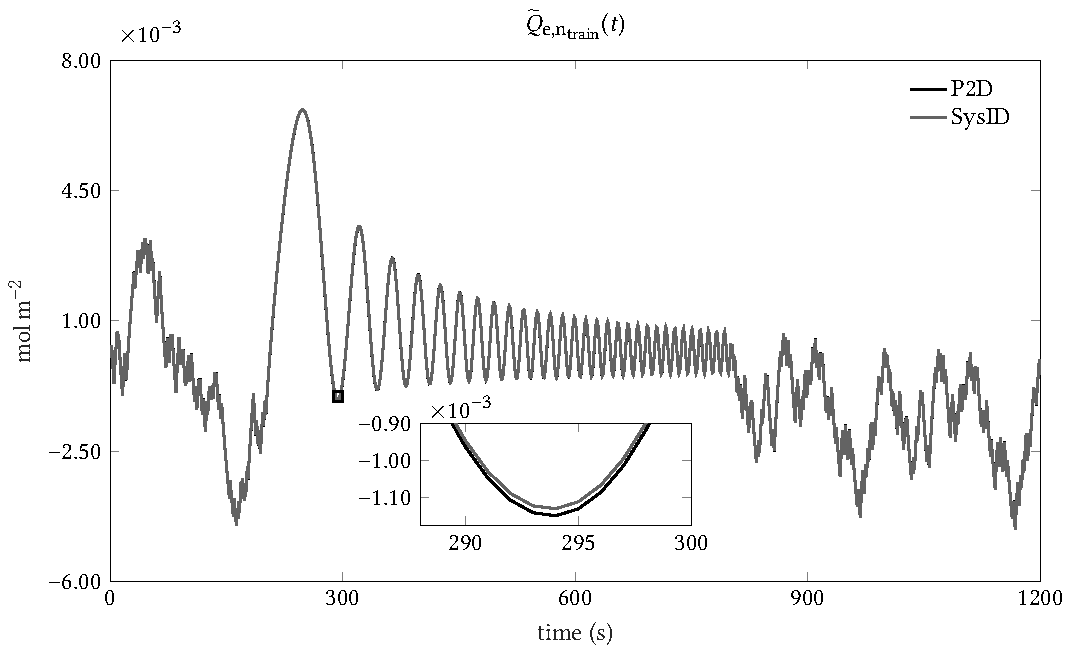
\includegraphics{chapters/sys_id/figures/p2d_sysid_train_qen.pdf}
    \caption[$\widetilde{Q}_{\text{e,n}}(t)$ outputs from \glsfmtshort{p2d} and
    identified transfer function for training profile]{%
        Time-evolution of~$\widetilde{Q}_{\text{e,n}}$ computed using the
        \glsfmtshort{p2d} model  and the identified transfer function
        of \cref{eq:finaldisctfneg} (scaled by~0.001) with the synthetic
        training input profile of \cref{fig:sysidtrainingcurrent}. The output
        predicted by the identified transfer function closely matches the `true'
        output obtained by a high-fidelity \glsfmtshort{p2d} simulation with an
        \glsfmtshort{rms} error of \SI{5.70e-6}{\mole\per\meter\squared} and a
        \glsfmtshort{mae} of~\SI{19.19e-6}{\mole\per\meter\squared}. Note that the
        transfer function in \cref{eq:finaldisctfneg} was originally obtained by
        scaling the output by~1000. The transfer function output is
        multiplied by the reciprocal of the same scaling factor to obtain the
        predicted response shown here, thereby once again justifying the
        linearity assumption for this subsystem.
    }%
    \label{fig:tfpredQentrain}
\end{figure}

\Cref{fig:tfpredQentrain} shows a comparison of the $\widetilde{Q}_{\text{e,n}}$
output for
\begin{enumerate*}[label=\emph{\alph*})]
    \item the \gls{p2d} model, and
    \item the identified transfer function of \cref{eq:finaldisctfneg}
\end{enumerate*}
using  the  training  current  profile  of \cref{fig:sysidtrainingcurrent}.  The
transfer function of \cref{eq:finaldisctfneg} was obtained by scaling the output
of the  training profile to  be of order~$\mathcal{O}(1)$  by a factor  of~1000.
Therefore,  for final  implementation and  comparison purposes,  the raw  output
produced  by applying  the transfer  function  needs to  be scaled  back by  its
reciprocal. If  the system  is linear,  then this scaling  factor shall  have no
impact  on  the  frequency-dependent  dynamics  of  the  subsystem.  The  output
predicted  by the  identified transfer  function is  virtually indistinguishable
from  the `true'  output computed  by post-processing  the \gls{p2d}  model with
an  \glsfmtshort{rms}  error   of  \SI{5.70e-6}{\mole\per\meter\squared}  and  a
\glsfmtshort{mae} of~\SI{19.19e-6}{\mole\per\meter\squared}.  This high accuracy
of the transfer  function prediction justifies the linearity  assumption for the
subsystem.  \Cref{fig:tfpredQepval}  presents  the  same  comparison  using  the
validation input profile for the subsystem in the positive electrode region. The
accuracy of  the identified transfer function  for this independent data  set is
clearly illustrated.

\begin{figure}[!htbp]
    \centering
    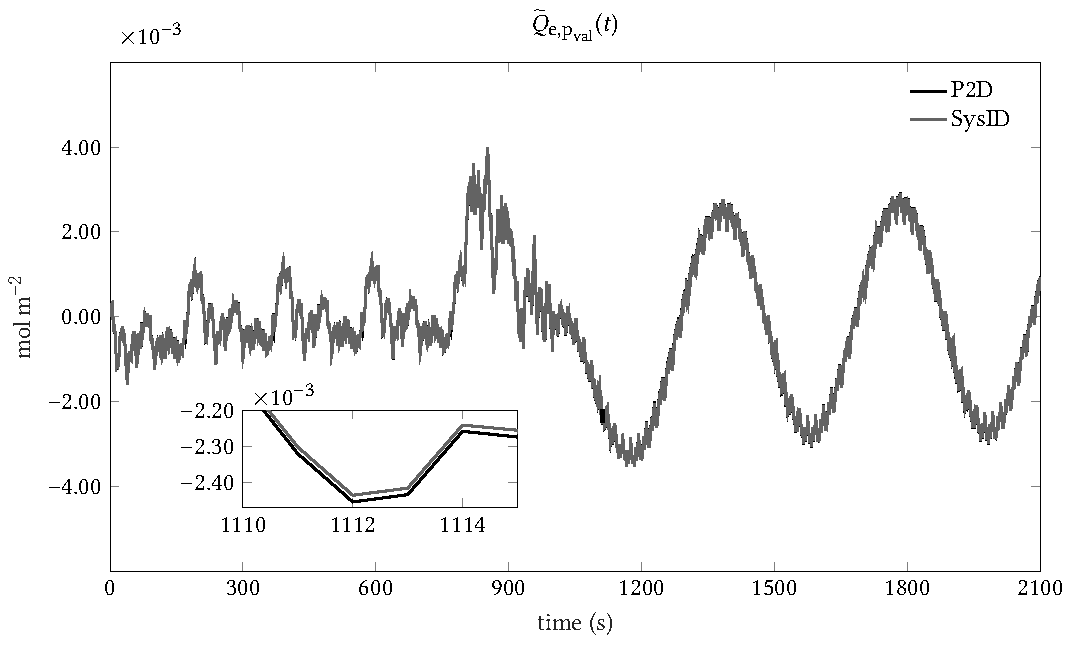
\includegraphics{chapters/sys_id/figures/p2d_sysid_val_qep.pdf}
    \caption[$\widetilde{Q}_{\text{e,p}}(t)$ outputs from \glsfmtshort{p2d} and
    identified transfer function for training profile]{%
        Time-evolution of~$\widetilde{Q}_{\text{e,p}}$ computed using the
        \glsfmtshort{p2d} model  and the identified transfer function
        of \cref{eq:finaldisctfpos} (scaled by~0.001) with the synthetic
        validation input profile of \cref{fig:sysidvalidationcurrent}. The output
        predicted by the identified transfer function closely matches the `true'
        output obtained by a high-fidelity \glsfmtshort{p2d} simulation with an
        \glsfmtshort{rms} error of \SI{12.07e-6}{\mole\per\meter\squared} and a
        \glsfmtshort{mae} of~\SI{31.59e-6}{\mole\per\meter\squared}. Note that the
        transfer function in \cref{eq:finaldisctfpos} was originally obtained by
        scaling the output by~1000. The transfer function output is
        multiplied by the reciprocal of the same scaling factor to obtain the
        predicted response shown here, thereby once again confirming the
        linearity of this subsystem.
    }%
    \label{fig:tfpredQepval}
\end{figure}

The  poles of \cref{eq:finaldisctfneg}  lie  very close  to their  corresponding
counterparts of \cref{eq:finaldisctfpos}  in the  stable region of  the Z-domain
\ie~within   the  unit  circle.   This  confirms  the  hypothesis   that  the
time-evolution subsystems  in these  two regions  exhibit similar  dynamics. The
slight differences in  the pole locations could be attributed  to the variations
in  the  physical  parameters  pertaining  to the  two  electrode  regions.  The
numerator coefficients  of \cref{eq:finaldisctfneg} and \cref{eq:finaldisctfpos}
are  also  close  to  each  other  except  that  their  signs  are  opposite  to
each   other.  This   is  to   be   expected,  since   as  seen   in  the   step
response   plots   of \cref{fig:linearity},   $\widetilde{Q}_{\text{e,n}}$   and
$\widetilde{Q}_{\text{e,p}}$ evolve in time in opposite directions. This is also
explained by  the fact  that, for  a given  applied current,  a decrease  in the
number of ions in the negative electrode has to be accompanied by an increase in
the positive electrode and vice-versa (the values of the changes are not exactly
equal owing to the presence of the separator). The identified transfer functions
are thus consistent  and deemed to be suitable for  representing the electrolyte
time-evolution in these regions.

\subsection{Numerical implementation of identified transfer functions}\label{subsec:sysidnumericalimpl}

The concept  of deploying a Z-domain  transfer function may seem  incongruous to
the  one of  the  major  goals of  this  thesis \viz~time-domain  implementation
of  \glspl{rom} in  an  embedded  environment such  as  a  \gls{bms}. While  the
majority  of the  models is  derived  and implemented  entirely in  time-domain,
only  the two  time-evolution subsystems  of  the electrolyte  seems to  deviate
from  this  trajectory.  However,  an   explanation  for  this  is  provided  in
\cref{subsec:suitablesysid}.   In  particular,   it   was   mentioned  that   an
approximation-free  conversion   to  time-domain  from  Z-domain   exists,  that
mitigates this perceived drawback for  these two sub-systems. This conversion is
amenable for discrete-time implementation without any other modifications.

Starting from the generic structure of the identified transfer functions (see \cref{eq:outputwithsysonly}),

\begin{DispWithArrows}[fleqn,mathindent=0cm,jot=2ex,%
    ,xoffset=-4mm
    ]
    G(z) &= \frac{b_1z^{-1} + \dots + b_{n_b}z^{-{n_b}}}{1 + a_1z^{-1} + \dots + a_{n_a}z^{-{n_a}}} \Arrow{Replace with analogous \\ transfer operator $q=z$ \\ in time domain} \notag\\
    G(q) &= \frac{b_1q^{-1} + \dots + b_{n_b}q^{-{n_b}}}{1 + a_1q^{-1} + \dots + a_{n_a}q^{-{n_a}}} \Arrow{Apply the definition\\ of~$G(q)$ on the \glsfmtshort{lhs}}\notag \\
    \frac{y[k]}{u[k]} &= \frac{b_1q^{-1} + \dots + b_{n_b}q^{-{n_b}}}{1 + a_1q^{-1} + \dots + a_{n_a}q^{-{n_a}}} \Arrow{Cross-multiply}\notag \\
    \left(1 + a_1q^{-1} + \dots + a_{n_a}q^{-{n_a}}\right)y[k] &= \left(b_1q^{-1} + \dots + b_{n_b}q^{-{n_b}}\right)u[k] \Arrow{Expand on both sides} \notag \\
    y[k] + a_1q^{-1}y[k] + \dots + a_{n_a}q^{-{n_a}}y[k] &= b_1q^{-1}u[k] + \dots + b_{n_b}q^{-{n_b}}u[k] \Arrow{Apply the definition\\ $q^{-p}x[k] = x[k-p]$}\notag \\
    y[k] + a_1y[k-1] + \dots + a_{n_a}y[k-n_a] &= b_1u[k-1] + \dots + b_{n_b}u[k-n_b] \Arrow{Rearrange to obtain\\ the final expression}\notag \\
    y[k] &= -a_1y[k-1] - \dots - a_{n_a}y[k-n_a] \notag \\[-2ex]
         &\qquad   + b_1u[k-1] + \dots + b_{n_b}u[k-n_b] %\label{eq:lccde}
\end{DispWithArrows}

We  thus obtain  a  simple  algebraic expression  (a  difference equation)  that
computes the output  at the given time-step given past  inputs and outputs. This
is a highly memory-efficient implementation  since, at any given time-step, only
the previous~$n_a$ (four) output samples  and $n_b$ (four) input samples need to
be  `remembered'  (stored).  This  concludes all  the  aspects  (derivation  and
implementation) of  this author's new  model for the  electrolyte time-evolution
subsystem.  The  performance  of  this  model  for  computation  of  electrolyte
concentration needs to be evaluated, which is performed next.



\section{Performance Analysis of New Model: Ionic Concentration}\label{sec:perfanalysisnewmodel}
% -*- root: ../main.tex -*-
%!TEX root = ../main.tex
% this file is called up by main.tex
% content in this file will be fed into the main document
% vim:textwidth=80 fo=cqt

To demonstrate that a suitable advancement of the field has indeed been achieved
through  this system  identification exercise,  a comparison  with the  existing
state of the art in reduced  order electrolyte modelling is warranted. Secondly,
to  comprehend its  extent of  validity  and performance  boundaries, the  newly
developed \gls{rom} must also be  pitted against the full-order \gls{p2d} model.
This section  aims to  provide such  a comparative discussion  for two  types of
inputs ---
\begin{enumerate*}[label=\itshape\alph*\upshape)]
    \item constant current inputs
    \item dynamic load profiles
\end{enumerate*}

\subsection{Constant current inputs}\label{subsec:tfquadceconstcurrinput}

\Cref{fig:tfquadp2dspatialionicconc1C} shows  the spatial distribution  of ionic
concentration  in  the electrolyte  along  cell  thickness  for a  1C  discharge
beginning at \SI{100}{\percent} \gls{soc}. The spatial concentration computed by
each of the three approaches ---
\begin{enumerate*}[label=\roman*)]
    \item the \gls{p2d} model,
    \item the quadratic approximation model and
    \item the newly developed system identification model(s).
\end{enumerate*}

\begin{figure}[!htbp]
    \centering
    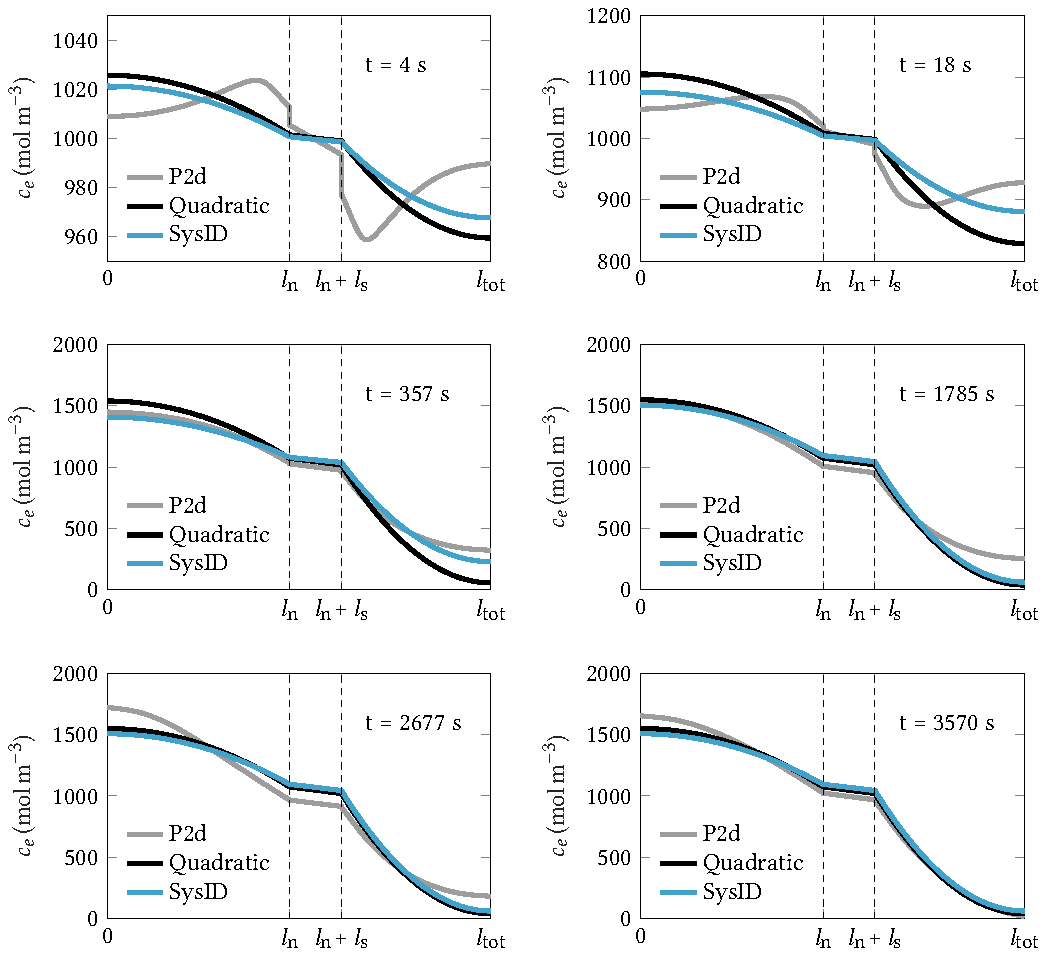
\includegraphics[width=\textwidth]{tf_quadratic_ce_approx_spatial.pdf}
    \caption[Spatial distribution of ionic concentration in
    electrolyte for a 1C discharge computed by the \glsfmtshort{p2d}, quadratic
    approximation \& system identification models]{%
        Spatial distribution of ionic concentration  in electrolyte along cell
        thickness at various  snapshots of  time computed  by each of  the three
        models for  a 1C discharge.  The concentration  profile  computed by
        the  \gls{p2d} model is used as the benchmark reference. The  system
        identification model performs noticeably better than the quadratic
        approximation model during  the initial  transient  while delivering a
        similar performance as a \gls{qss} is reached.
}%
\label{fig:tfquadp2dspatialionicconc1C}
\end{figure}

During  the  initial  phase  of   discharge,  the  \gls{p2d}  model  exhibits  a
characteristic inflection point near the  separator interfaces that diffuses out
over time  until a  \gls{qss}. This  is due to  the fact  the reaction  front is
initially established  close to the  separator, and as surface  concentration of
lithium  in particles  near separator  is  depleted, the  reaction starts  moves
further  into the  electrode thickness.  Neither  of the  two \glspl{rom}  under
consideration here  could successfully  capture this  characteristic inflection.
This is  explained by  the fact  that both  of them  use the  standard quadratic
approximation profile for the \emph{spatial}  profile, which means that only one
apex  point is  possible  per  electrode, which  is  pinned  to their  separator
interfaces by design.

During the transient portion of discharge (approximately up to \SI{357}{\second}
as   shown   in \cref{fig:tfquadp2dspatialionicconc1C}),   the  locus   of   the
concentration  profile computed  by  the newly  developed system  identification
model(s) clearly lies  much closer to the \gls{p2d} model  than that computed by
the  quadratic  approximation model.  After  the  initial transition  phase,  it
appears  that  the  concentration  profile predicted  by  both  the  \glspl{rom}
converge to the \gls{p2d} model's concentration profile.


To obtain  a quantifiable  perspective on  the accuracy  of the  newly developed
model, it  is desirable  to plot  the temporal  evolution of  the concentration,
particularly  at  the  two  current   collector  interfaces.  The  behaviour  of
the  baseline  quadratic approximation  model  in  this regard  was  established
in \cref{subsubsec:simresultsbaselinequad}.   Therefore  it   is  important   to
ascertain whether a noteworthy improvement  was achieved using the model arrived
at using the system identification procedure.

\begin{figure}[!htbp]
    \centering
    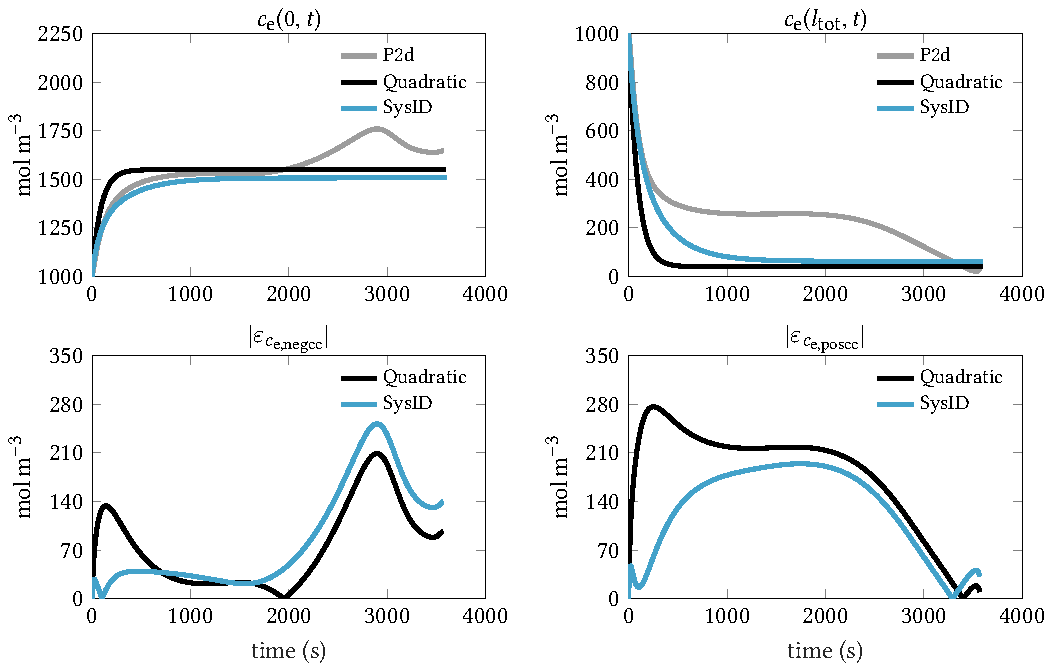
\includegraphics[width=\textwidth]{tf_quad_ce_at_cc_1Cdischg}
    \caption[%
    Time evolution  of ionic  concentrations at  current collectors  computed by
    \glsfmtshort{p2d}, quadratic  approximation \& system  identification models
    for 1C discharge
    ]%
    {%
    Evolution  of ionic  concentration over  time at  the two  current collector
    interfaces for a 1C discharge for
    \begin{enumerate*}[label=\roman*)]
        \item the \glsfmtshort{p2d} model,
        \item the quadratic approximation model and
        \item the newly developed system identification model(s)
    \end{enumerate*}
    (top row). For the quadratic approximation and system identification models,
    the time evolution of their absolute error relative to the \glsfmtshort{p2d}
    benchmark  is also  shown  (bottom  row). At  both  current collectors,  the
    transient performance of the system  identification model is superior to the
    quadratic  approximation model.  At \gls{qss},  the quadratic  approximation
    model is slightly more accurate than the system identification model.
}%
\label{fig:temporalcetfquadratic}
\end{figure}

\Cref{fig:temporalcetfquadratic}   shows  the   time-evolution   of  the   ionic
concentrations at the current collector  interfaces of the negative and positive
electrodes for a 1C discharge. The  concentration profiles computed
by the three approaches ---
\begin{enumerate*}[label=\roman*)]
    \item \glsfmtshort{p2d} model,
    \item quadratic approximation model and the
    \item newly developed system identification model(s)
\end{enumerate*}
are overlaid in the top row of  plots, wherein the left hand side corresponds to
the  current collector  interface  at  the negative  electrode  while the  right
hand  side  corresponds  to  that  at  the  positive  electrode.  The  plots  in
the bottom  row of \cref{fig:temporalcetfquadratic}  show the  time-evolution of
the  absolute  value  of  their  errors. The  concentration  error  of  each  of
the  two  \glspl{rom}  is  defined  with  respect  to  the  benchmark  \gls{p2d}
model  \ie~$\varepsilon_{c_{\text{e,}j}(t)}   =  c_{\text{e,}j_\text{ROM}}  -
c_{\text{e,}j_\text{p2d}}(t)$. The  absolute value  of the  error is  plotted so
that  the magnitude  of the  error can  be visualised  better, aiding  immediate
comparisons based on the plots.

For both  current collectors,  the newly  developed system  identification model
outperforms the  quadratic approximation  model during  the transient  phase. At
the  negative electrode/current  collector interface,  the error  of the  system
identification model remains strictly below  that of the quadratic approximation
model until \approx \SI{650}{\second} and remains comparable to it until \approx
\SI{1600}{\second}. Beyond  this time, the  quadratic approximation model  has a
slightly better accuracy, although the system identification model still remains
at a comparable distance from  it. After \approx \SI{2000}{\second}, both models
yield  the same  response shape.  For the  positive electrode/current  collector
interface, the  error of the system  identification model remains below  that of
the quadratic approximation model until \approx \SI{3300}{\second}.

\begin{figure}[!htbp]
    \centering
    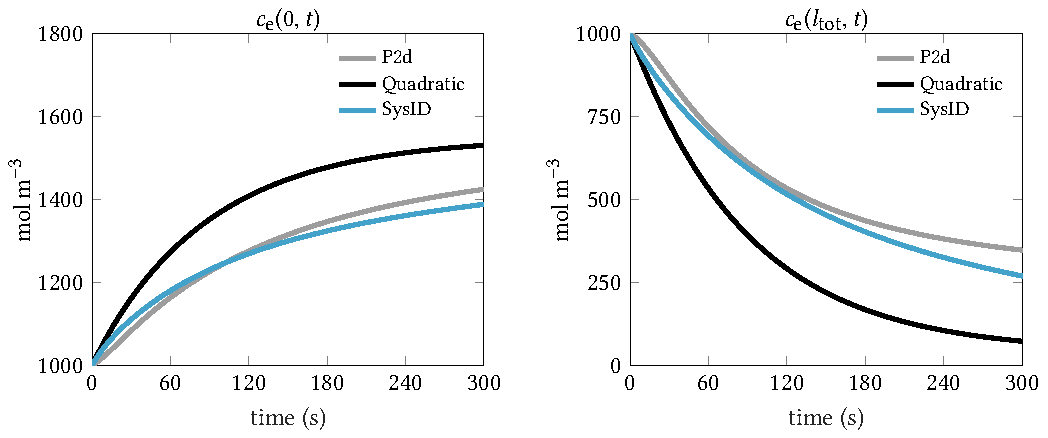
\includegraphics[width=\textwidth]{zoomed_tf_quad_ce_at_cc_1Cdischg.pdf}
    \caption[%
    Transient phase of ionic  concentration evolution at  the two current collectors  computed by
    \glsfmtshort{p2d}, quadratic  \& system  identification models
    for 1C discharge
    ]%
    {%
    Transient phase of the temporal evolution  of ionic  concentration at  the two  current collector
    interfaces for a 1C discharge as computed by ---
    \begin{enumerate*}[label=\roman*)]
        \item the \glsfmtshort{p2d} model,
        \item the quadratic approximation model, and
        \item the newly developed system identification model(s).
    \end{enumerate*}
    The significantly improved accuracy of the system identification model(s)
    relative to the state of the art quadratic approximation model is clearly demonstrated.
}%
\label{fig:zoomedcetfquadtemporal}
\end{figure}

\Cref{fig:zoomedcetfquadtemporal} shows  a zoomed version of  the time-evolution
of the  ionic concentration  at the  two current  collectors, wherein  the first
\SI{300}{\second}  after  application  of  the  load  current  is  plotted.  The
significant  improvement in  accuracy  achieved by  the  newly developed  system
identification model(s) is clearly demonstrated. At both the current collectors,
the concentration computed  by the system identification  model(s) closely track
that of the benchmark \gls{p2d} model.

The  loss  of fidelity  exhibited  past  the  initial transient  phase  warrants
an  explanation. It  should  be  recalled that  the  natural  decoupling of  the
temporal and  spatial systems were taken  advantage of in developing  the system
identification technique. This  means that, for the spatial  profile, the system
identification  model reverts  to the  same  quadratic profile  as the  baseline
quadratic approximation  model. This  explains why the  two models  have similar
shape past the initial transient. During  the transient phase when the \gls{qss}
behaviour is yet to be established, it is reasonable to assume that the temporal
dynamics  are of  paramount importance  in governing  the concentration  profile
evolution.  After a  \gls{qss}  has  been established  with  the reaction  front
diffusing out  and a steady  stream of ion-electron  separation/recombination in
place,  it is  hypothesised  that the  temporal dynamics  have  settled and  the
spatial configuration assumes importance.

With a  sustained application  of constant current  past the  initial transient,
strong spatial gradients  in the ionic concentration are  established within the
cell \ie~the  concentrations are far from the initial  equilibrium value. This
precisely  exposes the  realm  where the  system  identification model  exhibits
its  natural  weakness.  By  following  the  theory  of  system  identification,
which  necessitates   bias  removal,   the  training  and   validation  profiles
of \cref{fig:sysidtrainingcurrent}   and \cref{fig:sysidvalidationcurrent}   had
nearly  zero mean.  This means  that the  currents were  as equally  positive as
negative leading to a small-signal  perturbation around the equilibrium value of
the electrolyte  concentration. While this  profile is ideally suited  to excite
the system's  dynamics, it  fails to  capture the large  signal behaviour.  As a
topic  of future  research,  perhaps a  spatially-coupled system  identification
could be attempted to handle this issue.

The  main  implication of  these  results  is  that  the identified  models  are
primarily suitable for  transient \ie~dynamic load profiles,  which is typical
of a real-life scenario in an electric/hybrid electric vehicular operation. Such
a  model is  less  suitable  for sustained  constant  current application.  This
implies that  a \gls{bms} in a  vehicle undergoing a \gls{cccv}  charging cannot
rely on  these identified electrolyte  models. However, this exclusion  does not
seriously hamper the model's wider applicability since a simple coulomb-counting
approach with  a high-precision \gls{adc} is  much more accurate than  any other
physics based model in this particular scenario.

Although constant  current discharge is  not a practical use-case  for vehicular
batteries, performing this benchmark evaluation  has helped in understanding the
limits of the newly  developed model. This study has also  helped in providing a
glimpse of its  potential strength \viz~significantly  improved accuracy under
dynamic load conditions, which is presented next.

\subsection{Dynamic current inputs}

To characterise  the performance  of the  newly developed  system identification
electrolyte   concentration  model(s)   under  dynamic   load  conditions,   the
\gls{udds}  drivecycle  was  used.  The  details  of  this  drivecycle  such  as
its  speed  versus  time  data  and its  highly  dynamic  nature  was  discussed
in \cref{subsubsec:dynamicspmp2dsim}. The peak of  the applied load current used
corresponds to a discharge current of \SI{180}{\ampere} \ie~3C. A plot of this
current  profile was  shown in  the top  row of \cref{fig:uddssimp2dspmresults}.
This  load  profile  was  applied   to  the  three  models  under  consideration
---
\begin{enumerate*}[label=\itshape\alph*\upshape)] \item \glsfmtshort{p2d}
model,  \item   quadratic  approximation   model,  and  \item   newly  developed
system identification  model(s) \end{enumerate*} ---
and the spatio-temporal evolution of ionic concentration in electrolyte computed
by each of them was studied.

Since  the  load   current  is  highly  dynamic   and  continuously  alternating
between  charging   and  discharging   at  various  magnitudes   throughout  the
profile   duration,   it   is   difficult  to   discern   a   specific   pattern
or   trend  within   the  spatial   thickness   of  the   cell.  Hence,   unlike
the   case   of  prolonged   unidirectional   current   application  wherein   a
clear   reaction  front   that  diffuses   gradually  out   can  be   visualised
(see \cref{fig:tfquadp2dspatialionicconc1C}), little  information can  be gained
from  visualisation   of  spatial   concentration  profiles.  Since   the  ionic
concentrations at  the two  current collectors have  a direct  (and two-pronged)
influence on the  electrolyte overpotential (see \cref{eq:electrolytepdwithce}),
it is particularly important to characterise  the accuracy at these two critical
spatial locations.

Since a  direct correspondence between  the time-dependent dynamics of  the load
profile and that of the electrolyte concentration can be intuitively visualised,
its values  at the two current  collector interfaces are examined.  The plots in
the top row of \cref{fig:uddsTfQuadCeatCC} shows the time evolution of the ionic
concentration at the two current  collector locations for the \gls{udds} current
profile computed by  each of the three models under  consideration. The plots to
the left  pertain to the negative  current collector location while  that to the
right correspond to  the positive current collector location. The  bottom row of
plots show the absolute value of concentration error of the quadratic and system
identification models relative to the  \gls{p2d} reference benchmark. As seen in
in \cref{fig:uddsTfQuadCeatCC}, the absolute error of the newly developed system
identification models remain below that  of the baseline quadratic approximation
model throughout the drivecycle.

\begin{figure}[!htbp]
    \centering
    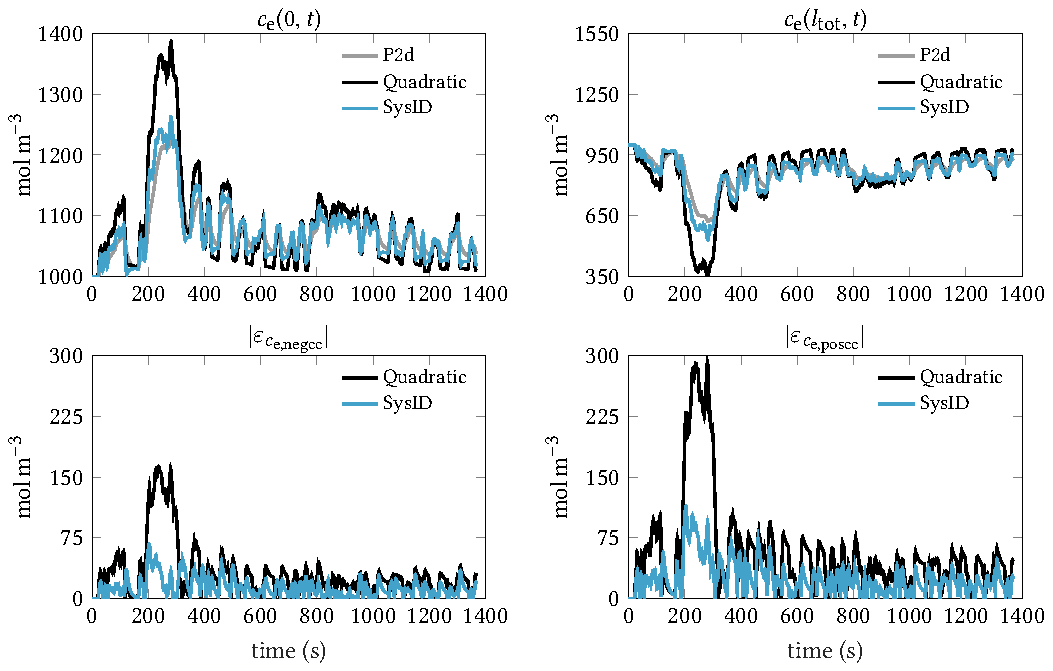
\includegraphics[width=\textwidth]{tf_quad_ce_at_cc_udds}
    \caption[%
    Time   evolution  of   ionic  concentrations   at  current   collectors  for
    \glsfmtshort{p2d}, quadratic  approximation \& system  identification models
    with a \glsfmtshort{udds} input profile
    ]%
    {%
        Evolution of ionic concentration over  time at the two current collector
        interfaces with  a \gls{udds}  input profile (see  topmost plot
        of \cref{fig:uddssimp2dspmresults}) as computed by
        \begin{enumerate*}[label=\roman*)]
            \item the \glsfmtshort{p2d} model,
            \item the quadratic approximation model and
            \item the newly developed system identification model(s)
        \end{enumerate*}
        (top   row).  The   plots  on   the   left  pertain   to  the   negative
        electrode/current  collector   interface,  while   that  on   the  right
        corresponds to  the positive electrode/current collector  interface. For
        the  quadratic approximation  and  system  identification models,  their
        absolute error relative to the \glsfmtshort{p2d} benchmark is also shown
        (bottom  row).  The system  identification  model  is considerably  more
        accurate  than the  quadratic approximation  model for  the entire  time
        horizon of the drivecycle.
    }%
    \label{fig:uddsTfQuadCeatCC}
\end{figure}

Based   on   the   conclusions   from   the   constant   current   input   study
of \cref{subsec:tfquadceconstcurrinput},  it   is  to   be  expected   that  the
system  identification  model(s)  exhibit  a  superior  performance  during  the
transient  phase   of  the   simulation.  As  seen   in  the   initial  duration
of \cref{fig:uddsTfQuadCeatCC}, the absolute error  of the system identification
model is indeed  lower than that of the baseline  quadratic approximation model.
Particular, when a sudden current spike is applied at \approx \SI{200}{\second},
the  quadratic approximation  model is  unable to  cope and  its absolute  error
deviates  far  away   from  its  mean  value.  The  absolute   error  of  system
identification model  remains well controlled  and even with  this instantaneous
load demand, its standard deviation is remarkably close to its median value as
shown in \cref{tbl:errormetricsquadtfce}.

% -*- root: ../../main.tex -*-
%!TEX root = ../../main.tex
% this file is called up by main.tex
% content in this file will be fed into the main document
% vim:textwidth=180 fo=cqt conceallevel=0

\begin{table}[!htbp]
    \centering
    \caption[Error statistics for the quadratic approximation \& system identification models]{Summary of error statistics for the quadratic approximation and system identification models. The metric used is the absolute value of the concentration difference with respect to the \glsfmtshort{p2d} model at the two current collector interfaces.}
    \label{tbl:errormetricsquadtfce}
    \begin{tabular}{@{} l S[table-format=3.2] S[table-format=3.2] S[table-format=3.2] S[table-format=3.2] @{}}
        \toprule
        \multirow{2}[2]{*}{\makecell{Error  statistic \\ (\si{\mole\per\meter\cubed})}} & \multicolumn{2}{c}{$\big\lvert \varepsilon_{c_\text{e}} \big \rvert$ at Neg/CC} &
        \multicolumn{2}{c}{$\big\lvert \varepsilon_{c_\text{e}} \big \rvert$ at Pos/CC} \\
        \cmidrule(lr){2-3} \cmidrule(l){4-5}
        {} & {Quadratic} & {SysID} & {Quadratic} & {SysID} \\
        \midrule
        Max                & 307.27 & 190.04 & 292.20 & 114.44 \\
        Mean               & 66.38  & 54.98  & 55.15  & 25.02  \\
        Median             & 49.65  & 47.12  & 40.39  & 20.93  \\
        Standard Deviation & 66.80  & 37.18  & 60.50  & 20.17  \\
        \bottomrule
    \end{tabular}
\end{table}


While the  superior accuracy of the  newly developed model during  the transient
phase  was not  surprising, the  fact  that its  performance remains  consistent
throughout  the  entire  time  horizon  is  noteworthy.  Despite  being  subject
to  incessant  changes   in  load  demands,  the   system  identification  model
responds better  than the  quadratic approximation model  well past  the initial
transient.  \Cref{fig:zoomedcetfquadtemporaludds} shows  a  zoomed  view of  the
ionic concentration in the electrolyte  at the two current collector interfaces.
To prove the improved performance of the developed model well into the operation
of the cell, a \SI{50}{\second} window beginning at \approx \SI{60}{\percent} of
the overall  profile duration is examined  in detail. Although it  exhibits some
oscillations,  the system  identification model(s)  reasonably track  the `true'
concentrations computed by the \gls{p2d}  model. However, the baseline quadratic
approximation  model seems  to suffer  from  a large  bias with  respect to  the
\gls{p2d} model.  It should also  be noted that nearly  every `kink' in  the two
\glspl{rom}  is identical.  This could  be attributed  to the  fact the  spatial
profile  used  in  both of  them  is  identical.  Hence,  it must  be  concluded
that  the difference  in their  amplitude arises  from the  improved calculation
of coefficients~$a_k(t)$ in \cref{eq:cenqquadstart} and \cref{eq:cepqquadstart}
through  the  usage  of  more  accurate  $Q_{\text{e,n}}$  and  $Q_{\text{e,p}}$
in  the  \gls{lhs} of \cref{eq:Qenbyintegration}  and \cref{eq:Qepbyintegration}
respectively.  Detailed   error  metrics  of   the  two  \glspl{rom}   is  shown
in \cref{tbl:errormetricsquadtfce}.

\begin{figure}[!htbp]
    \centering
    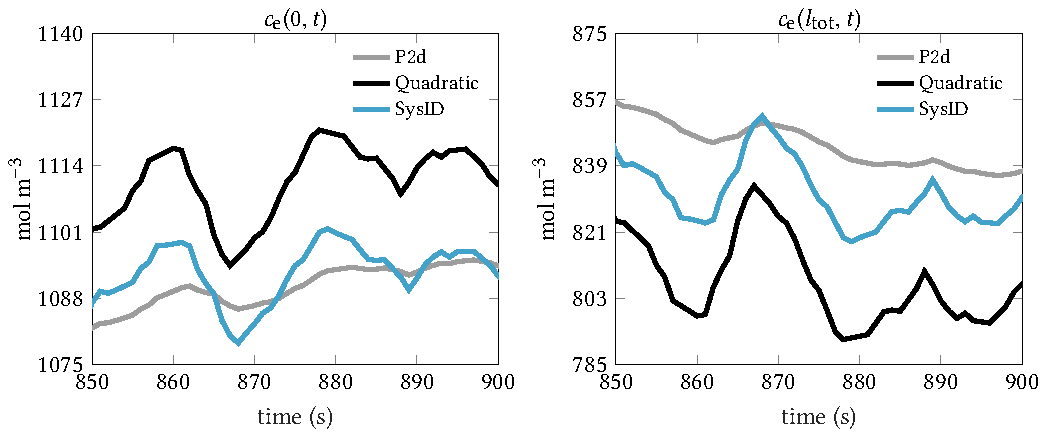
\includegraphics[width=\textwidth]{zoomed_tf_quad_ce_at_cc_udds}
    \caption[%
    Zoomed view of ionic  concentration at  both current collectors  computed by
    the \glsfmtshort{p2d}, quadratic  \& system  identification models
    for the \glsfmtshort{udds} profile
    ]%
    {%
        A zoomed  view of  the ionic  concentration (showing  a \SI{50}{\second}
        window  beginning at  \approx \SI{60}{\percent}  of the  overall profile
        duration) in the electrolyte at the two current collector interfaces for
        the \gls{udds} profile of \cref{fig:uddssimp2dspmresults} as computed by
        ---
        \begin{enumerate*}[label=\roman*)]
            \item the \glsfmtshort{p2d} model,
            \item the quadratic approximation model, and
            \item the newly developed system identification model(s).
        \end{enumerate*}
        At both current collector interfaces, the system identification model(s)
        exhibits  a reasonable  tracking of  the concentration  profile computed
        by  the  benchmark \gls{p2d}.  The  profile  computed by  the  quadratic
        approximation  model  seems  to  suffer from  offsets/bias  issues  that
        adversely affects its accuracy.
}%
\label{fig:zoomedcetfquadtemporaludds}
\end{figure}

Based  on  the  evidence presented  thus  far,  it  can  be concluded  that  the
time-evolution subsystem model(s) developed here using the system identification
technique  indeed  represent  an  advancement  of the  field  of  reduced  order
electrolyte  modelling. With  this  aspect  thus tackled,  it  is imperative  to
explore the potential benefits of  incorporating the discrete-time model(s) thus
obtained into the conventional \gls{spm} and is discussed next.


\section{Composite SPM Model with Electrolyte Dynamics}
% -*- root: ../../main.tex -*-
%!TEX root = ../../main.tex
% this file is called up by main.tex
% content in this file will be fed into the main document
% vim:textwidth=80 fo=cqt

At this  stage, it must  be recalled that the  purpose of developing  the system
identification electrolyte  model was  to mitigate the  poor performance  of the
basic  \gls{spm} at  C-rates above~0.5C (see \cref{subsec:simresultsbasicspm}).
This sub-optimal performance was attributed  to the lack of electrolyte dynamics
in  the  basic  \gls{spm}.  The   performance  of  the  newly  developed  system
identification model has been proved to be  superior to the current state of the
art. The next step  is to embed this electrolyte model  into the basic \gls{spm}
so as to  obtain a composite \gls{spm}. The performance  of this composite model
is evaluated to ascertain its suitability towards online implementation.

\subsection{Computation of electrolyte overpotential}\label{subsec:electrolyteopcalc}

The missing component in the terminal voltage computation of the basic \gls{spm}
is  the  contribution from  the  electrolyte  overpotential  term. This  is  the
potential difference in  the entire electrolyte \ie~the electrolyte potential
at the positive current collector interface with respect to that at the negative
current collector interface.


As discussed in \cref{sec:electrolyteinclusion}, using  the equation proposed by
Prada~\etal~\cite{Prada2012}, the  overpotential in the electrolyte  is computed
as
\begin{align}
    \quad \phi_\epos - \phi_\eneg &= (1-t_{+}^0) \frac{2RT}{F}\ln \frac{c_\text{e,\tiny pos/cc}}{c_\text{e,\tiny neg/cc}}\nonumber\\
    {} &\quad -\frac{I}{2 A}\left(\frac{l_\text{neg}}{\kappa_\text{eff,neg}} + 2 \frac{l_\text{sep}}{\kappa_\text{eff,sep}} + \frac{l_\text{pos}}{\kappa_\text{eff,pos}}\right) \tag{\cref{eq:electrolytepdwithce} revisited}
\end{align}

\Cref{eq:electrolytepdwithce} consists of two distinct terms ---
\begin{enumerate*}[label=\roman*)]
    \item a diffusion overpotential due to concentration gradient in the electrolyte, and
    \item an ohmic resistance term that is dependent upon
        \begin{enumerate*}[label=\itshape\alph*\upshape)]
            \item the instantaneous value of applied current,
            \item the thicknesses of the three cell regions, and
            \item the effective ionic conductivity in each of the three regions. %which in-turn depends on ionic concentration,.
        \end{enumerate*}
\end{enumerate*}

The ohmic  loss term  of \cref{eq:electrolytepdwithce} needs  to be  examined in
closer detail.  The dependence of  this term  on instantaneous load  current and
cell thicknesses  can be accounted  in a straightforward manner.  However, there
are ambiguities  in computing the  effective ionic  conductivity in each  of the
three cell regions. The effective value of ionic conductivity in the electrolyte
depends on its intrinsic conductivity, the Bruggeman constants and porosities of
each  of  the three  regions.  The  intrinsic electrolyte  conductivity  in-turn
depends on the electrolyte concentration.

Ambiguities   arise   in  interpreting   the   value   of  ionic   concentration
to   be    used   for   computation   of    electrolyte   concentration.   Since
\cref{eq:electrolytepdwithce}  deals  with  overall potential  drop  across  the
entire  length of  the cell,  the concentration  used for  computing electrolyte
conductivity could,  for example be  that at the respective  current collectors.
This concept however  introduces inconsistencies with the  separator term. Using
the  separator concentration  from one  of the  electrode interfaces  introduces
unequal  weighting  in this  computation.  If  the  ionic concentration  at  the
midpoint of the separator is used, this scheme becomes inconsistent with that at
the  two current  collectors. Another  possibility for  computing the  effective
conductivity in a  cell region is to  use the mean of the  concentration in that
region. However, since the mean is nothing but a simple statistical first moment
is  equally influenced  by the  entire  concentration profile  within each  cell
region. This is questionable given that the electrolyte overpotential across the
entire cell thickness  is most likely governed by the  conductivities at the two
current  collector interfaces.  Some form  of weighted  mean could  be conjured,
wherein the  current collector locations  are given  the highest weight  and the
separator locations the  least weight. However, finding the  weights becomes yet
another  exercise and  from the  engineering perspective  of computing  these in
real-time, seems to be in the realm of diminishing returns.

In  published  literature,  only  a  cursory  treatment  has  been  accorded  to
the  aforementioned  ambiguities.  In  Prada~\etal~\cite{Prada2012},  the  usage
of  initial concentrations  is  used  to only  introduce  the  concept of  ohmic
resistance  in that  article.  However,  the author  of  this  thesis wishes  to
extend  this  concept further.  In  the  simulations  conducted by  this  thesis
author, it  became clear  that the  dependence on  applied current  was required
in  order to  obtain  reasonable accuracies.  Computing  mean of  concentrations
in  cell  regions for  calculation  of  ionic  conductivities  led to  a  biased
computation of overpotentials.  Therefore, this author decided to  use the value
of  initial concentration  for the  computation of  ionic conductivities  in the
current-dependent  contribution  to  electrolyte  overpotential  throughout  the
entire time horizon considered.

Hence, as per the adopted scheme \cref{eq:electrolytepdwithce} gets modified as
\begin{align}
    \quad \phi_\epos(t) - \phi_\eneg(t) & = (1-t_{+}^0) \frac{2RT}{F}\ln \frac{c_\text{e,\tiny pos/cc}(t)}{c_\text{e,\tiny neg/cc}(t)}\nonumber \\
    {}                             &\quad -\frac{I}{2 A}\left(\frac{l_\text{neg}}{\kappa_\text{eff,neg}\left(c_\text{e}\left(0\right)\right)} + 2
    \frac{l_\text{sep}}{\kappa_\text{eff,sep}\left(c_\text{e}\left(0\right)\right)} +
\frac{l_\text{pos}}{\kappa_\text{eff,pos}\left(c_\text{e}\left(0\right)\right)}\right)\label{eq:electrolytepdwithcenew}
\end{align}
wherein  the time-dependent terms are explicitly shown in the notation.

Using \cref{eq:electrolytepdwithcenew} for electrolyte overpotential computation
has an  important implication. The  two-pronged influence of  the time-dependent
electrolyte concentration on the electrolyte overpotential \viz
\begin{enumerate*}[label=\itshape\alph*\upshape)]
    \item a direct influence in the form of concentration dependent diffusion polarisation, and
    \item an indirect influence through its use in ionic conductivity calculations
\end{enumerate*}
has  now  been  reduced  to  just   one.  This  implies  the  results  from  the
system  identification   model  are  now   required  only  in  the   first  term
of \cref{eq:electrolytepdwithcenew}.

In the light of the decision of use the (constant) initial concentration for the
ohmic term, it is natural to question the gains from the circuitous route of the
system  identification  exercise that  was  undertaken  to obtain  the  improved
electrolyte model. Therefore,  it is imperative to quantify  the relative weight
of  the  concentration  dependent  diffusion resistance  compared  to  the  bulk
solution resistance.

\begin{figure}[!htbp]
    \centering
    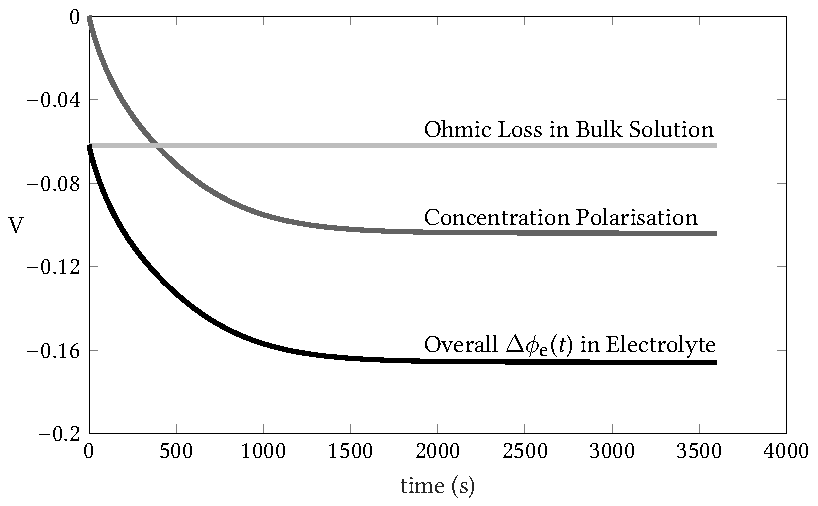
\includegraphics{contribution_to_phie_1C.pdf}
    \caption[%
    Contribution to electrolyte overpotential from the gradient-induced polarisation
    term and the bulk solution resistance term for a 1C~discharge
    ]%
    {%
        Contribution to the overpotential in the electrolyte from each of the
        two terms in \cref{eq:electrolytepdwithcenew} for a 1C~discharge. The
        bulk solution resistance is approximated as a constant value determined
        by the equilibrium initial concentration. The concentration dependent
        polarisation term governs the dynamic behaviour of the overall
        overpotential. Furthermore, this gradient-induced diffusion resistance
        has a strong contribution to the steady state, higher than the bulk
        solution resistance and cannot be neglected without introducing
        significant errors.
}%
\label{fig:contributiontophiefromtwoterms}
\end{figure}

\Cref{fig:contributiontophiefromtwoterms} shows the  contribution to the overall
potential drop~$\phi_\text{e,pos}$ and~$\phi_\text{e,neg}$ in  the electrolyte
from  each  of  the  two  terms  in \cref{eq:electrolytepdwithcenew}  for  a  1C~discharge. The bulk  solution resistance is constant owing to  the fact that the
initial  electrolyte concentration  is  used in  computing  the effective  ionic
conductivities in the three regions of  the cell. The gradient induced diffusion
polarisation term, however has a stronger contribution in both the transient and
steady  state. The  entire dynamics  of the  overall potential  drop during  the
transient  phase is  governed by  this concentration-dependent  term, while  its
steady state contribution  is in-fact higher than the  bulk solution resistance.
The  constant  ohmic resistance  term  merely  provides  a non-zero  offset  for
the  electrolyte  solution  overpotential.  In questioning  whether  the  system
identification exercise was indeed worthwhile,  if the concentrations in the two
current collectors had not been computed  at each time-step, then this diffusion
polarisation  term  would  become  zero.  This is  because,  the  numerator  and
denominator in \cref{eq:electrolytepdwithcenew} would have to be retained at the
initial concentration, leading to a unit  ratio whose natural logarithm is zero.
Therefore, it  is clear  that computing  the concentrations  at the  two current
collectors  through system  identification has  indeed helped  in improving  the
modelling accuracy.

Having established the relative  importance of computing the diffusion-dependent
polarisation   overpotential,  the   next  question   that  arises   is  whether
the   constant    approximation   for   the   bulk    solution   resistance   is
indeed   appropriate.   It  also   remains   to   be   seen  if   the   accurate
computation   of  the   ionic   concentration   through  system   identification
(see \cref{sec:perfanalysisnewmodel}) has  translated into a  similarly accurate
computation of  electrolyte overpotential. This  is answered by a  comparing the
electrolyte overpotential computed by the  system identification model with that
obtained from the \gls{p2d} model.

\begin{figure}[!htbp]
    \centering
    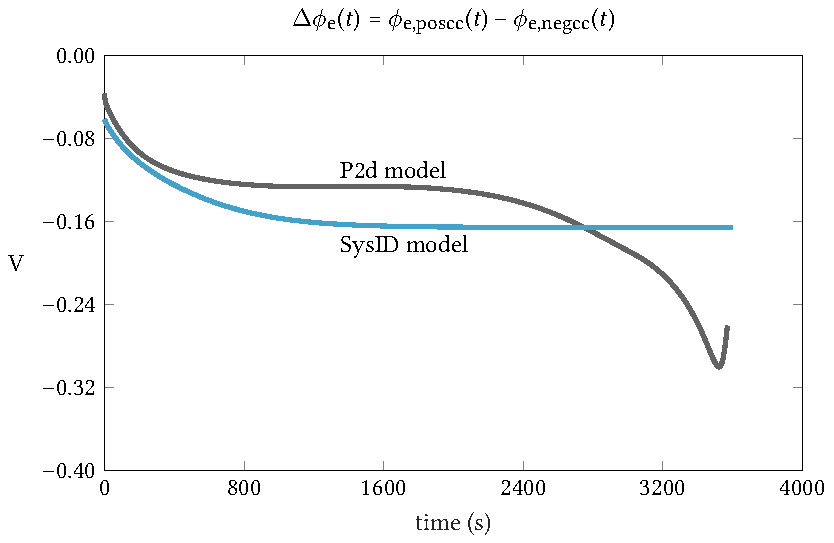
\includegraphics{phie_delta_cnst_1C.pdf}
    \caption[%
    Electrolyte  overpotential  computed  by the  \glsfmtshort{p2d}  and  system
    identification models for a 1C~discharge
    ]%
    {%
        Comparison    of    electrolyte    overpotential   computed    by    the
        \gls{p2d}     model    and     the    system     identification    model
        (using \cref{eq:electrolytepdwithcenew}) for a  1C~discharge. During the
        transient phase, the profile obtained by the system identification model
        closely matches that of the \gls{p2d} model. The mismatch in the initial
        overpotential does not arise to the  use of a constant concentration for
        the bulk  resistance contribution,  since at  equilibrium this  value is
        exact and  not an  approximation. Past  the initial  transient, accuracy
        of  the system  identification  model degrades.  This  can be  explained
        by  its  analogous  behaviour   for  concentration  computation  in  the
        \glsfmtlong{qss} (see \cref{subsec:tfquadceconstcurrinput}) for constant
        current inputs.
    }%
    \label{fig:phiedeltacnst1C}
\end{figure}

\addlines
\Cref{fig:phiedeltacnst1C} shows  a comparison of the  electrolyte overpotential
computed  by   the  \gls{p2d}  and   system  identification  models  for   a  1C~discharge. There  is a discrepancy  in the  initial offset of  the overpotential
value.  However,  this  cannot  be  attributed   to  the  use  of  the  constant
concentration  approximation   in  the   computation  of   ionic  conductivities
in \cref{eq:electrolytepdwithcenew}.  This   is  because,  at   equilibrium  the
concentration used  is exactly  the initial  concentration. Furthermore,  at the
instant of applying the current, diffusion gradients in the electrolyte have not
yet been established.  Hence, the contribution from  the diffusion overpotential
is zero,  which can  also be  seen in \cref{fig:contributiontophiefromtwoterms}.
Thus, it can be  concluded that this initial mismatch is due  to the presence of
some  other unmodelled  phenomena  that  affects the  DC  offset of  electrolyte
overpotential, and is not arising due to the approximations used by this author.

\addlines
In \cref{fig:phiedeltacnst1C},   the  shape   of   the   transient  profile   of
overpotential  computed  by  the  system identification  model  closely  matches
that  of the  \gls{p2d} model.  This validates  that the  newly developed  model
does  indeed  capture the  electrolyte  dynamics  sufficiently well  during  the
initial transient.  However, past  the initial  transient, the  model's accuracy
degrades and  the resulting  profile does  not track  the \gls{p2d}  model. This
behaviour in overpotential is analogous to that exhibited in the spatio-temporal
concentration   study   discussed  in \cref{subsec:tfquadceconstcurrinput}   for
constant current inputs,  wherein it was deemed that this  newly developed model
is  more  suitable  for  dynamic  loads. The  same  conclusion  for  electrolyte
overpotential   accuracy  is   reached   from  this   constant  current   study.
Nevertheless, even for  constant current loads, using the  newly developed model
is better than having no electrolyte model whatsoever as in the basic \gls{spm}.

\Cref{fig:phiedeltacnstudds} shows a comparison of the electrolyte overpotential
computed by the \gls{p2d} and system identification models for a \gls{udds} load
profile. The  input current corresponding to  this load profile is  shown in the
top row  of \cref{fig:uddssimp2dspmresults}. The system  identification model is
able to  reasonably track  the overpotential profile  computed by  the \gls{p2d}
model. Unlike the  case of sustained unidirectional current input,  the error in
this case  remains well-contained. The  \gls{mae} obtained for this  profile was
\SI{15.88}{\milli\volt}  with  an  \gls{rms}  error  of~\SI{24.11}{\milli\volt}.
This  corresponds to  \SI{8.19}{\percent} and  \SI{12.44}{\percent} of  the peak
magnitude of the overpotential (\SI{193.86}{\milli\volt}).

\begin{figure}[!htbp]
    \centering
    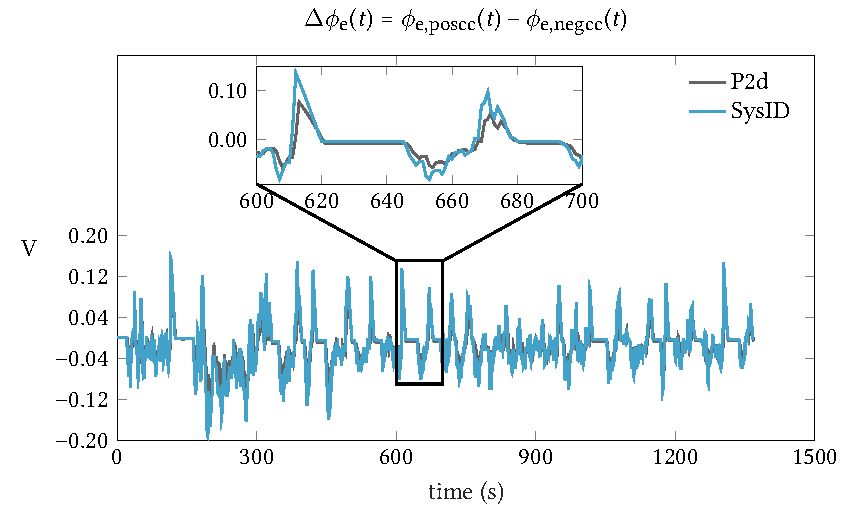
\includegraphics{phie_delta_udds.pdf}
    \caption[%
    Electrolyte  overpotential  computed  by the  \glsfmtshort{p2d}  and  system
    identification models for a \glsfmtshort{udds} load profile
    ]%
    {%
        Comparison    of    electrolyte    overpotential   computed    by    the
        \gls{p2d}     model    and     the    system     identification    model
        (using \cref{eq:electrolytepdwithcenew}) for a  \gls{udds} load profile.
        The overpotential  profile computed  by the system  identification model
        reasonably matches  that obtained  by the \gls{p2d} model  with a
        \glsfirst{mae} of \SI{15.88}{\milli\volt} and  a \glsfirst{rms} error of~\SI{24.11}{\milli\volt}.
    }%
    \label{fig:phiedeltacnstudds}
\end{figure}

Hence, it can be concluded  that the electrolyte overpotential computation using
the system identification  model provides an acceptable  performance for dynamic
load profiles.  The next step  is to incorporate this  electrolyte overpotential
calculation into the basic \gls{spm} and to quantify the voltage accuracy of the
resulting composite \gls{spm}.

\subsection{Terminal voltage computation of composite \glsfmtshort{spm}}

\addlines[0.5]
In \cref{subsec:simresultsbasicspm}, it  was shown that in  the basic \gls{spm},
the computation of the cell's \gls{soc}  is of sufficient accuracy. However, its
terminal  voltage  strongly deviates  from  the  true  value  as computed  by  a
\gls{p2d} model.  This mismatch between  \gls{soc} and terminal  voltage hinders
the  suitability of  the basic  \gls{spm}  as the  plant model  in online  state
estimation applications. The discrepancy in terminal  voltage is due to the lack
of electrolyte overpotential contribution in  its computation. Having obtained a
suitable methodology  to compute this  (see \cref{subsec:electrolyteopcalc}), it
is now possible to refine the computation of the cell's terminal voltage.

Referring   to \cref{eq:posoverpotential}  and \cref{eq:negoverpotential},   the
reaction overpotential in each of the two porous electrode regions is given by
\begin{align}
    η_\text{pos} &= ϕ_\spos - ϕ_\epos - U_\text{pos} \label{eq:posoverpotentialoverall} \\% \tag{\cref{eq:posoverpotential} revisited}\\
    η_\text{neg} &= ϕ_\sneg - ϕ_\eneg - U_\text{neg} \label{eq:negoverpotentialoverall} %\tag{\cref{eq:negoverpotential} revisited}
\end{align}
wherein  the  contribution  from   the  electrolyte  potential  terms~$ϕ_\epos$
and~$ϕ_\eneg$ are no longer to be neglected.

Subtracting \cref{eq:negoverpotentialoverall}
from \cref{eq:posoverpotentialoverall}
\begin{align}
 η_\text{pos} - η_\text{neg} &= \underbrace{ϕ_\spos - ϕ_\sneg}_{V_\text{cell}} - ϕ_\epos + ϕ_\eneg - U_\text{pos} + U_\text{neg}\\
\shortintertext{whose rearrangement yields}
V_\text{cell} &= η_\text{pos} - η_\text{neg} + \underbrace{ϕ_\epos -
ϕ_\eneg}_{\Delta \phi_\text{e}} + U_\text{pos} -
U_\text{neg}\label{eq:intermediatevoltagewithphie}
\end{align}

\addlines[0.5]
Substituting for ${\Delta \phi_\text{e}}$ from \cref{eq:electrolytepdwithcenew} in
into \cref{eq:intermediatevoltagewithphie},  and  expanding  each of  its  terms
(see derivation of \cref{eq:spmbasicoutputvoltagefinal}  for details), the final
expression for the cell's terminal voltage is obtained as
\begin{multline}
    V_\text{cell}(t) = \frac{2 R T}{F }\sinh^{-1} \left( \frac{- I(t)}{2 A l_\text{pos} a_\spos F k_\posr \sqrt{c_\text{e} c_\spossurf(t) \left(c_\sposmax - c_\spossurf(t)\right)}}\right) \\
    - \frac{2 R T}{F }\sinh^{-1} \left( \frac{I(t)}{2 A \, l_\text{neg} a_\sneg F k_\negr \sqrt{c_\text{e} c_\snegsurf(t) \left(c_\snegmax - c_\snegsurf(t)\right)}}\right) \\
    \hphantom{\text{hello worl}}+ (1-t_{+}^0) \frac{2RT}{F}\ln \frac{c_\text{e,\tiny pos/cc}(t)}{c_\text{e,\tiny neg/cc}(t)} -\frac{I}{2 A}\left(\frac{l_\text{neg}}{\kappa_\text{eff,neg}\left(c_\text{e}\left(0\right)\right)} + 2 \frac{l_\text{sep}}{\kappa_\text{eff,sep}\left(c_\text{e}\left(0\right)\right)} +
\frac{l_\text{pos}}{\kappa_\text{eff,pos}\left(c_\text{e}\left(0\right)\right)}\right)\\
    + \mathcal{U}_\text{pos}\left(c_\spossurf(t)\right) - \mathcal{U}_\text{neg}\left(c_\snegsurf(t)\right)\label{eq:spmcompositeoutputvoltagefinal}
\end{multline}

All  other   expressions  and  computations   of  the  basic   \gls{spm}  remain
unchanged (see \cref{sec:spmmodeldevelopment} for the  complete set of equations
constituting the model). The final step  is to show that the composite \gls{spm}
thus obtained has an improved performance especially in those scenarios that the
basic \gls{spm} performed poorly.

\subsection{Validation of composite \glsfmtshort{spm}: Terminal voltage accuracy}

The final  step in  this model  development effort is  the validation  phase. In
particular, the voltage accuracy of  the composite \gls{spm} is compared against
the  \gls{p2d} model  for standard  input conditions.  In order  to compare  and
contrast the  gains achieved  by the composite  \gls{spm}, the  terminal voltage
output of the basic \gls{spm} is also considered here.

\subsubsection*{Constant Current Inputs}

The  voltage  accuracy of  the  newly  developed  composite \gls{spm}  is  first
evaluated for  the standard test  case of 1C~discharge current starting  from a
cell \gls{soc} of~\SI{100}{\percent}.

\begin{figure}[!htb]
    \centering
    \includegraphics{composite_spm_vcell_1C.pdf}
    \caption[%
    Comparison  of  terminal  voltages  of  composite  \glsfmtshort{spm},  basic
    \glsfmtshort{spm} and the \glsfmtshort{p2d} model for a 1C~discharge
    ]%
    {%
        Voltage output  of various \glspl{spm}  for a 1C~discharge  beginning at
        \SI{100}{\percent} \gls{soc} (top  plot). Since it does  not account for
        electrolyte overpotentials,  the voltage  profile computed by  the basic
        \gls{spm} lies above that of the benchmark \gls{p2d} model. On the other
        hand, the composite \gls{spm} tends  to over correct for the electrolyte
        overpotential  so that  its terminal  voltage lies  below the  \gls{p2d}
        output. Since  the two \glspl{rom}  have outputs  on either side  of the
        \gls{p2d}  model,  it  is  convenient  to  use  the  absolute  error  to
        compare  them. In  the  bottom  plot, the  percentage  deviation of  the
        absolute error of the two  \glspl{rom} is shown. The composite \gls{spm}
        performs  significantly better  with a  peak absolute  error of  \approx
        \SI{4}{\percent} in  contrast to nearly \SI{11}{\percent}  for the basic
        \gls{spm}.
    }%
    \label{fig:voltageoutputcompareallSPMs1C}
\end{figure}

\Cref{fig:voltageoutputcompareallSPMs1C}  shows the  terminal voltage  output of
various \glspl{spm} for a 1C~discharge beginning at \SI{100}{\percent} \gls{soc}
(top  plot). Since  it  does  not account  for  electrolyte overpotentials,  the
voltage profile computed by the basic \gls{spm} lies above that of the benchmark
\gls{p2d}  model. On  the  other hand,  the composite  \gls{spm}  tends to  over
correct  for the  electrolyte overpotential  so that  its terminal  voltage lies
below  the \gls{p2d}  output. Since  the output  of the  two \glspl{rom}  lie on
either side of the \gls{p2d} model, it  is appropriate to use the absolute value
of their errors with respect to the  \gls{p2d} benchmark to compare them. In the
bottom  plot,  the  percentage  deviation  of the  absolute  error  of  the  two
\glspl{rom} is shown. The statistics of this deviation is quantified
in \cref{tbl:errorsummarycntcurrdischgallspms} which additionally includes the
performance metrics from the quadratic approximation \gls{spm}.

% -*- root: ../main.tex -*-
%!TEX root = ../main.tex
% this file is called up by main.tex
% content in this file will be fed into the main document
% vim:textwidth=180 fo=cqt

\begin{table}[!htbp]
    \caption[%
    Summary of error statistics for basic \glsfmtshort{spm} and composite \glsfmtshort{spm} for 1C discharge
    ]%
    {%
    Summary of statistics for the percentage absolute error
        in terminal voltage
    for the basic \glsfmtshort{spm} and the composite \glsfmtshort{spm} in constant current 1C discharge simulations.
}%
    \label{tbl:errorsummarycntcurrdischgallspms}
    \centering
    \begin{tabular}{@{} l S[table-format=2.2] S[table-format=1.2] @{}}
        \toprule
        \makecell{Error Statistic \\ for \si{\percent}$\abs{\hat{\varepsilon}_v}$} & {\makecell{Basic \\ \glsfmtshort{spm}}} & {\makecell{Composite \\ \glsfmtshort{spm}}} \\
        \midrule
        %
        Worst Case        & 10.67 & 4.05 \\
        Mean              & 2.92  & 1.54 \\
        \glsfmtshort{rms} & 3.27  & 1.65 \\
        %
        \bottomrule
    \end{tabular}
\end{table}


In  each of  the error  statistic considered,  the composite  \gls{spm} performs
significantly better than the basic \gls{spm} for the 1C~discharge case.

One   of   the   biggest   drawbacks   of   the   conventional   \gls{spm}   was
its    poor    voltage    accuracy    at    moderate    C-rates    above~0.5C
(see \cref{tbl:errorsummarycntcurrdischgspmp2d}). The high accuracy achieved for
the 1C~rate  seems to indicate that  the composite \gls{spm} is  indeed a viable
solution for all  high C-rates, especially given the backdrop  of its methodical
derivation steeped in system identification.

However,  there exists  a  fundamental  flaw in  all  models  that use  a~priori
assumptions  of  simplified spatial  profiles  for  ionic concentration  in  the
electrolyte.  In  the  case  of  both the  baseline  quadratic  and  the  system
identification models, a parabolic profile spanning the entire thickness of each
region within the cell was chosen a~priori. However, no attempt to modify the
profile upon encountering an ion starvation event at any spatial location.

This  critical flaw  is  exposed  by the  sustained  application  of any  higher
current  that  induces  an  ion  starvation at  one  of  the  electrodes  during
operation. \Cref{fig:2Cionstarvation}  depicts  the  ionic concentration  in  the
electrolyte  over  time at  both  current  collectors  for a  2C~discharge.  The
profiles  computed  by  both  the \gls{p2d}  and  system  identification  models
are  plotted.  For  the  system  identification  model,  the  current  collector
interface  at  the  positive  electrode  experiences  an  ion  starvation  event
at~\approx\SI{150}{\second}. The  quadratic spatial  profile used by  this model
does not account for such a  reduction in the effective electrode thickness. All
the  boundary conditions  and coefficients  were formulated  using the  original
electrode  thickness.  Therefore,  beyond \SI{150}{\second},  the  concentration
becomes negative which  is not physically meaningful. The author  of this thesis
has implemented a saturation mechanism in the code that detects an ion depletion
event and prevents the concentrations from becoming negative.

\begin{figure}[!htbp]
    \centering
    \includegraphics[width=\textwidth]{problematic_2C_conc.pdf}
    \caption[
    Time evolution of ionic concentration computed by the \glsfmtshort{p2d} and system
    identification models at both current collectors for a 2C~discharge
    ]
    {%
        Time evolution of ionic concentration in electrolyte computed by the \gls{p2d} and
        system identification models at ---
        \begin{enumerate*}[label=\emph{\alph*})]
            \item negative current collector interface (left plot), and
            \item positive current collector interface (right plot)
        \end{enumerate*}
        for a constant current discharge at \SI{120}{\ampere} \ie~2C. In the
        system identification mode, ion
        starvation occurs at the positive current collector interface at~\approx\SI{150}{\second}. The quadratic spatial profile used by the system
        identification model spans the entire electrode region and does not
        account for ion depletion scenarios. In this thesis, the author has
        implemented a saturation mechanism in the computer code to prevent the
        ionic concentration from becoming negative. Despite this
        mitigating action, the computation of electrolyte overpotential
        using \cref{eq:electrolytepdwithcenew} is problematic in such scenarios.
    }%
    \label{fig:2Cionstarvation}
\end{figure}

\addlines[0.5]
Implementing  this  hard   lower  bound  of  zero  for   the  ion  concentration
does    not   mitigate    the   problems    associated   with    computing   the
electrolyte   overpotential.   Specifically,  computational   difficulties   are
encountered    when   computing    the    concentration   dependent    diffusion
overpotential \cref{eq:electrolytepdwithcenew}. In the case  of ion depletion at
the positive  current collector,  the argument of  the logarithmic  term becomes
zero which leads to a non-feasible computation~($-\infty$). Ion depletion at the
negative current collector  is equally detrimental to  the computation. However,
this scenario has  a lower probability owing to the  low C-rates during charging
operation (see \cref{subsec:basicspmsimsetup}).  Furthermore, in the  absence of
the lower  bound of zero  for the  concentrations, complex numbers  are obtained
from  the logarithmic  term, which  lead to  physically erroneous  overpotential
calculations. An  alternative is  to simply omit  the diffusion  impedance term.
However, since  this term is  responsible for  the large-signal dynamics  of the
overpotential (see \cref{fig:contributiontophiefromtwoterms}), omitting this and
reverting to  a simple ohmic  resistance contribution shall lead  to significant
errors  in  the electrolyte  overpotential,  and  consequently in  the  terminal
voltage.  Finally, setting  the diffusion  impedance to  zero at  the transition
boundary of ion starvation is also not a feasible solution. This is because, the
sudden inflection in  the trajectory of the terminal voltage  shall induce large
errors in any state estimation algorithms that depend on the composite \gls{spm}
as the plant model.

\addlines[0.5]
The  difficulties  encountered  in electrolyte  overpotential  computations  for
ion  depletion scenarios  have  not  yet been  discussed  in  the literature  by
the  research  community that  use  such  quadratic approximation  models.  This
thesis author  therefore assumes that  such a  scenario had not  been previously
encountered  for  the  parameter  set  and C-rate  combinations  used  by  those
researchers. Despite the  fact that this phenomenon might be  an artefact of the
idiosyncrasies of the  parameter set used here, it  is nevertheless questionable
to not  have mathematically adapted  the parabolic  profile to such  events. The
aspect  of rendering  the model  robust to  such vagaries  is currently  an open
problem in the field and can be the subject of future research. It can therefore
be concluded that  this composite \gls{spm} is \emph{unsuitable}  in its present
form for  sustained constant current  discharge at higher C-rates.  Despite this
setback due  to deficiencies in  the mathematical formulation of  the underlying
spatial profile, the superior performance  of the system identification model in
the computation  of ionic  concentrations and overpotentials  for \emph{dynamic}
conditions warrant such a study for the composite \gls{spm}.



\subsubsection*{Dynamic Load Conditions}

\addlines[0.5]
In  order to  evaluate the  performance of  the composite  \gls{spm} to  dynamic
inputs, the  input profile  corresponding to  the \gls{udds}  drivecycle profile
in \cref{fig:uddssimp2dspmresults}  with  a  peak current  of  \SI{180}{\ampere}
\ie~3C was used.

\Cref{fig:voltageoutputcompareallSPMsudds}  shows  the  voltage  output  of  the
composite  \gls{spm}  for a  \gls{udds}  input  profile  with a  peak  magnitude
of   \SI{180}{\ampere}  \ie~3C  (see \cref{fig:uddssimp2dspmresults}).   The
voltage   profiles  computed   by  the   basic  \gls{spm}   and  the   benchmark
\gls{p2d}  model   is  also  overlaid   (top  plot).  The   percentage  absolute
error  of  the  two  \glspl{rom}  relative  to  the  \gls{p2d}  model  is  shown
in  the  bottom  plot.  It  is  seen  that  the  terminal  voltage  of
the  composite  \gls{spm}   is  more  accurate   than  the  basic
\gls{spm}  (see \cref{tbl:errorsummaryuddsdischgallspms}, which additionally
includes the performance metrics from the quadratic \gls{spm}).   For  instance,  the
voltage  profile  computed by  composite  \gls{spm}  matches the  complex  shape
characteristics  of the  \gls{p2d} model  while remaining  very close  to it  in
magnitude.

\begin{figure}[!htb]
    \centering
    \includegraphics[width=0.6375\textwidth]{composite_spm_vcell_udds-crop.pdf}
    \caption[%
    Terminal voltage output of --- \emph{a}) the \glsfmtshort{p2d} model, \emph{b}) the
    basic \glsfmtshort{spm}, and \emph{c}) the composite \glsfmtshort{spm} for a
    \glsfmtshort{udds} input profile
    ]%
    {%
        Voltage output of the composite \gls{spm} for a \gls{udds} input profile
        with a peak magnitude of \SI{180}{\ampere} \ie~3C
        (see \cref{fig:uddssimp2dspmresults}). The voltage
        profiles computed by the basic \gls{spm} and the benchmark \gls{p2d}
        model is also overlaid (top plot). The percentage absolute error of the
        two \glspl{rom} relative to the \gls{p2d} model is shown in the bottom
        plot. The terminal voltage of the composite \gls{spm} is significantly
        more accurate than the basic \gls{spm}
        (see \cref{tbl:errorsummaryuddsdischgallspms}).
    }%
    \label{fig:voltageoutputcompareallSPMsudds}
\end{figure}

% -*- root: ../main.tex -*-
%!TEX root = ../main.tex
% this file is called up by main.tex
% content in this file will be fed into the main document
% vim:textwidth=180 fo=cqt

\begin{table}[!htbp]
    \caption[%
    Error statistics for basic  and composite \glsfmtshortpl{spm} for a \glsfmtshort{udds} load profile
    ]%
    {%
    Summary of statistics for the percentage absolute error
        in terminal voltage
        for the basic \glsfmtshort{spm} and the composite \glsfmtshort{spm} with \gls{udds} input profile.
}%
    \label{tbl:errorsummaryuddsdischgallspms}
    \centering
    \begin{tabular}{@{} l S[table-format=2.2] S[table-format=1.2] @{}}
        \toprule
        \makecell{Error Statistic \\ for \si{\percent}$\abs{\hat{\varepsilon}_v}$} & {\makecell{Basic \\ \glsfmtshort{spm}}} & {\makecell{Composite \\ \glsfmtshort{spm}}} \\
        \midrule
        %
        Worst Case        & 2.59 & 0.72 \\
        Mean              & 0.51 & 0.11 \\
        \glsfmtshort{rms} & 0.68 & 0.16 \\
        %
        \bottomrule
    \end{tabular}
\end{table}


% Conclude the chapter  by saying that everything is now  in time domain. Suitable
% for direct  implementation. Concludes the  implementation aspect of  the thesis.
% Can now be used as the plant model in EKF and other applications.



             % New Electrolye Model
\setcounter{chapter}{6}
 % -*- root: ../../main.tex -*-
% !TEX root = ../../main.tex
% vim:textwidth=80 fo=cqt

\graphicspath{{chapters/litt_review/figures/}}
% ----------------------- contents from here ------------------------

\clearpage
\chapter{Conclusions}\label{ch:conclusions}
\startcontents[chapters]
\printcontents[chapters]{}{1}{\setcounter{tocdepth}{2}}

\bigskip

\capolettera{I}{n} this  thesis, the  deployment of  physics-based computational
modelling  of lithium  ion  cells  for electric  vehicle  applications has  been
rigorously examined with a three-pronged strategy \viz{} through their analysis,
design and implementation. Salient conclusions  drawn from each of these aspects
are presented  in this  chapter. The \gls{p2d}  implementation of  the \gls{dfn}
model was used  as the backbone of  all modelling efforts in  this thesis. Based
upon the  invaluable experience gained during  the course of this  research, and
specifically from the  findings presented herein, key areas  of \glspl{pbm} that
can benefit from further study in the future are also identified.

% These are discussed in-line at the appropriate junctures embedded into the narrative.

\section{\glsfmtlongpl{pbm} as a Design Tool}

\subsection{Conclusions from the model-based design study}\label{sec:modelbasedconclusion}

\Cref{ch:modelbaseddesign} presented  a computational framework to  optimise the
number  of electrochemical  layers to  be  used within  a  pouch cell  so as  to
maximise its usable energy while  meeting specific power demands. In particular,
this  helped to  construct  a model-based  deterministic  approach to  optimally
design cells  that can  be subjected  to fast-charging  without the  concerns of
plating. In  the context of  electric vehicle applications, using  this approach
has the  potential to alleviate  the two  immediate concerns of  consumers viz{}
range anxiety and long charging times.

To facilitate immediate adoption by relevant stakeholders, the concepts presents
in the aforementioned optimisation framework  has been realised in computer code
and presented  in the form  of an  open-source design toolbox,  \gls{bold}. This
toolbox  was  applied to  the  optimal  layer design  of  an  example cell  from
literature to  obtain two sets  of power-dependent optimal  layer configurations
for two drivetrains  --- a \gls{bev} and a \gls{phev}.  By suitably adapting the
numerical values  of parameters to  a real-world cell, model-based  cell designs
can be  obtained, which can potentially  help to eliminate the  current trend of
over-engineering of cells using conservative empirical designs.

From a  perspective of technical  advancements to the underlying  \gls{pbm}, the
standard form  of the \gls{p2d} model  has been suitably modified  to facilitate
a  direct  application of  input  power  densities.  This was  achieved  through
reformulation of the boundary conditions on the solid-phase potential \gls{pde}.
Although  this innate  power input  capability has  been claimed  as purportedly
developed,  its independent  derivation  and  accessible documentation  provided
herein shall help  other researchers to apply this in  a straight-forward manner
for vehicle drivecycles, acceleration tests and power-based charging protocols.

This investigation also  revealed that the fast charging  process determines the
optimal layer  configuration instead of  either acceleration runs  or drivecycle
requirements. This may  help to counter the current trend  in publications which
often rely  primarily upon a  drivecycle-based dynamic input current  profile to
evaluate various  aspects of cell  modelling such as predicting  degradation and
for advanced control and estimation  algorithms. While validation against such a
dynamic input profile  is certainly vital, for future  advancements dealing with
aspects  of  cell  design  or plating-related  degradation,  validation  against
fast-charging power profiles is absolutely essential.

The  study also  provided important  guidelines about  the role  of the  thermal
environment on cell performance. It became  clear that at very low temperatures,
a high  number of layers was  required for satisfying a  specific charging power
level relative  to that  needed at  moderate thermal  environments such  as room
temperatures. A practical  takeaway from this conclusion is that  it suffices to
use a low number of layers in  vehicles to be sold in territories with perennial
moderate  temperature  conditions, which  imply  a  higher \gls{aer}  for  these
vehicles.

Finally, this design study revealed that the speed at which lithium intercalates
into the negative  electrode during charging limits the  charge-addition rate to
the cell and hence to the pack. Lowering the charging times of electric vehicles
necessitates the  use of  higher charging powers.  However, this  necessitates a
high  number of  layers to  absorb the  overpotentials and  to provide  adequate
number of  thermal conduction pathways  (owing to  the higher number  of current
collectors) to dissipate the additional heat generated. Consequently, this has a
detrimental effect on the capacity and hence, the \gls{aer} of the vehicle.

\subsection{Future work informed by  the optimal layer design framework}

As     a     direct     inference     of     the     final     conclusion     in
\cref{sec:modelbasedconclusion}, assuming that  the electric grid infrastructure
is  adequately equipped  to cope  with  the surge  in future  power demands  for
charging  of  electric vehicles,  the  solid  state  diffusion at  the  negative
electrode becomes the bottleneck. It  is therefore important for future research
to  focus  on the  development  of  new  materials  for the  negative  electrode
possessing much higher  solid phase diffusion coefficients,  particularly at low
temperatures.

From a perspective of improving the framework itself, at the outset, it is clear
that the plating threshold assessment can be made more accurate by incorporating
the solid phase diffusion coefficient as  function of \gls{soc}. In the interest
of simplicity and  to lay the foundation for such  model-based cell designs, the
scope of this  work was intentionally narrowed down to  solely focus on changing
the layer  configurations within  cells. In doing  so, certain  assumptions were
made  that  might have  to  be  revisited  and  potentially relaxed  before  its
application to real-world cell designs.

For instance, adherence to the specific type of cooling phenomena used \ie{} tab
cooling, is one of  the stronger assumptions used in this  work. The benefits of
this cooling  type has  been enumerated,  and it is  desirable that  future pack
designs adopt it. However, the vast majority of battery packs use surface-cooled
designs. This means  that temperature for all layers within  the pouch shall not
be the same,  which further implies that  it longer suffices to  simulate just a
single layer. Therefore,  the framework needs to be suitably  modified to handle
multiple layer choices concurrently.

Furthermore,  using surface  cooling shall  invalidate the  assumption of  small
thermal gradients along the planar axis of  the cell. This means that the lumped
thermal model  shall no longer  be accurate  to model the  temperature evolution
of  the cell.  Furthermore,  the differential  temperature  evolution along  the
cross-sectional direction  shall influence the transport  and kinetic properties
of the  cell. This electrochemical-thermal  coupling along the  planar direction
shall necessitate adding another spatial  dimension to the underlying \gls{pbm},
thereby rendering the  presently used \gls{p2d} model ineffective.  With the aim
of minimising  the optimising  run-times, future  research may  focus on  how to
adapt the proposed computational infrastructure from this thesis to handle this.

For  real-world cell  designs, it  is prudent  to examine  the examine  the role
of  variable  porosities  to  achieve  the balancing  of  active  materials  per
layer.  Since  the computational  framework  developed  in  this thesis  uses  a
modular  approach, in  the future,  the  constant volume-fractions  used in  the
methodology  could simply  be replaced  by values  informed by  optimal porosity
computations. For this purpose, researchers could investigate the feasibility of
adapting  a suitable  scheme from  the available  pool of  literature that  have
focussed  on  using  model-based  porosity  optimisation~\cite{Xue2013,Xue2014a,
Christensen2006}. Finally, experimental prototyping is  an important step in any
cell  design and  it  is  no exception  here  either. Therefore,  experimentally
applying the desired power levels to confirm the optimal layer choices predicted
by the  framework is an important  step to be undertaken  before its large-scale
deployment.





\section{Analysis of Salient Physics-based \glsfmtlongpl{rom}}

Chapters~\ref{ch:improveddra} and~\ref{ch:spmanalysis} of  this thesis primarily
focussed on performing an in-depth analysis of two distinct \glspl{pbm} from two
distinct perspectives.  In \cref{ch:improveddra}, the hybrid  \gls{rom} obtained
by  using the  \gls{dra}  is analysed  to  investigate its  \emph{computational}
bottlenecks.  In \cref{ch:spmanalysis},  an  in-depth analysis  of the  simplest
time-domain physics-based \gls{rom} --- the  \gls{spm} --- is presented from the
perspective of \emph{modelling accuracy} \ie{} its ability to faithfully compute
the  system-level quantities  of the  cell such  as its  \gls{soc} and  terminal
voltage. The conclusions drawn from these analyses are presented here.

\subsection{Conclusions from analysis of the \glsfmtshort{dra}-based state-space \glsfmtshort{rom}}

In  \cref{ch:improveddra},  the \gls{svd}  of  a  large Block-Hankel  matrix  is
identified as a key computational bottleneck in applying the classical \gls{dra}
procedure for the hybrid \gls{rom} discussed  therein. It is concluded that this
bottleneck arises due to the slow  dynamics of solid phase diffusion which leads
to the aforementioned large sized Block-Hankel matrices.

To mitigate this  bottleneck, an improved \gls{dra} scheme  was presented, whose
centrepiece is an iterative \gls{svd}  algorithm. This algorithm was obtained as
a  combination of  the Golyandina-Usevich  and Lanczos  algorithms discussed  in
\cref{ch:improveddra}.  The results  of applying  the improved  \gls{dra} scheme
demonstrate  a significant  performance improvement  achieved by  using the  new
method  without trading-off  model  fidelity.  At a  single  operating point  of
\gls{soc}  and temperature,  for  a  Hankel block  size  of~8000, the  \gls{rom}
workflow incorporating the improved  \gls{dra} is approximately 100~times faster
than  that employing  classical \gls{dra}.  On a  standard computer  workstation
whose  specifications  are  given in  \cref{ch:improveddra},  for  100~operating
points  (combinations of  10~\gls{soc}  and temperature  values), obtaining  the
\gls{rom}  required  only 6~hours  using  the  improved \gls{dra},  whereas  the
classical  \gls{dra} consumed  666~hours  (27~days). Furthermore,  for the  same
block-size, the  improved \gls{dra} is demonstrated  to be superior in  terms of
memory efficiency, drastically reducing the memory requirements from 112~GB down
to  2~GB.  Finally,  the  improved  \gls{dra}  demonstrates  superior  modelling
accuracy  when implemented  even in  moderately equipped  computing environments
such as standard consumer-grade laptops.

\subsection{Future outlook for the \glsfmtshort{dra}-based hybrid state-space \glsfmtshort{rom}}

The improved  \gls{dra} method  proposed in  \cref{ch:improveddra} opens  up the
possibility of  applying the  hybrid \gls{rom}  modelling procedure  to physical
quantities in other locations within the  cell's geometry \eg{} in the middle of
the electrode region,  without being hindered by  computational limitations that
would  have otherwise  rendered  it intractable.  Furthermore, high  sample-rate
\glspl{rom} capable  of handling  highly dynamic load  profiles can  be deployed
in  future  \gls{bms}  applications.  The  proposed  scheme  also  empowers  the
\gls{rom}  framework to  tackle  other cell  chemistries  with slower  diffusion
coefficients or  even those with completely  different rate-limiting mechanisms.
The improved \gls{dra}  method therefore opens up a wide  range of possibilities
and  prima~facie looks  capable of  bringing the  goal of  physics-based battery
model implementation in a high performance real-time \gls{bms}, a step closer to
realisation.

Despite   the  aforementioned   euphoric   possibilities   facilitated  by   the
streamlining  of  the reduced  order  modelling  workflow through  the  improved
\gls{dra},  there  exists a  fundamental  deficiency  in this  hybrid  modelling
approach  that impede  its  effective deployment  as the  plant  model in  state
estimation tasks. This aspect was already discussed in \cref{ch:littreview}, and
is  reiterated here.  The  entries in  the  matrices of  the  final state  space
model  depend on  the linearisation  point  of \gls{soc}  and temperature.  This
linearisation requirement adversely affects the usability of the model for state
estimation tasks, wherein the \gls{soc} is in fact an unknown quantity and is to
be  estimated.  This  cyclic  dependency between  the  linearisation  point  and
the  state-estimation quantity  makes  the  use of  this  model questionable  in
a  demanding  application such  as  in  embedded \glspl{bms}  on-board  electric
vehicles.


\section{Closing Remarks}

% closing remarks
% Parametrisation is a problem as well.
% solid-state diffusion is a problem informed by two chapters. Need advanced
% materials
% By  reducing the  time  for final  prototyping
% through replacement  of expensive  experimental iterations,  cost-effective cell
% manufacturing paradigms can  be ushered, which can be passed  on to customers of
% electric vehicles. This in-turn can  help to accelerate the mass-market adoption
% of electrified transport.

% This approach reduces the cost as well as time expenditure required by an
% automotive OEM. This adds a new xEV to their product range, speeding up  for a
% cleaner, safer and  decarbonised transport.


% % through   . that can  help to unleash  the latent  potential of lithium ion batteries has been studied

% achieve the latent  potential and wide applicability  of the
% physics-based reduced order Li-ion battery model.


   % Conclusions

\backmatter
\singlespacing
\begin{footnotesize} % Bibliography/References
    \renewcommand{\bibname}{References} % changes the header; default: Bibliography
    % add bib to toc
    \cleardoublepage
    \phantomsection
    \addcontentsline{toc}{chapter}{\bibname}
    \printbibliography
\end{footnotesize}

% Required to maintain continuous arabic numbering
\makeatletter
\@mainmattertrue
\makeatother
\cleardoublepage


% \setstretch{1.348361657291667} % golden-ratio stretch (1.2 x 1.348 = 1.618)
\begin{appendices} % Using the appendices environment (from appendix package) for more functionality
    \crefalias{chapter}{appchap}
    % -*- root: ../main.tex -*-
%!TEX root = ../main.tex
% vim: nospell

% ******************************* Thesis Appendix A ****************************
\chapter{Full Listing of Program Codes}

% dummy cts time \label{sc:ctstimespm}
\glsdisablehyper
\matlabcodelisting[\textsc{MATLAB} code for simulation of continuous time \glsfmtshort{spm}]{chapters/Appendices/matlab_codes/cts_time_spm_simulation.m}{sc:ctstimespm}

% dummy disc time\label{sc:disctimespm}
\clearpage
\matlabcodelisting[\textsc{MATLAB} code for simulation of discrete time \glsfmtshort{spm}]{chapters/Appendices/matlab_codes/disc_time_spm_simulation.m}{sc:disctimespm}
\glsenablehyper


% graphviz doc in appendix, toolbox, directory listing etc.

    % -*- root: ../../main.tex -*-
%!TEX root = ../../main.tex
% vim: nospell

% ******************************* Thesis Appendix A ****************************
\chapter{Permissions Summary}\label{ch:permissions}
\startcontents[chapters]
\printcontents[chapters]{}{1}{\setcounter{tocdepth}{1}}

\fakesection{Permissions Table}
% -*- root: ../../main.tex -*-
%!TEX root = ../../main.tex

\begin{sidewaystable}
    \caption{Summary of permissions for reuse of third-party copyrighted material}
    \label{tbl:permissionstable}
    \centering
	\begin{scriptsize}
	    \begingroup
	    \renewcommand{\arraystretch}{2}
	    \begin{tabular}{@{} l l l p{8.65cm} l c c p{2.5cm} @{}}
            \toprule
            \multicolumn{1}{c}{\makecell{Page \\ no.}} & \makecell{Type of \\ work} & \makecell{Usage in \\ thesis} & \makecell{Source \\ \vphantom{of work}} & \makecell{Copyright holder \& \\ Contact (organisations only)} & \makecell{Permission \\ requested on} & \makecell{Have \\ permission?} & \makecell{Permission \\ remarks} \\
            \midrule

            \cpageref{fig:energyvspowercell}       & figure & \Cref{fig:energyvspowercell}       & \fullcite{VonSrbik2015} & \Citeauthor*{VonSrbik2015} & N/A                  & Yes & CC-BY-NC-ND                       \\
            \cpageref{fig:fig_CC_discharge_curves} & figure & \Cref{fig:fig_CC_discharge_curves} & Unpublished work        & Ian D.\ Campbell           & \DTMdate{2018-09-28} & Yes & Written agreement                 \\
            \cpageref{fig:1d_fv_mesh}              & figure & \Cref{fig:1d_fv_mesh}              & \fullcite{Torchio2016}  & \Citeauthor{Torchio2016}   & \DTMdate{2018-09-28} & Yes & \makecell[l]{`Rightslink' service \\ agreement attached} \\

            \bottomrule
        \end{tabular}
        \endgroup
    \end{scriptsize}
\end{sidewaystable}



\cleardoublepage

\fakesection{Copyright Permissions for Torchio~\etal}
\includepdf[pages=-,scale=0.85,pagecommand={}]{chapters/Appendices/redacted_JES_Torchio_permission_pdf.pdf}
\fakesection{Copyright Permissions for Northrop~\etal}
\includepdf[pages=-,scale=0.85,pagecommand={}]{chapters/Appendices/redacted_Northrop_permission_pdf.pdf}
\fakesection{Copyright Permissions for Moura~\etal}
\includepdf[pages=-,scale=0.925,pagecommand={}]{chapters/Appendices/redacted_Moura_etal_permissions.pdf}
\fakesection{Copyright Permissions for Gopalakrishnan~\etal}
\includepdf[pages=-,scale=0.925,pagecommand={}]{chapters/Appendices/asme_copyright.pdf}
\fakesection{Copyright Permissions for Deng~\etal}
\includepdf[pages=-,scale=0.85,pagecommand={}]{chapters/Appendices/redacted_Deng_copyright.pdf}
\fakesection{Copyright Agreement --- Krishnakumar Gopalakrishnan and Ian D.\ Campbell}
\includepdf[pages=-,scale=0.85,pagecommand={}]{chapters/Appendices/campbell_krishna_agreement.pdf}





\end{appendices}

\batchmode
\end{document}
